\documentclass[12pt]{article}
\usepackage[T1]{fontenc}
%\usepackage[utf8]{inputenc}  Encodage UTF-8
\usepackage{amsmath}
\usepackage{amssymb}
%\usepackage[a4paper, margin=1in]{geometry}
\usepackage{setspace}
\usepackage{listings}
\usepackage{amsthm}
\usepackage{pgfplots}
\pgfplotsset{compat=1.18} % S'assurer d'utiliser une version récente de PGFPlots
\usepackage{longtable}
\usepackage{amsfonts}
\usepackage{adjustbox}
\usepackage{Pstricks}
\usepackage{lipsum}  % Pour du texte d'exemple
\usepackage{lettrine}
%\usepackage{Pscript}
\usepackage{tkz-tab}
\usepackage{changepage}
\usepackage{pdflscape}
\usepackage{hyperref}
\usepackage{mathrsfs}
\usepackage{pst-plot}
\usepackage{graphicx}
\usepackage{asymptote}
\usepackage[a4paper,
    top=2cm,    % Marge supérieure
    bottom=2.5cm, % Marge inférieure
   left=3cm,   % Marge gauche
    right=2cm   % Marge droite
]{geometry}
\usepackage{tikz}
%\usepackage[margin=0cm]{geometry}  % Supprimer les marges
\usepackage{draftwatermark}
\SetWatermarkText{La RevueCapes} % Texte du filigrane
\SetWatermarkLightness{0.8} % Opacité (1 = clair, 0 = sombre)
\SetWatermarkScale{2} % Taille du filigrane

    
\begin{document}
\begin{spacing}{1.5}


%\begin{figure}[hbtp]
%\caption{Garde}
%\centering
%\includegraphics[scale=1]{PagesGardeCapes.png}
%\end{figure}

\newgeometry{left=0cm, right=0cm, top=0cm, bottom=0cm}% Suppression des marges
\begin{figure}[hbtp]
%\centering
\includegraphics[scale=1]{PG0.png}
\end{figure}

\restoregeometry %Restaurercles mages normales



%\begin{adjustwidth}{-3cm}{-2cm}%Reduction de marge de 2cm à gauche et à droite
%\includegraphics[width=\paperwidth, height=\paperheight, keepaspectratio]{PagesGardeCapes.png}
%\end{adjustwidth}
\newpage


\begin{center}

\textbf{A propos}
\end{center}

Ce document a été soigneusement élaboré pour accompagner les candidats dans leur préparation aux concours directs du  \textbf{CAP-CEG},  \textbf{ CAPES (\emph{ option Mathématiques}) et au recrutement sur mesure nouvelle} au Burkina Faso. Il s'agit d'une ressource pédagogique complète et pratique, conçue pour répondre aux besoins spécifiques des aspirants candidats à ces épreuves exigeantes. Dans la section dédiée aux mathématiques, le document propose un rappel complet des notions fondamentales, permettant de consolider les bases théoriques indispensables. Il inclut également 15 sujets types soigneusement élaborés, accompagnés de corrections détaillées et explicatives, ainsi qu'une collection des anciens sujets corrigés de 2016 à 2022, offrant une précieuse opportunité d'analyser les tendances des épreuves passées. Par ailleurs, la section consacrée à la culture générale met à disposition un cours approfondi sur la dissertation, conçu pour aider les candidats à maîtriser les techniques rédactionnelles et les exigences des épreuves écrites. Elle est enrichie de propositions de sujets types et des corrections des anciens sujets pour une mise en pratique efficace. Chaque exercice est traité de manière intégrale, avec des explications claires et progressives pour garantir une compréhension approfondie des notions et méthodes. Ce document se positionne ainsi comme un outil incontournable, offrant aux candidats un cadre structuré et méthodique pour aborder les concours avec confiance et maximiser leurs chances de succès.


\newpage
%Affiche table des matières

\section*{\textbf{A. RAPPELS DE MATHS}}

\subsection*{1.  Nombres complexes}
\subsection*{2. Équation différentielle}
\subsection*{3. Calcul intégral}
\subsection*{4. Probabilités}
\subsection*{1. Ensembles et structures algébriques}
\subsection*{2. Arithmétique élémentaire}
\subsection*{3. Structures algébriques}
\subsection*{4. Matrices et déterminants}
\subsection*{5. Systèmes d'équations linéaires}
\subsection*{6. Espaces vectoriels}
\subsection*{8. Valeurs propres et vecteurs propres}
\subsection*{10. L'intégrale Impropre}
\subsection*{11.Suites numériques}
\subsection*{12. Séries numériques}
\subsection*{13. Séries entières}
\subsection*{14. Fonctions à deux variables}
\subsection*{15. Développement limité}
\section*{\textbf{B. PROPOSITION DE SUJETS TYPES}}
\section*{\textbf{C. ANCIENS SUJETS CAPES}}
\section*{\textbf{D. CORRECTIONS DE SUJETS TYPES}}
\section*{\textbf{E. CORRECTIONS D'ANCIENS SUJETS}}
\section*{A. Principes}
\section*{B. Les différentes parties d'une dissertation}
\section*{C. Sujets types de dissertation}
\section*{\textbf{D. ANCIENS SUJETS DE CULTURE GÉNÉRALE}}
\section*{\textbf{E. PROPOSITIONS DE CORRECTIONS DES ANCIENS SUJETS DE CULTURE GÉNÉRALE}}









\newpage



\section*{\textbf{A. RAPPELS DE MATHS}}

\medskip
\subsection*{1.  Nombres complexes}

 L'ensemble des nombres complexes est : $\mathbb{C}=\{z=a+ib/(a;b)\in \mathbb{R}^2$ et $i^2=-1\}$
 
 \textbf{\underline{Définition et propriété}}
 
 \quad
 
\begin{table}[h!]
\centering
\resizebox{\textwidth}{!}{%Redimentionner à la largeur de la page
 \begin{tabular}{|c|}
 \hline 
La forme algébrique du nombre complexe $z$ est : $a+ib$ \\ 
 \hline 
  Le  nombre complexe $z$ est imaginaire pur si sa partie réelle $Re(z)=0$\\ 
 \hline 
 Le  nombre complexe $z$ est réel si sa partie imaginaire $Im(z)=0$ \\ 
 \hline 
 Égalité de deux nombres complexes : $z=z'\Leftrightarrow Re(z)=Re(z')$ et $Im(z)=Im(z')$ \\ 
 \hline 
 L'argument du nombre complexe non nul $z$ est toute mesure $\theta$ vérifiant $z=re^{i\theta}$  avec $r=\vert z\vert$ \\ 
 \hline 
 Soit $(z,z')\in (\mathbb{C}^*)^2$,
 
 
 $\begin{array}{c}
 -arg(zz')=arg(z)+arg(z')[2\pi]\\
 -arg(az)=arg(z)[2\pi] \text{ si } a \in \mathbb{R}_{+}^{*}\\
 -arg( az)=\pi+arg(z)[2\pi] \text{ si } a\in \mathbb{R}_{-}^{*}\\
 -arg(z^n)=n arg(z) [2\pi]\\
 -arg(\frac{	1}{z})=-arg(z)[2\pi]\\
 -arg(\frac{z}{z'})=arg(z)-arg(z')[2\pi]\\
 -arg(\overline{z})=-arg(z)[2\pi]
 \end{array}$\\
 \hline
 La forme trigonométrique du nombre complexe non nul $z$ est $\vert z\vert(\cos\theta+i\sin\theta)$\\
 \hline
 La forme exponentielle du nombre complexe non nul $z$ est : $z=\vert z\vert e^{i\theta}$ ou $\theta$ est un argument de $z$\\
 \hline
 Formule de Moivre : $e^{in\theta}=(\cos\theta+i\sin\theta)^n=\cos(n\theta)+i\sin(n\theta)$\\
 \hline
\textbf{ Formules d'Euler :}

 $\cos\theta=\frac{1}{2}(e^{i\theta}+e^{-i\theta})$ et $\sin\theta=\frac{1}{2i}(e^{i\theta}-e^{-i\theta})$ \\
 \hline
 \textbf{\underline{Transformations du plan :}}\\
\textbf{ Translation} du vecteur $\overrightarrow{u}$ d'affixe $z_{\overrightarrow{u}} : z'=z+z_{\overrightarrow{u}}$\\
\textbf{ Homothétie} de centre $\Omega(\omega)$ et de rapport $k$ : $z'-\omega=k(z-\omega)$\\
 \textbf{Rotation} de centre $\Omega(\omega)$ et d'angle $\theta$ : $z'-\omega=e^{i\theta}(z-\omega)$\\
 \hline
 \end{tabular}
 }
 \end{table}






\subsection*{2. Équation différentielle}

\quad


\checkmark \quad \textbf{\underline{Définitions}}

\quad  \begin{tabular}{|p{15cm}|}
\hline 
 \textbf{ Définition 1 :} On appelle équation différentielle linéaire du premier ordre $(E)$ sur un intervalle $I$,une 
équation qui peut se mettre sous la forme:
 $(E) : y'+a(x)y=b(x)$ où l'inconnue $y$ est une 
 fonction de $x$ dérivable que l'on cherche à déterminer et où $a$ et $b$ sont deux fonctions continue sur un intervalle $I$\\ 
\hline 
\end{tabular}

\quad

\quad  \begin{tabular}{|p{15cm}|}
\hline
\textbf{ Définition 2 :} On appelle équation différentielle linéaire du second ordre à
 coefficients constants $(E)$ sur un intervalle $I$, une équation qui peut se mettre sous
 la forme :
 
 $(E) : ay'' +by' +cy = d(x)$
 
 où l'inconnue $y$ est une fonction de $x$ dérivable deux fois que l'on cherche à déterminer et où $a, b, c$ sont des réels avec $a\neq 0$ et $d$ une fonction continue sur un
 intervalle $I$.\\ 
\hline 
\end{tabular}

\quad

\quad

\checkmark \quad \textbf{\underline{Résolution de l'équation différentielle}}
 

\begin{itemize}
\item \quad \textbf{Équation incomplète}\\
Les solutions de l'équation différentielle $y'=b(x)$ incomplète en $y$ sur $I$ sont toutes les fonctions $y : x \longmapsto B(x)$ o\'u $B$ est une primitive de la
 fonction $b$ sur $I$.
\item \quad \textbf{Équation homogène du premier ordre}\\
Soit $a(x)$ une fonction continue sur un intervalle $I$.
 Les solutions de l'équation différentielle homogène : $y'+a(x)y=0$, sont toutes
 les fonctions $y: x \longmapsto ke^{-A(x)}$, avec $A$ une primitive de $a$ sur $I$ et $k\in \mathbb{R}$.
 
 \item \quad \textbf{Équation linéaire du premier ordre}\\
  Soit $a$ et $b$ deux fonctions continues sur un intervalle $I$. Soit $A$ une primitive de la
 fonction $a$.\\
 Les solutions de l'équation différentielle $(E) : y' + a(x)y = b(x)$ sont les fonctions $y$ tels que : $y = y_p + ke^{-A}$, où $y_p$ est une solution particulière de l'équation $(E)$ et $k$ un réel déterminé par les conditions initiales.\\
\textbf{Remarque :} Pour trouver toutes les solutions de l'équation $(E)$, il suffit de trouver une solution particulière et de lui ajouter la solution générale de l'équation homogène. Pour trouver cette solution particulière, on utilisera la méthode de la $\ll$ variation $\gg$ de la constante.\\
\item \quad \textbf{ Équation linéaire à coefficients constants}\\
 Soit $a$ et $b$ deux réels. Les solutions de l'équation différentielle: $y'+ay=b$ sont les fonctions $y$ de la forme:
 $y(x)=ke^{-ax}+\frac{a}{b}$.
\item \quad \textbf{Équation homogène du second ordre}\\ 
 Soit $(E)$ une équation différentielle linéaire du second ordre
 homogène de la forme: $(E) : ay''+by'+cy=0$\\
 On appelle polynôme caractéristique de l'équation $(E)$, le polynôme $P$ défini
 par: $P(X)=aX^2+bX+c$\\
 Soit $\Delta$ le discriminant du polynôme $P$
 Les solutions de l'équation $(E)$ dépend du nombre de racines du polynôme $P$.\\
 $-$ Si $\Delta>0$,le polynôme $P$ admet deux racines réelles $r_1$ et $r_2$, alors les solutions de $(E)$ peuvent se mettre sous la forme:
 $y(x)=\lambda e^{r_1x}+\mu e^{r_2x}$, $(\lambda,\mu)\in \mathbb{R}^2$\\
$-$ Si $\Delta=0$,le polynôme $P$ admet une racine double $r_0$, alors les solutions de
 $(E)$ peuvent se mettre sous la forme : 
 $y(x)=(\lambda+\mu x)e^{r_0x}$,  $(\lambda,\mu)\in \mathbb{R}^2$\\
 $-$ Si $\Delta<0$, le polynôme $P$ admet deux racines complexes conjuguées $r_1=r_0+i\omega$ et $r_2=r_0-i\omega$, alors les solutions de $(E)$ peuvent se mettre sous la forme : \\
 $y(x)=\lambda e^{r_0x}\left[\sin(\omega x+\varphi)\right]$, $(\lambda,\varphi)\in \mathbb{R}^2$ ou\\
 $y(x)=e^{r_0x}\left[\lambda\cos(\omega x)+\mu \sin(\omega x)\right]$, $(\lambda,\mu)\in \mathbb{R}^2$\\
 \item \quad \textbf{Équation linéaire du second ordre}\\
  Les solutions de l'équation différentielle $(E) : ay''+by'+cy=d(x)$ sont les
 fonctions $y$ tels que: $y=y_p+y_0$,  où $y_p$ est une solution particulière de
 l'équation $(E)$ et $y_0$ est une solution quelconque de l'équation homogène.\\
 \textbf{Remarque :}  Il n'y a pas de méthode à priori pour trouver une solution particulière à une équation linéaire du second ordre sauf pour les fonctions sinus,cosinus ou exponentielles. La forme de la solution particulière dépend de celle du second membre. La méthode de la \textbf{ variation} de la constante peut être utiliser.
\end{itemize}


\quad

\subsection*{3. Calcul intégral}

 Soit $f$ une fonction définie, continue et positive sur un intervalle $[a;b]$ et $(C_f)$ sa courbe représentative dans
 le plan muni d'un repère orthogonal $(O;\overrightarrow{i};\overrightarrow{j}) $.\\
 L'intégrale de $f$ entre $a$ et $b$ est l'aire, exprimée en unités d'aire, du domaine $D_f$ compris entre la courbe
 $(C_f)$, l'axe des abscisses et les droites d'équations $x = a$ et $x = b$.
 
 Ce nombre est noté : $\int_a^bf(x)dx=A$\\
 
 Si $f$ est négative alors $A=-\int_a^bf(x)dx$
 
 Comme $f$ est continue sur $[a,b]$ alors la fonction $F$ définie sur $[a,b]$ par $F(x)=\int_a^xf(t)dt$ est dérivable sur $[a,b]$ et a pour dérivée $f$.\\
 
\textbf{\underline{Inégalités de la moyenne}}

 Soit $f$ une fonction définie et continue sur un intervalle $[a;b]$ de $\mathbb{R}/(a < b )$. Soit $m$ et $M$ deux réels.
 Si pour tout réel $x$ appartenant à l'intervalle $[a;b]$, $m\leq f(x)\leq M$, alors : 
 \(m\times (b-a)\leq \int_a^bf(x)dx\leq M\times (b-a)\)\\
 
 \textbf{\underline{Valeur moyenne}}
 
 Soit $f$ une fonction définie et continue sur un intervalle $[a;b]$ de $\mathbb{R}/(a < b )$.
 
 On appelle valeur moyenne de $f$ sur $[a;b]$ le réel \(\mu=\frac{1}{b-a}\int_a^bf(x)dx\)

\subsection*{4. Probabilités}

\textbf{\underline{ Notion de probabilité}}

La probabilité mesure la \textit{chance} qu'un événement se réalise. Elle est un nombre compris entre 0 (l'événement ne se réalise jamais) et 1 (l'événement se réalise toujours).

\[
P(A) = \frac{\text{nombre de cas favorables à l'événement A}}{\text{nombre de cas possibles}}
\]

\textbf{\underline{Événements}}

\begin{itemize}
    \item \textbf{Événements élémentaires :} Ce sont les résultats de base d'une expérience aléatoire (par exemple, le lancer d'un dé, les faces obtenues).
    \item \textbf{Événements composés :} Ils peuvent être obtenus à partir d'autres événements (union, intersection, complément).
\end{itemize}

\textbf{\underline{Opérations sur les événements}}

\textbf{Union}

L'événement "A ou B" se produit si au moins l'un des événements A ou B se réalise.

\[
P(A \cup B) = P(A) + P(B) - P(A \cap B)
\]

\textbf{Intersection}

L'événement "A et B" se produit si les deux événements A et B se réalisent simultanément.

\[
P(A \cap B) = P(A) \times P(B \mid A) \quad (\text{si A et B sont dépendants})
\]

\textbf{Complément}

L'événement "non A" se produit lorsque l'événement A ne se réalise pas.

\[
P(A') = 1 - P(A)
\]

\textbf{\underline{Indépendance et Dépendance}}

\begin{itemize}
    \item \textbf{Événements indépendants :} L'occurrence de l'un n'affecte pas l'autre. Par exemple, les lancers successifs d'un dé.
    
    \[
    P(A \cap B) = P(A) \times P(B)
    \]
    
    \item \textbf{Événements dépendants :} L'occurrence de l'un influence la probabilité de l'autre.
\end{itemize}

\textbf{\underline{Probabilité Conditionnelle}}

La probabilité d'un événement A sachant qu'un autre événement B a eu lieu est appelée probabilité conditionnelle et est notée \( P(A \mid B) \).

\[
P(A \mid B) = \frac{P(A \cap B)}{P(B)}
\]

\textbf{\underline{Formules Importantes}}

\textbf{Théorème de Bayes}

Le théorème de Bayes permet de calculer la probabilité conditionnelle inverse :

\[
P(A \mid B) = \frac{P(B \mid A) \times P(A)}{P(B)}
\]

\textbf{\underline{Lois des Probabilités Totales}}

Si les événements \( B_1, B_2, \dots, B_n \) forment une partition de l'espace échantillon :

\[
P(A) = \sum_{i=1}^{n} P(A \mid B_i) \times P(B_i)
\]

\textbf{\underline{Variables Aléatoires}}

\textbf{Variable Aléatoire Discrète}

Elle prend un nombre fini ou dénombrable de valeurs. Par exemple, le nombre de faces obtenues lors d'un lancer de dés.

\begin{itemize}
    \item \textbf{Espérance (moyenne) :}
    
    \[
    E(X) = \sum x_i P(x_i)
    \]
    
    \item \textbf{Variance :}
    
    \[
    \text{Var}(X) = E(X^2) - (E(X))^2
    \]
\end{itemize}

\textbf{Variable Aléatoire Continue}

Elle peut prendre une infinité de valeurs dans un intervalle. Par exemple, la taille d'une personne.

\[
\text{Fonction de densité :} f(x)
\]

La probabilité que X prenne une valeur dans un intervalle est donnée par l'intégrale de \( f(x) \) sur cet intervalle.

\textbf{\underline{Distributions de Probabilité}}

Quelques distributions courantes :

\begin{itemize}
    \item \textbf{Bernoulli :} Pour un seul essai avec deux résultats possibles.
    \item \textbf{Binomiale :} Pour une séquence d'essais indépendants de Bernoulli.
    \item \textbf{Poisson :} Pour des événements rares dans un intervalle donné.
    \item \textbf{Normale :} Modélise des phénomènes continus, centrés autour d'une moyenne.
\end{itemize}

\textbf{\underline{Exemples Pratiques}}

\textbf{Lancer de Dé}

La probabilité d'obtenir un "6" sur un dé à 6 faces est :

\[
P(6) = \frac{1}{6}
\]

\textbf{Tirage au Sort}

Si on tire une carte d'un paquet de 52 cartes, la probabilité d'obtenir un roi est :

\[
P(\text{Roi}) = \frac{4}{52}
\]

\quad

\quad

\subsection*{1. Ensembles et structures algébriques}

\quad\textbf{Ensembles}

Un ensemble est une collection d'objets distincts appelés éléments.
\begin{itemize}
    \item Notation : $A = \{x \mid x \text{ satisfait une condition}\}$.
    \item Opérations fondamentales : 
    \begin{itemize}
        \item \textbf{Union} : $A \cup B = \{x \mid x \in A \text{ ou } x \in B\}$.
        \item \textbf{Intersection} : $A \cap B = \{x \mid x \in A \text{ et } x \in B\}$.
        \item \textbf{Complémentaire} : $A^c = \{x \mid x \notin A\}$.
    \end{itemize}
\end{itemize}

\textbf{Applications}

Une fonction $f: A \to B$ associe à chaque élément de $A$ un unique élément de $B$.
\begin{itemize}
    \item \textbf{Injective} : Si $f(a) = f(b) \implies a = b$.
    \item \textbf{Surjective} : Chaque élément de $B$ a un antécédent dans $A$.
    \item \textbf{Bijective} : $f$ est injective et surjective (relation un-à-un).
\end{itemize}

\textbf{Ensembles numériques}

$\mathbb{N}$ (entiers naturels), $\mathbb{Z}$ (entiers relatifs), $\mathbb{Q}$ (rationnels), $\mathbb{R}$ (réels), $\mathbb{C}$ (complexes).

\subsection*{2. Arithmétique élémentaire}

\textbf{Divisibilité}

\begin{itemize}
    \item $a$ divise $b$ (notation $a \mid b$) si $\exists k\in \mathbb{Z} / b = ka$.
    \item Exemples : Diviseurs de $12$ sont $\{1, 2, 3, 4, 6, 12\}$.
\end{itemize}

\textbf{Nombres premiers}
Un entier $p \geq 2$ est premier s'il n'a que deux diviseurs : $1$ et $p$.

\textbf{PPCM et PGCD}

\begin{itemize}
    \item \textbf{PGCD} : Plus grand diviseur commun.
    \item \textbf{PPCM} : Plus petit multiple commun.
    \item Algorithme d'Euclide pour calculer le PGCD.
\end{itemize}

\textbf{ Congruences}
\begin{itemize}
    \item $a \equiv b \ (\text{mod } n)$ signifie que $n \mid (a - b)$.
    \item Applications :
    \begin{itemize}
        \item Résolution d'équations modulo $n$.
        \item Théorème de Fermat : Si $p$ est premier et $a$ n'est pas divisible par $p$, alors $a^{p-1} \equiv 1 \ (\text{mod } p)$.
    \end{itemize}
\end{itemize}

\subsection*{3. Structures algébriques}

\textbf{Groupes}

Un groupe $(G, \cdot)$ est un ensemble $G$ avec une opération $\cdot$ qui satisfait :
\begin{itemize}
    \item \textbf{Associativité} : $(a \cdot b) \cdot c = a \cdot (b \cdot c)$.
    \item \textbf{Élément neutre} : $e \in G$, $a \cdot e = a$ pour tout $a$.
    \item \textbf{Inverse} : $a^{-1} \in G$ tel que $a \cdot a^{-1} = e$.
\end{itemize}

\textbf{Anneaux}

Un anneau $(A, +, \cdot)$ est un ensemble avec deux opérations :
\begin{itemize}
    \item Addition ($+$) : forme un groupe abélien.
    \item Multiplication ($\cdot$) : associative et distributive.
\end{itemize}

\textbf{Corps}
Un corps est un anneau où tout élément non nul admet un inverse multiplicatif.
Exemples : $\mathbb{Q}$, $\mathbb{R}$, $\mathbb{C}$.

\subsection*{4. Matrices et déterminants}
\textbf{Opérations sur les matrices}

\begin{itemize}
    \item \textbf{Addition} : $(A + B){ij} = A{ij} + B_{ij}$.
    \item \textbf{Multiplication} : $(AB){ij} = \sum{k=1}^n A_{ik} B_{kj}$.
\end{itemize}

\textbf{Déterminants}

\begin{itemize}
    \item Pour une matrice $2 \times 2$ :  
    $\text{det}(A) = \begin{vmatrix} a & b \\
    c & d \end{vmatrix} = ad - bc$.
    \item Propriétés : 
    \begin{itemize}
        \item $\text{det}(A \cdot B) = \text{det}(A) \cdot \text{det}(B)$.
        \item Une matrice est inversible si $\text{det}(A) \neq 0$.
    \end{itemize}
\end{itemize}

\textbf{Matrice inversible}
\begin{itemize}
    \item L'inverse de $A$ (si elle existe) est une matrice $A^{-1}$ telle que $A \cdot A^{-1} = I$ (matrice identité).
    \item Méthode de calcul : $A^{-1} = \frac{1}{\text{det}(A)} \cdot \text{adjointe}(A)$.
\end{itemize}

\subsection*{5. Systèmes d'équations linéaires}
\textbf{Résolution de systèmes linéaires}
Un système linéaire a la forme $AX = B$, où $A$ est une matrice des coefficients, $X$ un vecteur des inconnues, et $B$ un vecteur constant.

\textbf{Méthodes}

\begin{itemize}
    \item \textbf{Substitution} : Remplacement successif des inconnues.
    \item \textbf{Élimination de Gauss} : Transformation du système en une forme triangulaire.
    \item \textbf{Matrices augmentées} : Résolution par réduction échelonnée.
\end{itemize}

\textbf{Critères de compatibilité}
\begin{itemize}
    \item Si le rang de $A$ (matrice des coefficients) est égal au rang de $[A|B]$ (matrice augmentée), le système est compatible.
    \item Si le rang est inférieur, le système est incompatible.
\end{itemize}

\subsection*{6. Espaces vectoriels}

\textbf{Définitions}
Un espace vectoriel $V$ sur un corps $K$ est un ensemble muni d'une addition et d'une multiplication scalaire satisfaisant certaines propriétés :

\begin{itemize}
    \item Associativité et commutativité de l'addition.
    \item Élément neutre (vecteur nul $0$).
    \item Existence d'un inverse pour chaque vecteur.
\end{itemize}

\textbf{Sous-espaces vectoriels}
$W \subseteq V$ est un sous-espace si $W$ est fermé par addition et multiplication scalaire.

\textbf{Bases et dimension}
\begin{itemize}
    \item Une base de $V$ est un ensemble de vecteurs $\{v_1, \dots, v_n\}$ linéairement indépendants et qui génèrent $V$.
    \item La dimension de $V$ est le nombre de vecteurs dans une base.
\end{itemize}

\subsection*{7. Polynômes}
\textbf{Définition}
Un polynôme $P(x)$ est une expression de la forme $a_nx^n + a_{n-1}x^{n-1} + \dots + a_1x + a_0$, où $a_i \in K$ (le corps).

\textbf{Division de polynômes}
Soient $P(x)$ et $Q(x)$ avec $\text{deg}(Q) \leq \text{deg}(P)$. Il existe des polynômes $Q(x)$ et $R(x)$ tels que $P(x) = Q(x) \cdot D(x) + R(x)$, avec $\text{deg}(R) < \text{dg}(D)$.

\textbf{Théorème fondamental de l'algèbre}

Tout polynôme $P(x)$ de degré $n \geq 1$ à coefficients complexes admet exactement $n$ racines (avec multiplicité).

\subsection*{8. Valeurs propres et vecteurs propres}
\textbf{Définition}
Une valeur propre $\lambda$ d'une matrice $A$ est un scalaire tel que $A \cdot v = \lambda v$, où $v$ est un vecteur non nul appelé vecteur propre.

\textbf{Calcul}
\begin{itemize}
    \item Résoudre $\text{det}(A - \lambda I) = 0$ pour trouver $\lambda$ (les valeurs propres).
    \item Trouver les vecteurs $v$ tels que $(A - \lambda I)v = 0$.
\end{itemize}

\textbf{Diagonalisation}
Une matrice $A$ est diagonalisable si elle peut s'écrire sous la forme $A = PDP^{-1}$, où $P$ contient les vecteurs propres et $D$ est une matrice diagonale des valeurs propres.

\subsection*{9. Produit Scalaire}

Le produit scalaire est une opération fondamentale en algèbre linéaire, définie sur un espace vectoriel. Il associe à deux vecteurs un nombre réel (ou complexe, selon le cas) et a plusieurs propriétés importantes. Voici un résumé des principales caractéristiques du produit scalaire :

\textbf{ Définition}
Le produit scalaire entre deux vecteurs \( \mathbf{u} \) et \( \mathbf{v} \) d'un espace vectoriel \( V \) est noté \( \langle \mathbf{u}, \mathbf{v} \rangle \) et est un nombre réel (ou complexe dans le cas d'un espace vectoriel complexe). Pour les vecteurs dans un espace euclidien \( \mathbb{R}^n \), le produit scalaire se définit comme :
\[
\langle \mathbf{u}, \mathbf{v} \rangle = u_1 v_1 + u_2 v_2 + \cdots + u_n v_n
\]
où \( u_1, u_2, \dots, u_n \) et \( v_1, v_2, \dots, v_n \) sont les composantes des vecteurs \( \mathbf{u} \) et \( \mathbf{v} \), respectivement.

\textbf{ Propriétés}

\begin{itemize}
    \item \textbf{Linéarité} : Le produit scalaire est linéaire par rapport à chaque argument. Cela signifie que pour tous les scalaires \( a \) et \( b \), et pour tous les vecteurs \( \mathbf{u}, \mathbf{v}, \mathbf{w} \), on a :
    \[
    \langle a\mathbf{u} + b\mathbf{v}, \mathbf{w} \rangle = a \langle \mathbf{u}, \mathbf{w} \rangle + b \langle \mathbf{v}, \mathbf{w} \rangle
    \]
    \item \textbf{Symétrie (ou conjugaison)} : Le produit scalaire est symétrique dans un espace réel, c'est-à-dire :
    \[
    \langle \mathbf{u}, \mathbf{v} \rangle = \langle \mathbf{v}, \mathbf{u} \rangle
    \]
    Dans un espace complexe, il est plutôt conjugue-symétrique :
    \[
    \langle \mathbf{u}, \mathbf{v} \rangle = \overline{\langle \mathbf{v}, \mathbf{u} \rangle}
    \]
    \item \textbf{Positivité} : Le produit scalaire d'un vecteur avec lui-même est toujours positif ou nul :
    \[
    \langle \mathbf{v}, \mathbf{v} \rangle \geq 0
    \]
    Et il est nul si et seulement si \( \mathbf{v} \) est le vecteur nul.
\end{itemize}

\textbf{ Applications}

\begin{itemize}
    \item \textbf{Longueur d'un vecteur} : La norme (ou longueur) d'un vecteur \( \mathbf{v} \) est donnée par :
    \[
    \|\mathbf{v}\| = \sqrt{\langle \mathbf{v}, \mathbf{v} \rangle}
    \]
    \item \textbf{Angle entre deux vecteurs} : Le produit scalaire permet de calculer l'angle \( \theta \) entre deux vecteurs \( \mathbf{u} \) et \( \mathbf{v} \) par la formule :
    \[
    \cos(\theta) = \frac{\langle \mathbf{u}, \mathbf{v} \rangle}{\|\mathbf{u}\| \|\mathbf{v}\|}
    \]
    \item \textbf{Orthogonalité} : Deux vecteurs sont orthogonaux (perpendiculaires) si leur produit scalaire est nul :
    \[
    \langle \mathbf{u}, \mathbf{v} \rangle = 0
    \]
\end{itemize}

\textbf{ Produit scalaire dans différents espaces}

\begin{itemize}
    \item Dans un espace euclidien \( \mathbb{R}^n \), le produit scalaire est défini comme la somme des produits des composantes correspondantes.
    \item Dans un espace vectoriel complexe, le produit scalaire peut impliquer la conjugaison complexe de l'un des vecteurs.
\end{itemize}

En résumé, le produit scalaire est une opération qui permet de mesurer des concepts géométriques tels que la longueur d'un vecteur, l'angle entre deux vecteurs et l'orthogonalité. Il joue un rôle central dans de nombreux domaines des mathématiques et de la physique.




\subsection*{10. L'intégrale Impropre}

Une \textbf{intégrale impropre} est une intégrale dans laquelle l'un ou les deux bornes d'intégration sont infinies, ou bien l'intégrale devient infini en un point de l'intervalle d'intégration. Les intégrales impropres sont souvent rencontrées dans le calcul intégral, surtout dans des cas où les fonctions ne sont pas définies de manière classique sur un intervalle fermé et borné. Voici un résumé des différents types d'intégrales impropres :

\textbf{ Types d'intégrales impropres}

\begin{itemize}
    \item \textbf{Intégrale sur un intervalle infini} : Si l'intégrale est prise sur un intervalle infini, par exemple de \( a \) à \( +\infty \), l'intégrale est dite impropre. L'intégrale est définie comme la limite suivante :
    \[
    \int_a^{+\infty} f(x) \, dx = \lim_{b \to +\infty} \int_a^b f(x) \, dx
    \]
    Si cette limite existe et est finie, l'intégrale est convergente, sinon elle est divergente.
    
    \item \textbf{Intégrale avec une singularité} : L'intégrale peut devenir impropre si l'intégrande(la fonction intégrée) devient infinie en un point de l'intervalle d'intégration, par exemple à \( x = c \). Dans ce cas, l'intégrale est définie comme une limite :
    \[
    \int_a^b f(x) \, dx = \lim_{\epsilon \to 0^+} \int_{a}^{c-\epsilon} f(x) \, dx + \int_{c+\epsilon}^{b} f(x) \, dx
    \]
    Ici, \( c \) est un point où \( f(x) \) devient infini, et la limite est prise pour éviter la singularité.
    
    \item \textbf{Intégrale sur un intervalle infini avec une singularité} : Une intégrale peut être impropre à la fois à cause d'une singularité et de bornes infinies. Par exemple, pour une intégrale de \( -\infty \) à \( +\infty \), avec une singularité en \( x = 0 \), l'intégrale est écrite comme :
    \[
    \int_{-\infty}^{+\infty} f(x) \, dx = \lim_{a \to -\infty} \int_a^0 f(x) \, dx + \lim_{b \to +\infty} \int_0^b f(x) \, dx
    \]
\end{itemize}

\textbf{ Convergence et divergence}

\begin{itemize}
    \item \textbf{Convergence} : Une intégrale impropre converge si la limite qui la définit donne un résultat fini. Autrement dit, si l'intégrale a une valeur réelle bien définie.
    
    \item \textbf{Divergence} : Une intégrale impropre diverge si la limite n'existe pas ou est infinie. Cela signifie que l'aire sous la courbe, dans le cas d'un graphique représentant la fonction intégrée, est infinie.
\end{itemize}

\textbf{ Exemples d'intégrales impropres}

\begin{itemize}
    \item L'intégrale de \( \frac{1}{x^2} \) de \( 1 \) à \( +\infty \) :
    \[
    \int_1^{+\infty} \frac{1}{x^2} \, dx = \lim_{b \to +\infty} \left[ -\frac{1}{x} \right]_1^b = 1
    \]
    Cette intégrale est convergente.
    
    \item L'intégrale de \( \frac{1}{x} \) de \( 1 \) à \( +\infty \) :
    \[
    \int_1^{+\infty} \frac{1}{x} \, dx = \lim_{b \to +\infty} \ln(b) - \ln(1) = +\infty
    \]
    Cette intégrale est divergente.
\end{itemize}

\textbf{ Méthodes de calcul}

Les intégrales impropres peuvent être résolues par :
\begin{itemize}
    \item \textbf{Changement de variable} : Pour simplifier l'intégrale, notamment quand il y a une singularité.
    \item \textbf{Intégration par parties} : Dans certains cas où l'intégrande peut être décomposé de manière avantageuse.
    \item \textbf{Test de convergence} : Par exemple, le test de comparaison permet de déterminer si une intégrale converge ou diverge en la comparant à une intégrale connue.
\end{itemize}

\textbf{ Applications}

Les intégrales impropres apparaissent fréquemment dans :
\begin{itemize}
    \item Le calcul de probabilités, notamment dans les distributions continues définies sur des intervalles infinis.
    \item La physique, pour calculer des quantités comme l'énergie ou l'entropie dans des systèmes infinis.
    \item Les équations différentielles et les séries de Fourier.
\end{itemize}



\subsection*{11.Suites numériques}
Une suite numérique est une liste ordonnée de nombres réels. Elle est définie par une fonction \( u : \mathbb{N} \to \mathbb{R} \), où \( u_n \) est le \( n \)-ième terme de la suite.

\textbf{Définition}

Une suite \( (u_n) \) est un ensemble ordonné de nombres réels écrits sous la forme :  
\[ u_1, u_2, u_3, \dots, u_n, \dots \]

\textbf{Convergence et divergence}

\begin{itemize}
    \item Une suite converge si elle tend vers une limite finie \( l \) lorsque \( n \to \infty \). On écrit :  
    \[ \lim_{n \to \infty} u_n = l. \]
    Exemple : \( u_n = \frac{1}{n} \) converge vers \( 0 \).  
    \item Une suite diverge si elle n’a pas de limite finie ou tend vers l'infini. Exemple : \( u_n = n \) diverge.
\end{itemize}

\textbf{Monotonie et bornes}

\begin{itemize}
    \item Une suite est \textbf{croissante} si \( u_{n+1} \geq u_n \) pour tout \( n \).  
    \item Elle est \textbf{décroissante} si \( u_{n+1} \leq u_n \).  
    \item Elle est \textbf{bornée} si elle existe un réel \( M > 0 \) tel que \( |u_n| \leq M \) pour tout \( n \).
\end{itemize}

\textbf{Applications des suites numériques}
Les suites sont utilisées dans le calcul des séries, les algorithmes numériques et l'analyse de convergence.

\subsection*{12. Séries numériques}

Une série est la somme des termes d'une suite :  
\[ S_n = \sum_{k=1}^n u_k. \]

\textbf{Définition}
La série infinie est notée \( \sum_{n=1}^\infty u_n \). Elle converge si la suite des sommes partielles \( S_n = \sum_{k=1}^n u_k \) a une limite finie :  
\[ \lim_{n \to \infty} S_n = S. \]

\textbf{Critères de convergence}

\begin{itemize}
    \item \textbf{Critère de comparaison} : Si \( 0 \leq u_n \leq v_n \) et \( \sum v_n \) converge, alors \( \sum u_n \) converge.  
    \item \textbf{Critère du rapport} : Si \( \lim_{n \to \infty} \frac{u_{n+1}}{u_n} = r \), alors :  
    - \( r < 1 \), la série converge.  
    - \( r > 1 \), la série diverge.  
    - \( r = 1 \), test non concluant.  
    \item \textbf{Critère de Cauchy} : Une série converge si pour tout \( \epsilon > 0 \), il existe un entier \( N \) tel que pour \( p > n \geq N \) :  
    \[ \left| \sum_{k=n}^p u_k \right| < \epsilon. \]
\end{itemize}

\subsection*{13. Séries entières}
Une série entière est une somme infinie de termes contenant une variable \( x \) :  
\[ S(x) = \sum_{n=0}^\infty a_n x^n. \]

\textbf{Rayon de convergence}

Le \textbf{rayon de convergence} \( R \) est donné par :  
\[ R = \frac{1}{\limsup_{n \to \infty} \sqrt[n]{|a_n|}}. \]  
L’\textbf{intervalle de convergence} est \( |x| < R \).

\textbf{Applications}

Les séries entières permettent de développer des fonctions en séries de Taylor ou Maclaurin pour des calculs et approximations.

\subsection*{14. Fonctions à deux variables}
Une fonction \( f(x, y) \) dépend de deux variables indépendantes \( x \) et \( y \).

\textbf{Limite et continuité}

La limite de \( f(x, y) \) au point \( (a, b) \) est :  
\[ \lim_{(x, y) \to (a, b)} f(x, y) = L, \]
si \( f(x, y) \) tend vers \( L \) quel que soit le chemin suivi.

\textbf{Dérivées partielles et gradient}

\begin{itemize}
    \item La dérivée partielle par rapport à \( x \) :  
    \[ \frac{\partial f}{\partial x} = \lim_{h \to 0} \frac{f(x+h, y) - f(x, y)}{h}. \]
    \item La dérivée partielle par rapport à \( y \) :  
    \[ \frac{\partial f}{\partial y} = \lim_{h \to 0} \frac{f(x, y+h) - f(x, y)}{h}. \]
    \item Le gradient :  
    \[ \nabla f = \left( \frac{\partial f}{\partial x}, \frac{\partial f}{\partial y} \right). \]
\end{itemize}

\textbf{Points critiques}
Les points critiques satisfont \( \nabla f = 0 \). Ils permettent d'identifier les maxima, minima ou points-selles.

\subsection*{15. Développement limité}
Le développement limité est une approximation locale d'une fonction \( f(x) \) autour d'un point \( a \).

\textbf{Forme générale}

Pour une fonction \( f(x) \) dérivable \( n \)-fois, le développement limité d'ordre \( n \) autour d'un point \( a \) est :  
\[ f(x) \approx f(a) + f'(a)(x-a) + \frac{f''(a)}{2!}(x-a)^2 + \dots + \frac{f^{(n)}(a)}{n!}(x-a)^n. \]

\textbf{Applications}

\begin{itemize}
    \item Approximations numériques.  
    \item Calculs rapides de valeurs approchées.  
    \item Résolution d'équations différentielles.
\end{itemize}




\newpage

\section*{\textbf{B. PROPOSITION DE SUJETS TYPES}}


\textbf{Sujet 1}

\textbf{Exercice 1}

1. Soit $a$ et $b$ deux entiers naturels tels que $a \leq b$. On suppose que a divise $b$.

Montrer que a divise $b-a$. Quel est le quotient de $b-a$ par $a$?

2. En déduire les entiers naturels tels que $n-1$ divise $n+3$.

\textbf{Exercice 2 }

On définit l'application linéaire $f_a$ de $\mathbb{R}^3$ dans $\mathbb{R}^3$, $a$ étant un paramètre réel, par : 

\[
f_a : \begin{pmatrix}
x\\
y\\
z
\end{pmatrix} \longrightarrow \begin{pmatrix}
(2-a)x+(a-1)y\\
2(1-a)x+(2a-1)y\\
az
\end{pmatrix}
\]
 
1. Donner la matrice $M(a)$ représentant $f_a$. 

2. Trouver les noyaux K(0) de $f_0$ et K(1) de $f_1$. 

3. Dans la suite de l'énoncé, on prendra $a \neq 0$ et $a \neq 1$. Quel est le noyau K(a) de $f_a$ ? 

4. Montrer que $M(a)$ peut s'écrire sous la forme $A + aB$ où $A$ et $B$ sont deux matrices à déterminer. 

5. Calculer $AB, BA, A^2, B^2$; donner l'expression de $M(a)^2$ en fonction de $A, B$ et $a$. 

6. Calculer $[M(a)]^n$ en fonction de $a$, où $n$ est un entier naturel.

\textbf{Exercice 3 }

Soit un ensemble $E$ de $n$ éléments, $n\in \mathbb{N}$ ; on appelle combinaison d'ordre $p (0 \leq p \leq n)$ tout sous-ensemble de $E$ comportant $p$ éléments.  
Le nombre total de combinaisons d'ordre $p$ est égal à $C_{n}^{p}=\frac{n!}{p!(n-p)!}$.

1. Calculer $B = \sum_{p=0}^{p=n}C_{n}^{p}$
 
 2. Montrer que $C_{n}^{p}=f(n,p).C_{n-1}^{p-1}$ où $f(n,p)$ est une fonction de $n$ et $p$ à expliciter. 

3) Calculer $S = \sum_{p=0}^{p=n}p.C_{n}^{p}$.

\medskip\textbf{Exercice 4}

On considère l'équation différentielle
 
 $(E): y^{\prime\prime}+y^{\prime}+y=0$
 
 1. Résoudre l'équation différentielle $(E$) et étudier le comportement des solutions en $+\infty$ et $-\infty$

 2. Soit f une fonction de classe $C^2$ sur $\mathbb{R}$ telle que $f^{\prime\prime}+f^{\prime}+f$ soit $T$-périodique. Montrer que $f(x +T)-f(x)$ est solution de $(E)$. En déduire que si $f$ est bornée sur $\mathbb{R}, f$ est elle-même $T$-périodique.
 
\medskip\textbf{Sujet 2}

\textbf{Exercice 1}

 Soient les réels $a,b$ et $c$.On considère les matrices carrées $A$ et $B$ suivantes:

$
A=\begin{pmatrix}
a+b & b+c & c+a \\ 
a^2+b^2 & b^2+c^2 & c^2+a^2 \\ 
a^3+b^3 & b^3+c^3 & c^3+a^3
\end{pmatrix}$ et $B=\begin{pmatrix}
1 & 1 & 1 \\ 
c & a & b \\ 
c^2 & a^2 & b^2
\end{pmatrix} $

(a) Calculer le déterminant de $B$ en fonction de $a,b$ et $c$.

(b) Montrer que $\det(A)=2abc\times\det(B)$.

(c) Calculer $det(A)$ en fonction de $a,b$ et $c$.

(d) En déduire le rang de $A$ suivant les valeurs de $a,b$ et $c$.

\textbf{Exercice 2 }

 Soit $E$ un $\mathbb{R}$-espace vectoriel de dimension 3 et $B=\langle u,v,w\rangle$ une base de E.
 On considère l'endomorphisme $f$ de $E$ défini par
  $f(u)=u+2v-w, f(v)=3u-w, f(w)=-3u+2v+3w$.
 
 1. Donner la matrice $A$ de $f$  relativement à la base $B$.
 
 2. Déterminer le spectre de $A$.
 
 3. Déterminer les sous-espaces propres de $A$.
 
 4. Montrer que la matrice $A$ est diagonalisable?
 
 5. Calculer $A^n$ pour tout $n\in \mathbb{N}$.
 
 6. Quel est l'image du vecteur $u+v+w$,par l'endomorphisme $f\circ f\circ f$?
 
 7. On considère trois suites réelles $(a_n)_{n\in \mathbb{N}},(b_n)_{n\in \mathbb{N}},(c_n)_{n\in \mathbb{N}}$ définies par les relations de récurrence
 
\[
\begin{cases}
a_{n+1} = a_n+3b_n-3c_n\\
b_{n+1} = 2a_n+2c_n\\
c_{n+1} = -a_n-b_n+3c_n
\end{cases}
\]
et $a_0=b_0=c_0=1$.

Déterminer $a_n,b_n,c_n$ en fonction de $n$.
 

\medskip\textbf{Exercice 3}
 
  1) Dresser un tableau donnant tous les résultats possibles de lancer de 2 dés équilibrés à 6 faces.
 
 La variable aléatoire $X$ désigne le résultat du premier dé.
 
 La variable aléatoire $Y$ désigne le résultat du deuxième dé.
 
 On considère que les variables aléatoires $X$ et $Y$ sont indépendantes.
 
 2) Établir la loi de probabilité de la variable aléatoire somme $S=X+Y$, donnant la somme des résultats des 2 dés.
 
 \medskip\textbf{Exercice 4}
 
 1. Soit le système 
 
 $X'=AX$ avec $A=\begin{pmatrix}
 1 & -2 & 0 \\ 
 2 & 0 & -1 \\ 
 4 & -2 & -1
 \end{pmatrix} $
 
 Déterminer les valeurs propres de $A$ puis un système de solutions de $X'=AX$.
 
 2. Même exercice avec
 $A=\begin{pmatrix}
 1 & -1 \\ 
 4 & -3
 \end{pmatrix} $, puis $A=\begin{pmatrix}
 2 & 1 & 0 & 0 \\ 
 0 & 0 & -1 & 0 \\ 
 1 & 2 & 1 & 0 \\ 
 -1 & 2 & 2 & 1
 \end{pmatrix} $
 
 
 \quad
 
 \medskip\textbf{Sujet 3}
 
 \textbf{Exercice 1 }
 
  Soit $f :\mathbb{R}^2\longrightarrow \mathbb{R}$ la fonction ainsi définie par:
 $f(x,y)=2x^2+2y^2+2xy-x-y$
 
 1. Calculer les dérivées partielles premières de $f$.
 
 2. Déterminer l'unique point critique $A$ de $f$.
 
 3. Calculer les dérivées partielles secondes de $f$.
 
 4.montrer que $f$ présente en $A$ un extremum en précisant sa nature.
 
 \textbf{Exercice 2}
 
  On considère les déterminants suivants:
 $\Delta_1= \begin{vmatrix}
 1 & 1 & 1\\
 b & c & d\\
 b^2 & c^2 & d^2
 \end{vmatrix}$
 et $\Delta_2=\begin{vmatrix}
 1 & 1 & 1 & 1 \\
 a & b & c & d \\
 a^2 & b^2 & c^2 & d^2 \\
 a^3 & b^3 & c^3 & d^3
\end{vmatrix} $
 
 
 1. Calculer $\Delta_1$ en donnant le résultat sous forme factorisée.
 
 2. Montrer que $\Delta_2 =(b-a)(c-a)(d-a)\Delta_1$.
 
 3. En déduire $\Delta_2$ sous forme factorisée.
 
 4. En déduire le rang de $\Delta_2$ suivant les valeurs de $a$ et $b$.
 
 \medskip\textbf{Exercice 3 }
 
 On considère la fonction $f$ définie sur $\mathbb{R}$ par $f(x) = 2e^{-2x}sin(x)$.
 
 1. Déterminer le développement limité à l'ordre 3 au voisinage de 0 de $f$.
 
 2. En déduire
 \[
 \lim_{x\longrightarrow 0}\frac{2e^{-2x}sin(x)}{x}
 \]

 \textbf{Exercice 4 }
 
 On lance deux dés rouges et verts et on note $A$ l'évènement "La somme des numéros fait 6" et
 $B$ l'évènement "Sur le dé rouge, on obtient un nombre pair".
 
 1. Définir ce que sont deux évènements incompatibles.

 2. Les évènements $A$ et $B$ sont-ils incompatibles ?
 
 3. Quand dit-on que deux évènements sont indépendants?
 
 4. Calculer $P(A)$ et $P(B)$.
 
 5. Calculer $P(A\cap B)$ et $P(A\bigtriangleup B)$.
 
 6. Que peut-on déduire sur les deux évènements $A$ et $B$?
 
 
 \quad
 \quad
 
 \textbf{Sujet 4}
 
 \textbf{Exercice 1}
 
  On considère l'ensemble $U$ des nombres complexes de module égal à 1. Soit $a$, un nombre
 complexe tel que $\mid a\mid= 1$.
 
 1. Montrer que l'application $f_a$ donnée par :
 
 $f_a(z) = \frac{z+a}{1+\overline{a}z} $
 
 est bien définie pour tout élément $z$ de $U$.
 
 2. Montrer que, si $z\in U$, alors $\overline{z} = \frac{1}{z}$.
 
 3. En déduire que si $z\in U$, alors $f_a(z)\in U$.
 
 4. Réciproquement, montrer que tout élément $t$ de $U$ est l'image par $f_a$ d'un unique élément
 $z$ de $U$ que l'on déterminera.
 
 5. Déduire de ce qui précède que $f_a$ est une bijection de $U$ sur $U$ et préciser sa bijection
 réciproque.
 
 6. Donner l'ensemble des points $z$ dont l'image par $f_a$ appartient à l'ensemble $\lbrace {-1,1,i,-i} \rbrace$ dans chacun des cas suivants :
 
 (a) $a = 2$;
 
 (b) $a = 2i$;
 
 (c) $a = 1+i$.
 
 \textbf{Exercice 2 }
 
  Soit $a$ un paramètre réel. On considère la forme quadratique sur $\mathbb{R}^3$ définie par
 
 $q_a((x_1,x_2,x_3)) = x^{2}_1 + (1 + a)x^{2}_2 + (1 + a+a^2)x^{2}_3 +2x_1x_2-2ax_2x_3$.
 
 1. Donner la matrice de $q_a$ dans la base canonique de $\mathbb{R}^3$.
 
 2. Déterminer la $f.b.s$ associée à $q_a$.
 
 3. Donner la décomposition de Gauss de $q_a$.
 
 4. Donner le noyau, le rang et la signature de $q_a$ en fonction suivant les valeurs de $a$.
 
 5. Déterminer une base $q_2-orthogonale$ de $\mathbb{R}^3$ notée $B$.
 
 6. Pour quelles valeurs de $a$, $q_a$ est définie positive.
 
 \medskip\textbf{Exercice 3}
 
  Soient
 
 $I = \int_{0}^{\frac{\pi}{2}}\frac{\cos^2(x)}{\cos(x) + \sin(x)}dx$ et $J = \int_{0}^{\frac{\pi}{2}}\frac{\sin^2(x)}{\cos(x) + \sin(x)}dx$ 

 1. Sans calculer $I$ et $J$ montrer que $I = J$
 
 2. Vérifier que $\forall {x\in \mathbb{R}}, \cos(x)+\sin(x) = 2\cos(x-\frac{\pi}{4})$.
 
 3. En déduire que $I+J = \frac{\sqrt{2}}{2}\int_{\frac{-\pi}{4}}^{\frac{\pi}{4}}\frac{dx}{\cos(x)}$.
 
 4) Calculer $I + J$. En déduire $I$ et $J$.
 
 \textbf{Exercice 4 }
 
  1. Trouver les valeurs des constantes $a$ et $b$ telles que :

$\frac{x^2}{\sqrt{x^2-1}}=\frac{a}{\sqrt{x^2-1}} + \frac{\sqrt{x^2-1}}{b}$

 2. En déduire l'aire de la surface délimitée par la courbe d'équation $y = \frac{x^3}{\sqrt{x^2-1}}$, l'axe des $x$ et les droites d'équations $x = \sqrt{2}$ et $x = 2$.
 
 
 \quad
 \quad
 \textbf{Sujet 5}
 
 \textbf{Exercice 1}
 
 1) Soit $A$ la matrice carrée : 
$A = \begin{pmatrix}
5 & -6 \\
1 & 0
\end{pmatrix}$

 1.a) Trouver les valeurs propres $\lambda_1$ et $\lambda_2 (\lambda_1 < \lambda_2)$ et des vecteurs propres $v_1$ et $v_2$ associés de la matrice $A$.  

On notera $D$ la matrice diagonale formée par les valeurs propres de $A$ rangées dans 
l'ordre croissant. 

b) Donner l'expression d'une matrice régulière $P$ telle que $A = PDP^{-1}$.

c) En déduire la matrice $A^n$, $n$ étant un entier naturel strictement positif. 

2. On considère la suite récurrente d'ordre 2 définie par : 

$U_{n+2} = 5U_{n+1}-6U_n$
avec $U_0 = U_1 = 1$

On note $V_{n+2}$ le vecteur colonne $\begin{pmatrix}
U_{n+2} \\ 
U_{n+1}
\end{pmatrix} $

a) Montrer que $V_{n+2} = AV_{n+1}$

b) En déduire l'expression du terme général $U_n$ en fonction de $n$. 

c) Calculer \[\lim_{n\longrightarrow +\infty}U_n\]
 
\medskip\textbf{Exercice 2}
 
 Soit $\theta$ un réel appartenant à l'intervalle $J = ]-\frac{\pi}{2}, + \frac{\pi}{2}[$. 

On considère l'équation $(E)$ de la variable complexe $z$ : 

$(E): z^2\cos^2\theta-4z\cos\theta + 5 - \cos^2\theta = 0$ 

1. Résoudre $(E)$ dans l'ensemble des complexes. On précisera pour quelle(s) valeur(s) de $\theta$ l'équation $(E)$ admet une racine double et la valeur de cette racine. 

2. Le plan complexe étant rapporté à un repère orthogonal, on note par $M_1$ et $M_2$ les 
points du plan complexe dont les affixes respectives sont $z_1$ et $z_2$, solutions de $(E)$. 

Donner l'équation cartésienne de la courbe du plan, lieu géométrique de $M_1$ et $M_2$ lorsque $\theta$ varie dans l'intervalle $J$.

\medskip\textbf{Exercice 3 }
 
 1. Calculer la dérivée de la fonction $f :x\longmapsto (x^2+1)\sin x$,
 
 2. Montrer de deux manières différentes que l'équation $(x^2+1)\cos x+2x\sin x=0$ admet au moins une solution dans $[0,\pi]$,
 
3. Soient $a,b,c\in \mathbb{R}$. En utilisant le théorème de Rolle,démontrer qu'il existe $x\in ]0,1[$, tel que
 $4ax^3+3bx^2+2cx=a+b+c$
 
4. En utilisant le théorème des accroissements finis à la fonction $f:x\longmapsto \ln x$, démontrer que $\forall {x>0}, \frac{x}{x+1}<\ln(x+1)<x$.

\medskip\textbf{Exercice 4}
 
  1. Les fonctions suivantes définies pour $x\in \mathbb{R}$ par:
 
 $i)f(x)=\frac{1-\cos x}{x^2}$ 
 
 $ii)g(x)= \frac{1}{x}$ 
 
 sont-elles prolongeables par continuité en 0?
 
2. Soit la fonction définie par : $f(x)=\begin{cases}
\ln (x+1), \hspace{0,5 cm} si \hspace{0,5 cm} x\geq 0\\
\sin{x}, \hspace{0,5 cm} si\hspace{0,5 cm} x<0
\end{cases}$

 (a) Étudier la continuité, la dérivabilité et la continuité éventuelle de la dérivée de la fonction $f$ sur son domaine de définition $D_f$.
 
 (b) $f$ est-elle de classe $C^1$ sur $D_f$?
 
 \quad
 
 \medskip\textbf{Sujet 6}
 
 \medskip\textbf{Exercice 1 }

 Pour tout $x,y \in \mathbb{R}$, montrer les inégalités suivantes :
 
 1. Première inégalité triangulaire $\vert x+y\vert \leq \vert x\vert + \vert y\vert$
 
 2. Seconde inégalité triangulaire $\vert\vert x\vert - \vert y\vert\vert\leq\vert x-y\vert$.
 
 \medskip\textbf{Exercice 2}

 Soient $X$ et $Y$ deux variables aléatoires dont les lois sont données par :
 
 $P(X =1)=0.6$, $P(Y =1)=0.4$
 
 $P(X =2)=0.2$, $P(Y =2)=0.5$
 
$P(X =3)=0.2$, $P(Y =3)=0.1$
 
 1. La loi du couple $(X,Y)$ est donnée par l'un des tableaux suivants. Lequel?
 
 $A\hspace{4.2cm} B \hspace{4.5cm} C \hspace{4.8cm} D$
 
 $
 \begin{tabular}{|c|c|c|c|}
 \hline 
 $Y\setminus X $& 1 & 2 & 3 \\ 
 \hline 
 1 & 0,5 & 0 & 0,1 \\ 
 \hline 
 2 & 0,2 & 0,1 & 0 \\ 
 \hline 
 3 & 0,1 & 0 & 0 \\ 
 \hline 
 \end{tabular}
 \hspace{0,07cm}
 \begin{tabular}{|c|c|c|c|}
 \hline 
 $Y\setminus X $& 1 & 2 & 3 \\ 
 \hline 
 1 & 0,5 & 0 & 0,1 \\ 
 \hline 
 2 & 0 & 0,1 & 0 \\ 
 \hline 
 3 & 0,1 & 0 & 0 \\ 
 \hline 
 \end{tabular}
 \hspace{0,07cm}
 \begin{tabular}{|c|c|c|c|}
 \hline 
 $Y\setminus X $& 1 & 2 & 3 \\ 
 \hline 
 1 & 0,2 & 0,1 & 0,1 \\ 
 \hline 
 2 & 0,3 & 0,1 & 0,1 \\ 
 \hline 
 3 & 0,1 & 0 & 0 \\ 
 \hline 
 \end{tabular}
 \hspace{0,07cm}
 \begin{tabular}{|c|c|c|c|}
 \hline 
 $Y\setminus X $& 1 & 2 & 3 \\ 
 \hline 
 1 & 1 & 0 & 0 \\ 
 \hline 
 2 & 0 & 1 & 0 \\ 
 \hline 
 3 & 0 & 0 & 1 \\ 
 \hline 
 \end{tabular}$
 
 2. Quel serait le tableau de la loi du couple $(X,Y)$ si les variables $X$ et $Y$ étaient
 indépendantes ?

3. Parmi les autres tableaux, déterminer lesquels peuvent correspondre à la loi d'un couple de variables. Lorsque c'est le cas, donner les lois marginales correspondantes.

\medskip\textbf{Exercice 3}

On considère les deux fonctions $f_n$ et $g_n$, définies sur $\mathbb{R}$, par : 
$f_n(x) = (1 + x)^n$ 

$g_n(x) = (1 - x)^n$ où $n$ est un entier naturel. 

1) Par un calcul direct, donner les expressions de leurs primitives, notées respectivement $F_n(x)$ 
et $G_n(x)$.  

2) En développant $f_n$ et $g_n$ par la formule du binôme, donner deux autres expressions de $F_n(x)$ et $G_n(x)$. 

3) Calculer les quantités $F_n(1)-F_n(0)$ et $G_n(1) - G_n(0)$. 

En déduire la valeur de $A$ et $B$ où : 

\[
A = \sum_{k=0}^{k=n}\frac{1}{k+1}C_{n}^{k}
\]

\[
B=\sum_{k=0}^{k=n}(-1)^{k+1}\frac{1}{k+1}C_{n}^{k}
\]

\medskip\textbf{Exercice 4}

 On munit $\mathbb{R}^n$ de son produit scalaire usuel.
 
 1. Montrer que pour tout $x = (x_i) \in \mathbb{R}^n$, on a
 \[
 (\sum_{i=1}^{n} x_i)^2\leq n(\sum_{i=1}^{n} x_{i}^{2})
 \]
 
 2.  Soit $A \in M_{n}(\mathbb{R}), A = [a_{ij}]$.
 
 Calculer $tr(A^tA)$ en fonction des $a_{ij}$.
 
 En déduire l'inégalité $\mid tr(A)\mid \leq \sqrt{ntr(A^tA)}$ pour toute matrice $A$.
 
 3. Montrer que sur $M_n(\mathbb{R})$ l'application $A,B \longmapsto tr(A^tB)$ définit un produit scalaire.
 
4. Montrer que pour toutes matrices $A$ et $B$ symétriques, on a :
 
 $\mid tr(AB)\mid^2 \leq  (tr(A^2))(tr(B^2))$.
 
 \quad
 
 \medskip\textbf{Sujet 7}
 
 \medskip\textbf{Exercice 1}

Un point M, de coordonnées $x$ et $y$, décrit une courbe $C$. Les coordonnées $x$ et $y$ de M 
dépendent d'un paramètre réel $t$, selon les relations suivantes : 


\[x(t) =\frac{t^2}{t^2+1}\]

\[y(t) =\frac{t^3}{t^2+1}
\]

1) Quel est l'ensemble des valeurs possibles pour $x$ ? pour $y$ ? 

2) Montrer que le point $O(0,0)$ appartient à la courbe $C$.  

On rappelle que la pente $p$ de la tangente en un point de coordonnées $(x_0,y_0)$ est telle que 
$(y - y_0)/(x - x_0) = p$. Quelle est la pente de la tangente à $C$ au point $O$ ? 

3) Donner l'équation de la courbe $C$ en coordonnées cartésiennes sous la forme $y = g(x)$. 

Calculer $y^\prime$ et donner les variations de $g$ et la forme générale de la courbe $C$.

\medskip\textbf{Exercice 2}

 Soit $f$ la fonction définie sur $\mathbb{R}_{+}^{*}$ par
 \[
 \begin{cases}
 f(0)=0\\
 f(x)= \frac{x^2}{sh x}
 \end{cases}
 \]
 
 1. Déterminer le développement limité d'ordre 5 de $e^x$ et de $sh x$ en 0.
 
 2. Déduire le développement limité d'ordre 3 de $f$ en 0.
 
 3. En déduire que $f$ est dérivable sur $\mathbb{R}$ et préciser la position relative au voisinage de 0 du graphe de $f$ par rapport à sa tangente en 0.
 
 4. En déduire $f^{(3)}(0)$.
 
 \medskip\textbf{Exercice 3}

 Un cadenas possède un code à 3 chiffres, chacun des chiffres pouvant être un chiffre de 1 à 9.
 
 1. Dans cette question, les trois chiffres du code sont quelconques.
 
 (a) Combien y-a-t-il de codes possibles?
 
 (b) Déterminer le nombre de codes se terminant par un chiffre impair. En déduire le nombre de codes qui se terminent par un chiffre pair,
 
 (c) Combien y-a-t-il de codes contenant au plus un chiffre 5?
 
 (d) Combien y-a-t-il de codes ne contenant pas le chiffre 5.
 
 2. Dans cette question on souhaite que le code comporte obligatoirement trois chiffres distincts.
 
 (a) Combien y-a-t-il de codes possibles ?
 
 (b) Déterminer le nombre de codes se terminant par un chiffre pair. En déduire le nombre de codes se terminant par un chiffre impair.
 
 (c) Combien y-a-t-il de codes comprenant les chiffres 5 et 7?
 
 \medskip\textbf{Exercice 4}

 Soit $f$ la fonction ainsi définie sur $\mathbb{R}^2$ par:
 
 \[f(x,y)=2x^3+xy^2+5x^2+y^2\]
 
 1. La fonction $f$ possède-t-elle un maximum,ou un minimum global dans $\mathbb{R}^2$.
 
 2. Déterminer les points ou $f$ présente des extremum locaux dans $\mathbb{R}^2$.
 
 
 \quad

\medskip\textbf{Sujet 8}

\medskip\textbf{Exercice 1}

Soient $e_1, e_2, e_3$ trois vecteurs de $\mathbb{R}^3$. On suppose que $B = (e_1,e_2,e_3)$ est une base de $\mathbb{R}^3$.
 
 On note $T$ l'application linéaire définie par $T(e_1) = T(e_3) = e_3$ et $T(e_2) = -e_1+e_2+e_3$.

1. (a) Décrire le noyau de $T$.
 
 (b) Donner la matrice de $T$ dans la base $B$. On la note $A$.
 
 2. On pose $f_1 = e_1-e_3, f_2 = e_1-e_2, f_3 = -e_1 +e_2 +e_3$.
 
 (a) Calculer $e_1, e_2, e_3$ en fonction de $f_1, f_2, f_3$. Les vecteurs $f_1, f_2, f_3$ forment-ils
 une base de $\mathbb{R}^3$ ?
 
 (b) Écrire la matrice de $T$ dans la base $(f_1,f_2,f_3)$. On la note $B$.
 
3. On note $P= \begin{pmatrix}
1 & 1 & -1 \\ 
0 & -1 & 1 \\ 
-1 & 0 & 1
\end{pmatrix}$

Vérifier que $P$ est inversible et calculer $P^{-1}$. Quelle relation relie $A,B,P$ et $P^{-1}$?

\medskip\textbf{Exercice 2}

Le plan $(P)$ est rapporté à un repère orthonormé direct $(\overrightarrow{0} ; \overrightarrow{u}; \overrightarrow{v})$. 
on désigne par $T$ l'application de $(P)$ dans $(P)$ qui à tout point $M$ d'affixe $z $associe le point $M'$ d'affixe $z' = (1 + i)z-i$. 

1. Montrer que$ T$ est la composée d'une rotation et d'une homothétie de rapport positif dont on donnera les éléments caractéristiques. On note $\Omega$ le point invariant par $T$. 

Donner une mesure de l'angle orienté $(\overrightarrow{\Omega M},\overrightarrow{MM'}) \text{ en supposant que }  M\neq \Omega$.


2.a) Construire $M'$ image de $M$ par $T$ où $M$ est un point donné distinct de $\Omega$. 

b) Déterminer l'image $(D')$ par $T$ de la droite $(D)$ d'équation $y = x$. Construire $(D')$. 

3.a) Montrer qu'il existe un point $B$ de $(P)$ distinct de $\Omega$ et un seul 
tel que les affixes $z_0$ de $B$ et $z'_0$ de $B'$ (où $B'$ est l'image de $B $par $T$) soient liés par la relation $z_0z'_0 = 1$. Placer les points $B$ et $B'$ dans le repère $(\overrightarrow{0} ; \overrightarrow{u}; \overrightarrow{v})$. 

b) Soit $\Omega'$ le symétrique de $\Omega$, par rapport à O. Montrer que les points $\Omega',\Omega,B et B' $sont cocycliques. 
Déterminer l'affixe du centre G du cercle $(\Gamma)$ passant par $\Omega', \Omega, B et B'$. 

\medskip\textbf{Exercice 3 }

1. Calculer

$I=\int\int_D\frac{dxdy}{(1+x^2+y^2)^2}$ ou $D=\lbrace {(x,y) \in \mathbb{R}^2,\vert x\vert \leq x^2+y^2\leq 1\rbrace}$.

2. Calculer l'intégrale double

$J=\int\int_D(x+y)^2dxdy$ ou $D=\lbrace (x,y)\in \mathbb{R}^2, x^2+y^2-x \leq 0;x^2+y^2-y \geq 0$ et $y \geq 0 \rbrace$.

3. Soit $D=\lbrace (x,y,z)\in \mathbb{R}^3;x\geq 0,y\geq 0,z\geq 0,x+y+z\leq 1 \rbrace$.

Utilisez le changement de variable $u=x+y+z; v=\frac{z}{y+z}; w=\frac{y+z}{x+y+z}$ pour calculer

$S=\int\int_D\frac{z^3}{(x+y+z)(y+z)}dxdydz$.

4. Calculer l'aire du domaine elliptique :

$E = \lbrace (x,y)\in \mathbb{R}^2;\frac{x^2}{a^2}+\frac{y^2}{b^2}\leq 1\rbrace$.


\medskip\textbf{Exercice 4 }

On pose $f(n)=\int_{0}^{1}x^ne^{-x}dx \hspace{0.05cm} \forall n\in \mathbb{N}$.

1. Montrer que la suite $(f(n))$ est positive et décroissante. Au moyen d'une intégration par parties
 donner une relation de récurrence entre $f(n)$ et $f(n-1)$.
 
 2. Montrer par récurrence que pour tout $n$,  $f(n)= \frac{n!}{e}(e-\sum_{k=0}^{n}\frac{1}{k!})$
 
 3. Montrer que l'on a $\frac{1}{e(n+1)}\leq f(n)\leq \frac{1}{n+1}$.
 
 4. En déduire la nature des série $\sum_{n=1}^{+\infty}f(n), \sum_{n=1}^{+\infty}\frac{f(n)}{n}$ et $\sum_{n=1}^{+\infty}(-1)^nf(n)$.
 
 5. Déterminer le rayon de convergence de la série entière $\sum_{n=1}^{+\infty}f(n)x^n$.
 
 
 \quad
 \quad
 
 \medskip\textbf{Sujet 9}
 
 
 \medskip\textbf{Exercice 1}

On considère dans $\mathbb{R}^2$ le domaine $D$ délimité par les courbes d'équations $x = y^2/4$ et $y = 2x$.
 
 1. Calculer l'aire de $D$.
 
 2. Calculer l'intégrale

$\int\int_D(y-x)dxdy$.

3. On note $C$ le bord de $D$ orienté de sorte à laisser $D$ sur sa gauche. Calculer l'intégrale

$\int_Cy^2dx+xydy$

a. directement,

b. puis par la formule de Green-Riemann.


\medskip\textbf{Exercice 2}

1. Trouver la solution de l'équation différentielle

$y^{\prime\prime}+2y^{\prime}+y=2e^{-x}$ vérifiant $y(0)=3$ et $y^{\prime}(0)=1$

2. Résoudre les équations différentielles 

$(E_1): y^{\prime\prime}+y^{\prime}=x+chx$

$(E_2): y^{\prime\prime}-3y^{\prime}-4y=xe^{\mid x\mid}$

$(E_3): y^{\prime\prime}+y^{\prime}-2y=x^2e^{-2x}$

$(E_4): 4xy^{\prime\prime}+2y^{\prime}-y=0$


\medskip\textbf{Exercice 3}

Les question de cet exercice sont indépendantes.

1. Soit $F(X)=\frac{N(X)}{D(X)}$ une fraction rationnelle non nulle écrite sous forme irréductible. Montrer que si $a$ est un pôle simple de $F(X)$ alors $D'(a)\neq 0$ et que le coefficient de $\frac{1}{X-a}$ dans la décomposition en éléments simple de $F(X)$ est $\frac{N(a)}{D'(a)}$.

2. Donner la négation de la phrase : \emph{"Chaque ville du Burkina possède au moins une agence bancaire"}.

3. Donner la contraposée de la phrase \emph{"La campagne agricole ne sera pas une réussite si la pluviométrie n'est pas bonne"}

4. Dites si les affirmations suivantes sont vrais ou fausses. Justifiez votre réponse.

a. Soit $A,B$ deux matrices d'ordre $n$ : $AB=0_n\Longrightarrow A=0_n \hspace{0.1cm} ou \hspace{0.1cm} B=0_n$

b. La négation de l'assertion  $a\leq b$ ou $\mid a\mid> c$ est $a>b$ ou $\mid a\mid\leq c$.

5. Soient $E,F$ deux ensembles et $f:E\longrightarrow F$ une application. Soient $A\subset E$ et $B\subset F$.

Montrer que $f(A\cap f^{-1}(B))=f(A)\cap B$

\medskip\textbf{Exercice 4}

$\mathbb{C}$ désigne le corps des nombres complexes. 

Soit $f$ la fonction de $\mathbb{C}$ dans $\mathbb{C}$ définie, pour $z\neq 2i$, par : 
$f(z) = \frac{z -1}{z -2i}$

$M, A $ et $ B$ sont les points d'affixes respectives $z, 1, 2i$. 

1) Donner les formes cartésienne et trigonométrique de $f(i)$. 

2) Résoudre l'équation $f(z) = 2i$ 

3) Déterminer l'ensemble $D$ des points $M$ tels que $\mid f(z) \mid = 2$.

\quad
\quad
\medskip\textbf{Sujet 10}

\textbf{Exercice 1}

On considère le système $(S)$ suivant, composé de deux équations à deux inconnues 
réelles $x$ et $y$ :
\medskip
\[\begin{cases}
ax-by=c\\
x-2y=3
\end{cases}\]

 Les paramètres $a, b$ et $c$ sont obtenus en lançant trois fois consécutives, de façon indépendante, un dé supposé parfait, à six faces numérotées de 1 à 6. Le premier lancer donne la valeur de $a$, le deuxième celle de $b$ et le troisième celle de $c$. 

1) Combien y a-t-il de valeurs possibles pour le triplet $(a, b, c)$ ? 

Dans toute la suite du problème, on donnera les probabilités demandées sous 
forme de fractions de dénominateur 108. 

2) Calculer la probabilité $P_1$ que $(S)$ ait une infinité de solutions. 

3) Calculer la probabilité $P_2$ que $(S)$ n'admette aucune solution. 

4) Calculer la probabilité $P_3$ que $(S)$ admette une solution unique. 

5) Calculer la probabilité $P_4$ que $(S)$ admette le couple $(x = 3, y = 0)$ comme unique 
solution. 

\medskip\textbf{Exercice 2 }

On considère la série entière:

\[\sum_{n=1}^{+\infty}\frac{x^n}{n(n+2)}\]

1) Déterminer son rayon de convergence $R$.

2) Étudier la nature de la série pour $x=1$ et $x=-1$.

3) Décomposer en éléments simples la fraction rationnelle $\frac{1}{X(X+2)}$

4) Rappeler le développement en série entière de la fonction $\longmapsto ln(1-x)$ en 0.

5) $\forall x\in ]-R,R[$, en déduire la somme:

$S=\sum_{n=1}^{+\infty}\frac{x^n}{n+2}$.

6) Montrer que $\forall x\in ]-R,0[\cup ]0,R[$, $\sum_{n=1}^{+\infty}\frac{x^n}{n(n+2)}=\frac{2(1-x^2)ln(1-x)+2x+x^2}{4x^2}$.

7) Via un équivalent de $\ln(1-x)$, vérifier que l'on peut prolonger cette dernière expression en 0.

8) En utilisant la question précédentes calculer les sommes suivantes :

\[S_1=\sum_{n=1}^{+\infty}\frac{(-1)^n}{n(n+2)} \text{ et } S_2=\sum_{n=1}^{+\infty}\frac{1}{n(n+2)}\]

\medskip\textbf{Exercice 3 }

Soit $A$ la matrice de $M_3(\mathbb{R})$ suivante :

			$A=\begin{pmatrix}
			1 & 0 & 1 \\ 
			-1 & 2 & 1 \\ 
			1 & -1 & 1
			\end{pmatrix} $
			
1. Démontrer que les valeurs propres de $A$ sont 1 et 2

2. Déterminer les sous-espaces propres de $A$. La matrice $A$ est-elle diagonalisable?

3. Déterminer les sous-espaces caractéristiques de $A$.

4. Déterminer une base de $\mathbb{R}^3$ dans laquelle la matrice de l'endomorphisme associés à $A$ est

$B=\begin{pmatrix}
2 & 0 & 0 \\ 
0 & 1 & 1 \\ 
0 & 0 & 1
\end{pmatrix}$

En déduire la décomposition de Dunford de $B$.

5. Résoudre le système différentiel :
\[
\begin{cases}
x'=x+z\\
y'=-x+2y+z\\
z'=x-y+z
\end{cases}
\]

\medskip\textbf{Exercice 4 }

Trouver toutes les applications $f :\mathbb{R} \longrightarrow \mathbb{R}$ deux fois dérivables telles que: 
$\forall x \in \mathbb{R} , f"(x) + f(-x) = x \hspace{0.1cm}(E)$

\underline{Indication} : On pourra poser
$g(x) = f(x) + f(-x)$ et $h(x) = f(x) -f(-x)$ et établir deux équations différentielles linéaires du second ordre dont $g$ et $h$ sont solutions.


\quad
\quad

\medskip\textbf{Sujet 11}

\textbf{Exercice 1}

1. Calculer les intégrales généralisées suivantes :

a . $\int_{0}^{+\infty}\frac{1}{(1+e^t)(1+e^{-t})}dt$ \hspace{1cm} b. $\int_{1}^{+\infty}\frac{e^{-\sqrt{t}}}{\sqrt{t}}dt$.

\medskip c. $\int_{0}^{+\infty}\frac{\arctan t}{1+t^2}dt$ \hspace{1cm}d. $\int_{1}^{+\infty}\frac{lnt}{t^2}dt$ \hspace{1cm}e. $\int_{a}^{+\infty}\frac{dt}{t(t+b)},a>0,b>0$



2. Étudier la nature des intégrales suivantes :

a) $\int_0^{+\infty}\frac{lnt}{t^2+1}dt$ \hspace{1cm}b) $\int_0^{+\infty}\frac{1-\cos t}{t^2}dt$ \hspace{1cm}c) $\int_0^{+\infty}\frac{\sin t+\cos t}{\sqrt{t^3+2}}dt$ \hspace{1cm}d) $\int_{-\infty}^{+\infty}\sin t dt$.

3. Étudier, suivant les valeurs de $\alpha\in\mathbb{R}$, la convergence des intégrales généralisées suivantes :

a. \[\int_0^{+\infty}\frac{dt}{t^{\alpha}}dt\]


b. \[\int_0^{+\infty}\frac{t-\sin t}{t^{\alpha}}dt\]


\textbf{Exercice 2}

 La ville de Ouagadougou a acquis un parc de photocopieurs auprès du ministre de l'éducation. On estime que la probabilité qu'un photocopieur tombe en panne au cours d'une journée est $p=0,002$. Ce parc de photocopieurs fait l'objet d'un contrat de maintenance prévoyant le remplacement du matériel si la durée de la panne excède la journée. On admettra, pour simplifier, que la machine en panne est toujours remise en service au début du jour ouvrable qui suit celui de la panne mais n'est jamais remise en service dans la journée de la panne.

1) Calculer, en justifiant, la probabilité, pour une machine donnée, de tomber en panne au moins une fois au cours d'une période de 40 jours.

2) Soit $X$, la variable aléatoire "nombre de pannes survenant au cours d'une période de 40 jours sur un photocopieur donné". Quelle loi de probabilité suit
 la variable aléatoire $X$ ? Justifier votre réponse.
 
 3) Calculer la probabilité, pour une machine donnée, de tomber en panne au moins une fois au cours d'une période de 40 jours, en utilisant le résultat de la question précédente.
 
 4) Le parc acheté est composé de 52 machines qui sont utilisées dans des conditions identiques et ont une probabilité p'=0,077 de tomber au moins une
 fois en panne au cours d'une période de 40 jours. On désignera $Y$, la variable aléatoire "nombre de photocopieurs du parc tombant en panne au moins une
 fois au cours d'une période de 40 jours". Calculer l'espérance mathématique de $Y$, sa variance et son écart-type.

\medskip \textbf{Exercice 3 }

 Soit $f$ la fonction  définie sur $\mathbb{R}^2$ par :
 
 $
 f(x,y) = \frac{2x^3+3xy^2}{x^2+y^2}$ si $(x,y)\neq (0,0)$ et $f(0,0) = 0$
 
 1. Montrer que $f$ est continue sur $\mathbb{R}^2$.

 2. Calculer les dérivées directionnelles en $(0,0)$ dans toutes les directions, puis calculer $\overrightarrow{grad}f(0,0)$.
 
 3. $f$ est-elle différentiable en $(0,0)$?
 
 \medskip\textbf{Exercice 4}

On pose $f(x)=\int_{0}^{1}\frac{t^{x-1}}{1+t}dt$

1. Déterminer le domaine de définition de $f$.

2. Montrer que $f$ est continue sur son domaine de définition.

3. Calculer $f(x)+f(x+1)$ pour tout $x>0$

4. En déduire un équivalent de $f$ en 0.

5. Déterminer la limite de $f$ 

\quad

\quad
\medskip\textbf{Sujet 12}

\medskip{\textbf{Exercice 1}

1. Calculer le volume du domaine : 

$D=\lbrace (x,y,z)\in \mathbb{R}^3;0\leq x\leq 1;0\leq y\leq (1-\sqrt{x})^2;z^2\leq 2xy\rbrace$.

2. Soit $D=\lbrace (x,y)\in \mathbb{R}^2;x+y\leq 1;x\geq 0;y\geq 0\rbrace$.

Calculer $T=\int\int_D (x+y)^2e^{x^2-y^2}dxdy$ en utilisant le changement de variables : $x=\frac{u+v}{2}; y=\frac{u-v}{2}$.


4. Soit $\alpha> 0$ et $\beta>0$ des réels données. Soit

$D= \lbrace (x,y,z)\in \mathbb{R}^3, 0\leq x\leq 1, 0\leq y\leq 1,0\leq z\leq xy\rbrace$.

Calculer $T=\int\int\int_D x^\alpha y^\beta zdxdydz$.}

\medskip{\textbf{Exercice 2}

Soit $E$ un espace vectoriel de dimension finie $n$ et $f$ un endomorphisme de $E$.
 
 1. On suppose que $f$ est nilpotent, c'est-à-dire qu'une certaine puissance de $f$ est nulle.
 
 On appelle indice de nilpotence de $f$ le plus petit entier $p$ vérifiant : $f^p = 0$ mais
 $f^{p-1}\neq 0$.
 
(a) Montrer que si $x$ est un vecteur vérifiant $f^{p-1}(x)= 0$, alors la famille $(x,f(x),...,f^{p-1}(x))$ est une famille libre de $E$.
 
 (b) En déduire qu'on a toujours $p \leq n$, et que $f^n = 0$.
 
 (c) On suppose que l'indice de nilpotence de $f$ est $n$. Montrer qu'il existe $x_0 \in E$ tel que $(x_0,...,f^{n-1}(x_0))$ soit une base de $E$.
 
 2. On suppose que pour tout $x$ de $E$ il existe $p_x \in \mathbb{N}$ tel que $f^{p_x}(x) = 0$. Montrer que
 $f^n =0$}.

\medskip{\textbf{Exercice 3}

On joue à pile ou face avec une pièce non équilibrée. A chaque lancer, la probabilité d'obtenir pile est 2/3, et donc celle d'obtenir face est 1/3. Les lancers sont supposées indépendants, et on note $X$ la variable aléatoire réelle égale au nombre de lancers nécessaires pour obtenir, pour la première fois, deux piles consécutifs. Pour $n \geq 1$, on note $p_n$ la probabilité $P(X = n)$.

(1) Expliciter les évènements $(X = 2), (X = 3), (X = 4)$, et déterminer la valeur de $p_2,
 p_3, p_4$.

(2) Montrer que l'on a $p_n = \frac{2}{9}p_{n-2}+\frac{1}{3}p_{n-1}, n\geq 4.$
 
 (3) En déduire l'expression de $p_n$ pour tout $n$.
 
 (4) Rappeler, pour $q \in ]-1,1[$, l'expression de       
$\sum_{n=0}^{+\infty}nq^n$ et calculer alors $E(X)$}.

\medskip\textbf{Exercice 4}

Le paramètre $a$ est un réel strictement positif, $a > 0$. 

Soit une application $f : [0,a]\longrightarrow \mathbb{R}$ continue, vérifiant pour tout réel $x, 0 \leq x \leq a$, les deux conditions suivantes : 

$f(x)\neq -1$

$f(x).f(a-x)=1$

 Calculer l'intégrale $I = \int_{0}^{a}\frac{1}{1+f(x)}dx$

\quad
\quad
\medskip\textbf{Sujet 13}

\medskip\textbf{Exercice 1}

\textbf{Partie 1}

Soit $A$ un réel non nul. 

Montrer que, pour tout $n$ entier naturel non nul, on peut déterminer une suite unique de $n+1$ 
nombres réels $(t_0, t_1,\cdots, t_{n-1},t_n)$ vérifiant les trois conditions suivantes : 

(i)    $t_0 = 0, t_n = A$ 
(ii)   $t_0 < t_1 < \cdots<t_{n-1} < t_n$
(iii)  $\forall k\in \lbrace 0, ...., n-1\rbrace, t_{k+1}-t_{k}= A/n$

\textbf{Partie 2}

Soit la fonction $f : [0,1]\longrightarrow \mathbb{R}$, continue et strictement positive. 

1) Montrer que, pour tout $n$ entier non nul, il existe dans $[0,1]^{n+1}$ une suite unique de $n+1$ 
nombres réels $(x_0, x_1,\cdots,x_{n-1},  x_n)$ vérifiant les trois conditions suivantes : 

(i)  $x_0 = 0, x_n = 1$

(ii) $x_0 < x_1 < \cdots<x_{n-1} < x_n$

(iii) $\forall k \in {0, ...., n-1}, \int_{x_k}^{x_{k+1}}f(t)dt=\frac{1}{n}\int_{0}^{1}f(t)dt$
 
2) Soit $U(n) = \frac{1}{n}\sum_{k=0}^{n}f(x_k)$ 

Déterminer la limite $L$ de $U(n)$ quand $n$ tend vers $+\infty$. 

3) Calculer $L$ dans le cas particulier de $f(x) = e^x$

\medskip\textbf{Exercice 2}

Le symbole $ln$ représente le logarithme népérien et $\mathbb{R}$ désigne l'ensemble des nombres réels. 

1) Soit l'application $g : ]0,1[\cup ]1,+\infty[\longrightarrow \mathbb{R}$, définie par : 
$g(x)=\frac{1}{lnx}$.
 
 Étudier très précisément les variations de g (dérivées, sens de variation, concavité, limites, 
asymptotes éventuelles, tableau de variation, graphe). 

Pour toute la suite du problème, on admettra l'existence d'une primitive $G$ de $g$, qu'on ne 
cherchera pas à calculer explicitement. 
 
2) On considère l'ensemble $D = ]0,1/2[\cup ]1,+\infty[$. 
On définit l'intégrale J(x) par : 
$J(x) =\int_{x}^{2x}g(t)dt$

Montrer que $J(x)$ existe pour tout $x\in D$. 

3) Soit l'ensemble $D^+ = [0,1/2[\cup ]1,+\infty[ = D \cup \lbrace 0\rbrace$

On définit l'application $f : D^+\longrightarrow \mathbb{R}$ par : 

$\forall x \in D,f(x) = J(x)$

$f(0)=0$

Montrer que $f$ est dérivable sur $D$, et calculer sa dérivée $f^{\prime}$.

Étudier le signe de $f^{\prime}$ et en déduire le sens des variations de $f$ . 

4) Démontrer que, $\forall x \in D$ : 

$\frac{x}{ln(2x)}\leq f(x)\leq \frac{x}{lnx}$

En déduire les limites de $f(x)$ et de $f(x) /x$ quand $x \longrightarrow 0$. 

Étudier la continuité et la dérivabilité de $f$ en $0$. 

5) Quelles sont les limites de $f(x)$ et de $f(x)/x$ quand $x\longrightarrow \infty$? 

6) Soit l'application $h : ]0,1] \longrightarrow \mathbb{R}$, définie par : 
$h(u) = ln(u)-2u + 2$ 

Montrer qu'il existe un réel unique, noté $\alpha, 0 < \alpha  <1/2$, tel que $h(\alpha) = 0$. 

Montrer que $\forall u \cup [\alpha, 1]$, on a $Ln(u)\geq 2u-2$. 

En déduire que $f(x)$ est majorée, pour tout $x\in[\alpha,1/2]$, par $\frac{1}{2}ln(\frac{2x-1}{x-1}$

Calculer la limite de $f$ quand  $x \longrightarrow 1/2$. 

7) Montrer que, $\forall u\geq 1, ln(u) \leq u - 1$. 

En déduire la limite de $f$ quand  $x \longrightarrow 1$. 

8) Construire le tableau de variations de $f$ . 

\medskip\textbf{Exercice 3}

Les symboles $Ln$ et $tan$ représentent respectivement le logarithme népérien et la tangente. 

On donne $Ln2 = 0,69$. 

1) Comparer les intégrales $A$ et $B$ :

$A=\int_{0}^{\frac{\pi}{4}}Ln(\cos x)dx$

$B= \int_{0}^{\frac{\pi}{4}}Ln(\cos(\frac{\pi}{4}- x)dx$.

2. Calculer l'intégrale $I=\int_{0}^{\frac{\pi}{4}}Ln(1+\tan x)dx$.

\medskip\textbf{Sujet 14}

\textbf{Exercice 1}

Le plan est rapporté à un repère orthonormal. 

1. On considère une courbe $C$ du plan définie comme l'ensemble des points $M$ de coordonnées $x(t)$ et $y(t)$, dépendant d'un paramètre réel $t$. 

On donne, pour $t\in \mathbb{R} $: 

$x(t)=t+\frac{t^2}{2}$ et $y(t)=t-\frac{t^2}{2}$

a. Étudier, dans le même tableau de variations, les variations de $x(t)$ et $y(t)$ en fonction de $t$. 

b. Étudier les points de la courbe C en lesquels la tangente est parallèle à l'un des axes du repère. 

c. Préciser les points d'intersection de $C$ avec les axes $Ox$ et $Oy$. Donner un vecteur 
directeur des tangentes en ces points. 

d. Donner graphiquement l'allure de la courbe $C$, en positionnant les points remarquables 
déterminés. 

e. Donner l'équation cartésienne $v(x, y) = 0$ de la courbe $C$. 

2. On se propose de déterminer précisément ce qu'est la courbe $C$. 

a. Le plan étant assimilé au plan complexe, on considère l'application h qui, à tout point $M$ 
d'affixe $z$ du plan, associe un point $M'$ d'affixe $Z$, définie par : 

$Z = \frac{1}{\sqrt{2}}(1+i)z$

 Donner de façon précise la nature de l'application h. 

b. Soit $M$  le point d'affixe $z(t) = x(t) + iy(t)$. 

Déterminer les coordonnées $X(t)$ et $Y(t)$ de $M'$, image de $M$ par $h$. 

Donner une équation cartésienne $\varphi (X,Y)=0$ de la courbe $C'$ des points $M'$. 

Comment appelle-t-on la courbe $C'$ ? 

En déduire le nom de la courbe $C$. 


\medskip\textbf{Exercice 2}

 Donner la probabilité, l'espérance mathématique et la variance de la variables aléatoires $X$ lorsque $X$ suit chacune des lois discrètes usuelles.
 
\medskip\textbf{Exercice 3}

M.Barro a été sélectionné pour participé à un jeu télévisé. Chaque mois on lui verse, pendant une durée maximale de 12 mois,une somme d'argent dont le montant initial est 600 000 FCFA le premier mois.

 Le versement augmente, sur le modèle des intérêts composés avec un taux d'intérêt $i=0.03$ chaque mois. Ainsi, le $2^{e}$ mois M.Barro touchera 618 000 fcfa, etc. 
 
 On désigne par $U_n$ le montant, exprimé en fcfa, versé à M.Barro le $n^{ieme}$ mois. Ainsi, $U_1$=600 000 fcfa.
 
 On arrondira éventuellement les résultats à l'unité.

1. Calculer la somme exacte que M.Barro touchera le $3^{e}$ mois.

2. Quelle est la nature de la suite $(U_n)$? 

Exprimer $U_n$ en fonction de $ n$.

3. Calculer la somme que M.Barro touchera le dernier mois.

4. M.Barro veut calculer la somme totale qu'il a gagnée durant ces 12 mois. On pose $S=U_1+U_2+...+
 U_{12}$.

Déterminer la somme $S$.


\quad
\quad

\medskip\textbf{Sujet 15}

\medskip\textbf{Exercice 1}

1. Soit $q$ la forme quadratique définie par $q(x,y,z) = x(x-4y + 4z) +2yz$ et $A$ la matrice symétrique canoniquement associée à $q$.

(a) Déterminer la signature de q de deux manières :
 D'abord par la méthode de GAUSS, puis en étudiant le signe des mineurs principaux emboîtés de $A$.

(b) Donner la factorisation $QR$ de la matrice $A$.

2.(a) Étudier la convergence des séries suivantes : $\sum\frac{(n+2)^n}{n^{n+2}}$ et $\sum\frac{\sqrt{5n+1}}{n!}$

 (b) Calculer le rayon de convergence de la série entière suivante : $\sum \frac{3^n(n+7)^3x^n}{7^{n+3}}$.
 
3. Soit $f$ la fonction de $(\mathbb{R}_{+}^{*})^2$ dans $\mathbb{R}_{+}^{*}$, définie par $f(x,y)=\frac{2\sqrt{x}+3\sqrt{y}}{3x^2+xy+2y^2}$

 (a) Montrer que $f$ est positivement homogène, d'un degré $\alpha$ qu'on précisera.
 
 (b) Quel est le degré d'homogénéité de $(\frac{\partial^2f}{\partial x\partial y})^3$?
 
 (c) Calculer : $\frac{x^2}{f}\frac{\partial^2f}{\partial x^2}+\frac{2xy}{f}\frac{\partial^2f}{\partial x\partial y}+\frac{y^2}{f}\frac{\partial^2f}{\partial y^2}$.
 
\medskip\textbf{Exercice 2}

 Le service de dépannage d'un grand magasin dispose d'équipes intervenant sur appel de la clientèle. Pour des causes diverses, les interventions ont parfois lieu avec retard. On admet que les appels se produisent indépendamment les uns des autres, et que, pour chaque appel, la probabilité d'un retard est de 0,25.
 
 (1) Un client appelle le service à 4 reprises. On désigne par $X$ la variable aléatoire prenant pour valeurs le nombre de fois ou ce client a dû subir un retard.
 
 (a) Déterminer la loi de probabilité de $X$, son espérance, sa variance.
 
 (b) Calculer la probabilité de l'évènement : "Le client a au moins subi un retard".
 
 (2) Le nombre d'appels reçus par jour est une variable aléatoire $Y$ qui suit une loi de
 Poisson de paramètre $m$. On note $Z$ le nombre d'appels traités en retard.
 
 (a) Exprimer la probabilité conditionnelle de $Z = k$ sachant que $Y = n$.
 
 (b) En déduire la probabilité de $"Z = k$ et $Y = n"$.
 
 (c) Déterminer la loi de$ Z$. On trouvera que $Z$ suit une loi de Poisson de paramètre
 $m\times 0,25$.
 
 (3) En 2013, le standard a reçu une succession d'appels. On note $U$ le premier appel reçu en retard. Quelle est la loi de $U$? Quelle est son espérance?
 
 \medskip\textbf{Exercice 3 }
 
 Pour tout $x$ non nul, on pose
 
 $f(x)=\int_{x}^{2x}\frac{du}{u+\sin u}$
 
 On ne cherchera pas à calculer cette intégrale :
 
 1.a) Justifier l'existence de $f$
 
 b) Étudier la parité de $f$.
 
 c) Montrer que $\forall x>0, \hspace{0.1cm}f(x)>0$
 
 Dans la suite on supposera que $x>0$
 
 2. Calculer $f'(x)$, en déduire les variations de $f$
 
 3.(a) Trouver pour $u>1$, un encadrement de $\frac{1}{u+\sin u}$ puis pour $x>1$ un encadrement de $f(x)$.
 
(b) Déterminer \[
\lim_{x\to +\infty}f(x)
\]

\medskip
\textbf{Exercice 4}

Calculer la limite des suites suivantes :

1. \[
u_n=n\sum_{k=0}^{n-1}\frac{1}{n^2+k^2}
\]

2. \[
v_n=\prod_{k=1}^{n}\left(1+\frac{k^2}{n^2}\right)^{\frac{1}{n}}.
\]
 
 
 
 
 
 
 
 
 
 \newpage



\section*{\textbf{C. ANCIENS SUJETS CAPES}}


\textbf{Session 2016}

\textbf{Exercice 1 : (5pts)}

On donne la courbe paramétrée suivante $(C)$ définie par : 
\[
\begin{cases}
x(t)=\cos{3t}\\
y(t)=\sin{2t}
\end{cases}\forall {t\in \mathbb{R}}
\]
1. Montrer que la courbe peut être entièrement obtenue en l'étudiant sur $[0,\pi]$

2. Dresser le tableau commun de variation des fonctions $x$ et $y$

3. Tracer $(C)$

\textbf{Exercice 2 : (4pts)}

On définir sur $\mathbb{R}$ la relation $\nabla$ par $x\nabla y\Longleftrightarrow xe^y=ye^x$.

1. Montrer que la relation $\nabla$ est réflexive.

2. Montrer que la relation $\nabla$ est symétrique.

3. Montrer que si $x\nabla y$ et $y\nabla z$ alors $x	ye^z = yze^x$.

4. En déduire que la relation $\nabla$ est une relation d'équivalence.

\textbf{Exercice 3 : (4pts)}

1. On donne la matrice $A=\begin{pmatrix}
1 & 0 & a \\ 
0 & a & 1 \\ 
a & 1 & 0
\end{pmatrix} \forall a\in \mathbb{R}$

a. Pour quelles valeurs de $a$ la matrice $A$ est-elle inversible ?

b. Déterminer la matrice inverse de $A$.

2. On donne la matrice $B=\begin{pmatrix}
3 & 0 & -1 \\ 
2 & 4 & 2 \\ 
-1 & 0 & 3
\end{pmatrix}$  

a. Déterminer la transposée de la matrice $B$.

b. Déterminer le polynôme caractéristique de $B$.

c. Démontrer que 2 et 4 sont des valeurs propres de $B$ et que la matrice $B$ est diagonalisable. Donner la matrice diagonale $D$ et la matrice $P$ telle que $B=PDP^{-1}$.

d. Exprimer $B^n$ en fonction de $n$.

\textbf{Exercice 4 : (5pts)}

Soit $f$ la fonction définie sur $\mathbb{R}^2$ par $f(x,y) = \frac{xy^3}{x^4 + y^2}$ pour $(x,y)\neq(0,0)$ et $f(0,0) = 0$.

1. Déterminer $D_f$.

2. Montrer que pour tout réel $a$ et $b$, $a^2 + b^2\geq 2ab$. 

En déduire que $x^4+y^2\geq 2x^2y$. 


3. Montrer que $f$ est continue au point (0,0).

4. Calculer les dérivées partielles d'ordre $1$ de $f$. Montrer que ses dérivées partielles sont continues partout sur $\mathbb{R}^2$.


\medskip
\textbf{Session 2017}

\textbf{Exercice 1 (6pts)}


On considère la matrice carrée d'ordre 3 définie par  : 

\[M=\begin{pmatrix}
11 & -5 & 5 \\ 
-5 & 3 & -3 \\ 
5 & -3 & 3
\end{pmatrix}\]

1. Déterminer le polynôme caractéristique de $M$, ainsi que son spectre.

2. Quels sont les sous espaces propres associés aux différentes valeurs propres?

3. $M$ est-elle diagonalisable ? Si oui, la diagonaliser. On précisera la base $B$ et les matrices $D$ et $P$ de cette base.

4. En déduire $M^{n}$ $\forall n\in \mathbb{N}$.


\medskip
\textbf{Exercice 2 (8pts)}

On considère l'équation différentielle :

\begin{center}
$2y''-y'-y=-7-3x+(12x+5)e^x$.
\end{center}

1. Résoudre l'équation homogène associée à $(E)$. On notera $y_H$ sa solution.

2. Trouver une solution particulière de l'équation suivante sous le forme $y_1=mx+p$ avec $m,p\in \mathbb{R}$ :

$2y''-y'-y=-7-3x$.

3. Trouver une solution particulière de l'équation suivante sous le forme 

$y_2=x(ax+b)e^x$ avec $a,b\in \mathbb{R}$

$2y''-y'-y=(12x+5)e^x$.

4. En déduire une solution particulière $y_p$ de l'équation $(E)$.

5. Écrire la solution générale $y_G$ de l'équation différentielle $(E)$.

6. Déterminer la solution $f$ de $(E)$ telle que la tangente à la courbe représentative de $f$ au point $A(0,2)$ soit parallèle à la droite $(D)$ d'équation $y-9x+9=0$.

\medskip
\textbf{Exercice 3 (6pts)}

Soit $f$ une fonction définie sur $[-1,+\infty[$ par :

\[f(x)=\frac{2}{\pi}\int_{0}^{\frac{\pi}{2}}\sqrt{1+x\cos^2t}dt\].

1. Préciser $f(-1)$ et $f(0)$.

2. Établir pour tout $x>-1$, la relation $f(x)=\sqrt{1+x}f(\frac{-x}{1+x})$.

3. Démontrer que pour $-1\leq x_0\leq x$, on a l'encadrement :

$0\leq f(x)-f(x_0)\leq \frac{x-x_0}{4}$.

4. Démontrer que pour $-1<x<0$, on a l'encadrement 

$0\leq f(x)-f(-1)\leq \frac{1}{2}\sqrt{1+x}$.

5. Étudier la continuité de $f$.



\medskip

\textbf{Session 2018}

\textbf{Exercice 1 : (5pts)}

On donne $A=\begin{pmatrix}
2 & 2& 2 \\ 
-1 & -1 & 1 \\ 
3 & 3 & 1
\end{pmatrix} $

1.a. Calculer les valeurs propres de $A$ et en déduire que A est diagonalisable.

1.b. Déterminer une matrice inversible $P$ et une matrice diagonale $D$ tel que $A=PDP^{-1}$

2.a. Montrer que 
\[
\forall {n\in\mathbb{N}^*}, A^n = PD^nP^{-1}
\]
et en déduire $A^n$ en fonction de $n$.

2.b. Appliquer ce résultat au  calcul de $A^4$.

\textbf{Exercice 2 : (5pts)}

Soit l'application : 
\begin{align*}
f:\mathbb{R}^3 &\longrightarrow \mathbb{R}^3\\
(x,y,z) &\longmapsto f(x,y,z)=(-x+y+z, -6x+4y+2z, 3x-y+z)
\end{align*} 

1. Écrire la matrice de $f$ dans la base canonique de $\mathbb{R}^3$.

2. Montrer l'égalité $f\circ f= 2f$. En déduire que si $v\in Imf$, alors $f(v)=2v$.

3. Montrer que les sous-espaces vectoriels $Kerf$ et $Imf$ sont des sous-espaces supplémentaires de $\mathbb{R}^3$

4. Trouver une base $(e_1,e_2,e_3)$ de $\mathbb{R}^3$ dont le premier vecteur appartient à $Kerf$ et les derniers à $Imf$. Quelle est la matrice de $f$ dans la base $(e_1,e_2,e_3)$ ?

5. Trouver une équation de $Imf$.

\textbf{Exercice 3 : (5pts)}

On pose pour $(x,y)\in\Omega=\mathbb{R}\times]0,+\infty[$,  $f(x,y)=y(x^2 + ln^2{(y)})$.

1.a. Calculer $\frac{\partial{f}}{\partial{x}}(x,y)$ et trouver les $(x,y)\in\Omega$ tels que $\frac{\partial{f}}{\partial{x}}(x,y) = 0$.

1.b. Calculer $\frac{\partial{f}}{\partial{y}}(x,y)$ et en déduire les points critiques de $f$.

2.a. En déduire les extrema relatifs de $f$.

2.b. Montrer que si $(x,y)\in\Omega$ et $(x,y)\neq(0,1)$, on a $f(x,y)>0$. Qu'en déduire pour $(0,1)$?

\textbf{Exercice 4 : (5pts)}

a. Soit $\alpha\in \mathbb{R}$. Résoudre l'équation $(E_1):y^{\prime\prime} -2y^{\prime} +(1-\alpha^2)y=e^x$.

b. En déduire la solution de l'équation différentielle $(E_2):y^{\prime\prime} -2y^{\prime}+y=e^x$ satisfaisant au conditions initiales $y(0)=1$ et $y^\prime(0)=3$.

\medskip

\textbf{Session 2019}

\textbf{Exercice 1 : (8pts)}

On considère la matrice carrée d'ordre 3 définie par  : 

\[M=\begin{pmatrix}
11 & -5 & 5 \\ 
-5 & 3 & -3 \\ 
5 & -3 & 3
\end{pmatrix}\]

1. Déterminer le polynôme caractéristique de $M$, ainsi que son spectre.

2. Quels sont les sous espaces propres associés aux différentes valeurs propres?

3. $M$ est-elle diagonalisable ? Si oui, la diagonaliser. On précisera la base $B$ et les matrices $D$ et $P$ de cette base.

4. En déduire $M^{n}$ $\forall n\in \mathbb{N}$.

\textbf{Exercice 2 : (6pts)}

On considère la fonction $2\pi$ périodique impaire définie par : 

$h(x)=x(\pi-x); \forall {x}\in [0,\pi]$.

1. Représenter graphiquement cette fonction sur $[-2\pi,2\pi]$.

2. Calculer les coefficients de Fourier de $h$.

3. En déduire le développement en série de Fourier de $h$.

4. Calculer alors les sommes(exactes) des séries numériques 

$S_1 = \sum^{+\infty}_{n=0}\frac{(-1)^n}{(2n+1)^3}$ et $S_2 = \sum^{+\infty}_{n=0}\frac{1}{(2n+1)^6}$

\textbf{Exercice 3 : (5pts)}

Un industriel doit vérifier l'état de marche de ses machines et en remplacer certaines le cas échéant. D'après des statistiques précédentes, il évalue à 30% la probabilité pour une machine de tomber en panne en cinq ans. Parmi ces dernières, la probabilité de devenir hors d'usage suite à une panne plus grave est évaluée à 75%. Cette probabilité est de 40% pour une machine n'ayant jamais eu de panne.

1. Quelle est la probabilité pour une machine donnée de plus de cinq ans d'être hors d'usage?

2. Quelle est la probabilité pour une machine hors d'usage de n'avoir jamais eu de panne au paravent?

3. Soit $X$ la variable aléatoire $\ll$ {la nombre de machine qui tombe en panne au bout de cinq ans, parmi 10 machines choisies au hasard}$\gg$. Quelle est la probabilité de $X$(on donnera le type de la loi et la formule de calcul), son espérance, sa variance et son écart-type?

\textbf{Session 2020}

\textbf{Exercice 1 : (6pts)}

On donne la matrice $ A= \begin{pmatrix}
1 & 0 & -1\\
0 & 1 & 0\\
-1 & 1 & 1
\end{pmatrix}$                                                                   

1. Justifier que la matrice $A$ est inversible.

2. Déterminer le polynôme caractéristique de $A$.

3. Soit $\alpha, \beta$ et $\gamma$ les valeurs propres de la matrice $A$. Déterminer $\alpha, \beta$ et $\gamma$ sachant qu'elles sont classées dans l'ordre croissant.

4. Déterminer les vecteurs propres $u$, $v$ et $w$ associés aux valeurs propres $\alpha, \beta$ et $\gamma$.

5. Soit $D=\begin{pmatrix}
\alpha & 0 & 0 \\ 
0 & \beta & 0 \\ 
0 & 0 & \gamma
\end{pmatrix} $. Donner la matrice de passage $P$ de $A$ à $D$.

\textbf{Exercice 2 : (8pts)}

1. On considère la fonction $f$ définie sur $\mathbb{R}$ par $f(x)=e^{-x}$.

a. Montrer que $f$ est dérivable sur $\mathbb{R}$.

b. Déterminer $f^\prime(x)$, $f^{\prime\prime}(x)$ et $f^{(3)}(x)$; $\forall {x}\in \mathbb{R}$.

c. Démontrer par récurrence que : $f^{(n)}(x)=(-1)^ne^{-x}$



d. Donner le développement limité d'ordre $n$ de $f$ au voisinage de $0$.

2. On considère la courbe paramétrée : $(\Gamma) :\begin{cases}
x(t)=\cos 3t\\
y(t)=\sin 2t
\end{cases} \forall t\in \mathbb{R}$

a. Montrer que l'étude de la courbe peut être réduite à l'intervalle $[0,\pi]$.

b. Dresser le tableau de variation commun de $x$ et $y$ sur $[0,\pi]$.

\textbf{Exercice 3 : (3pts)}

Soient $n\geq 1$, un entier naturel et $\mathbb{R}_n[X]$ l'espace vectoriel des polynômes réels de degré inférieur ou égal à $n$. $\forall {P,Q\in \mathbb{R}_n[x]}$, on pose :

\[ \beta(P,Q)=\int_{0}^{1}xP(x)Q^{\prime}(x). dx\]

1. Montrer que $\beta$ est une forme bilinéaire.

2. Exprimer $\beta(x,1)$ et $\beta(1,x)$.

3. $\beta$ est-elle symétrique? Antisymétrique?

\textbf{Exercice 4 :(3pts)}

1. Montrer à l'aide du théorème de Fubini que : 

$I=\int_{0}^{+\infty}e^{-\frac{x^2}{2}}dx=\sqrt{\frac{\pi}{2}}$ (indication : introduire $I^2$).

2. On pose $\forall {n\in \mathbb{N}}, \forall {x\in \mathbb{R}}$ $\\
f_n(x)=(1+\frac{x^2}{n})-\frac{n+1}{2}$ et $a_n=\int_{-\infty}^{+\infty}f_n(x)dx.$

a. Montrer que, $\forall {u\in \mathbb{R}}$ et $\forall {p\in \mathbb{N}}, (1+u)^p\geq 1+pu$.

b. Déduisez que $\forall {x\in \mathbb{R}}, f_n(x) \leq \frac{2}{1+x^2}$.

c. Calculer $lim_{n\to +\infty}a_n$.

\textbf{Session 2021}

\textbf{Exercice 1 : (5pts)}

Étudier la nature( convergente ou divergente) des séries numériques suivantes : 

\[S_1=\sum^{+\infty}_{n=1}(1-\frac{1}{n})^n\] et \[S_2=\sum^{+\infty}_{n=1}\frac{n(n-1)}{(n+1)!}\].

\textbf{Exercice 2 : (5pts)}

1. Déterminer le développement en série entière de la fonction $u$ solution de l'équation différentielle : $(x-1)u^{\prime}(x) + u(x)=0$, avec $u(0)=-1$.

2. Déterminer le rayon de convergence de la série obtenue.

3. En déduire son domaine de convergence.

\textbf{Exercice 3 : (5pts)}

Calculer $\int\int_{D}f(x,y)dxdy$ dans les cas suivants :

1. $D= \lbrace y\geq 0, x+y, y-x\leq 1\rbrace$ et $f(x,y)=x^{2}y$.

2. $D= \lbrace {0\leq y\leq x, x^2+y^2 \leq 1\rbrace}$ et $f(x,y)=e^{x^2+y^2}$.

\textbf{Exercice 4 : (5pts)}

Soit l'équation différentielle \\
$(E) : y^{\prime\prime}-4y^{\prime} + 4y = (t^2 - 1)e^t$.

1. Trouver une solution particulière de $(E)$ sous la forme $y_p= Q(t)e^t$ ou $Q$ est un polynôme de degré 2.

2. En déduire la solution générale de $(E)$.

3. Trouver la solution $h$ telle que $h(0)=h^{\prime}(0)=1$.

\textbf{Session 2021}

\textbf{Exercice 1 : (4pts)}

Soit la suite numérique $(U_n)$ définie sur $\mathbb{N}$ par : $U_0 = 2$ et $U_{n+1} = \frac{2}{3}U_n + \frac{1}{3}n + 1, \forall {n\in \mathbb{N}}$.
1.a. Démontrer que pour tout $n, U_n\leq n+3$.

b. Démontrer que $\forall {n\in \mathbb{N}}, U_{n+1} - U_n = \frac{1}{3}(n+3-U_n)$.

c. En déduire le sens de variation de la suite $(U_n)$.

2. On désigne par $(V_n)$ la suite définie sur $\mathbb{N}$ par $V_n =U_n-n$.

a. Démontrer que la suite $(V_n)$ est une suite géométrique de raison $\frac{2}{3}$.

b. En déduire $\forall {n\in \mathbb{N}}$ que $U_n = 2(\frac{2}{3})^n + n$.

c. La suite $(U_n)$ est-elle convergente?

\textbf{Exercice 2 : (6pts)}

Soit l'intégrale $I=\int_{0}^{1}\frac{\ln(1 + x)}{1 + x^2}dx$.

1. Montrer que $\forall {x\in ]-1,+\infty[}$, on a : $\ln(1+x) = \int_{0}^{1}\frac{x}{1 + xy}dy$.

En déduire que $I = \int\int_D\frac{x}{(1+x^2)(1+xy)}dxdy$ ou  $D$ est le pavé $[0,1]^2$.

2. Considérons $f(x)= \frac{x}{(1+x^2)(1+xy)}$ pour $y$ fixé.

Décomposer $f(x)$ en élément simple puis calculer $\int_{0}^{1}f(x)dx$.

Montrer que $2I = \int_{0}^{1}\frac{1}{1+y^2}(\frac{1}{2}ln2 + y\frac{\pi}{4}ln2)dy$.

En déduire que $I=\frac{\pi}{8}ln(2)$

\medskip
\textbf{Exercice 3 : (5pts)}

On considère le système d'équations différentielle suivant :  $(S_1)\begin{cases}
x^{\prime}(t)=-x(t) + 3 y(t)\\
y^{\prime}(t)=x(t) + y(t)
\end{cases}$

1. Montrer que $(S_1)\Longleftrightarrow X^{\prime} = AX$ ou $A$ et $X$ sont à déterminer.

2. Montrer que $A$ est diagonalisable et l'écrire sous la forme $A=PDP^{-1}$. On précisera $D; P$ et $P^{-1}$.

3. Montrer que $(S_1)\Longleftrightarrow(S_2):Y^{\prime} = DY$. Préciser $Y$.

4. Résoudre $(S_2)$ puis déduire la solution générale de $(S_1)$.

\textbf{Exercice 4 : (5pts}

On considère deux fonctions $f$ et $g$ définies sur $[\frac{3\pi}{2},2\pi]$ par :

$f(x) = \cos x$ et $g(x)=\frac{\cos x}{1 - sin x}$.

Soit $C_f$ et $C_g$ les courbes représentatives de $f$ et $g$ respectivement dans un repère orthonormé $(o;\overrightarrow{i};\overrightarrow{j})$.

1. On suppose que pour tout $x\in [\frac{3\pi}{2},2\pi], g(x) - f(x) = \frac{h(x)}{1-\sin x}$.

Donner une expression simplifiée de $h(x)$.

2. Déterminer l'ensemble $S$ des solutions de l'équation $g(x)-f(x)=0$ dans $[\frac{3\pi}{2},2\pi]$.

3. Étudier le signe de $g(x)-f(x)$ sur $[\frac{3\pi}{2},2\pi]$. Préciser les positions relatives des courbes $C_f$ et $C_g$.

4.a. Déterminer $g^{\prime}(x)$ ou $g^{\prime}$ est la dérivée de $g$.

b. Dresser le tableau de variations de $g$.












\newpage







\section*{\textbf{D. CORRECTIONS DE SUJETS TYPES}}

\textbf{Correction de sujet 1}

\medskip\textbf{Exercice 1}

1. Montrons que $a$ divise $b-a$.

Comme $a$ divise $b$, alors il existe $k\in \mathbb{Z}/b=ka$.

En soustrayant $a$ des deux coté de l'égalité, on obtient : 

$b-a=ka-a\Longrightarrow b-a=(k-1)a$. Donc $a$ divise $b-a$ et le coefficient de $b-a$ par $a$ est $k-1$

2. Déduisons les entiers naturels $n$ tels que $n-1$ divise $n + 3$ 

Si $n-1$ divise $n+3$, alors, d'après la première question, puisque $n-1 < n + 3, n-1$ divise aussi $n+3 - (n-1) = 4$.

Les diviseurs de 4 sont 1, 2 et 4. D'où : $n-1 =1$ ou $n-1= 2$ ou $n-1 = 4$, ce qui conduit à $n = 2$ ou $n = 3$ ou $n =5$. 

Les entiers naturels $n$ tels que $\ll n-1$ divise $n+3\gg$ sont : 2, 3 et 5.

\medskip\textbf{Exercice 2}

1. Donnons la matrice $M(a)$ représentant $f_a$.

\[
M(a)=\begin{pmatrix}
2-a & a-1  &0 \\
2(1-a) & 2a-1&0\\
0&0&a
\end{pmatrix}
\]

2. Trouvons les noyaux K(0) de $f_0$ et K(1) de $f_1$.

Le noyau K($a$)=$\{\begin{pmatrix}
x\\
y\\
z
\end{pmatrix}\in \mathbb{R}^3/\begin{pmatrix}
(2-a)x+(a-1)y\\
2(1-a)x+(2a-1)y\\
az
\end{pmatrix}=\begin{pmatrix}
0\\
0\\
0
\end{pmatrix}\}$

Cas $a = 0$

$2x-y = 0\Longrightarrow y=2x$

$0 = 0$

$\Longrightarrow K(0) = \{(x, 2x, z), x$ et $z$ réels$\}$


\medskip Cas $a = 1$ :
$x = 0$

$y = 0$

$z = 0$

K(1) est le point d'origine $(0, 0, 0)$

3) Le noyau K($a$) de $f_a$

$(2-a)x + (a-1)y = 0$


$2(1-a)x + (2a-1)y = 0$

$az = 0$

On remarque que les deux premières équations conduisent à $a(y-x) = 0$. Puisque $a\neq 0$ alors $x=y$, d'où K($a$)$ = 
\{(x, x, 0)\}$ avec $x$ un réel.

4) Montrons que $M(a)$ peut s'écrire sous la forme $A + aB$ où $ A $ et $B$ sont deux matrices à déterminer.

$M(a) = A + aB$ avec :$A=\begin{pmatrix}
2 & -1 & 0 \\ 
2 & -1 & 0 \\ 
0 & 0 & 0
\end{pmatrix}$ et $B= \begin{pmatrix}
-1 & 1 & 0 \\ 
-2 & 2 & 0 \\ 
0 & 0 & 1
\end{pmatrix}$

5. Des calculs simples conduisent à $AB = 0, BA = 0, A^2= A, B^2= B$

$M(a)^2= A^2 + aAB + aBA + a^2B^2 = A + a^2B$

6. Raisonnons par récurrence et faisons l'hypothèse que $M(a)^{n-1} = A +a^{n-1}B.$

$M(a)^n=M(a)^{n-1}.M(a)=(A +a^{n-1}B)(A +aB)= A^2 + aAB + a^{n-1}BA + a^nB^2 = A + a^nB$

On en déduit :

$M(a)^n=A + a^nB=\begin{pmatrix}
2 & -1 & 0 \\ 
2 & -1 & 0 \\ 
0 & 0 & 0
\end{pmatrix} + a^n \begin{pmatrix}
-1 & 1 & 0 \\ 
-2 & 2 & 0 \\ 
0 & 0 & 1
\end{pmatrix}$

$=M(a)=\begin{pmatrix}
2-a^n & a^n-1  &0 \\
2(1-a^n) & 2a^n-1&0\\
0&0&a^n
\end{pmatrix}$


\medskip\textbf{Exercice 3}

1. Calculons $B = \sum_{p=0}^{p=n}C_{n}^{p}$

 A partir du développement du binôme de Newton :
 
$(1 + 1)^n = \sum_{p=0}^{p=n}C_{n}^{p}(1)^{n-p}(1)^{p} $

$2^n=\sum_{p=0}^{p=n}C_{n}^{p}\Longrightarrow B=2^n$
 
 2. Montrons que $C_{n}^{p}=f(n,p).C_{n-1}^{p-1}$ où $f(n,p)$ est une fonction de $n$ et $p$ à expliciter. 
 
 \begin{align*}
C_{n}^{p}&=\frac{n!}{p!(n-p)!}\\
		&=\frac{n(n-1)!}{p(p-1)!(n-p)!}\\
		&=\frac{n}{p}\frac{(n-1)!}{(p-1)!(n-p)!}\\
		&=\frac{n}{p}C_{n-1}^{p-1}\\
		&=f(n,p)C_{n-1}^{p-1}
\end{align*} avec $f(n,p)=\frac{n}{p}$

3. Calculons $S = \sum_{p=0}^{p=n}p.C_{n}^{p}$.

$\sum_{p=0}^{p=n}p.C_{n}^{p}=\sum_{p=1}^{p=n}p.C_{n}^{p}$

D'après les questions 2 et 1, $S=\sum_{p=1}^{p=n}n.C_{n-1}^{p-1}=n\sum_{p=1}^{p=n}C_{n-1}^{p-1}=n\sum_{r=0}^{r=n-1}C_{n-1}^{r}=n2^{n-1}$.

\medskip\textbf{Exercice 4}

$(E): y^{\prime\prime}+y^{\prime}+y=0$

1. C'est une équation différentielle linéaire homogène à coefficients constants. Sa solution générale dépendra des racines de l'équation caractéristique associée :

$r^2+r+1=0$

Calculons les racines de cette équation :

$r=\frac{-1\pm \sqrt{3}i}{2}=-\frac{1}{2}\pm \frac{\sqrt{3}}{2}i$

Les racines sont donc complexes conjuguées, $-\frac{1}{2}\pm \frac{\sqrt{3}}{2}i$. Cela signifie que la solution générale de l'équation différentielle est de la forme :

$y(x)=e^{-\frac{x}{2}}(A\cos(\frac{\sqrt{3}}{2}x)+B\sin(\frac{\sqrt{3}}{2}x))$ où $A$ et $B$ sont des constantes déterminées par les conditions initiales.

\medskip\textbf{Comportement des solutions en $-\infty$ et $+\infty$}

Puisque $e^{-\frac{x}{2}}$ tend vers 0 lorsque $x\longrightarrow +\infty$ ou $x\longrightarrow -\infty$, la solution $y(x)$  tend également vers 0 dans les deux directions. Ainsi, toutes les solutions de l'équation différentielle $(E)$ tendent vers 0 lorsque $x\longrightarrow +\infty$ ou $x\longrightarrow -\infty$

2. $f^{\prime\prime}+f^{\prime}+f$ soit $T$-périodique. 

Montrons que $f(x +T)-f(x)$ est solution de $(E)$.

Soit $g(x)=f(x +T)-f(x)$. Calculons $g'$ et $g''$.

$g'= f'(x +T)-f'(x)$

$g''=f''(x +T)-f''(x)$

puisque $f$ satisfaisant $f^{\prime\prime}+f^{\prime}+f$ est  $T$-périodique alors $f^{\prime\prime}(x+T)+f^{\prime}(x+T)+f(x+T)=f^{\prime\prime}(x)+f^{\prime}(x)+f(x)\Rightarrow f^{\prime\prime}(x+T)+f^{\prime}(x+T)+f(x+T)-f^{\prime\prime}(x)-f^{\prime}(x)-f(x)=0$, on a :

$g^{\prime\prime}(x)+g^{\prime}(x)+g(x)=0$

Cela montre que $g(x)=f(x+T)-f(x)$ est solution de $(E)$

\medskip \underline{Déduisons que si $f$ est bornée sur $\mathbb{R}$, $f$ est elle-même $T$-périodique}.

Supposons que $f$ est bornée sur $\mathbb{R}$. Alors, $g(x)=f(x+T)-f(x)$ est également bornée, car il est la différence de deux valeurs bornées de $f$.

Or, nous avons vu dans la première question que toute solution de $(E)$ tend vers 0 en $\pm\infty$. Comme $g(x)$ est solution de $(E)$ et bornée, cela implique nécessairement que $g(x)\longrightarrow 0$ partout, donc $g(x)=0$ pour tout $x\in \mathbb{R}$.

Ainsi $g(x)=f(x+T)-f(x)=0\Rightarrow f(x+T)=f(x)$ pour tout $x\in \mathbb{R}$, ce qui prouve que $f$ est $T$-périodique.



\quad




\medskip\textbf{Sujet 2}

\textbf{Exercice 1}

(a) Calculons le déterminant de $B$ en fonction de $a,b$ et $c$.


$\det(B)=\begin{vmatrix}
1 & 1 & 1 \\ 
c & a & b \\ 
c^2 & a^2 & b^2
\end{vmatrix}\begin{array}{c}
 c_2\longleftarrow c_2-c_1 \\ 
 c_3\longleftarrow c_3-c_1
 \end{array}  
\begin{vmatrix}
1 & 0 & 0 \\ 
c & a-c & b-c \\ 
c^2 & a^2-c^2 & b^2-c^2
\end{vmatrix} = (a-c)(b-c)\begin{vmatrix}
 1 & 1 \\ 
 a+c & b+c
\end{vmatrix}=(a-c)(b-c)(b-a)$.

(b) Montrer que $\det(A) = 2abc×\det(B)$

$\det(A)=\begin{vmatrix}
a+b & b+c & c+a \\ 
a^2+b^2 & b^2+c^2 & c^2+a^2 \\ 
a^3+b^3 & b^3+c^3 & c^3+a^3
\end{vmatrix}c_1\longleftarrow c_1+c_2+c_3$

$=\begin{vmatrix}
2a+2b+2c & b+c & c+a \\ 
2a^2+2b^2+2c^2 & b^2+c^2 & c^2+a^2 \\ 
2a^3+2b^3+2c^3& b^3+c^3 & c^3+a^3
\end{vmatrix}=2\begin{vmatrix}
a+b+c & b+c & c+a \\ 
a^2+b^2+c^2 & b^2+c^2 & c^2+a^2 \\ 
a^3+b^3+c^3& b^3+c^3 & c^3+a^3
\end{vmatrix}\begin{array}{c}
c_2\longleftarrow c_2-c_1 \\ 
c_3\longleftarrow c_3-c_1
\end{array} $

$=2\begin{vmatrix}
a+b+c & -a & -b \\ 
a^2+b^2+c^2 & -a^2 & -b^2 \\ 
a^3+b^3+c^3& -a^3 &-b^3
\end{vmatrix}c_1\longleftarrow c_1+c_2+c_3=2\begin{vmatrix}
c & -a & -b \\ 
c^2 & -a^2 & -b^2 \\ 
c^3& -a^3 &-b^3
\end{vmatrix}=2abc\begin{vmatrix}
1 & 1 & 1 \\ 
c & a & b \\ 
c^2& a^2 &b^2
\end{vmatrix}=2abc\det(B)$

c) Calculons $\det(A)$

$\det(A)=2abc\det(B)=2abc(a-c)(b-c)(b-a)$

d) Déduisons le rang de $A$ suivant les valeurs de $a, b$ et $c$.


Si $a\neq 0,b\neq 0,c\neq 0,a\neq b,a\neq c,b\neq c$ alors $\det(A)\neq 0$, ainsi $rang(A)=3$

Si $a=0$ ou $b=0$ ou $c=0$ ou $a=b\neq c$ ou $a=c\neq b$ ou $b=c\neq a$, alors $rang(A)=2$

Si $a=b=c\neq 0$ alors $rang(A)=1$

Si $a=b=c=0$ alors $rang(A)=0$

\textbf{Exercice 2}

1. \[A=\begin{pmatrix}
1 & 3 & -3 \\ 
2 & 0 & 2 \\ 
-1 & -1 & 3
\end{pmatrix}\]

2. Déterminons le spectre de $A$

Le polynôme caractéristiques de $A$ est donnée par : 

$P_A(X)=\det(A-XI_3)=\begin{vmatrix}
1-X & 3 & -3 \\ 
2 & -X & 2 \\ 
-1 & -1 & 3-X
\end{vmatrix}\begin{array}{c}
c_1\longleftarrow c_1-c_3\\
c_2\longleftarrow c_2+c_3
\end{array} =\begin{pmatrix}
4-x & 0 & -3 \\ 
0 & 2-x & 2 \\ 
-4+x & 2-x & 3-x
\end{pmatrix}$

\begin{flushright}
$L_2\longleftarrow L_2-L_3$
\end{flushright}

$=(4-x)(2-x)\begin{pmatrix}
1 & 0 & -3 \\ 
1 & 0 & -1+x \\ 
-1 & 1 & 3-x
\end{pmatrix}=-(4-x)(2-x)(2+x)$

Donc $Sp(A)=\{-2;2;4\}$

3. Les sous-espaces propres de $A$

Soit $E_\lambda$ le sous-espace propre associé à la valeur propre $\lambda$.

On a : $E_\lambda=\{u\in \mathbb{R}^3/Au=\lambda u\}$

* Pour $\lambda=-2$, on a:

$\begin{pmatrix}
1 & 3 & -3 \\ 
2 & 0 & 2 \\ 
-1 & -1 & 3
\end{pmatrix}\begin{pmatrix}
x \\ 
y \\ 
z
\end{pmatrix}=-2\begin{pmatrix}
x \\ 
y \\ 
z
\end{pmatrix}\Rightarrow\begin{cases}
x+3y-3z=-2x\\
2x+2z=-2y\\
-x-y+3z=-2z
\end{cases}\Rightarrow u=\begin{pmatrix}
-x \\ 
x \\ 
0
\end{pmatrix}$. Alors $E_{-2}=\langle \begin{pmatrix}
-1 \\ 
1 \\ 
0
\end{pmatrix}\rangle$

* Pour $\lambda=2$, on a :

$\begin{pmatrix}
1 & 3 & -3 \\ 
2 & 0 & 2 \\ 
-1 & -1 & 3
\end{pmatrix}\begin{pmatrix}
x \\ 
y \\ 
z
\end{pmatrix}=2\begin{pmatrix}
x \\ 
y \\ 
z
\end{pmatrix}\Rightarrow\begin{cases}
x+3y-3z=2x\\
2x+2z=2y\\
-x-y+3z=2z
\end{cases}\Rightarrow  u=\begin{pmatrix}
0 \\ 
y \\ 
y
\end{pmatrix}$. Alors $E_{2}=\langle \begin{pmatrix}
0 \\ 
1 \\ 
1
\end{pmatrix}\rangle$

* Pour $\lambda=4$, on a :

$\begin{pmatrix}
1 & 3 & -3 \\ 
2 & 0 & 2 \\ 
-1 & -1 & 3
\end{pmatrix}\begin{pmatrix}
x \\ 
y \\ 
z
\end{pmatrix}=4\begin{pmatrix}
x \\ 
y \\ 
z
\end{pmatrix}\Rightarrow\begin{cases}
x+3y-3z=4x\\
2x+2z=4y\\
-x-y+3z=4z
\end{cases}\Rightarrow u=\begin{pmatrix}
x \\ 
0 \\ 
-x
\end{pmatrix}$. Alors $E_{4}=\langle \begin{pmatrix}
1 \\ 
0 \\ 
-1
\end{pmatrix}\rangle$

4. Diagonalisabilité de $A$

La matrice $A$ est diagonalisable car elle a trois valeurs propres distinctes et trois vecteurs propres linéairement indépendants.Ou autrement car son polynôme caractéristique est scindé en racines simples.

5. Calcul de $A^n$

Étant donné que $A$ est diagonalisable, on peut écrire $A=PDP^{-1}$ avec $P=\begin{pmatrix}
-1 & 0 & 1 \\ 
1 & 1 & 0 \\ 
0 & 1 & -1
\end{pmatrix}$ et $D=\begin{pmatrix}
-2 & 0 & 0 \\ 
0 & 2 & 0 \\ 
0 & 0 & 4
\end{pmatrix}$

Ainsi :$A^n=PD^nP^{-1}$  avec $D^n=\begin{pmatrix}
(-2)^n & 0 & 0 \\ 
0 & 2^n & 0 \\ 
0 & 0 & 4^n
\end{pmatrix}$

Après calcul, $P^{-1}=\frac{1}{2}\begin{pmatrix}
-1 & 1 & -1 \\ 
1 & 1 & 1 \\ 
1 & 1 & -1
\end{pmatrix}$

et $A^n=PD^nP^{-1}=\frac{1}{2}\begin{pmatrix}
-1 & 0 & 1 \\ 
1 & 1 & 0 \\ 
0 & 1 & -1
\end{pmatrix}\begin{pmatrix}
(-2)^n & 0 & 0 \\ 
0 & 2^n & 0 \\ 
0 & 0 & 4^n
\end{pmatrix}\begin{pmatrix}
-1 & 1 & -1 \\ 
1 & 1 & 1 \\ 
1 & 1 & -1
\end{pmatrix}$


$A^n=\frac{1}{2}\begin{pmatrix}
(-2)^n+4^n & -(-2)^n+4^n & (-2)^n-4^n \\ 
-(-2)^n+2^n & (-2)^n+2^n & -(-2)^n+2^n \\ 
2^n-4^n & 2^n-4^n & 2^n+4^n
\end{pmatrix}$

\medskip
6. Calcul de $f\circ f\circ f(u+v+w)=f(f(f(u+v+w)))$

Puisque $f$ est linéaire :

$f(u+v+w)=f(u)+f(v)+f(w)=u+2v-w+3u-w-3u+2v+3w=u+4v+w$.

$f(f(u+v+w))=f(u+4v+w)=f(u)+4f(v)+f(w)=u+2v-w+12u-4w-3u+2v+3w=10u+4v-2w$

$f(f(f(u+v+w)))=f(10u+4v-2w)=10f(u)+4f(v)-2f(w)=28u+16v-20w$

7. Déterminons $a_n,b_n,c_n$ en fonction de $n$.

L'écriture matricielle du système est :


$\begin{pmatrix}
a_{n+1}\\
b_{n+1}\\
c_{n+1}
\end{pmatrix}=\begin{pmatrix}
1 & 3 & -3 \\ 
2 & 0 & 2 \\ 
-1 & -1 & 3
\end{pmatrix}\begin{pmatrix}
a_{n}\\
b_{n}\\
c_{n}
\end{pmatrix}$

Soit $X_n=\begin{pmatrix}
a_{n}\\
b_{n}\\
c_{n}
\end{pmatrix}\Rightarrow X_{n+1}=\begin{pmatrix}
a_{n+1}\\
b_{n+1}\\
c_{n+1}
\end{pmatrix}$

Ainsi $X_{n+1}=AX_n$.

En raisonnant par récurrence, on a: 

$X_n=A^nX_0=\frac{1}{2}\begin{pmatrix}
(-2)^n+4^n & -(-2)^n+4^n & (-2)^n-4^n \\ 
-(-2)^n+2^n & (-2)^n+2^n & -(-2)^n+2^n \\ 
2^n-4^n & 2^n-4^n & 2^n+4^n
\end{pmatrix}\begin{pmatrix}
1\\
1\\
1
\end{pmatrix}$

\[
\Rightarrow \begin{cases}
a_n=\frac{1}{2}((-2)^n+4^n)\\
b_n=\frac{1}{2}(3.2^n-(-2)^n)\\
c_n=\frac{1}{2}(3.2^n-4^n)
\end{cases}
\]


\medskip\textbf{Exercice 3}

1. Tableau des résultats de lancer de 2 dés : 

$
\begin{tabular}{|c|c|c|c|c|c|c|}
\hline 
$X\setminus Y$ & 1 & 2 & 3 & 4 & 5 & 6 \\ 
\hline 
1 & (1;1) & (1;2) & (1;3) & (1;4) & (1;5) & (1;6) \\ 
\hline 
2 & (2;1) & (2;2) & (2;3) & (2;4) & (2;5) & (2;6) \\ 
\hline 
3 & (3;1) & (3;2) & (3;3) & (3;4) & (3;5) & (3;6) \\ 
\hline 
4 & (4;1) & (4;2) & (4;3) & (4;4) & (4;5) & (4;6) \\ 
\hline 
5 & (5;1) & (5;2) & (5;3) & (5;4) & (5;5) & (5;6) \\ 
\hline 
6 & (6;1) & (6;2) & (6;3) & (6;4) & (6;5) & (6;6) \\ 
\hline 
\end{tabular} $

2. La loi de probabilité de la variable aléatoire somme $S=X+Y$,

 Les valeurs possibles de la variables aléatoire  sont :  $\lbrace {2;3;4;5;6;7;8;9;10;11;12 \rbrace}$.
 
 Les variables $X$ et $Y$ sont indépendantes donc
 
$
 P(S=2)=P(X=1)\times P(Y=1)= \frac{1}{6}\times \frac{1}{6}=\frac{1}{36}$ 
 
 $P(S=3)=P(X=1)\times P(Y=2)+P(X=2)\times P(Y=1)= 2\times\frac{1}{6}\times \frac{1}{6}=\frac{2}{36}$

$\cdot\cdot\cdot$
 
On dresse le tableau de la loi de probabilité de la variable aléatoire 

$
\begin{tabular}{|c|c|c|c|c|c|c|c|c|c|c|c|}
\hline 
k & 2 & 3 & 4 & 5 & 6 & 7 & 8 & 9 & 10 & 11 & 12 \\ 
\hline 
P(S=k) & $\frac{1}{36}$ & $\frac{2}{36}$ & $\frac{3}{36}$ & $\frac{4}{36}$ & $\frac{5}{36}$ & $\frac{6}{36}$ & $\frac{5}{36}$ & $\frac{4}{36}$ & $\frac{3}{36}$ & $\frac{2}{36}$ & $\frac{1}{36}$ \\ 
\hline 
\end{tabular}
$

\medskip\textbf{Exercice 4}

1. Soit le système 
 
 $X'=AX$ avec $A=\begin{pmatrix}
 1 & -2 & 0 \\ 
 2 & 0 & -1 \\ 
 4 & -2 & -1
 \end{pmatrix} $
 
 Déterminons les valeurs propres de $A$ puis un système de solutions de $X'=AX$.
 
 Le polynôme caractéristiques de $A$
 
 \begin{align*}
 P_A(x)=\det(A-xI_3) &=\begin{vmatrix}
 1-x & -2 & 0 \\ 
 2 & -x & -1 \\ 
 4 & -2 & -1-x
 \end{vmatrix} L_3\longleftarrow L_3-2L_2\\
 &=\begin{vmatrix}
 1-x & -2 & 0 \\ 
 2 & -x & -1 \\ 
 0 & -2+2x & 1-x
 \end{vmatrix}=(1-x)\begin{vmatrix}
 1-x & -2 & 0 \\ 
 2 & -x & -1 \\ 
 0 & -2 & 1
 \end{vmatrix}L_2\longleftarrow L_2+L_3\\
 &=(1-x)\begin{vmatrix}
 1-x & -2 & 0 \\ 
 2 & -2-x & 0 \\ 
 0 & -2 & 1
 \end{vmatrix}\\
 &=(1-x)((1-x)(-2-x)+4)=(1-x)(x^2+x+2)
 \end{align*}
 
$\Delta=1-8=-7=(i\sqrt{7})^2\Rightarrow x_1=\frac{-1-i\sqrt{7}}{2}$ et $x_2=\frac{-1+i\sqrt{7}}{2}$

Donc, $P_A(x)=(1-x)(x+\frac{1+i\sqrt{7}}{2})(x+\frac{1-i\sqrt{7}}{2})$

Ainsi les valeurs propres de $A$ : $Sp(A)=\{1;\frac{-1-i\sqrt{7}}{2};\frac{-1+i\sqrt{7}}{2}\}$

\medskip
Calculons les sous-espaces propres  et vecteurs propres :

-$E_1=\{u=\begin{pmatrix}
x\\
y\\
z
\end{pmatrix}\in \mathbb{R}^3/Au=u\}$

$Au=u\Rightarrow \begin{pmatrix}
 1 & -2 & 0 \\ 
 2 & 0 & -1 \\ 
 4 & -2 & -1
 \end{pmatrix}\begin{pmatrix}
x\\
y\\
z
\end{pmatrix}=\begin{pmatrix}
x\\
y\\
z
\end{pmatrix}\Rightarrow \begin{cases}
x-2y=x\\
2x-z=y\\
4x-2y-z=z
\end{cases}\Rightarrow \begin{cases}
y=0\\
z=2x
\end{cases}$

$\Rightarrow u=\begin{pmatrix}
x\\
0\\
2x
\end{pmatrix}=x\begin{pmatrix}
1\\
0\\
2
\end{pmatrix}\Rightarrow E_1=\langle\begin{pmatrix}
1\\
0\\
2
\end{pmatrix}\rangle$

\medskip
-$E_{\frac{-1-i\sqrt{7}}{2}}=\{v=\begin{pmatrix}
x\\
y\\
z
\end{pmatrix}\in \mathbb{C}^3/Av=\frac{-1-i\sqrt{7}}{2}v\}$

\begin{align*}
Av=\frac{-1-i\sqrt{7}}{2}v &\Rightarrow \begin{cases}
x-2y=\frac{-1-i\sqrt{7}}{2}x\\
2x-z=\frac{-1-i\sqrt{7}}{2}y\\
4x-2y-z=\frac{-1-i\sqrt{7}}{2}z
\end{cases}\Rightarrow\begin{cases}
2x-4y=-x-i\sqrt{7}x\\
4x-2z=-y-i\sqrt{7}y\\
8x-4y-2z=-z-i\sqrt{7}z
\end{cases}\\
&\Rightarrow \begin{cases}
(3+i\sqrt{7})x-4y=0\\
4x+(1+i\sqrt{7})y-2z=0\\
8x-4y-(1-i\sqrt{7})z=0
\end{cases}
\end{align*}

$L_1\Longrightarrow y=\frac{3+i\sqrt{7}}{4}x$ (*)

(*) dans $L_3\Longrightarrow z=\frac{3+i\sqrt{7}}{2}x$

$\Rightarrow v=\begin{pmatrix}
x\\
\frac{3+i\sqrt{7}}{4}x\\
\frac{3+i\sqrt{7}}{2}x
\end{pmatrix}= \frac{3+i\sqrt{7}}{4}x\begin{pmatrix}
 \frac{3-i\sqrt{7}}{4}\\
1\\
2
\end{pmatrix}\Rightarrow E_{\frac{-1-i\sqrt{7}}{2}}=\langle\begin{pmatrix}
\frac{3-i\sqrt{7}}{4}\\
1\\
2
\end{pmatrix}\rangle$

\medskip
-$E_{\frac{-1+i\sqrt{7}}{2}}=\{w=\begin{pmatrix}
x\\
y\\
z
\end{pmatrix}\in \mathbb{C}^3/Aw=\frac{-1+i\sqrt{7}}{2}w\}$

\begin{align*}
Aw=\frac{-1+i\sqrt{7}}{2}w &\Rightarrow \begin{cases}
x-2y=\frac{-1+i\sqrt{7}}{2}x\\
2x-z=\frac{-1+i\sqrt{7}}{2}y\\
4x-2y-z=\frac{-1+i\sqrt{7}}{2}z
\end{cases}\Rightarrow\begin{cases}
2x-4y=-x+i\sqrt{7}x\\
4x-2z=-y+i\sqrt{7}y\\
8x-4y-2z=-z+i\sqrt{7}z
\end{cases}\\
&\Rightarrow \begin{cases}
(3-i\sqrt{7})x-4y=0\\
4x+(1-i\sqrt{7})y-2z=0\\
8x-4y-(1+i\sqrt{7})z=0
\end{cases}
\end{align*}

$L_1\Longrightarrow y=\frac{3-i\sqrt{7}}{4}x$ (*)

(*) dans $L_3\Longrightarrow z=\frac{3-i\sqrt{7}}{2}x$

$\Rightarrow v=\begin{pmatrix}
x\\
\frac{3-i\sqrt{7}}{4}x\\
\frac{3-i\sqrt{7}}{2}x
\end{pmatrix}= \frac{3-i\sqrt{7}}{4}x\begin{pmatrix}
 \frac{3+i\sqrt{7}}{4}\\
1\\
2
\end{pmatrix}\Rightarrow E_{\frac{-1+i\sqrt{7}}{2}}=\langle\begin{pmatrix}
\frac{3+i\sqrt{7}}{4}\\
1\\
2
\end{pmatrix}\rangle$

Donc, la matrice diagonale $D=\begin{pmatrix}
1 & 0 & 0 \\ 
0 & \frac{-1-i\sqrt{7}}{2} & 0 \\ 
0 & 0 & \frac{-1+i\sqrt{7}}{2}
\end{pmatrix} $ et la matrice de passage est $P=\begin{pmatrix}
1 & \frac{3-i\sqrt{7}}{4} & \frac{3+i\sqrt{7}}{4} \\ 
0 & 1                   & 1 \\
2 & 2                     & 2 
\end{pmatrix}$

Calculons $P^{-1}$

$
\det(P) =\begin{vmatrix}
1 & \frac{3-i\sqrt{7}}{4} & \frac{3+i\sqrt{7}}{4} \\ 
0 & 1                   & 1 \\
2 & 2                     & 2 
\end{vmatrix}c_3\longleftarrow c_3-c_2=\begin{vmatrix}
1 & \frac{3-i\sqrt{7}}{4} & \frac{i\sqrt{7}}{2} \\ 
0 & 1                   & 0 \\
2 & 2                     & 0 
\end{vmatrix}=-2\times\frac{i\sqrt{7}}{2}=-i\sqrt{7}
$

$P^{-1}=\frac{1}{\det(P)}t_{com(P)}$

$com(P)=\begin{pmatrix}
0 & 2 & -2 \\ 
i\sqrt{7} & \frac{1-i\sqrt{7}}{2} & -\frac{1+i\sqrt{7}}{2} \\ 
\frac{-i\sqrt{7}}{2} & -1 & 1
\end{pmatrix} \Rightarrow t_{com(P)}=\begin{pmatrix}
0 & i\sqrt{7} & \frac{-i\sqrt{7}}{2} \\ 
2 & \frac{1-i\sqrt{7}}{2} & -1 \\ 
-2 & -\frac{1+i\sqrt{7}}{2} & 1
\end{pmatrix}$

Donc, $P^{-1}=-\frac{1}{i\sqrt{7}}\begin{pmatrix}
0 & i\sqrt{7} & \frac{-i\sqrt{7}}{2} \\ 
2 & \frac{1-i\sqrt{7}}{2} & -1 \\ 
-2 & -\frac{1+i\sqrt{7}}{2} & 1
\end{pmatrix}=\frac{i\sqrt{7}}{7}\begin{pmatrix}
0 & i\sqrt{7} & \frac{-i\sqrt{7}}{2} \\ 
2 & \frac{1-i\sqrt{7}}{2} & -1 \\ 
-2 & -\frac{1+i\sqrt{7}}{2} & 1
\end{pmatrix}$

Ainsi $A=PDP^{-1}$

\medskip
L'équation différentielle $X'=AX$, admet une solution de la forme,

$X(t)=e^{At}X(0)$ avec ,$e^{At}=Pe^{Dt}P^{-1}$, d'où $X(t)=Pe^{Dt}P^{-1}X(0)$ 

$e^{Dt}=\begin{pmatrix}
e^t & 0 & 0 \\ 
0 & e^{\frac{-1-i\sqrt{7}}{2}t} & 0 \\ 
0 & 0 & e^{\frac{-1+i\sqrt{7}}{2}t}
\end{pmatrix}$


\newgeometry{left=1cm, right=1cm, top=1cm, bottom=1cm}% Suppression des marges

\resizebox{\textwidth}{!}{
$X(t)=\begin{pmatrix}
x(t)\\
y(t)\\
z(t)
\end{pmatrix}=\frac{i\sqrt{7}}{7}\begin{pmatrix}
1 & \frac{3-i\sqrt{7}}{4} & \frac{3+i\sqrt{7}}{4} \\ 
0 & 1                   & 1 \\
2 & 2                     & 2 
\end{pmatrix}\begin{pmatrix}
e^t & 0 & 0 \\ 
0 & e^{\frac{-1-i\sqrt{7}}{2}t} & 0 \\ 
0 & 0 & e^{\frac{-1+i\sqrt{7}}{2}t}
\end{pmatrix}\begin{pmatrix}
0 & i\sqrt{7} & \frac{-i\sqrt{7}}{2} \\ 
2 & \frac{1-i\sqrt{7}}{2} & -1 \\ 
-2 & -\frac{1+i\sqrt{7}}{2} & 1
\end{pmatrix}\begin{pmatrix}
x(0)\\
y(0)\\
z(0)
\end{pmatrix}$}


\resizebox{\textwidth}{!}{$\begin{pmatrix}
x(t)\\
y(t)\\
z(t)
\end{pmatrix}=\frac{i\sqrt{7}}{7}\begin{pmatrix}
\frac{3-i\sqrt{7}}{2}e^{\frac{-1-i\sqrt{7}}{2}t} -\frac{3+i\sqrt{7}}{2}e^{\frac{-1+i\sqrt{7}}{2}t}& i\sqrt{7}e^t- \frac{1+i\sqrt{7}}{2}e^{\frac{-1-i\sqrt{7}}{2}t}-\frac{1-i\sqrt{7}}{2}e^{\frac{-1+i\sqrt{7}}{2}t}& \frac{-i\sqrt{7}}{2}e^t-\frac{3-i\sqrt{7}}{4}e^{\frac{-1-i\sqrt{7}}{2}t}+\frac{3+i\sqrt{7}}{4}e^{\frac{-1+i\sqrt{7}}{2}t} \\ 
2e^{\frac{-1-i\sqrt{7}}{2}t} -2e^{\frac{-1+i\sqrt{7}}{2}t}& \frac{1-i\sqrt{7}}{2}e^{\frac{-1-i\sqrt{7}}{2}t}-\frac{1+i\sqrt{7}}{2}e^{\frac{-1+i\sqrt{7}}{2}t} & -e^{\frac{-1-i\sqrt{7}}{2}t}+e^{\frac{-1+i\sqrt{7}}{2}t} \\ 
4e^{\frac{-1-i\sqrt{7}}{2}t}-4e^{\frac{-1+i\sqrt{7}}{2}t} & 2i\sqrt{7}e^t+(1-i\sqrt{7})e^{\frac{-1-i\sqrt{7}}{2}t} -(1+i\sqrt{7})e^{\frac{-1+i\sqrt{7}}{2}t} & -i\sqrt{7}e^t-2e^{\frac{-1-i\sqrt{7}}{2}t}+2e^{\frac{-1+i\sqrt{7}}{2}t}
\end{pmatrix}\begin{pmatrix}
x(0)\\
y(0)\\
z(0)
\end{pmatrix} $
}

\medskip




\resizebox{\textwidth}{!}{$\begin{cases}
x(t)=\frac{i\sqrt{7}}{7}[(\frac{3-i\sqrt{7}}{2}e^{\frac{-1-i\sqrt{7}}{2}t} -\frac{3+i\sqrt{7}}{2}e^{\frac{-1+i\sqrt{7}}{2}t})x(0)+(i\sqrt{7}e^t- \frac{1+i\sqrt{7}}{2}e^{\frac{-1-i\sqrt{7}}{2}t}-\frac{1-i\sqrt{7}}{2}e^{\frac{-1+i\sqrt{7}}{2}t})y(0)+(\frac{-i\sqrt{7}}{2}e^t-\frac{3-i\sqrt{7}}{4}e^{\frac{-1-i\sqrt{7}}{2}t}+\frac{3+i\sqrt{7}}{4}e^{\frac{-1+i\sqrt{7}}{2}t})]\\
y(t)=\frac{i\sqrt{7}}{7}[(2e^{\frac{-1-i\sqrt{7}}{2}t} -2e^{\frac{-1+i\sqrt{7}}{2}t})x(0)+(\frac{1-i\sqrt{7}}{2}e^{\frac{-1-i\sqrt{7}}{2}t}-\frac{1+i\sqrt{7}}{2}e^{\frac{-1+i\sqrt{7}}{2}t})y(0)+(-e^{\frac{-1-i\sqrt{7}}{2}t}+e^{\frac{-1+i\sqrt{7}}{2}t})z(0)]\\
z(t)=\frac{i\sqrt{7}}{7}[(4e^{\frac{-1-i\sqrt{7}}{2}t}-4e^{\frac{-1+i\sqrt{7}}{2}t})x(0)+(2i\sqrt{7}e^t+(1-i\sqrt{7})e^{\frac{-1-i\sqrt{7}}{2}t} -(1+i\sqrt{7})e^{\frac{-1+i\sqrt{7}}{2}t})y(0)+(-i\sqrt{7}e^t-2e^{\frac{-1-i\sqrt{7}}{2}t}+2e^{\frac{-1+i\sqrt{7}}{2}t})z(0)]
\end{cases}$
}

\restoregeometry %Restaurercles mages normales



Avec $x(0),y(0)$ et $z(0)\in \mathbb{R}$ déterminés par les conditions initiales.

\textbf{\underline{N.B :}} La méthode utilisez ici est un peu plus longue. On pourrait utilisez d'autre méthode plus courte, qui consisterait à écrire pour chaque valeur propre une solution fondamentale de la forme $x_i(t)=e^{\lambda t}u$ ou $\lambda$ est la valeur propre et $u$ le vecteur propre associé à la valeur propre $\lambda$.

Ensuite la solution est donnée par $X(t)=x(0)x_1(t)+y(0)x_2(t)+z(0)x_3(t)$.

\medskip
2. Pour :

$\bullet A=\begin{pmatrix}
1 & -1 \\
4 & -3
\end{pmatrix}$

Le polynôme caractéristique de $A$

$P_A(x)=\det(A-xI_2)=\begin{vmatrix}
1-x & -1 \\
4 & -3-x
\end{vmatrix}=(1-x)(-3-x)+4=x^2+2x+1=(x+1)^2$

$A$ a une seule valeur propre -1.

Calculons le(s) vecteur(s) propre(s) :

Soit $u=\begin{pmatrix}
x\\
y
\end{pmatrix}\in \mathbb{R}^2$ le vecteur propre associé à la valeur propre -1.

$Au=-u\Rightarrow \begin{pmatrix}
1 & -1 \\
4 & -3
\end{pmatrix}\begin{pmatrix}
x\\
y
\end{pmatrix}=-\begin{pmatrix}
x\\
y
\end{pmatrix}\Rightarrow \begin{cases}
x-y=-x\\
4x-3y=-y
\end{cases}\Rightarrow y=2x$

$u=\begin{pmatrix}
x\\
y
\end{pmatrix}=\begin{pmatrix}
x\\
2x
\end{pmatrix}=x\begin{pmatrix}
1\\
2
\end{pmatrix}\Rightarrow u=\begin{pmatrix}
1\\
2
\end{pmatrix}$ et $E_{-1}=\langle\begin{pmatrix}
1\\
2
\end{pmatrix}\rangle$

$A$ n'est pas diagonalisable car la valeur propre -1 de multiplicité 2 à une seule valeur propre.

Solution de l'équation $X'=AX$

Étant donné que cette matrice d'ordre 2 a une seule valeur propre de multiplicité 2, à laquelle est associé un seule vecteur propre $u$ (ce qui est insuffisant pour une base complète), elle est dite \textbf{défectueuse}. Cela signifie que nous devons utiliser un vecteur propre généralisé pour obtenir une solution complète. 

Déterminons cet vecteur pour compléter la base.

Soit $v$ cet vecteur, il est obtenir par la formule :

$(A+I)v=u\Longrightarrow \begin{pmatrix}
2 & -1 \\
4 & -2
\end{pmatrix}\begin{pmatrix}
x\\
y
\end{pmatrix}=\begin{pmatrix}
1\\
2
\end{pmatrix}\Rightarrow \begin{cases}
2x-y=1\\
4x-2y=2
\end{cases}
\Rightarrow 2x-y=1\Rightarrow y=2x-1$

Soit $v=\begin{pmatrix}
0\\
-1
\end{pmatrix}$ (qui vérifie $y=2x-1$)

Vérifions que $u$ et $v$ sont libre.

On $\det(\begin{pmatrix}
1 & 0\\
2 & -1
\end{pmatrix})=\begin{vmatrix}
1 & 0\\
2 & -1
\end{vmatrix}=-1\neq 0$ alors $u$ et $v$ sont libres. ils forment donc une base de $\mathbb{R}^2$.

\medskip
\textbf{Solution du système}

La solution associée au vecteur propre est $X_1(t)=e^{-t}\begin{pmatrix}
1\\
2
\end{pmatrix}=\begin{pmatrix}
e^{-t}\\
2e^{-t}
\end{pmatrix}$


La solution associée au vecteur propre généralisé est $X_2(t)=te^{-t}\begin{pmatrix}
1\\
2
\end{pmatrix} + e^{-t}\begin{pmatrix}
0\\
-1
\end{pmatrix}$

L'équation différentielle $X'=AX$, admet une solution de la forme,

\resizebox{\textwidth}{!}{
$X(t)=\begin{pmatrix}
x(t)\\
y(t)
\end{pmatrix}=x(0)X_1(t)+y(0)X_2(t)= x(0)\begin{pmatrix}
e^{-t}\\
2e^{-t}
\end{pmatrix}+y(0)\left( te^{-t}\begin{pmatrix}
1\\
2
\end{pmatrix} + e^{-t}\begin{pmatrix}
0\\
-1
\end{pmatrix}\right)=\begin{pmatrix}
x(0)e^{-t}+y(0)te^{-t}\\
2x(0)e^{-t}+2y(0)te^{-t}-y(0)e^{-t}
\end{pmatrix}$}


$\Rightarrow\begin{cases}
x(t)=x(0)e^{-t}+y(0)te^{-t}\\
y(t)=(2x(0)-y(0))e^{-t}+2y(0)te^{-t}
\end{cases}$


$\bullet$ On poursuivra les mêmes procédures pour la matrice $A=\begin{pmatrix}
 2 & 1 & 0 & 0 \\ 
 0 & 0 & -1 & 0 \\ 
 1 & 2 & 1 & 0 \\ 
 -1 & 2 & 2 & 1
 \end{pmatrix} $.






\medskip\textbf{Sujet 3}

\textbf{Exercice 1}

Soit $f :\mathbb{R}^2\longrightarrow \mathbb{R}$ la fonction ainsi définie par:
 $f(x,y)=2x^2+2y^2+2xy-x-y$
 
1. Calculons les dérivées partielles premières de $f$.
 
 $\frac{\partial f}{\partial x}(x,y)=4x+2y-1$
 
 $\frac{\partial f}{\partial y}(x,y)=4y+2x-1$
 
 
2. Déterminons l'unique point critique $A$ de $f$.

$\begin{cases}
 4x+2y-1=0(1)\\
 4y+2x-1=0(2)
 \end{cases}$
 
 $(1)-(2)\Longrightarrow x=y (3)$
 
 $(3) dans (1)\Longrightarrow x=\frac{1}{6}=y$
 
 \textbf{$A=(\frac{1}{6},\frac{1}{6})$}
 
 3. Calculons les dérivées partielles secondes de $f$.
 
 $\frac{\partial^2f}{\partial x^2}(x,y)=4$, $\frac{\partial^2 f}{\partial y^2}(x,y)=4$, $\frac{\partial^2 f}{\partial x\partial y}(x,y)=\frac{\partial^2 f}{\partial y\partial x}(x,y)=2$
 
 4. montrons que $f$ présente en $A$ un extremum en précisant sa nature.

La matrice hessienne de $f$ est donnée par :

$H=\begin{pmatrix}
4&2\\
2&4
\end{pmatrix}$

$\det H=\begin{vmatrix}
4&2\\
2&4
\end{vmatrix}=16-4=12>0$ et $\frac{\partial^2 f}{\partial x^2}(x,y)=4>0$ alors le seul point critique $A$ est un minimum local.

\medskip\textbf{Exercice 2}

1. Calculons $\Delta_1$ en donnant le résultat sous forme factorisée.

$\Delta_1= \begin{vmatrix}
 1 & 1 & 1\\
 b & c & d\\
 b^2 & c^2 & d^2
 \end{vmatrix}\begin{array}{c}
 c_2\longleftarrow c_2-c_1\\
 c_3\longleftarrow c_3-c_1
 \end{array}=\begin{vmatrix}
 1 & 0 & 0\\
 b & c-b & d-b\\
 b^2 & c^2-b^2 & d^2-b^2
 \end{vmatrix}=(c-b)(d-b)\begin{vmatrix}
 1 & 0 & 0\\
 b & 1 & 1\\
 b^2 & c+b & d+b
 \end{vmatrix}$
 
 $=(c-b)(d-b)\begin{vmatrix}
 1 & 1\\
 c+b & d+b
 \end{vmatrix}=(c-b)(d-b)(d+b-c-b)=(c-b)(d-b)(d-c)$
 
2. Montrons que $\Delta_2 =(b-a)(c-a)(d-a)\Delta_1$. 
 
 $\Delta_2=\begin{vmatrix}
 1 & 1 & 1 & 1 \\
 a & b & c & d \\
 a^2 & b^2 & c^2 & d^2 \\
 a^3 & b^3 & c^3 & d^3
\end{vmatrix} c_i\longleftarrow c_i-c_1$ avec $i=2,3,4 \quad\Delta_2=\begin{vmatrix}
 1 & 0 & 0 & 0 \\
 a & b-a & c-a & d-a \\
 a^2 & b^2-a^2 & c^2-a^2 & d^2-a^2 \\
 a^3 & b^3-a^3 & c^3-a^3 & d^3-a^3
\end{vmatrix}$

$=(b-a)(c-a)(d-a)\begin{vmatrix}
1 & 1 & 1 \\ 
b+a & c+a & d+a \\ 
b^2+ab+a^2 & c^2+ac+a^2 & d^2+ad+a^2
\end{vmatrix}\begin{array}{c}
L_2\longleftarrow L_2-aL_1\\
L_3\longleftarrow L_3-aL_2
\end{array}$

$\Delta_2=(b-a)(c-a)(d-a)\begin{vmatrix}
1 & 1 & 1 \\ 
b & c & d \\ 
b^2 & c^2 & d^2
\end{vmatrix}=\Delta_2 =(b-a)(c-a)(d-a)\Delta_1$.

3. Déduisons $\Delta_2$ sous forme factorisée.  

$\Delta_2 =(b-a)(c-a)(d-a)\Delta_1=(b-a)(c-a)(d-a)(c-b)(d-b)(d-c)$.

4. Le rang de $\Delta_2$.

Si les $a,b,c,d$ sont distinct deux à deux, alors $\Delta_2\neq 0$, donc de $rang(\Delta_2)=4$, sinon  $1\leq rang(\Delta_2)<4$:


 
 
 
\medskip\textbf{Exercice 3}

1. Déterminons le développement limité à l'ordre 3 au voisinage de 0 de $f$.
 
 On sait que : $e^u=1+\frac{u}{1!}+\frac{u^2}{2!}+\frac{u^3}{3!}+o(u^3)$ et $\sin(u)=u-\frac{u^3}{3!}+\circ(u^3)$ 
 
 Alors $f(x) = 2e^{-2x}sin(x)=2(1-2x+\frac{(-2x)^2}{2}+\frac{(-2x)^3}{6} +\circ(x^3))(x-\frac{x^3}{3!}+\circ(x^3))=2x-4x+\frac{11}{3}x^3+\circ(x^3)$
 
 2. Déduisons

$\lim_{x \to 0} \frac{2e^{-2x} \sin(x)}{x} = \lim_{x \to 0} \left( 2 - 4x + \frac{11}{3}x^2 + o(x^2) \right) = 2$

\medskip\textbf{Exercice 4}

1. Deux évènements sont dit incompatibles si les deux ne peuvent pas être réalisés en même temps, c'est-à-dire $A\cap B = \emptyset$.

2. Compatibilité de $A$ et $B$

On a:

 $\Omega(A\cap B)=\{(2,4);(4,2)\}$

 $A\cap B \neq \emptyset$ alors $A$ et $B$ ne sont pas incompatibles.
 
 3. Deux évènements $A$ et $B$ sont dit indépendants si $P(A\cap B)=P(A)\times P(B)$
 
 4. Calculons $P(A)$ et $P(B)$

$\Omega(A)=\{(1,5);(2,4);(3,3);(5,1);(4,2);(3,3)\}$

$P(A)=\frac{6}{36}=\frac{1}{6}$

$P(B)=\frac{6+6+6}{36}=\frac{18}{36}=\frac{1}{2}$

5. Calculons $P(A\cap B)$ et $P(A\bigtriangleup B)$

$P(A\cap B)=\frac{2}{36}=\frac{1}{18}$

$P(A\bigtriangleup B)=P(A)+P(B)-2P(A\cap B)$

$P(A\bigtriangleup B)=\frac{1}{6}+\frac{1}{2}-2\frac{1}{18}=\frac{10}{18}=\frac{5}{9}$

6. $P(A)\times P(B)=\frac{1}{6}\times \frac{1}{2}=\frac{1}{12}\neq P(A\cap B)$ alors $A$ et $B$ ne sont pas indépendants.

\medskip\textbf{Sujet 4}

\textbf{Exercice 1}

1. $f_a(z)$ est bien définie ssi $1+\overline{a}z\neq 0$, c'est-à-dire $\overline{a}z=-1$. Mais comme $z\in U,\mid\overline{a}z\mid =\mid\overline{a}\mid =\mid a \mid\neq 1$ par hypothèse. Comme $\mid -1\mid = 1$, on ne peut donc pas avoir $\overline{a}z =-1$, et $f_a(z)$ est bien définie pour tout élément $z$ de $U$.

2. Si, $z\in U$, $z$ s'écrit sous forme trigonométrique $z = cos\theta + isin\theta$ et donc $\overline{z}= cos\theta-isin\theta$.

En multipliant et divisant par la quantité conjuguée, on trouve que

$\overline{z}=\frac{(cos\theta - isin\theta)(cos\theta + isin\theta)}{cos\theta + isin\theta}=\frac{cos^2\theta + isin^2\theta}{cos\theta + isin\theta}=\frac{1}{z}$.

3. Si $z\in U$, alors

$f_a(z)=\frac{z+a}{z(\frac{1}{z}+\overline{a})}=\frac{z+a}{z(\overline{z}+\overline{a})}=\frac{z+a}{z(\overline{z+a})}$

Comme $\mid z\mid=1$ et $\mid \overline{z+a}\mid=\mid z+a\mid$, le module d'un produit étant le produit des modules, on
en conclut que $\mid f_a(z)\mid = 1$ d'où le résultat demandé. 

4. 
$
t=f_{a}(z) \Leftrightarrow t = \frac{ z + a}{1 + \overline{a} z } \\
           \Leftrightarrow t + \overline{a} z t = z + a \\
           \Leftrightarrow z (1 - \overline{a} t ) = t - a \\
           \Leftrightarrow z = \frac{t - a}{1 - \overline{a} t}
$

Notons que comme $\mid-a\mid\neq 1$, le dénominateur de cette dernière expression n'est pas égal
à 0 comme nous l'avons vu à la question 1. Par suite on a bien déterminé l'unique nombre
complexe $z$ tel que $f_a(z) = t$. Par ailleurs, $z = f_{-a}(t)$, et comme $t\in U$, on déduit de la
question 3 que $z\in U$, ce qui achève le raisonnement.

5. Nous venons de montrer que pour tous $z$ et $t$ dans $U$, $t = f_a(z)$ ssi $z = f_{-a}(t)$, ce qui prouve que $f_a$ est une bijection de $U$ sur $U$ dont la bijection réciproque est $f_{-a}$.

6.(a) $a=2$

D'après ce qui précède, il suffit de calculer les images par $f_{-2}$ des points considérés, et on trouve respectivement les valeurs de $z$ égales à $-1, 1, (-4-3i)/5$ et $(-4 + 3i)/5$.

(b) $a = 2i$;

De même, en calculant les images par $f_{-2i}$ des points considérés, on trouve respectivement les valeurs de $z$ égales à $(3-4i)/5, (-3-4i)/5, i$ et $-i$.

(c) $a = 1 + i$.

Le même procédé donne les résultats $(-3-4i)/5,-1, -i$ et $(-4-3i)/5$.

\medskip\textbf{Exercice 2}

1. Soit $A$ cette matrice

$q_a((x_1,x_2,x_3)) = x^{2}_1 + (1 + a)x^{2}_2 + (1 + a+a^2)x^{2}_3 +x_1x_2-ax_2x_3+x_2x_1-ax_3x_2$

$A=\begin{pmatrix}
1 & 1 & 0 \\ 
1 & 1+a & -a \\ 
0 & -a & 1+a+a^2
\end{pmatrix}$

2. Soit $X=\begin{pmatrix}
x_1 \\ 
x_2 \\ 
x_3
\end{pmatrix} \in \mathbb{R}^3$ et $Y=\begin{pmatrix}
y_1 \\ 
y_2 \\ 
y_3
\end{pmatrix} \in \mathbb{R}^3$.

$f.b.s = f(X,Y)=x_1y_1+(1+a)x_2y_2+(1+a+a^2)x_3y_3+x_1y_2+x_2y_1-ax_2y_3-ax_3y_2$.

3. Décomposition en carré de Gauss


$q_a((x_1,x_2,x_3)) = x^{2}_{1} + (1 + a)x^{2}_{2} + (1 + a+a^2)x^{2}_{3} +2x_1x_2-2ax_2x_3\\
= x^{2}_{1} +2x_1x_2+ (1 + a)x^{2}_{2} + (1 + a+a^2)x^{2}_{3} -2ax_2x_3  \text{ puisque }   a^2+2ab=(a+b)^2-b^2 \\
=(x_1+x_2)^2-x^{2}_{2}+(1 + a)x^{2}_{2}+ (1 + a+a^2)x^{2}_{3}-2ax_2x_3\\
=(x_1+x_2)^2+ax^{2}_{2}-2ax_2x_3+(1 + a+a^2)x^{2}_{3}\\
=(x_1+x_2)^2+a(x^{2}_{2}-2x_2x_3)+(1 + a+a^2)x^{2}_3\\
=(x_1+x_2)^2+a(x_2-x_3)^2-ax^{2}_3+(1 + a+a^2)x^{2}_3\\
q_a((x_1,x_2,x_3))=(x_1+x_2)^2+a(x_2-x_3)^2+(1+a^2)x^{2}_3
$


4. Si $a>0$ alors la signature $sig(q_a)=(3,0)$, le rang $rang(q_a)=3+0=3$ et le noyau $N(q_a)=\{\begin{pmatrix}
0 \\ 
0 \\ 
0
\end{pmatrix}\} $

Si $a<0$ alors $sig(q_a)=(2,1)$, le rang $rang(q_a)=2+1=3$ et le noyau $N(q_a)=\{\begin{pmatrix}
0 \\ 
0 \\ 
0
\end{pmatrix}\} $

Si $a=0$ alors $sig(q_a)=(2,0)$, le rang $rang(q_a)=2+0=2$.

La noyau $N(q_a)=\{\begin{pmatrix}
x_1 \\ 
x_2 \\ 
x_3
\end{pmatrix} \in \mathbb{R}^3/q_a((x_1,x_2,x_3))=0\} \Longrightarrow \begin{cases}
x_1+x_2=0\\
x_3=0
\end{cases}\Longrightarrow x_1=-x_2$ et $x_3=0
\Longrightarrow \begin{pmatrix}
x_1 \\ 
x_2 \\ 
x_3
\end{pmatrix}=\begin{pmatrix}
-x_2 \\ 
x_2 \\ 
0
\end{pmatrix}=x_2\begin{pmatrix}
-1\\ 
1 \\ 
0
\end{pmatrix}\Longrightarrow N(q_a)=\{\begin{pmatrix}
-1 \\ 
1 \\ 
0
\end{pmatrix}\}$

5. Base $B$

Soit $\begin{pmatrix}
l_1 \\ 
l_2 \\ 
l_3
\end{pmatrix}\in \mathbb{R}^3$ telle que $\begin{cases}
l_1= x_1+x_2\\ 
l_2 =x_2-x_3\\ 
l_3=x_3
\end{cases}
\Longrightarrow \begin{pmatrix}
l_1 \\ 
l_2 \\ 
l_3
\end{pmatrix}=\begin{pmatrix}
1 & 1 & 0 \\ 
0 & 1 & -1 \\ 
0 & 0 & 1
\end{pmatrix}\begin{pmatrix}
x_1 \\ 
x_2 \\ 
x_3
\end{pmatrix}$

Soit $Q=\begin{pmatrix}
1 & 1 & 0 \\ 
0 & 1 & -1 \\ 
0 & 0 & 1
\end{pmatrix}$

On a : $\det(Q)=1\neq 0$, donc $Q$ est inversible et $Q^{-1}=\begin{pmatrix}
1 & -1 & -1 \\ 
0 & 1 & 1 \\ 
0 & 0 & 1
\end{pmatrix}$

Soit $u=\begin{pmatrix}
1\\ 
0 \\ 
0
\end{pmatrix}$, $v=\begin{pmatrix}
-1\\ 
1 \\ 
0
\end{pmatrix}$ et $w=\begin{pmatrix}
-1\\ 
1 \\ 
1
\end{pmatrix}$

$u, v$ et $w$ sont libre, alors ils forment une base $q_2$-orthogonale de $\mathbb{R}^3$.

Ainsi $B=\{u,v,w\}=\{\begin{pmatrix}
1\\ 
0 \\ 
0
\end{pmatrix},  \begin{pmatrix}
-1\\ 
1 \\ 
0
\end{pmatrix}, 
\begin{pmatrix}
-1\\ 
1 \\ 
1
\end{pmatrix}\}$

6. La valeur de $a$

$q_a$ est définie positive si $a>0$ et $1+a^2>0$(toujours vrai pour tout réel $a$).

Donc $q_a$ est définie positive si $a\in ]0,+\infty[$


\medskip\textbf{Exercice 3}

1. remarquons que :

$I-J=\int_{0}^{\frac{\pi}{2}}\frac{\cos^2(x)-\sin^2(x)}{\cos(x) + \sin(x)}dx=\int_{0}^{\frac{\pi}{2}}(\cos(x)-\sin(x))dx=[\sin(x)+\cos(x)]_0^{\frac{\pi}{2}}=0\Longrightarrow I=J$.

2. On a :

$\sqrt{2}\cos(x-\frac{\pi}{4})=\sqrt{2}(cos(x) cos(\frac{\pi}{4}) + sin(x) sin(\frac{\pi}{4}))=\sqrt{2}(\frac{\sqrt{2}}{2}cos(x)+\frac{\sqrt{2}}{2}sin(x))=cos(x)+sin(x)$.

3. Remarquons que :

$I+J=\int_{0}^{\frac{\pi}{2}}\frac{\cos^2(x)+\sin^2(x)}{\cos(x) + \sin(x)}dx=\int_{0}^{\frac{\pi}{2}}\frac{dx}{\cos(x) + \sin(x)}=\int_{0}^{\frac{\pi}{2}}\frac{dx}{\sqrt{2}\cos(x-\frac{\pi}{4})}$

Posons $u=x-\frac{\pi}{4}$, alors $du=dx$.

Aussi $x=0\Longrightarrow u=-\frac{\pi}{4}$; $x=\frac{\pi}{2}\Longrightarrow u=\frac{\pi}{4}$

Donc $I+J=\frac{1}{\sqrt{2}}\int_{\frac{-\pi}{4}}^{\frac{\pi}{4}}\frac{du}{\cos(u)}=\frac{\sqrt{2}}{2}\int_{\frac{-\pi}{4}}^{\frac{\pi}{4}}\frac{du}{\cos(u)}=\frac{\sqrt{2}}{2}\int_{\frac{-\pi}{4}}^{\frac{\pi}{4}}\frac{dx}{\cos(x)}$.

4.  Pour calculer $I + J$, on pose $u = tan(\frac{x}{2})$. Alors, on a :

$dx=\frac{2du}{1+u^2}$ et $cos(x)=\frac{1-u^2}{1+u^2}$

pour $x=-\frac{\pi}{4}$, on a $u=tan(-\frac{\pi}{8})$ et pour $x=\frac{\pi}{4}$, on a $u=tan(\frac{\pi}{8})$. Sachant que 

$cos(\frac{\theta}{2})=\sqrt{\frac{1+cos(\theta)}{2}}$ et $sin(\frac{\theta}{2})=\sqrt{\frac{1-cos(\theta)}{2}}$

alors pour $\theta=\pi/4$

$cos(\frac{\pi}{8})=\sqrt{\frac{1}{2}(1+\frac{1}{\sqrt{2)}}}$ et $sin(\frac{\pi}{8})=\sqrt{\frac{1}{2}(1-\frac{1}{\sqrt{2)}}}$.

Donc $tan(\frac{\pi}{8})=\frac{sin(\frac{\pi}{8})}{cos(\frac{\pi}{8})}=\sqrt{2}-1$ et $tan(-\frac{\pi}{8})=-\sqrt{2}+1$

Ainsi $I+J=\frac{\sqrt{2}}{2}\int_{-\sqrt{2}+1}^{\sqrt{2}-1}\frac{\frac{2du}{1+u^2}}{\frac{1-u^2}{1+u^2}}=\sqrt{2}\int_{-\sqrt{2}+1}^{\sqrt{2}-1}\frac{du}{1-u^2}$.

On a : 

$\frac{1}{1-u^2}=\frac{a}{1-u}+\frac{b}{1+u}$ qui donne par identification $a=b=\frac{1}{2}$

Par conséquent, 

$
\sqrt{2}\int_{-\sqrt{2}+1}^{\sqrt{2}-1}\frac{du}{1-u^2}=\frac{\sqrt{2}}{2}[     \int_{-\sqrt{2}+1}^{\sqrt{2}-1}\frac{du}{1-u}+\int_{-\sqrt{2}+1}^{\sqrt{2}-1}\frac{du}{1+u}]      \\
=\frac{\sqrt{2}}{2}[-ln(1-u)+ln(1-u)]_{-\sqrt{2}+1}^{\sqrt{2}-1}\\
=\frac{\sqrt{2}}{2}[2ln(\sqrt{2})-2(ln(2-\sqrt{2})]\\
=\sqrt{2}ln(\frac{\sqrt{2}}{2-\sqrt{2}})
=\sqrt{2}ln(\sqrt{2}+1)
$

5. On a :
$
\begin{cases}
I-J=0\\
I+J=\sqrt{2}ln(\sqrt{2}+1)
\end{cases}.
$

Donc $I=J=\frac{\sqrt{2}}{2}ln(\sqrt{2}+1)$.

\medskip\textbf{Exercice 4}

1. On a :

$
\frac{x^2}{\sqrt{x^2-1}}=\frac{ab+x^2-1}{b\sqrt{x^2-1}}=\frac{\frac{ab}{b}+\frac{1}{b}x^2-\frac{1}{b}}{\sqrt{x^2-1}}.
$
Par identification, 

$\begin{cases}
\frac{ab}{b}-\frac{1}{b}=0\\
\frac{1}{b}=1
\end{cases}\Longrightarrow \begin{cases}
a=1\\
b=1
\end{cases}$

2. On note par $D$, l'aire de la surface délimitée par la courbe d'équation $y =\frac{x^3}{\sqrt{x^2-1}}$, l'axe des $x$ et les droites d'équations $x=\sqrt{2}$ et $x=2$. Alors, 

$Aire(D)=\int_{\sqrt{2}}^{2}\frac{x^3}{\sqrt{x^2-1}}dx=\int_{\sqrt{2}}^{2}\frac{x}{\sqrt{x^2-1}}dx+\int_{\sqrt{2}}^{2}x\sqrt{x^2-1}dx$.

On pose $u=x^2-1$. Alors, $du=2xdx\Longrightarrow xdx=\frac{1}{2}du$

Aussi $x=\sqrt{2}\Longrightarrow u=1$ et $x=2\Longrightarrow u=3$. Ainsi $Aire(D)=\frac{1}{2}\int_1^3\frac{du}{\sqrt{u}}+\frac{1}{2}\int_1^3\sqrt{u}du=[\sqrt{u}]_1^3+[\frac{2}{3}u\sqrt{u}]_1^3=2\sqrt{3}-\frac{4}{3}$.

\medskip\textbf{Sujet 5}

\textbf{Exercice 1}

1.a) L'équation caractéristique est $-\lambda(5-\lambda) + 6 = 0$, soit $\lambda^2 - 5\lambda + 6 = 0$. Elle admet deux racines : $\lambda_1 = 2$ et 
$\lambda_2 = 3$. 

Vecteur propre associé à $\lambda_1 = 2$ : 

$\begin{pmatrix}
5 & -6 \\
1 & 0
\end{pmatrix}\begin{pmatrix}
x \\
y
\end{pmatrix}=2\begin{pmatrix}
x\\
y
\end{pmatrix}\Longrightarrow 3x-   6y = 0$

On prend (par exemple) $x = 2$ et $y = 1$

Vecteur propre associé à $\lambda_2 = 3$ : 

$2x-6y = 0 $

On prendra $x = 3$ et $y = 1$

$D= \begin{pmatrix}
2 & 0 \\
0 & 3
\end{pmatrix}$

b) La matrice $P$ est formée par les vecteurs propres. 

$P=\begin{pmatrix}
2 & 3 \\
1 & 1
\end{pmatrix}$

Un calcul simple montre que $P^{-1}=\begin{pmatrix}
-1 & 3 \\
1 & -2
\end{pmatrix}$

On vérifie aisément $A=PDP^{-1}$.

c) Déduisons la matrice $A^n$
, $n$ entier strictement positif. 

Par construction, on a : 

$A^n= PD^nP^{-1}$

En effectuant les produits, on trouve : 
$
A^n=\begin{pmatrix}
-2^{ n+1}+3^{n+1} & 3.2^{n+1}-2.3^{n+1} \\
-2^{ n}+3^{n} & 3.2^{n}-2.3^{n}
\end{pmatrix}
$

2. On considère la suite récurrente d'ordre 2 définie par : 
$U_{n+2} = 5U_{n+1}-6U_n$ avec $U_0 = U_1 = 1$

On note $V_{n+2}$ le vecteur colonne  $\begin{pmatrix}
U_{n+2} \\
U_{n+1}
\end{pmatrix}$

a)  Montrer que $V_{n+2} = AV_{n+1}$

A travers la forme matricielle, le résultat est évident

b) Déduisons l'expression du terme général $U_n$ en fonction de $n$.

Partant de $V_{n+1} = AV_n$, et allant jusqu'à $V_2 = A V_1$, on en déduit : 

$V_{n+1} = A^nV_1$ , avec $V_1 = (1, 1)'$ Or $V_{n+2} = (U_{n+1}, U_{n})’$

Pour avoir l'expression de $U_n$, il suffit de prendre la somme des termes de la deuxième ligne de $A_n$
. 
Soit $U_n = -2^n+ 3^n+ 3.2^n-2.3^n
 = 2^{n+1}-3^n$
 
 c) Calculons $\lim_{n\longrightarrow +\infty}U_n$
 
$U_n = 2^{n+1}-3^n= 3^n(2(2/3)^n-1)$ qui tend vers $-\infty$ quand $n \longrightarrow +\infty$.

\medskip\textbf{Exercice 2}

1. Le discriminant de $(E)$ est $\Delta'= 4cos^2\theta-cos^2\theta(5-cos^2\theta) =-cos^2\theta + cos^4\theta=cos^2\theta(cos^2\theta-1) =-cos^2\theta sin^2\theta=(isin\theta cos\theta)^2$

Racine double si $\Delta' = 0$, c'est-à-dire $\theta =0$ puisque $\theta$ appartient à l'intervalle ouvert $J = ]-\frac{\pi}{2}, + \frac{\pi}{2}[$

Pour $\theta = 0$, $(E)$ devient $z^2-4z + 4 = 0 = (z-2)^2$

La racine double est $z^* = 2$. 

Cas général : 

Pour $\theta$ non nul, les solutions sont : 
$z_1 = (2cos\theta-isin\theta cos\theta)/cos^2\theta$ 
et $z_2 = (2cos\theta + isin\theta cos\theta)/cos^2\theta$

Après transformation, on obtient : 
$z_1 = 2/cos\theta-itan\theta$

$z_2 = 2/cos\theta + itan\theta$

2. Les coordonnées de $M_1$ et $M_2$ sont : 

Pour $M_1 : x_1 = 2/cos\theta$ et $y_1 =-tan\theta$

Pour $M_2 : x_2 = 2/cos\theta$ et $y_2 = \tan\theta$

On sait que $1 + \tan^2\theta = 1/cos^2\theta$. 

On en déduit que $1 + y^2= x^2/4$. 

Les points $M_1$ et $M_2$ appartiennent à la courbe d'équation $x^2/4-y^2-1 = 0$, qui est une 
hyperbole de sommets $A(2,0)$ et $A'(-2,0)$, et d'asymptotes $y = x/2$ et $y =-x/2$.

\medskip\textbf{Exercice 3}

1. La dérivée de $f(x)=(x^2+1)\sin x$ se fait en utilisant la règle du produit : 

$f'(x)=2x\sin x+(x^2+1)\cos x$

2. Démontrons de deux manière que $(x^2+1)\cos x+2x\sin x=0$ admet au moins une solution dans $[0,\pi]$

\underline{\textbf{Première méthode}}(théorème des valeurs intermédiaires)

Pour montrer qu'il existe une solution de cette équation dans l'intervalle $[0,\pi]$ on peut utiliser le théorème des valeurs intermédiaires. Ce théorème stipule que si une fonction continue $f(x)$ prend des valeurs de signes opposés aux extrémités d'un intervalle, alors il existe au moins un point $x$ dans cet intervalle où $f(x)=0$.

Soit $f(x)=(x^2+1)\cos x+2x\sin x$. Cette fonction est continue sur $[0,\pi]$ car elle est composée de fonctions continues.

Calcul des valeurs aux bornes :
A $x=0$ : $f(0)=(0^2+1)\cos(0)+2\times 0\sin(0)=1$

A $x=\pi$ : $f(\pi)=(\pi^2+1)\cos(\pi)+2\pi\sin(\pi)=-(\pi^2+1)$ car $\cos(\pi)=-1$ et $\sin(\pi)=0$

Donc $f(0)=1$ et $f(\pi)=-(\pi^2+1)<0.$

\medskip Puisque $f(x)$ est continue et change de signe entre 0 et $\pi$(de 1 à $-(\pi^2+1))$, alors  le théorème des valeurs intermédiaires garantit qu'il existe un point $c\in [0,\pi]$ tel que $f(c)=0$. Donc l'équation $(x^2+1)\cos x+2x\sin x=0$ admet au moins une solution dans $[0,\pi]$.

\medskip\underline{\textbf{Deuxième méthode}}( le théorème de Rolle)

\medskip \textbf{Théorème de Rolle} : Soit $f : [a,b]\rightarrow \mathbb{R}$ une fonction continue sur $[a,b]$ et dérivable sur $]a,b[$ telle que $f(a)=f(b)$. Alors il existe $c\in [a,b]$ telle que $f'(c)=0$.

L'idée est de définir une fonction qui satisfait les hypothèses de ce théorème sur l'intervalle $[0,\pi]$ et de montrer qu'il existe un point où sa dérivée s'annule.

\medskip Soit $f(x)=(x^2+1)\sin x$ définie sur $[0,\pi]$. Nous allons examiner si cette fonction satisfait les conditions du théorème de Rolle.

\textbf{Continuité et dérivabilité :} 

$f(x)$ est une fonction continue et dérivable sur $[0,\pi]$ car elle est formée par le produit de polynômes et de sinus, qui sont des fonctions continues et dérivables.

\textbf{Égalité des valeurs aux bornes de l'intervalle :}

$f(0)=(0^2+1)\sin(0)=0$

$f(\pi)=(\pi^2+1)\sin(0)=0$

Donc $f(0)=f(\pi)=0$, ce qui signifie que $f$ satisfait la condition $f(a)=f(b)$ avec $a=0$ et $b=\pi$. Ainsi d'après le théorème de Rolle, il existe au moins un point $c\in ]0,\pi[$ telle que $f'(c)=0$

On a $f'(x)=(x^2+1)\cos x+2x\sin x$ d'après la question 1. Le point $c$ obtenue par le théorème de Rolle est tel que $f'(c)=0$, soit $(c^2+1)\cos c+2c\sin c=0$. Cela signifie que $c$ est une solution de l'équation  $(x^2+1)\cos x+2x\sin x=0$

\medskip Ainsi nous avons prouvé qu'il existe au moins un point $c\in [0,\pi]$ qui est une solution de cette équation.

\medskip\textbf{Exercice 4}

1. Pour déterminer si les fonctions $f(x)$ et $g(x)$ peuvent être prolongées par continuité en $x=0$, il faut vérifier la limite de chaque fonction lorsque $x$ tend vers 0.

\medskip $i)f(x)=\frac{1-\cos x}{x^2}$

Lorsque $x\rightarrow 0$, on peut utiliser la formule de Taylor pour $\cos(x):\cos(x)\thickapprox 1-\frac{x^2}{2}$ quant $x$ est proche de 0.

Substituons cette approximation dans  $f(x)$ :

$f(x)\thickapprox \frac{1-(1-\frac{x^2}{2})}{x^2}=\frac{\frac{x^2}{2}}{x^2}=\frac{1}{2}$.

Donc $\lim_{x\to 0}f(x)=\frac{1}{2}$. Cette limite existe et est finie, ce qui signifie que $f(x)$ peut être prolongée par continuité en 0 en définissant $f(0)=\frac{1}{2}$.

$ii) g(x)=\frac{1}{x}$

Lorsque $x\rightarrow 0$, la fonction $\frac{1}{x}$ diverge, c'est-à-dire qu'elle tend vers $+\infty$ lorsque $x\rightarrow 0^+$ et vers $-\infty$ lorsque $x\rightarrow 0^-$. Ainsi $\lim_{x\to 0}g(x)$ n'existe pas. D'où $g(x)$ n'est pas prolongeable par continuité en 0.

2. Soit la fonction définie par : $f(x)=\begin{cases}
\ln (x+1), \hspace{0,5 cm} si \hspace{0,5 cm} x\geq 0\\
\sin x, \hspace{0,5 cm} si \hspace{0,5 cm} x<0
\end{cases}$

 (a) Étudions la continuité, la dérivabilité et la continuité éventuelle de la dérivée de la fonction $f$ sur son domaine de définition $D_f$.
 
 $\cdot$\textbf{Continuité en 0}
 
 Pour la continuité, il faut vérifier si les limites à gauche et à droite en $x=0$ sont égales et valent la même chose que $f(0)$.
 
 On a :
 
 $\lim_{x \to 0^+}f(x)=ln(1)=0$
 
 $\lim_{x\to 0^-}=\sin(0)=0$
 
 $f(0)=ln(0+1)=0$
 
 On a $\lim_{x \to 0^+}f(x)=\lim_{x\to 0^-}=f(0)=0$, donc la fonction est continue en 0.
 
 $\cdot$\textbf{Dérivabilité en 0}
 
 Pour $x\geq 0$, la dérivée de $f(x)=ln(x+1)$ est $f'(x)=\frac{1}{x+1}$. Donc $\lim_{x\to 0^+}f'(x)=\frac{1}{1}=1$
 
 Pour $x<0$, la la dérivée de $f(x)=\sin x$ est $f'(x)=\cos x$. Donc, $\lim_{0^-}f'(x)=\cos(0)=1$
 
 \medskip Les dérivées à gauche et à droite de 0 sont égales et valent 1, donc la fonction est dérivable en $x=0$ et donc continue.
 
 b) Classe $C^1$ sur $D_f$.
 
 La fonction $f$ est continue et dérivable sur $D_f$ et sa dérivée est continue en 0 (puisque les dérivées à gauche et à droite sont égales). Par conséquent $f$ est de classe $C^1$ sur sont domaine de définitions.
 
 




\medskip\textbf{Sujet 6}

\medskip\textbf{Exercice 1}

Pour tout $x,y \in \mathbb{R}$, montrons les inégalités suivantes :
 
 1. Première inégalité triangulaire $\vert x+y\vert \leq \vert x\vert + \vert y\vert$
 
 On sait que :
 
 $-\vert x\vert\leq x\leq \vert x\vert$ et $-\vert y\vert\leq y\leq \vert y\vert$.
 
 En additionnant ces deux inégalités membre par membre, on obtient : 
 
 $-(\vert x\vert+\vert y\vert)\leq x+y\leq \vert x\vert+\vert y\vert$,
 
 alors $\vert x+y\vert \leq \vert x\vert + \vert y\vert$
 
 
 
 2. Seconde inégalité triangulaire $\vert\vert x\vert - \vert y\vert\vert\leq\vert x-y\vert$.
 
 Puisque $x=(x-y)+y$, on a d'après la première inégalité :$\vert x\vert=\vert(x-y)+y\vert\leq \vert x-y\vert + \vert y\vert$. Donc $\vert x\vert-\vert y\vert\leq \vert x-y\vert$, et en intervertissant les rôles de $x$ et $y$, on a aussi $\vert y\vert-\vert x\vert\leq \vert y-x\vert$ Comme $ \vert y-x\vert=\vert x-y\vert$, on a donc $\vert\vert x\vert - \vert y\vert\vert\leq\vert x-y\vert$.
 
 
\medskip\textbf{Exercice 2}

1. La loi du couple $(X, Y )$ est donnée par le tableau $C$. Obtenu par le fait que la somme des probabilités du tableau donne 1 et la somme des probabilités d'une variable pour une valeur donnée donne exactement les probabilités données. Par exemple en additionnant les probabilités de la première colonne de $C$ (ou $x=1$), on trouve $0,6=P(X=1)$.

2. Le tableau de la loi du couple $(X, Y )$ si les variables $X$ et $Y$ étaient indépendantes.

On sait que : $P(X,Y)=P(X)\times P(Y)$

$P(X=1,Y=1)=P(X=1)\times P(Y=1)=0,6*0,4=0,24$, etc.

$
 \begin{tabular}{|c|c|c|c|}
 \hline 
 $Y\setminus X $& 1 & 2 & 3 \\ 
 \hline 
 1 & 0,24 & 0,08 & 0,08 \\ 
 \hline 
 2 & 0,30 & 0,10 & 0,10 \\ 
 \hline 
 3 & 0,06 & 0,02 & 0,02 \\ 
 \hline 
 \end{tabular}
$

3. C'est le tableau $A$. Il s'agit du tableau dont la somme des probabilités donne 1.

\textbf{Loi marginale de $X$}

$
\begin{tabular}{|c|c|c|c|}
\hline 
k & 1 & 2 & 3 \\ 
\hline 
P(X=k) & 0,8 & 0,1 & 0,1 \\ 
\hline 
\end{tabular} 
$

\textbf{Loi marginale de $Y$}

$
\begin{tabular}{|c|c|c|c|}
\hline 
k & 1 & 2 & 3 \\ 
\hline 
P(Y=k) & 0,6 & 0,3 & 0,1 \\ 
\hline 
\end{tabular} 
$

\medskip
\textbf{Exercice 3}

1. $F_n(x)=\int(1+x)^ndx=\frac{(1+x)^{n+1}}{n+1}+C=C+\frac{f_{n+1}(x)}{n+1}$.

De même: 

$G_n(x)=\int(1-x)^ndx=-\frac{(1-x)^{n+1}}{n+1}+C'=C'-\frac{g_{n+1}(x)}{n+1}$.

2. $f_n(x) = (1 + x)^n =\sum_{k=0}^{k=n}C_n^kX^k$

D'où, $F_n(X)=\frac{\sum_{k=0}^{k=n}C_n^kX^{k+1}}{k+1}+C_1$.

De même :

$g_n(x) = (1 - x)^n =\sum_{k=0}^{k=n}(-1)^kC_n^kX^k$.

D'où : 

$G_n(X)=\frac{\sum_{k=0}^{k=n}(-1)^{k}C_n^kX^{k+1}}{k+1}+C_2$.

3. $F_n(1)-F_n(0)=\frac{2^{n+1}-1}{n+1}=\sum_{k=0}^{k=n}\frac{1}{k+1} C_n^k=A$.

$G_n(1)-G_n(0)=\frac{1}{k+1}=\sum_{k=0}^{k=n}(-1)^{k+1} \frac{1}{k+1} C_n^k=B$.

\medskip\textbf{Exercice 4}

\textbf{On munit $\mathbb{R}^n$ de son produit scalaire usuel.}

1. Montrons que pour tout $x = (x_i) \in \mathbb{R}^n$, on a :
\[
\left( \sum_{i=1}^n x_i \right)^2 \leq n \sum_{i=1}^n x_i^2
\]

Par l'inégalité de Cauchy-Schwarz dans $\mathbb{R}^n$, pour deux vecteurs $u = (1, 1, \dots, 1)$ et $v = (x_1, x_2, \dots, x_n)$, on a :
\[
\left( \sum_{i=1}^n u_i v_i \right)^2 \leq \left( \sum_{i=1}^n u_i^2 \right) \cdot \left( \sum_{i=1}^n v_i^2 \right).
\]
En remplaçant $u_i = 1$ et $v_i = x_i$, on obtient :
\[
\left( \sum_{i=1}^n x_i \cdot 1 \right)^2 \leq \left( \sum_{i=1}^n 1^2 \right) \cdot \left( \sum_{i=1}^n x_i^2 \right).
\]
Comme $\sum_{i=1}^n 1^2 = n$, l'inégalité devient :
\[
\left( \sum_{i=1}^n x_i \right)^2 \leq n \sum_{i=1}^n x_i^2.
\]
Ceci prouve l'inégalité demandée.

2. Soit $A \in M_n(\mathbb{R})$, $A = [a_{ij}]$. Calculons $\text{tr}(A^t A)$ 

Pour $A \in M_n(\mathbb{R})$, la trace de $A^t A$ est donnée par :
\[
\text{tr}(A^t A) = \sum_{i=1}^n \sum_{j=1}^n a_{ij}^2.
\]
En effet, les éléments diagonaux de $A^t A$ sont obtenus en prenant :
\[
(A^t A){ii} = \sum{k=1}^n a_{ki}^2,
\]
et la trace est la somme de ces termes :
\[
\text{tr}(A^t A) = \sum_{i=1}^n \sum_{j=1}^n a_{ij}^2.
\]

\medskip
Déduisons que

\[
|\text{tr}(A)| \leq \sqrt{n \cdot \text{tr}(A^t A)}.
\]
Cette inégalité découle du fait que la trace $\text{tr}(A)$ est une somme des éléments diagonaux, et sa borne supérieure provient de la norme de Frobenius de $A$. Pour la démontrer on applique l'inégalité de Cauchy-Schwarz aux vecteurs des lignes ou colonnes de $A$.(il suffit d'appliquer l'inégalité de Cauchy-Schwarz en considérant les vecteurs $x=(a_{11}, a_{22},...,a_{nn})$ (formé des éléments diagonaux de $A$) et $y=(1,1,...,1)$.


On a:

$\text{tr}(A)=\sum_{i=1}^na_{ii}$.






3. Montrons que l'application $A, B \mapsto \text{tr}(A^t B)$ définit un produit scalaire.

Pour prouver que $\text{tr}(A^t B)$ définit un produit scalaire sur $M_n(\mathbb{R})$, il faut vérifier les quatre propriétés suivantes :

Soit $A,B,C\in M_n(\mathbb{R})$


     \textbf{Bilinéarité :} La trace est linéaire, donc $\text{tr}(A^t (B + C)) = \text{tr}(A^t B) + \text{tr}(A^t C)$ et $\text{tr}((\lambda A)^t B) = \lambda \text{tr}(A^t B)$.
     
     \textbf{Symétrie :} $\text{tr}(A^t B) = \text{tr}(B^t A)$, car $\text{tr}(X^t) = \text{tr}(X)$.
     
     \textbf{Définie positive :} $\text{tr}(A^t A)=\text{tr}(A^t A) = \sum_{i=1}^n \sum_{j=1}^n a_{ij}^2 \geq 0$, et $\text{tr}(A^t A) = 0 \implies A = 0$.
     
     \textbf{Non-dégénérescence :} Si $\text{tr}(A^t B) = 0$ pour tout $B$, alors $A = 0$.

Ainsi, l'application est bien un produit scalaire.

4. Montrons que pour toutes matrices $A$ et $B$ symétriques, on a :
\[
|\text{tr}(AB)|^2 \leq \text{tr}(A^2) \cdot \text{tr}(B^2).
\]

L'inégalité découle de l'inégalité de Cauchy-Schwarz dans l'espace des matrices muni du produit scalaire $\text{tr}(A^t B)$. On a :


\begin{align*}
\langle A,B\rangle &=\text{tr}(A^tB)\\
\vert\langle A,B\rangle\vert^2 &\leq \langle A,A\rangle.\langle B,B\rangle.\\
|\text{tr}(AB)|^2 &\leq \text{tr}(A^2) \cdot \text{tr}(B^2),
\end{align*}
où $\text{tr}(A^2)$ et $\text{tr}(B^2)$ correspondent aux normes des matrices $A$ et $B$ respectivement.


\quad

\medskip\textbf{Sujet 7}

\textbf{Exercice 1}






\medskip
1. Déterminons l'ensemble des valeurs possibles pour \(x\) et \(y\)

On a :
\[
x(t) = \frac{t^2}{t^2 + 1}, \quad y(t) = \frac{t^3}{t^2 + 1}.
\]

\textbf{Pour \(x\) :}
\[
x(t) = \frac{t^2}{t^2 + 1}.
\]
\begin{itemize}
    \item \(t^2 \geq 0 \implies x(t) \geq 0\),
    \item lorsque \(t \to 0\), \(x(t) \to 0\),
    \item lorsque \(t \to \pm\infty\), \(x(t) \to \frac{t^2}{t^2} = 1\).
\end{itemize}

Ainsi, \(x(t) \in [0, 1[\).

\textbf{Pour \(y\) :}
\[
y(t) = \frac{t^3}{t^2 + 1}.
\]
\begin{itemize}
    \item Lorsque \(t = 0\), \(y(0) = 0\),
    \item Lorsque \(t > 0\), \(t^3 > 0\), donc \(y(t) > 0\),
    \item Lorsque \(t < 0\), \(t^3 < 0\), donc \(y(t) < 0\),
    \item Lorsque \(t \to \pm\infty\), \(y(t) \to \frac{t^3}{t^2} = t\).
\end{itemize}

Ainsi, \(y(t)\) prend toutes les valeurs dans \(\mathbb{R}\).

\medskip
2. Montrons que \(O(0,0)\) appartient à \(C\)

Pour \(t = 0\), on calcule :
\[
x(0) = \frac{0^2}{0^2 + 1} = 0, \quad y(0) = \frac{0^3}{0^2 + 1} = 0.
\]

Le point \(O(0,0)\) appartient donc à la courbe \(C\).

\textbf{Pente de la tangente au point \(O\) :}

La pente de la tangente est donnée par :
\[
p = \frac{\mathrm{d}y}{\mathrm{d}x}.
\]

On calcule les dérivées paramétriques de \(x(t)\) et \(y(t)\) :
\[
x'(t) = \frac{2t(t^2 + 1) - t^2 \cdot 2t}{(t^2 + 1)^2} = \frac{2t}{(t^2 + 1)^2},
\]
\[
y'(t) = \frac{3t^2(t^2 + 1) - t^3 \cdot 2t}{(t^2 + 1)^2} = \frac{t^2(3 - t^2)}{(t^2 + 1)^2}.
\]

Ainsi :
\[
\frac{\mathrm{d}y}{\mathrm{d}x} = \frac{y'(t)}{x'(t)} = \frac{\frac{t^2(3 - t^2)}{(t^2 + 1)^2}}{\frac{2t}{(t^2 + 1)^2}} = \frac{t(3 - t^2)}{2}.
\]

Au point \(O\) (\(t = 0\)) :
\[
p = \frac{0(3 - 0^2)}{2} = 0.
\]

La tangente à la courbe au point \(O\) est donc horizontale.

\medskip
3. Équation de la courbe \(C\) sous forme \(y = g(x)\)

On exprime \(t\) en fonction de \(x\) à partir de \(x(t) = \frac{t^2}{t^2 + 1}\) :
\[
x = \frac{t^2}{t^2 + 1} \implies t^2 = \frac{x}{1 - x} \quad (\text{pour } x \in [0, 1[).
\]

En prenant \(t = \pm\sqrt{\frac{x}{1 - x}}\), on substitue dans \(y(t)\) :
\[
y = \frac{t^3}{t^2 + 1} = \frac{\left(\pm\sqrt{\frac{x}{1 - x}}\right)^3}{\frac{x}{1 - x} + 1}.
\]

Cela donne :
\[
y = \pm\frac{\left(\frac{x}{1 - x}\right)^{3/2}}{\frac{1}{1 - x}} = \pm \sqrt{\frac{x^3}{1 - x}}.
\]

Ainsi, l'équation de \(C\) est donnée par :
\[
y = \pm\sqrt{\frac{x^3}{1 - x}}, \quad x \in [0, 1[.
\]

\textbf{Calcul de \(y'\) et variations de \(g(x)\) :}

Pour \(y = \sqrt{\frac{x^3}{1 - x}}\), on a :
\[
y' = \frac{1}{2\sqrt{\frac{x^3}{1 - x}}} \cdot \frac{(1 - x) \cdot 3x^2 + x^3}{(1 - x)^2} = \frac{(2 - x)x}{2(1 - x)\sqrt{\frac{x^3}{1 - x}}}.
\]

Les variations de \(g(x)\) dépendent du signe de \(y'\). En analysant, la courbe \(C\) est symétrique par rapport à l'origine et a une branche croissante pour \(x \in [0, 1[\).

La courbe \(C\) a donc une forme générale qui ressemble à une boucle.





\quad


\begin{center}
\textbf{Courbe \(C\) : \(y = \pm \sqrt{\frac{x^3}{1-x}}\)}


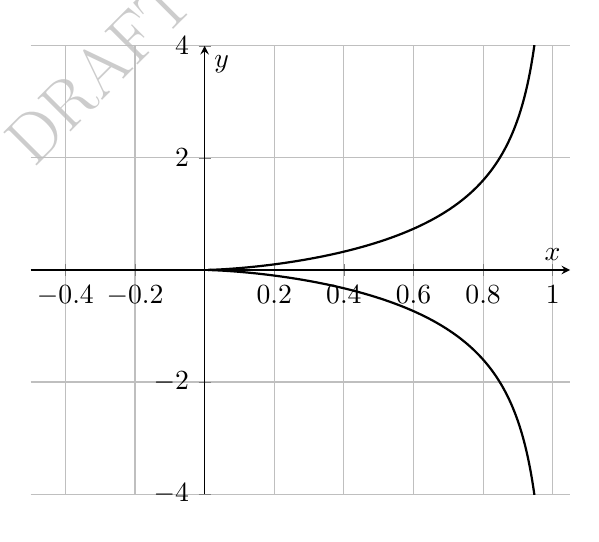
\begin{tikzpicture}
    \begin{axis}[
        axis lines = middle,
        xlabel = $x$,
        ylabel = $y$,
        ymin = -4, ymax = 4,
        xmin = -0.5, xmax = 1.05,
        domain = 0.01:0.99, % Évite les singularités aux limites
        samples = 600,
        legend pos = north west,
        grid = both
    ]
        % Courbe positive
        \addplot[
            color=black,
            thick
        ]{sqrt(x^3/(1-x))};
  %      \addlegendentry{$y = +\sqrt{\frac{x^3}{1-x}}$}
        
        % Courbe négative
        \addplot[
            color=black,
            thick
        ]{-sqrt(x^3/(1-x))};
      %  \addlegendentry{$y = -\sqrt{\frac{x^3}{1-x}}$}
    \end{axis}
\end{tikzpicture}
\end{center}




\quad

\medskip\textbf{Exercice 2} 

Soit $f$ la fonction définie sur $\mathbb{R}_{+}^{*}$ par
 \[
 \begin{cases}
 f(0)=0\\
 f(x)= \frac{x^2}{sh x}
 \end{cases}
 \]
 
 1. Déterminons le développement limité d'ordre 5 de $e^x$ et de $sh x$ en 0.
 
 \[e^x=\sum_{k=0}^n\frac{x^k}{k!}=1+x+\frac{1}{2}x^2+\frac{1}{6}x^3+\frac{1}{24}x^4+\frac{1}{120}x^5 + \circ(x^5)\]
 
 
\[sh x=\sum_{k=0}\frac{x^{2k+1}}{(2k+1)!}=x+\frac{x^3}{6}+\frac{x^5}{120}+\circ(x^5)\] 
 
 2. Déduisons le développement limité d'ordre 3 de $f$ en 0.
 
 \[f(x)=\frac{x^2}{sh x}=\frac{x^2}{x+\frac{x^3}{6}+\frac{x^5}{120}+\circ(x^5)}=\frac{x}{1+\frac{x^2}{6}+\frac{x^4}{120}+\circ(x^4)}=x-\frac{x^3}{6}+\circ(x^3)\](Obtenue par division euclidienne)
 
 3. Déduisons que $f$ est dérivable sur $\mathbb{R}$ et précisons la position relative au voisinage de 0 du graphe de $f$ par rapport à sa tangente en 0.
 
 $f(x)=x-\frac{x^3}{6}+\circ(x^3)$ est un polynôme donc dérivable sur $\mathbb{R}$
 
 Sa tangente en 0 est donnée par $(T): y=x$.
 
 On a : $f(x)-x=-\frac{x^3}{6}+\circ(x^3)\leq 0\forall x\in \mathbb{R}_{+}^{*}$ alors $(C_f)$ est en dessous de $(T)$.
 
 
 4. Déduisons $f^{(3)}(0)$.
 
 \[f'(0)=1 \text{  } , f''(0)= 0 \text{  }, f^{(3)}(0)=-\frac{1}{6}\]
 
 En effet, 
 
 \[f(x)=f(0)+xf'(0)+x^2f''(0)+x^3f^{(3)}(0)=x-\frac{x^3}{6}\]
 
 Par identification, on trouve les résultats ci-dessus.
 

\medskip\textbf{Exercice 3}


1.(a) Le nombre de codes possible :

Chaque chiffre peut être compris entre 1 et 9.

Nombre total de combinaisons : $9\times 9\times 9 =$\textbf{ 729 codes.}

(b) Nombre de codes se terminant par un chiffre impair :

Les chiffres impairs sont : 1,3,5,7,9 (5 possibilités).

Les deux premiers chiffres du code peuvent être quelconque : $9\times 9$.

Ainsi le nombre de codes se terminant par un chiffre impair est : $9\times 9\times 5=405$ codes.

\medskip
Déduisons le nombre de codes se terminant par un chiffres pair :

Par différence, le nombre de codes se terminant par un chiffre pair est :  729-405=\textbf{ 324 codes}.

(c) Nombre de codes contenant au plus un chiffre 5 :

On dénombre ici ou il n'y a aucun chiffre 5 ou il y a exactement un chiffre 5.

$\bullet$ \textbf{Aucun chiffre 5 :} chaque chiffre peut être 1,2,3,4,6,7,8,9 (8 possibilités).

Nombre de codes dans ce cas : $8\times 8\times 8=512$  codes

$\bullet$ \textbf{Exactement un chiffre 5 :} 5 peut être placé à l'une des 3 positions( choix des positions $C_3^1=3$). Les deux autres chiffres sont choisis parmi 1,2,3,4,6,7,8,9 ( 8 possibilités chacun)

Nombre de codes : $3\times 8\times 8 = 192$ codes.

$\quad$

Ainsi le nombre total de codes avec au plus un chiffre 5 est :512+192 codes = \textbf{704 codes}


(d) Le nombre de codes ne contenant pas le chiffre 5.

Tous les chiffres sont choisis parmi 1,2,3,4,6,7,8,9(8 possibilités).

Nombre de codes : $8\times 8\times 8$= \textbf{512 codes}.

\quad

2.(a) Nombre de codes possibles

Les chiffres doivent être distincts :

$\bullet$ \underline{$1^{er}$ chiffre :} 9 choix.

$\bullet$ \underline{$2^{eme}$ chiffre :} 8 choix (différent du premier).

$\bullet$ \underline{$3^{eme}$ chiffre :} 7 choix (différent des deux premiers).

Nombre total des combinaisons possibles : $9\times 8\times 7$= \textbf{504 codes}

(b) Le nombre de codes se terminant par un chiffre pair :

Le dernier chiffre est choisi parmi les chiffres pairs (2,4,6,8) (4 possibilités).

Les deux premiers chiffres sont choisis parmi les 8 chiffres restants de façon distincts : 8 choix pour le premier et 7 choix pour le deuxième.

Nombre de codes : $8\times 7\times 4$=\textbf{224 codes}

\quad

Déduisons le nombre de codes se terminant par un chiffre impair :


Par différence, le nombre de codes se terminant par un chiffre impair est : 504-224 = \textbf{280 codes}


(c) Nombre de codes comprenant les chiffres 5 et 7 :

$\cdot$ Les chiffres 5 et 7 doivent être dans le code.

$\cdot$ Choix des positions des chiffres 5 et 7 dans les trois places : $C_3^2=3$

$\cdot$ Le troisième chiffre est choisi parmi les 7 chiffres restants (distincts de 5 et 7).

Nombre de codes : $3\times 7=$\textbf{ 21 codes}


\quad

\textbf{Exercice 4}

La fonction f est définie sur $\mathbb{R}^2$ par :
\[
f(x, y) = 2x^3 + xy^2 + 5x^2 + y^2.
\]

1. Recherche d'un maximum ou minimum global

Pour déterminer si $f$ possède un maximum ou minimum global sur $\mathbb{R}^2$, nous analysons le comportement de $f(x, y)$ lorsque $\|(x, y)\| \to \infty$.

\[
f(x, y) = 2x^3 + xy^2 + 5x^2 + y^2.
\]

Lorsque $x \to \pm \infty$, le terme dominant est $2x^3$, qui diverge respectivement vers $+\infty$ ou $-\infty$. Donc, $f(x, y)$ ne possède pas de borne supérieure ni de borne inférieure. 

Conclusion : La fonction $f$ n'a pas de maximum ni de minimum global sur $\mathbb{R}^2$.

2. Recherche des extrémums locaux

Pour trouver les points où $f$ présente des extrémums locaux, calculons le gradient de $f$ :
\[
\nabla f(x, y) = \left( \frac{\partial f}{\partial x}, \frac{\partial f}{\partial y} \right).
\]

Les dérivées partielles sont :
\[
\frac{\partial f}{\partial x} = 6x^2 + y^2 + 10x, \quad \frac{\partial f}{\partial y} = 2xy + 2y.
\]

Pour trouver les points critiques, résolvons le système :
\[
\frac{\partial f}{\partial x} = 0 \quad \text{et} \quad \frac{\partial f}{\partial y} = 0.
\]

\textbf{ Résolution du système}

 $\frac{\partial f}{\partial y} = 2y(x + 1) = 0$ \\
   Cette équation donne deux cas :
\[
   y = 0 \quad \text{ou} \quad x = -1.
\]

 Étudions chaque cas :

   - Si $y = 0$, alors $\frac{\partial f}{\partial x} = 6x^2 + 10x = 0$, soit :
\[
     x(6x + 10) = 0 \implies x = 0 \quad \text{ou} \quad x = -\frac{5}{3}.
\]

   - Si $x = -1$, alors $\frac{\partial f}{\partial x} = 6(-1)^2 + y^2 + 10(-1) = y^2 - 4 = 0$, soit :
\[
     y^2 = 4 \implies y = \pm 2.
\]

$\cdot$ \textbf{Points critiques}

Les points critiques de $f$ sont donc :
\[
(0, 0), \quad \left(-\frac{5}{3}, 0\right), \quad (-1, 2), \quad (-1, -2).
\]

$\cdot$ \textbf{ Nature des points critiques}

Pour déterminer la nature des points critiques (minimum local, maximum local ou point selle), calculons la matrice hessienne de $f$ :
\[
H_f(x, y) = 
\begin{pmatrix}
\frac{\partial^2 f}{\partial x^2} & \frac{\partial^2 f}{\partial x \partial y} \\
\frac{\partial^2 f}{\partial y \partial x} & \frac{\partial^2 f}{\partial y^2}
\end{pmatrix}.
\]

Les dérivées secondes sont :
\[
\frac{\partial^2 f}{\partial x^2} = 12x + 10, \quad 
\frac{\partial^2 f}{\partial y^2} = 2x + 2, \quad 
\frac{\partial^2 f}{\partial x \partial y} = \frac{\partial^2 f}{\partial y \partial x} = 2y.
\]

La matrice hessienne est donc :
\[
H_f(x, y) = 
\begin{pmatrix}
12x + 10 & 2y \\
2y & 2x + 2
\end{pmatrix}.
\]

$\cdot$ Étudions la nature des points critiques :

- Point $(0, 0)$ :
\[
   H_f(0, 0) = 
   \begin{pmatrix}
   10 & 0 \\
   0 & 2
   \end{pmatrix}.
\]

   Les valeurs propres sont $10 > 0$ et $2 > 0$. Donc, $(0, 0)$ est un \textbf{minimum local}.

- Point $\left(-\frac{5}{3}, 0\right)$ :
\[
   H_f\left(-\frac{5}{3}, 0\right) = 
   \begin{pmatrix}
   12\left(-\frac{5}{3}\right) + 10 & 0 \\
   0 & 2\left(-\frac{5}{3}\right) + 2
   \end{pmatrix} = 
   \begin{pmatrix}
   0 & 0 \\
   0 & -\frac{4}{3}
   \end{pmatrix}.
\]

   La matrice n'est pas définie, donc $\left(-\frac{5}{3}, 0\right)$ est un \textbf{point selle}.

- Point $(-1, 2)$ :
\[
   H_f(-1, 2) = 
   \begin{pmatrix}
   12(-1) + 10 & 4 \\
   4 & 2(-1) + 2
   \end{pmatrix} = 
   \begin{pmatrix}
   -2 & 4 \\
   4 & 0
   \end{pmatrix}.
\]

   Le déterminant est $\det(H_f(-1, 2)) = (-2)(0) - (4)(4) = -16 < 0$. Donc, $(-1, 2)$ est un \textbf{point selle}.

- Point $(-1, -2)$ :*
\[
   H_f(-1, -2) = 
   \begin{pmatrix}
   -2 & -4 \\
   -4 & 0
   \end{pmatrix}.
\]

   Le déterminant est $\det(H_f(-1, -2)) = -16 < 0$. Donc, $(-1, -2)$ est un \textbf{point selle}.
   
   \medskip

\textbf{ Conclusion}

- $(0, 0)$ est un \textbf{minimum local}.
- $\left(-\frac{5}{3}, 0\right), (-1, 2), (-1, -2)$ sont des \textbf{points selle}.







\medskip\textbf{Sujet 8}

\textbf{Exercice 1}

1.a) Soit $\overrightarrow{U}=(x,y,z)^T\in \mathbb{R}^3$. On a :

$T(\overrightarrow{U})=T(xe_1+ye_2+ze_3)=xe_3+y(-e_1+e_2+e_3)+ze_3=-ye_1+ye_2+(x+y+z)e_3$.

Ainsi, 

$\overrightarrow{U}=\begin{pmatrix}
x\\
y\\
z\\
\end{pmatrix}\in Ker(T)\Longleftrightarrow \begin{cases}
y=0\\
x+y+z=0
\end{cases}\Longleftrightarrow \begin{cases}
x=k_1, k_1\in \mathbb{R}\\
y=0\\
z=-k_1
\end{cases}\Longleftrightarrow \overrightarrow{U}=k_1\begin{pmatrix}
1\\
0\\
-1
\end{pmatrix}, k_1\in \mathbb{R}$ et $Ker(T)=Vect\langle \begin{pmatrix}
1\\
0\\
-1
\end{pmatrix}\rangle$.


b)  Pour écrire la matrice de l'application linéaire $T$ dans la base $B$ on calcul $T(e_1),
 T(e_2)$ et $T(e_3)$ que l'on exprime dans la base $B$ puis on concatène ces vecteurs pour former $A$.Les vecteurs $T(e_i),(i=1,2,3)$ étant donnés dans l'énoncé on a directement :
 
 $A=\begin{pmatrix}
 0 & -1 & 0 \\ 
 0 & 1 & 0 \\ 
 1 & 1 & 1.
 \end{pmatrix}$
 
 2.a) On a 
 $
 \begin{cases}
 f_1=e_1-e_3\\
 f_2=e_1-e_2\\
 f_3=-e_1+e_2+e_3
 \end{cases}\Leftrightarrow \begin{cases}
 e_3=e_1-f_1=f_2+f_3\\
 e_1=f_2+e_2=f_1+f_2+f_3\\
 e_2=f_1+f_3 (L_3\longleftarrow L3+L1)
 \end{cases}
 $
 
 Ainsi $\mathbb{R}^3=Vect\langle e_1,e_2,e_3\rangle\subset Vect\langle f_1,f_2,f_3\rangle$. La famille $(f_1,f_2,f_3)$ est donc génératrice minimale et c'est une base.
 
 b) On a :
 
 $
 T(f_1)=\begin{pmatrix}
 0 & -1 & 0 \\ 
 0 & 1 & 0 \\ 
 1 & 1 & 1.
 \end{pmatrix}\begin{pmatrix}
1\\
0\\
-1
\end{pmatrix}=0_{\mathbb{R}^3}
$ en remarquant que $f_1\in Ker(T)$

$
T(f_2)=\begin{pmatrix}
 0 & -1 & 0 \\ 
 0 & 1 & 0 \\ 
 1 & 1 & 1.
 \end{pmatrix}\begin{pmatrix}
1\\
-1\\
0
\end{pmatrix}=\begin{pmatrix}
1\\
-1\\
0
\end{pmatrix}=f_2,
$

$
T(f_3)=\begin{pmatrix}
 0 & -1 & 0 \\ 
 0 & 1 & 0 \\ 
 1 & 1 & 1.
 \end{pmatrix}\begin{pmatrix}
-1\\
1\\
1
\end{pmatrix}=\begin{pmatrix}
-1\\
1\\
1
\end{pmatrix}=f_3
$

Ainsi la matrice $B$ de $T$ dans la base $(f_1,f_2,f_3)$ est donnée par :

$
B=\begin{pmatrix}
 0 & 0 & 0 \\ 
 0 & 1 & 0 \\ 
 0 & 0 & 1.
 \end{pmatrix}
 $
 
 3. On va vérifier que $P$ est inversible et calculer $P^{-1}$ en même temps. $P$ est inversible si et seulement si,pour tout $Y\in \mathbb{R}^3$, il existe un unique $X\in \mathbb{R}^3$ tel que $PX=Y$. On fixe donc $Y=(y_1,y_2,y_3)^T\in \mathbb{R}^3$ et on résout le système : 
 
 $
 \begin{cases}
 x_1+x_2-x_3=y_1\\
 -x_2+x_3=y_2\\
 -x_1+x_3=y_3
 \end{cases}\Leftrightarrow \begin{cases}
 x_2=y_1+y_3 (L_1\longleftarrow L_1+L3)\\
 x_3=y_1+y_2+y_3\\
 x_1=y_1+y_2
 \end{cases}
 $
 
  Le système précédent admet donc une unique solution,$P$ est inversible et $P^{-1}$ est donnée par :
  
  $
  \begin{pmatrix}
 1 & 1 & 0 \\ 
 1 & 0 & 1 \\ 
 1 & 1 & 1.
 \end{pmatrix} \hspace*{1cm}\begin{cases}
 x_1=\textbf{1} y_1+\textbf{1}y_2+\textbf{0}y_3\\
 x_2=\textbf{1} y_1+\textbf{0}y_2+\textbf{1}y_3\\
 x_3=\textbf{1} y_1+\textbf{1}y_2+\textbf{1}y_3
 \end{cases}
 $
 
  \textbf{Deuxième méthode} : $P$ est la matrice de passage de la base $B$ à la base $V$, elle est
 donc inversible. La matrice $P^{-1}$ est la matrice de passage de la base $V$ à la base $B$. Pour
 écrire cette matrice on utilise la relation (obtenue précédemment dans l'exercice) :
 
 $
 \begin{cases}
 e_1=f_1+f_2+y_3\\
 e_2=f_1+f_3\\
 e_3=f_2+f_3
\end{cases}
 $
 
 Cela nous donne directement $P^{-1}$ en concaténant les $e_i$ exprimés en fonction des $f_i$.
Finalement la formule du changement de base sur les matrices donne:

$
A=PBP^{-1}
$

\underline{\textbf{Rappel :}}

 Soit $f :E\rightarrow E$ une application linéaire. Soit $B$ et $B'$ deux bases de $E$. On note $A$
 (respectivement $B$) la matrice de $f$ dans la base $B$ (respectivement $B'$). Soit $u$ un vecteur
 de $E$. Soit $X$ le vecteur colonne associé à $u$ dans la base $B$  et $Y$ le vecteur colonne associé
 à $u$ dans la base $B'$. On a la relation $X=PY$ avec $P$ la matrice de passage de $B$ à $B'$.
 
 Si on calcul $f(u)$ et que l'on exprime le résultat dans la base $B$ on a:
 
$ [f(u)]_B=AX$

 Calculons maintenant $f(u)$ en passant par la base $B'$. On a
$ [f(u)]_{B^{'}}=BY$
 
  On passe d'une expression à l'autre en utilisant la matrice de passage $P$ donc:

$ [f(u)]_B=P[f(u)]_{B^{'}}$

Soit $AX=PBY$, mais $Y=P^{-1}X$ donc finalement : 

$AX=PBP^{-1}X$.

Cette relation implique donc l'égalité matricielle $A=PBP^{-1}$.






\medskip\textbf{Exercice 2} 

Le plan $(P)$ est rapporté à un repère orthonormé direct $(\overrightarrow{0} ; \overrightarrow{u}; \overrightarrow{v})$. On désigne par \(T\) l'application de \((P)\) dans \((P)\) qui, à tout point \(M\) d'affixe \(z\), associe le point \(M'\) d'affixe : 
\[
z' = (1+i)z - i.
\]

\medskip
\textbf{1. Décomposition de \(T\) en une rotation et une homothétie}

\begin{itemize}
    \item On écrit \(z' = (1+i)z - i = \sqrt{2}e^{i\pi/4}z - i\).
    \item L'application \(T\) est donc une homothétie de rapport \(k = |1+i| = \sqrt{2}\) suivie d'une rotation d'angle \(\theta = \frac{\pi}{4}\), le tout combiné avec une translation de vecteur \(-i\).
    \item Le point invariant par \(T\) (point fixe) est obtenu en résolvant \(z' = z\), soit :
    \[
    z = \sqrt{2}e^{i\pi/4}z - i \implies z(1 - \sqrt{2}e^{i\pi/4}) = -i \implies z = \frac{-i}{1 - \sqrt{2}e^{i\pi/4}}.
    \]
    \item Simplifions : \(z = \Omega = \frac{-i(1 - \sqrt{2}e^{-i\pi/4})}{(1 - \sqrt{2}e^{i\pi/4})(1 - \sqrt{2}e^{-i\pi/4})} = -1 - i\).
    \item Le point invariant \(\Omega\) a donc pour affixe \(z_\Omega = -1 - i\).
    \item L'angle orienté \((\overrightarrow{\Omega M}, \overrightarrow{MM'})\), pour \(M \neq \Omega\), est \(\theta = \frac{\pi}{4}\).
\end{itemize}

\medskip
\textbf{2.a) Construction de \(M'\), image de \(M\) par \(T\)}

Soit \(M\) un point donné d'affixe \(z\), l'affixe de \(M'\) est :
\[
z' = \sqrt{2}e^{i\pi/4}z - i.
\]
Pour tracer \(M'\), on applique successivement :
\begin{itemize}
    \item une homothétie de rapport \(\sqrt{2}\),
    \item une rotation d'angle \(\frac{\pi}{4}\),
    \item une translation de vecteur \(-i\).
\end{itemize}

\textbf{2.b) Image de la droite \((D)\) par \(T\)}

La droite \((D)\) a pour équation \(y = x\), soit \(z = x + ix\). On a donc :
\[
z' = (1+i)z - i = (1+i)(x + ix) - i = (1 - x) + i(2x - 1).
\]
Les affixes \(z'\) des points de \((D')\) satisfont l'équation :
\[
x' = 1 - y', \quad \text{soit } y' = -x' + 1.
\]
La droite \((D')\) a donc pour équation \(y = -x + 1\).

\medskip
\textbf{3.a) Existence et unicité de \(B\)}

On cherche un point \(B\) distinct de \(\Omega\) tel que \(z_0z'_0 = 1\), avec \(z'_0 = (1+i)z_0 - i\). On a donc :
\[
z_0 \big((1+i)z_0 - i\big) = 1 \implies z_0^2(1+i) - iz_0 - 1 = 0.
\]
Posons \(z_0 = x + iy\) (où \(x, y \in \mathbb{R}\)) et résolvons cette équation complexe pour trouver \(z_0\). 

Le calcul donne \(z_0 = \frac{1 + i}{2}\). Le point \(B'\), image de \(B\), est alors \(z'_0 = \frac{2}{1+i} = 1 - i\).

\medskip
3.b) Cocyclicité des points \(\Omega', \Omega, B, B'\)

Le point \(\Omega'\), symétrique de \(\Omega\) par rapport à \(O\), a pour affixe \(z_{\Omega'} = 1 + i\).

Les points \(\Omega', \Omega, B, B'\) sont cocycliques si leurs affixes satisfont la relation de cercle. On montre que le centre \(G\) de ce cercle a pour affixe :
\[
z_G = \frac{z_\Omega + z_{\Omega'} + z_B + z_{B'}}{4} = \frac{(-1-i) + (1+i) + \frac{1+i}{2} + (1-i)}{4}.
\]
Le calcul donne \(z_G = \frac{1}{2}\).

Ainsi, le centre du cercle est \(G\) d'affixe \(z_G = \frac{1}{2}\).









\begin{center}
\textbf{Constructions Géométriques}


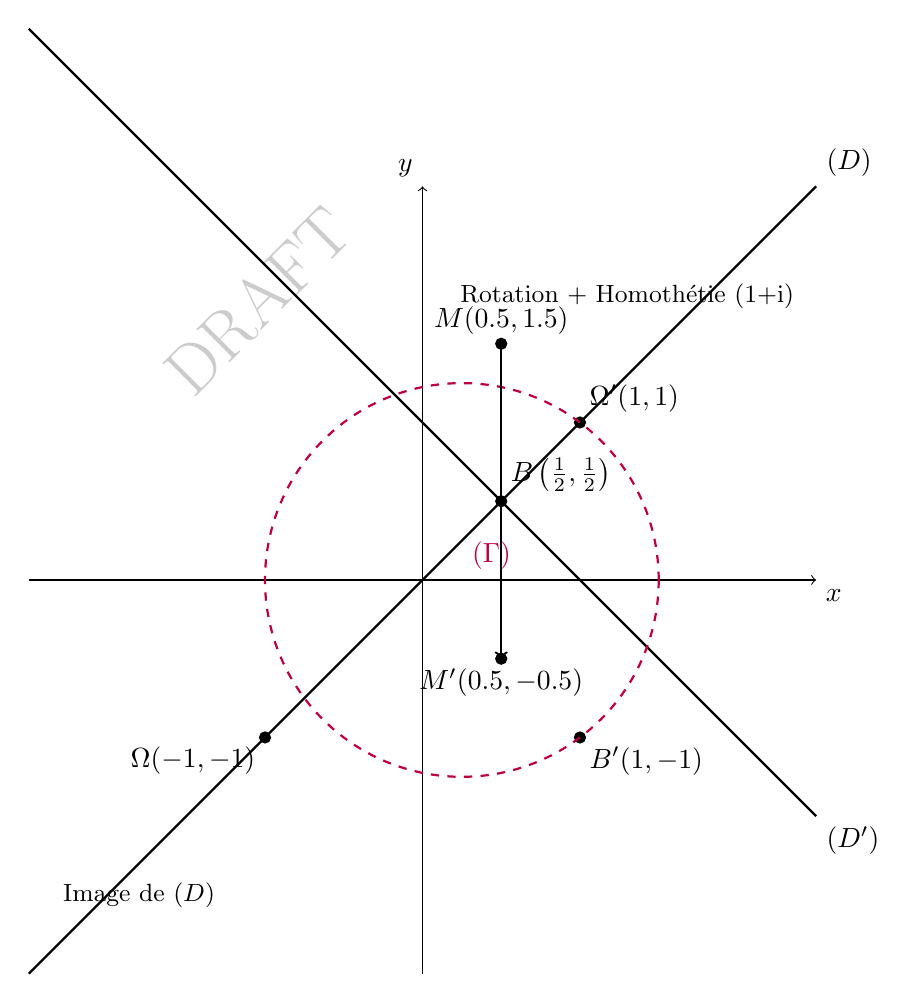
\begin{tikzpicture}[scale=2]
    % Repère orthonormé
    \draw[->] (-2.5, 0) -- (2.5, 0) node[anchor=north west] {$x$};
    \draw[->] (0, -2.5) -- (0, 2.5) node[anchor=south east] {$y$};
    \draw[thick] (-2.5, -2.5) -- (2.5, 2.5) node[above right] {$(D)$};
    \draw[thick, black] (-2.5, 3.5) -- (2.5, -1.5) node[below right] {$(D')$};
    
    % Points principaux
    \filldraw[black] (-1,-1) circle (1pt) node[below left] {$\Omega(-1, -1)$};
    \filldraw[black] (1,1) circle (1pt) node[above right] {$\Omega'(1, 1)$};
    \filldraw[black] (0.5, 0.5) circle (1pt) node[above right] {$B\left(\frac{1}{2}, \frac{1}{2}\right)$};
    \filldraw[black] (1,-1) circle (1pt) node[below right] {$B'(1, -1)$};
    
    % Cercle passant par Omega, Omega', B et B'
    \draw[thick, dashed, purple] (0.25,0) circle (1.25) node[above right] {$(\Gamma)$};
    
    % Exemple point M et son image M'
    \filldraw[black] (0.5, 1.5) circle (1pt) node[above] {$M(0.5, 1.5)$};
    \filldraw[black] (0.5, -0.5) circle (1pt) node[below] {$M'(0.5, -0.5)$};
    \draw[->, thick, black] (0.5, 1.5) -- (0.5, -0.5);

    % Légendes et étiquettes
    \node at (1.3, 1.8) [black] {\small Rotation + Homothétie (1+i)};
    \node at (-1.8, -2) [black] {\small Image de $(D)$};
\end{tikzpicture}
\end{center}

\quad



\medskip\textbf{Exercice 3}


1. Calculons

$I=\int\int_D\frac{dxdy}{(1+x^2+y^2)^2}$ ou $D=\lbrace {(x,y) \in \mathbb{R}^2,\vert x\vert \leq x^2+y^2\leq 1\rbrace}$.

Passage aux coordonnées polaires :

Soit $x=r\cos \theta$ et $y=r\sin\theta$

$x^2+y^2=r^2$

$x^2+y^2\leq 1\Rightarrow r^2\leq 1\Rightarrow 0\leq r\leq 1$

$\vert x\vert \leq x^2+y^2\Rightarrow \theta\in [0,2\pi]$

A travers le jacobien, $dxdy=rdrd\theta$

Donc,

$I=\int_0^1\int_0^{2\pi}\frac{rdrd\theta}{(1+r^2)^2}=\int_0^{2\pi}d\theta\times\int_0^1\frac{rdr}{(1+r^2)^2}=2\pi\int_0^1\frac{rdr}{(1+r^2)^2}$

Posons $u=1+r^2$, $du=2rdr\Longrightarrow dr=\frac{du}{2r}$

Si $r\to 0$, $u\to 1$ et si  $r\to 1$, $u\to 2$

L'intégrale devient :

$I=2\pi\times\frac{1}{2}\int_1^2\frac{du}{u^2}=\pi[-\frac{1}{u}]_1^2=\pi(-\frac{1}{2}+1)=\frac{\pi}{2}$


2. Calculons l'intégrale double

$J=\int\int_D(x+y)^2dxdy$ ou $D=\lbrace (x,y)\in \mathbb{R}^2, x^2+y^2-x \leq 0;x^2+y^2-y \geq 0$ et $y \geq 0 \rbrace$.

 Définition et analyse de la région \(D\)
 
La région \(D\) est définie par trois inégalités :
\begin{itemize}
    \item \( x^2 + y^2 - x \leq 0 \), ce qui correspond au disque de centre \(\left( \frac{1}{2}, 0 \right)\) et de rayon \(\frac{1}{2}\).
    \item \( x^2 + y^2 - y \geq 0 \), ce qui correspond à l'extérieur du disque de centre \((0, \frac{1}{2})\) et de rayon \(\frac{1}{2}\).
    \item \( y \geq 0 \), restreignant la région au demi-plan supérieur.
\end{itemize}

\textbf{Intersection :} La région \(D\) est l'intersection du disque centré en \(\left( \frac{1}{2}, 0 \right)\) avec l'extérieur du disque centré en \((0, \frac{1}{2})\), dans le demi-plan supérieur. Les frontières des disques peuvent être exprimées en coordonnées polaires :
\begin{itemize}
    \item \( (x - \frac{1}{2})^2 + y^2 = \frac{1}{4} \Rightarrow r = \cos\theta \),
    \item \( x^2 + (y - \frac{1}{2})^2 = \frac{1}{4} \Rightarrow r = \sin\theta \).
\end{itemize}
La région \(D\) en polaires est donc donnée par :
\[ \theta \in [0, \frac{\pi}{2}], \quad r \in [\sin\theta, \cos\theta]. \]

 Réécriture de l'intégrale en coordonnées polaires
 
En polaires :

\begin{align*}
    x &= r\cos\theta, \quad y = r\sin\theta, \quad x + y = r(\cos\theta + \sin\theta), \\
    dxdy &= r drd\theta.
\end{align*}
L'intégrale devient :
\[
    J = \int_0^{\pi/2} \int_{\sin\theta}^{\cos\theta} \left[r(\cos\theta + \sin\theta)\right]^2 r \, dr \, d\theta.
\]

Développons \((\cos\theta + \sin\theta)^2\) :
\[
    (\cos\theta + \sin\theta)^2 = \cos^2\theta + 2\cos\theta\sin\theta + \sin^2\theta = 1 + 2\cos\theta\sin\theta.
\]
Ainsi :
\[
    J = \int_0^{\pi/2} \int_{\sin\theta}^{\cos\theta} r^3 \left(1 + 2\cos\theta\sin\theta\right) \, dr \, d\theta.
\]

\textbf{Calcul de l'intégrale}

 Intégration par rapport à \(r\)
 
\[
    \int_{\sin\theta}^{\cos\theta} r^3 \, dr = \left[ \frac{r^4}{4} \right]_{\sin\theta}^{\cos\theta} = \frac{\cos^4\theta}{4} - \frac{\sin^4\theta}{4}.
\]
Substituons dans \(J\) :
\[
    J = \int_0^{\pi/2} \left[ \frac{\cos^4\theta}{4} - \frac{\sin^4\theta}{4} \right] \left(1 + 2\cos\theta\sin\theta\right) d\theta.
\]

 Séparation des termes
 
Développons :
\begin{align*}
    J &= \frac{1}{4} \int_0^{\pi/2} \cos^4\theta (1 + 2\cos\theta\sin\theta) \, d\theta - \frac{1}{4} \int_0^{\pi/2} \sin^4\theta (1 + 2\cos\theta\sin\theta) \, d\theta. \\
    &= \frac{1}{4} \left[ \int_0^{\pi/2} \cos^4\theta \, d\theta + 2 \int_0^{\pi/2} \cos^5\theta\sin\theta \, d\theta \right] \\
    &\quad - \frac{1}{4} \left[ \int_0^{\pi/2} \sin^4\theta \, d\theta + 2 \int_0^{\pi/2} \cos\theta\sin^5\theta \, d\theta \right].
\end{align*}

 Calcul des intégrales élémentaires
 
 \(\int_0^{\pi/2} \cos^4\theta \, d\theta\) et \(\int_0^{\pi/2} \sin^4\theta \, d\theta\) : Utilisons les formules de réduction :
\[
    \int_0^{\pi/2} \cos^4\theta \, d\theta = \int_0^{\pi/2} \sin^4\theta \, d\theta = \frac{3\pi}{16}.
\]

 \(\int_0^{\pi/2} \cos^5\theta\sin\theta \, d\theta\) et \(\int_0^{\pi/2} \cos\theta\sin^5\theta \, d\theta\) : Par substitution \(u = \cos\theta\) ou \(u = \sin\theta\), on trouve :
\[
    \int_0^{\pi/2} \cos^5\theta\sin\theta \, d\theta = \int_0^{\pi/2} \cos\theta\sin^5\theta \, d\theta = \frac{1}{6}.
\]

Résultat final

En combinant tous les termes :
\[
    J = \frac{1}{4} \left[ \frac{3\pi}{16} + 2 \cdot \frac{1}{6} \right] - \frac{1}{4} \left[ \frac{3\pi}{16} + 2 \cdot \frac{1}{6} \right] = \frac{1}{15}.
\]

\textbf{Ainsi, la valeur de l'intégrale est :}
\[
    J = \frac{1}{15}.
\]




3. Soit $D=\lbrace (x,y,z)\in \mathbb{R}^3;x\geq 0,y\geq 0,z\geq 0,x+y+z\leq 1 \rbrace$.

Utilisons le changement de variable $u=x+y+z; v=\frac{z}{y+z}; w=\frac{y+z}{x+y+z}$ pour calculer

$S=\int\int_D\frac{z^3}{(x+y+z)(y+z)}dxdydz$.

On effectue le changement de variables suivant :
\[
u = x + y + z, \quad v = \frac{z}{y + z}, \quad w = \frac{y + z}{x + y + z}.
\]

 Jacobien du changement de variables

Pour déterminer le jacobien de ce changement de variables, nous devons calculer le déterminant de la matrice des dérivées partielles des nouvelles variables \( u, v, w \) par rapport aux anciennes variables \( x, y, z \). Le jacobien \( J \) est donné par :
\[
J = \det \begin{pmatrix} 
\frac{\partial u}{\partial x} & \frac{\partial u}{\partial y} & \frac{\partial u}{\partial z} \\
\frac{\partial v}{\partial x} & \frac{\partial v}{\partial y} & \frac{\partial v}{\partial z} \\
\frac{\partial w}{\partial x} & \frac{\partial w}{\partial y} & \frac{\partial w}{\partial z}
\end{pmatrix}.
\]

Cela peut être calculé en effectuant les dérivées partielles de chaque variable par rapport à \( x \), \( y \), et \( z \), et en déterminant le déterminant de la matrice résultante.

 L'intégrale après changement de variables

L'intégrale que nous devons calculer est :
\[
S = \int \int \int_D \frac{z^3}{(x + y + z)(y + z)} \, dx \, dy \, dz.
\]

Après le changement de variables, l'intégrale devient :
\[
S = \int_0^1 \int_0^1 \int_0^1 \frac{u^3 v^3}{u^3 v} \cdot J \, du \, dv \, dw,
\]
où \( J \) est le jacobien du changement de variables.

 Simplification de l'intégrale

Simplifions l'expression de l'intégrale :
\[
S = \int_0^1 \int_0^1 \int_0^1 u^2 v^2 \, du \, dv \, dw.
\]

Cela donne une intégrale séparée, et les intégrales sur \( u \), \( v \), et \( w \) peuvent être calculées indépendamment :
\[
\int_0^1 u^2 \, du = \frac{1}{3}, \quad \int_0^1 v^2 \, dv = \frac{1}{3}, \quad \int_0^1 1 \, dw = 1.
\]

 Conclusion

En multipliant ces résultats, nous obtenons :
\[
S = \frac{1}{3} \cdot \frac{1}{3} \cdot 1 = \frac{1}{9}.
\]

Ainsi, l'intégrale \( S \) est égale à \( \frac{1}{9} \)


4. Calculons l'aire du domaine elliptique :

$E = \lbrace (x,y)\in \mathbb{R}^2;\frac{x^2}{a^2}+\frac{y^2}{b^2}\leq 1\rbrace$.

Il s'agit d'une ellipse centrée en \( (0, 0) \), avec des axes de longueurs \( 2a \) et \( 2b \) dans les directions \( x \) et \( y \), respectivement.

 Changement de variables

Pour calculer l'aire de l'ellipse, nous utilisons un changement de variables pour transformer l'ellipse en un cercle unité. On définit les nouvelles variables \( u \) et \( v \) par :
\[
u = \frac{x}{a}, \quad v = \frac{y}{b}.
\]

Ainsi, l'ellipse devient l'ensemble des points \( (u, v) \) satisfaisant :
\[
u^2 + v^2 \leq 1,
\]
c'est-à-dire un disque de rayon 1 centré en \( (0, 0) \).

Jacobien du changement de variables

Le jacobien du changement de variables \( (x, y) \mapsto (u, v) \) est donné par le déterminant de la matrice des dérivées partielles :
\[
J = \det \begin{pmatrix} \frac{\partial u}{\partial x} & \frac{\partial u}{\partial y} \\ \frac{\partial v}{\partial x} & \frac{\partial v}{\partial y} \end{pmatrix}
= \det \begin{pmatrix} \frac{1}{a} & 0 \\ 0 & \frac{1}{b} \end{pmatrix}
= \frac{1}{ab}.
\]

Le facteur de transformation de l'aire est donc \( \frac{1}{ab} \).

 Aire du domaine elliptique

L'aire du domaine \( E \) dans le plan \( (x, y) \) est égale à l'aire du disque unité dans le plan \( (u, v) \) multipliée par le facteur de transformation \( \frac{1}{ab} \). L'aire du disque unité est \( \pi \), donc l'aire de \( E \) est :
\[
\text{Aire}(E) = \pi \cdot a \cdot b.
\]

Conclusion

L'aire du domaine elliptique \( E \) est donnée par :
\[
\text{Aire}(E) = \pi \cdot a \cdot b.
\]





\medskip\textbf{Exercice 4}


On pose $f(n)=\int_{0}^{1}x^ne^{-x}dx$  $\forall n\in \mathbb{N}$.

1. Montrons que la suite $(f(n))$ est positive et décroissante.

$\forall x\in [0,1]$, $x^ne^{-x}>0$ donc $\int_{0}^{1}x^ne^{-x}dx>0$ d'où $f(n)>0$.

$\forall x\in [0,1]$, $0\leq x\leq 1\Rightarrow 0\leq x^{n+1}\leq x^n$

Donc $\int_{0}^{1}x^{n+1}e^{-x}dx\leq \int_{0}^{1}x^ne^{-x}dx$. Autrement dit $f(n+1)\leq f(n)$, ainsi cette suite est décroissante.

\medskip
Donnons une relation de récurrence entre $f(n)$ et $f(n-1)$.
 
 $f(n)=\int_{0}^{1}x^ne^{-x}dx$
 
 Posons 
 

$ u =x^n\longrightarrow u'=nx^{n-1}\\
 v' =e^{-x}\longrightarrow v=-e^{-x}
$ 
 
 $\Rightarrow f(n)=[-x^ne^{-x}]_0^1+\int_{0}^{1}nx^{n-1}e^{-x}dx$ avec $[-x^ne^{-x}]_0^1=-e^{-1}=-\frac{1}{e}$ et $\int_{0}^{1}nx^{n-1}e^{-x}dx=nf(n-1)$
 
 $\Rightarrow f(n)=-\frac{1}{e}+nf(n-1)$.
 
 
 2. Montrons par récurrence que pour tout $n\in \mathbb{N}$, $f(n)= \frac{n!}{e}(e-\sum_{k=0}^{n}\frac{1}{k!})$
 
 Pour $n=0$, $\int_{0}^{1}x^{0}e^{-x}dx=[-e^{-x}]_0^1=-\frac{1}{e}+1$
 
 On a : $\frac{0!}{e}(e-\sum_{k=0}^{0}\frac{1}{k!})=\frac{1}{e}(e-1)=1-\frac{1}{e}$
 
 Les deux sont égaux, alors l'hypothèse est vérifié au rang 0.
 
 Supposons l'hypothèse vrai à l'ordre $n-1$,c'est-à-dire $f(n-1)= \frac{(n-1)!}{e}(e-\sum_{k=0}^{n-1}\frac{1}{k!})$ et vérifions au rang $n$.
 
 \begin{align*}
f(n) &= -\frac{1}{e} + n f(n-1) \\
     &= -\frac{1}{e} + n \frac{(n-1)!}{e} \left( e - \sum_{k=0}^{n-1} \frac{1}{k!} \right) \\
     \text{avec } n(n-1)! = n! \\
     &= -\frac{1}{e} + \frac{n!}{e} \left( e - \sum_{k=0}^{n-1} \frac{1}{k!} \right) \\
     &= -\frac{n!}{n!e} + \frac{n!}{e} \left( e - \sum_{k=0}^{n-1} \frac{1}{k!} \right) \\
     &= \frac{n!}{e} \left( -\frac{1}{n!} + e - \sum_{k=0}^{n-1} \frac{1}{k!} \right) \\
     \text{avec } -\frac{1}{n!} - \sum_{k=0}^{n-1} \frac{1}{k!} &= -\sum_{k=0}^{n} \frac{1}{k!} \\
f(n) &= \frac{n!}{e} \left( e - \sum_{k=0}^{n} \frac{1}{k!} \right)
\end{align*}

 
 L'hypothèse est donc vrai pour tout $n$. Ce qui achève la récurrence.
 
 3. Montrons que l'on a $\frac{1}{e(n+1)}\leq f(n)\leq \frac{1}{n+1}$.
 
 On a :
 

\begin{align*}
0 \leq x \leq 1 &\Rightarrow -1 \leq -x \leq 0 \\
&\Rightarrow e^{-1} \leq e^{-x} \leq e^{0} \\
&\Rightarrow \frac{1}{e} \times x^n \leq x^n e^{-x} \leq x^n \\
&\Rightarrow \frac{1}{e} \int_{0}^{1} x^n \, dx \leq\int_{0}^{1} x^n e^{-x} \, dx \leq \\
\int_{0}^{1} x^n \, dx \\
\text{avec } \int_{0}^{1} x^n e^{-x} \, dx = f(n) \text{ et } \int_{0}^{1} x^n \, dx = \left[ \frac{1}{n+1} x^{n+1} \right]_{0}^{1} = \frac{1}{n+1} \\
&\Rightarrow \frac{1}{e(n+1)} \leq f(n) \leq \frac{1}{n+1}
\end{align*}

 d'où le résultat
 
 4. Déduisons la nature des séries $\sum_{n=1}^{+\infty}f(n)$, $\sum_{n=1}^{+\infty}\frac{f(n)}{n}$ et $\sum_{n=1}^{+\infty}(-1)^nf(n)$.
 
 On a : $\frac{1}{e(n+1)}\leq f(n)\leq \frac{1}{n+1}$
 
 
 \medskip
 $\bullet \sum_{n=1}^{+\infty}f(n)$

$f(n)$ est minorée par $\frac{1}{e(n+1)}\sim \frac{1}{en}$  qui est le terme général d'une série de Riemann divergente donc la série de terme général $f(n)$, c'est-à-dire $\sum_{n=1}^{+\infty}f(n)$ diverge.
 
 \medskip
 $\bullet \sum_{n=1}^{+\infty}\frac{f(n)}{n}$
 
 $\frac{1}{e(n+1)}\leq f(n)\leq \frac{1}{n+1}\Rightarrow \frac{1}{en(n+1)}\leq \frac{f(n)}{n}\leq \frac{1}{n(n+1)}$
 
 $\frac{f(n)}{n}$ est majorée par $\frac{1}{n(n+1)}\sim \frac{1}{n^2}$ qui est le terme générale d'une série de Riemann convergente donc la série de terme général $\frac{f(n)}{n}$ converge.
 
 $\bullet \sum_{n=1}^{+\infty}(-1)^nf(n)$
 
 $f(n)$ est positive et décroissante, donc la série de terme général $(-1)^nf(n)$ est une série alternée convergente.
 
 
 5. Déterminons le rayon de convergence de la série entière $\sum_{n=1}^{+\infty}f(n)x^n$.

 Soit $R$ le rayon de convergence de la série entière. Comme la série de terme général $f(n)$ diverge cela signifie que 1  n'est pas dans le disque de convergence sinon
$\sum_{n=1}^{+\infty}f(n)1^n=\sum_{n=1}^{+\infty}f(n)$ convergerait, cela entraine que $R\geq 1$.

Comme la série de terme général $(-1)^nf(n)$ converge, cela signifie que -1 est dans le disque de 
converge donc $R\leq 1$ , en effet

$\sum_{n=1}^{+\infty}f(n)(-1)^n< +\infty$

Donc $R=1$


\medskip\textbf{Sujet 9}

\textbf{Exercice 1}

1. Calcul de l'aire de D

On a :

$Aire(D)=\int_{y=0}^2(\int_{x=\frac{y^2}{4}}^{\frac{y}{2}}1dx)dy=\int_0^2(\frac{y}{2}-\frac{y^2}{4})dy=[\frac{y^2}{4}-\frac{y^3}{12}]_0^2=\frac{1}{3}$

2. Calculer l'intégrale

$\int\int_D(y-x)dxdy=\int_{x=0}^{1}(\int_{y=2x}^{2\sqrt{x}}(y-x)dy)dx=\int_{0}^{1}(2x-2x^{\frac{3}{2}})dx=\frac{1}{5}$.

 Pour ces deux calculs il était possible d'intégrer d'abord en $x$ ou en $y$.
 
 3. Calcul de $\int_Cy^2dx+xydy$
 
 a) Directement
 
 On définie le paramètre $C$ par :
 
 $\gamma_1 : \begin{cases}
 [0,1]\rightarrow \mathbb{R}^2\\
 t\mapsto (t,2t)
 \end{cases}$ et $\gamma_2 : \begin{cases}
 [0,1]\rightarrow \mathbb{R}^2\\
 t\mapsto (t,2\sqrt{t})
 \end{cases}$.
 
 On a alors :
 
 $\int_Cy^2dx+xydy=\int_{\gamma_1}y^2dx+xydy-\int_{\gamma_2}y^2dx+xydy=\int_0^1(4t^2+4t^2)dt-\int_0^1(4t+2t)dt=\frac{8}{3}-3=-\frac{1}{3}$.
 
b) D'après la formule de Green-Riemann, on a :
La formule de Green-Riemann s'\'ecrit :
\[
\int_C y^2 dx + xy dy = \int\int_D \left( \frac{\partial(xy)}{\partial x} - \frac{\partial(y^2)}{\partial y} \right) dxdy.
\]
Calculez les d\'eriv\'ees partielles :
\[
\frac{\partial(xy)}{\partial x} = y, \quad \frac{\partial(y^2)}{\partial y} = 2y.
\]
Ainsi :
\[
\int_C y^2 dx + xy dy = \int\int_D (y - 2y) \, dxdy = \int\int_D -y \, dxdy.
\]

Utilisons les m\^emes bornes que dans les calculs pr\'ec\'edents : \(x \in [\frac{y^2}{4}, \frac{y}{2}]\), \(y \in [0, 2]\). L'int\'egrale devient :
\[
\int\int_D -y \, dxdy = \int_0^2 \int_{\frac{y^2}{4}}^{\frac{y}{2}} -y \, dxdy.
\]
Int\'egrez d'abord par rapport \`a \(x\) :
\[
\int_{\frac{y^2}{4}}^{\frac{y}{2}} -y \, dx = -y \left(x\right)_{\frac{y^2}{4}}^{\frac{y}{2}} = -y \left(\frac{y}{2} - \frac{y^2}{4}\right).
\]
Simplifiez :
\[
\int_{\frac{y^2}{4}}^{\frac{y}{2}} -y \, dx = -y \cdot \frac{y}{2} + y \cdot \frac{y^2}{4} = -\frac{y^2}{2} + \frac{y^3}{4}.
\]
L'int\'egrale devient :
\[
\int_0^2 \left(-\frac{y^2}{2} + \frac{y^3}{4}\right) dy.
\]
S\'eparons les termes :
\[
\int_0^2 -\frac{y^2}{2} \, dy + \int_0^2 \frac{y^3}{4} \, dy.
\]
Calculez chaque terme :
\[
\int_0^2 -\frac{y^2}{2} \, dy = -\frac{1}{2} \int_0^2 y^2 \, dy = -\frac{1}{2} \cdot \frac{8}{3} = -\frac{4}{3}.
\]
\[
\int_0^2 \frac{y^3}{4} \, dy = \frac{1}{4} \int_0^2 y^3 \, dy = \frac{1}{4} \cdot \frac{16}{4} = 1.
\]
Ainsi :
\[
\int_C y^2 dx + xy dy = -\frac{4}{3} + 1 = -\frac{4}{3} + \frac{3}{3} = -\frac{1}{3}.
\]

\medskip\textbf{Exercice 2}

1. Résolution de l'équation différentielle

$y^{\prime\prime}+2y^{\prime}+y=2e^{-x}$ vérifiant $y(0)=3$ et $y^{\prime}(0)=1$

Soit $y^{\prime\prime}+2y^{\prime}+y=0$ l'équation sans second membre. 

L'équation caractéristique de cette dernière est donc donnée par $r^2+2r+1=0$ qui admet une racine réelle double $r_0=-1$

La solution de cette équation homogène est donc donnée par: $Y_0(x)=(Ax+B)e^{-x}$ avec  $A,B \in \mathbb{R}$.

\medskip\underline{\textbf{Cherchons une solution particulière}}

Le second membre $\varphi(x)=2e{-x}$ est de la forme $e^{r_0x}$ avec $r_0=-1$. Il existe donc une solution particulière  sous la forme $y_p=Kx^2e{-x}$ avec $K$ une constante réelle à déterminer.

On sait que la solution particulière vérifie l'équation différentielle à résoudre.

on a:

$y_p=Kx^2e^{-x}$

$y_{p}^{\prime}=K(2x-x^2)e^{-x}$

$y_{p}^{\prime\prime}=K(2-4x+x^2)e^{-x}$

En reportant dans dans l'équation différentielle, on obtient :

$y_{p}^{\prime\prime}+2y_{p}^{\prime}+y_p=2e^{-x}$

$K(2-4x+x^2)e^{-x}+2K(2x-x^2)e^{-x} +Kx^2e^{-x}=2e^{-x}$

$2Ke^{-x}=2e^{-x} \Rightarrow K=1$. Donc $y_p(x)=x^2e^{-x}$

La solution générale est donnée par $y(x)=y_0(x)+y_p(x)=(Ax+B)e^{-x}+x^2e^{-x}=(x^2+Ax+B)e^{-x}$.

\underline{Déterminons $A$ et $B$}
$y(0)=3\Longrightarrow B=3$

$y^{\prime}(x)=(-x^2+(-A+2)x+A-B)e^{-x}$

$y'(0)=1\Longrightarrow A-B=1\Longrightarrow A=4$.

La solution de l'équation différentielle initiale est donc donnée par : $y(x)=(x^2+4x+3)e^{-x}$.

2. Résolution des équations différentielles


$(E_1): y^{\prime\prime}+y^{\prime}=x+chx=x+\frac{1}{2}(e^x+e^{-x})$.

Soit $(E_0):y^{\prime\prime}+y^{\prime}=0$. l'équation homogène de $(E_1)$.

L'équation caractéristiques de $(E_0)$ est donnée par: $r^2+r=0$ qui admet pour racine les nombres réelles $r_1=-1$ et $r_2=0$. La solution de $(E_0)$ est donc donnée par :$y_0(x)=Ae^{-x}+B$ avec $A,B\in \mathbb{R}$.

On découple le second membre:

\medskip $(E'_1)\hspace{0.5cm}y^{\prime\prime}+y^{\prime}=x$. La solution particulière de cette équation $\varphi_1(x)=x$ est de la forme $Q_1(x)=ax+b$ avec $a=1$ et $b=0$. Il existe donc une solution particulière de la forme $y_1(x)=xQ_1(x)=x(ax+b)=ax^2+bx$ vérifiant l'équation  $(E'_1)$.

$y_1(x)=ax^2+bx$

$\Longrightarrow y'_1(x)=2ax+b$

$\Longrightarrow y"_1(x)=2a$

En reportant sur $(E'_1)$ on obtient

$2ax+b+2a=x$ et par identification $a=\frac{1}{2} $ et $b=-1$.

D'où $y_1(x)=\frac{1}{2}x^2-x$

\medskip$(E"_1)\hspace{0.5cm}y^{\prime\prime}+y^{\prime}=\frac{1}{2}e^x$.

La solution particulière $\varphi_2(x)=\frac{1}{2}e^x$ est de la forme $y_2(x)=Ae^x$ avec $A\in R$. En reportant dans $(E_2)$ on obtient 

$y_2(x)=\frac{1}{4}e^x$.

\medskip $(E"'_1): y^{\prime\prime}+y^{\prime}=\frac{1}{2}e^{-x}$.

Le second membre de cette équation $\varphi_3(x)=\frac{1}{2}e^{-x}$ est de la forme $e^{mx}$ avec $m=r_1$ et $m\neq r_2$. Il existe donc une solution particulière de la forme $y_3(x)=Bxe^{-x}$ vérifiant $(E"'_1)$

$y_3(x)=Bxe^{-x}\Longrightarrow y^{\prime}(x)=B(1-x)e^{-x}\Longrightarrow y"_3(x)=B(-2+x)e^{-x}$.

En reportant dans $(E"'_1)$ on obtient $B=-\frac{1}{2}$

  Donc $y_3(x)=-\frac{1}{2}xe^{-x}$.
  
 Ainsi la solution générale de l'équation $(E_1)$ est 

$
y(x)=y_0(x)+y_1(x)+y_2(x)+y_3(x)=(-\frac{1}{2}x+A)e^{-x}+\frac{1}{2}x^2-x+B+\frac{1}{4}e^x
$
 avec $A,B, \in \mathbb{R}$.

\medskip$(E_2): y"-3y'-4y = xe^{\mid x\mid}$
Équation différentielle du second ordre linéaire à coefficients constants.
Soit $y"-3y'-4y = 0 (E_0)$ l' équation sans second membre et $r^2-3r-4 = 0$ l' équation caractéristique qui admet pour racines les nombres réels $r1 = -1$ et $r2 = -4$
la solution générale de l' équation sans second membre $(E_0 )$ est
$y_0(x) = Ae^{-x} + Be^{4x}$ avec $(A,B )\in \mathbb{R}^2$

Le second membre $\varphi(x) =\lbrace_{xe^{-x} si x < 0}^{xe^x si x \geq 0}$ est de la forme $(ax+b)e^{\mid mx\mid}$

* pour $ x \geq 0$, ($m = 1$ et$m \neq r_1$ et $\neq r_2$ )
il existe une solution particulière de l' équation complète sous forme
$y_p = (ax + b)e^x
\Longrightarrow y' = (ax + a + b)e^x
\Longrightarrow y"=(ax + 2a + b)e^x$

En reportant sur $(E_2)$ on obtient par identification $a=-\frac{1}{6}$ et $b=\frac{1}{36}$.

La solution particulière de l'équation  $(E_2)$ est $y_p = (-\frac{1}{6}x + \frac{1}{36})e^x$

\vspace{1cm}
pour $x < 0, (m = -1 = r_1$ et$ m \neq r_2 )$ il existe une solution particulière de l' équation complète sous forme $y_{p'} = (ax^2 + bx)e^{-x}$

$\Longrightarrow y'_{p'} = (-ax^2 + (2a - b)x + b)e^{-x}$

$\Longrightarrow y"_{p'}=(ax^2 + (-4a + b)x + 2a -2b)e^{-x}$
par identification $a = -\frac{1}{10}$
et $ b= -\frac{1}{25}$

la solution particulière de l' équation complète $E$ pour $x<0$ est $y_{p'}=(-\frac{1}{10}x-\frac{1}{25})e^{-x}$

En appliquant le principe de superposition de solutions on obtient :

\[y(x)=y_0+y_{p}+y_{p'}=\begin{cases}
Ae^{-x}+Be^{4x}+(-\frac{1}{6}x+\frac{1}{36}) \hspace{0.1cm} \text{ pour } §\hspace{0.1cm} x>0\\
(-\frac{1}{10}x^2-\frac{1}{25}x+A)e^{-x}+Be^{4x} \hspace{0.1cm} \text{ pour } x<0
\end{cases} \text{ avec } A,B \in \mathbb{R}\]

\vspace{1cm}


$(E_3): y^{\prime\prime}+y^{\prime}-2y=x^2e^{-2x}$

Équation sans second membre $y"+y'-2y = 0 \hspace{0.07cm}(E_0 )$

Équation caractéristique $r^2 + r -2 = 0$

Racines réelles $r_1 = 1$ et $r_2 =-2$ et $ y_0(x) = Ae^x + Be^{2x}$ avec $(A,B)\in \mathbb{R}^2$

Pour rechercher une solution particulière, on effectue le changement de fonction inconnue
$y_p(x) = u(x)e^{-2x}$ avec $u$ fonction de x

En reportant dans $(E_3)$ et après simplification par $e^{-2x} > 0\hspace{0.05cm} \forall x\in R$ on obtient l' équation différentielle $u"-3u' = x^2$
et l' on cherche une solution particulière de l' équation en $u (c = 0\hspace{0.07cm} et\hspace{0.07cm} b = -3)$ sous la forme 

$u = ax^3 + bx^2 + cx$

$u' = 3ax^2 + 2bx + c$

$u"= 6ax + 2b$

et par identification, on obtient $a=-\frac{1}{9}$, $b=-\frac{1}{9}$ et $c=-\frac{2}{27}$

La solution particulière de l'équation complète $(E)$ est

$y_P(x)=(-\frac{1}{9}x^3-\frac{1}{9}x^2-\frac{2}{27}x)e^{-2x}$.

En appliquant le principe de superposition des solutions

$y(x)=y_0(x)+y_p(x)=Ae^x+(-\frac{1}{9}x^3-\frac{1}{9}x^2-\frac{2}{27}x+B)e^{-2x}$ avec $A,B\in \mathbb{R}$


\vspace{1cm}
$(E_4): 4xy^{\prime\prime}+2y^{\prime}-y=0$

L'équation différentielle est linéaire du second ordre mais à coefficients variables

\textbf{Recherche des solutions sur $]0,+\infty[$}

on effectue le changement de variable $t=\sqrt{x}$ ou $x = t^2$ et donc $dt=\frac{1}{2\sqrt{x}}dx=\frac{1}{2t}dx$ soit $\frac{dt}{dx}=\frac{1}{2t}$

On pose $y(x)=y(t^2)=z(t)$

$y'(x)=\frac{dy}{dx}=\frac{dz}{dt}\frac{dt}{dx}=\frac{1}{2t}z'(t)$.

$y"(x)=\frac{d^2y}{dx^2}=\frac{d}{dx}(\frac{dy}{dx})=\frac{d}{dt}(\frac{1}{2t}z'(t))\frac{dt}{dx}=\frac{1}{2}(-\frac{1}{t^2}z'(t)+\frac{1}{t}z"(t))\frac{1}{2t}$

En reportant dans l'équation différentielle, il reste

$z"(t)-z(t) = 0$ équation différentielle linéaire du second ordre à coefficients constants d'où la solution générale en $z$

$z(t) = C_1cht + C_2sht$ avec $(C_1,C_2 )\in R^2$
et en fonction de $x$

\textbf{ $y = f_+(x) = C_1ch\sqrt{x}+C_2sh\sqrt{x}$}  pour $x \in ]0,+\infty[$

 \vspace{1cm}
 
\textbf{ Recherche des solutions sur $]- \infty, 0 [$ }

On effectue le changement de variable $t =\sqrt{-x}$ ou $-x=t^2$ et donc $dt =-\frac{1}{2\sqrt{-x}}dx=-\frac{1}{2t}dx$ soit $\frac{dt}{dx}=-\frac{1}{2t}$

On pose $y(x)=y(-t^2)=z(t)$

$y'(x)=\frac{dy}{dx}=\frac{dz}{dt}\frac{dt}{dx}=-\frac{1}{2t}z'(t)$.

$y"(x)=\frac{d^2y}{dx^2}=\frac{d}{dx}(\frac{dy}{dx})=\frac{d}{dt}(-\frac{1}{2t}z'(t))\frac{dt}{dx}=\frac{1}{2}(-\frac{1}{t^2}z'(t)+\frac{1}{t}z"(t))(-\frac{1}{2t})$.

En reportant dans l'équation différentielle, il reste

$z"(t) + z(t) = 0$ d'où la solution générale en $z$.

$z(t) = C_3 \cos t + C_4 \sin t$ avec $(C_3,C_4 )\in \mathbb{R}^2$ et en fonction de $x$.

\textbf{$y = f_-(x) = C_3 \cos\sqrt{-x} + C_4 \sin\sqrt{-x}$} pour $x\in ]-\infty, 0[$.

\vspace{1cm}
\textbf{Raccordement de la solution en 0}

• Continuité de la solution en 0

$lim_{x\longrightarrow 0^+}f_{+}(x) = C_1$ et $lim_{x\longrightarrow 0^-} f_{-}(x) = C_3$

la solution sera continue en 0 ssi $C_1 = C_3$

• Continuité de la dérivée première en 0

$lim_{x\longrightarrow 0^+}\frac{f_+(x)-C_1}{x-0}=lim_{x\longrightarrow 0^+}\frac{C_1(ch\sqrt{x}-1)+C_2sh\sqrt{x}}{x}=\frac{1}{x}(C_2\sqrt{x}+C_1\frac{x}{2}+\circ(x))$

La limite est finie ssi $C_2 = 0$, la dérivée à droite en 0 vaut alors $\frac{C_1}{2}$

\vspace{0.5cm}
$lim_{x\longrightarrow 0^-}\frac{f_-(x)-C_1}{x-0}=lim_{x\longrightarrow 0^-}\frac{C_1(\cos\sqrt{-x}-1)+C_4\sin\sqrt{-x}}{x}=\frac{1}{x}(C_4\sqrt{-x}+C_1\frac{x}{2}+\circ(x))$

La limite est finie ssi $C_4 = 0$, la dérivée à gauche en 0 vaut alors $\frac{C_1}{2}$

• Continuité de la dérivée seconde en 0

$lim_{x\to 0^+}\frac{f'_+(x)-f'_+(0)}{x-0}=\frac{C_1}{12}$

$lim_{x\to 0^-}\frac{f'_-(x)-f'_-(0)}{x-0}=\frac{C_1}{12}$.

la dérivée seconde est continue en 0
 
 \vspace{1cm}
la fonction ainsi obtenue est de classe $C^2$ sur $\mathbb{R}$. De plus elle satisfait l' équation différentielle en 0.

L'ensemble des solutions sur $\mathbb{R}$ est

$y = f(x) = \begin{cases}
C_1\cos\sqrt{-x}\hspace{0.07cm} \text{ si } \hspace{0.5cm} x\in ]-\infty,0[\\
C_1ch\sqrt{x}\hspace{0.07cm}  \text{ si } \hspace{0.5cm} x\in ]0, +\infty[
\end{cases}$ avec $C_1\in \mathbb{R}$.

\medskip\textbf{Exercice 3}

1. $F(X)=\frac{N(X)}{D(X)}$ Montrons que si $a$ est un pôle simple de $F(X)$ alors $D'(a)\neq 0$ et que le coefficient de $\frac{1}{X-a}$ dans la décomposition en éléments simple de $F(X)$ est $\frac{N(a)}{D'(a)}$

$\bullet$ Si $a$ est un pôle simple de $F(X)$ alors $D(X)$ s'écrit sous la forme $D(X)=(X-a)Q(X)$ avec $Q(a)\neq 0$ puisque $a$  est un pôle simple donc elle est de multiplicité 1.


La dérivée de $D$ est donc donnée par :

$D'(X)=(X-a)'Q(X)+(X-a)Q'(X)=Q(X)+(X-a)Q(X)$

Pour $X=a$, on a :

$D'(a)=Q(a)+(a-a)Q(X)\Rightarrow D'(a)=Q(a)$ or $Q(a)\neq 0$ alors $D'(a)\neq 0$ puisque elle est égale à $Q(a)$ qui est différent de 0.

\quad
$\bullet$ Comme $D(X)=(X-a)Q(X)$ alors $F(X)=\frac{N(X)}{D(X)}=\frac{N(X)}{(X-a)Q(X)}$

 La forme de la DES de $F$ est : 

$F(X)=\frac{A}{X-a}+\frac{B(X)}{Q(X)}$

$\frac{N(X)}{(X-a)Q(X)}=\frac{A}{X-a}+\frac{B(X)}{Q(X)}$

En multipliant chaque terme par $X-a$, on obtient :

$\frac{N(X)}{Q(X)}=A+(X-a)\frac{B(X)}{Q(X)}$

Pour $X=a$, on a :

$\frac{N(a)}{Q(a)}=A+(a-a)\frac{B(a)}{Q(a)}\Rightarrow A=\frac{N(a)}{Q(a)}$

Nous avons vu précédemment que 
$Q(a)=D'(a)$, alors $A=\frac{N(a)}{D'(a)}$. En plus $A$ est le coefficient de $X-a$ dans la DES de $F$, ainsi le coefficient de $X-a$ dans la DES de $F$ est $\frac{N(a)}{D'(a)}$, d'où les résultats demandés.


2. La négation de cette phrase est \textbf{\emph{Il existe au moins une ville du Burkina qui n'a aucune agence bancaire}}

3. La contraposée est :\textbf{\emph{Si la pluviométrie est bonne alors la campagne agricole sera une réussite}}

4. a)\textbf{Fausse}

\textbf{Contre-exemple}

Soient $A=\begin{pmatrix}
1 & 0 \\ 
1 & 0
\end{pmatrix}$ et $B=\begin{pmatrix}
0 & 0 \\ 
1 & 1
\end{pmatrix}$

On a : $AB=\begin{pmatrix}
1 & 0 \\ 
1 & 0
\end{pmatrix}\begin{pmatrix}
0 & 0 \\ 
1 & 1
\end{pmatrix}=\begin{pmatrix}
0 & 0 \\ 
0 & 0
\end{pmatrix}=0_2$ or $A\neq 0$ et $B\neq 0$

b) \textbf{Fausse}

$a\leq b$ ou $\mid a\mid> c$ est $a>b$ et $\mid a\mid\leq c$.

5. Montrons que $f(A\cap f^{-1}(B))=f(A)\cap B$

Soit $y\in f(A\cap f^{-1}(B))$

$\Rightarrow \exists x\in A\cap f^{-1}(B)/y=f(x)$

$\Rightarrow x\in A$ et $x\in f^{-1}(B)/y=f(x)$

$\Rightarrow f(x)\in f(A)$ et $f(x)\in B/y=f(x)$

$\Rightarrow y\in f(A)$ et $y\in B$

$\Rightarrow y\in f(A)\cap B$ donc $f(A\cap f^{-1}(B))\subset f(A)\cap B$ \textbf{(1)}

\medskip $y\in f(A)\cap B$

$\Rightarrow y\in f(A)$ et $y\in B$

$\Rightarrow \exists x\in A/y=f(x)$ et $y\in B$

$\Rightarrow x\in A/y=f(x)$ et $x\in f^{-1}(B)$

$\Rightarrow x\in A\cap f^{-1}(B)/y=f(x)$

$\Rightarrow f(x) \subset f(A\cap f^{-1}(B))/y=f(x)$

$\Rightarrow y\in f(A\cap f^{-1}(B))$ donc $f(A)\cap B \subset f(A\cap f^{-1}(B))$\textbf{(2)}.

De \textbf{(1)} et \textbf{(2)}, on conclut que $f(A\cap f^{-1}(B))=f(A)\cap B$

\medskip\textbf{Exercice 4}

Soit $f$ la fonction de $\mathbb{C}$ dans $\mathbb{C}$ définie, pour $z\neq 2i$, par : 
$f(z) = \frac{z -1}{z -2i}$

$M, A $ et $ B$ sont les points d'affixes respectives $z, 1, 2i$. 

1) Donnons les formes cartésienne et trigonométrique de $f(i)$.

\textbf{Forme algébrique}

$f(i) = \frac{i -1}{i -2i}=-1-i$

\textbf{Forme trigonométrique}

$ f(i)\mid=-1-i=\sqrt{2}(-\frac{\sqrt{2}}{2}-\frac{\sqrt{2}}{2}i)=\sqrt{2}(\cos(-\frac{3\pi}{4})+i\sin(\frac{3\pi}{4}))$.

2) Résolvons l'équation $f(z) = 2i$

$f(z) = \frac{z -1}{z -2i}=2i\Leftrightarrow z-1=2iz+4\Leftrightarrow z(1-2i)=5\Leftrightarrow z=\frac{5}{1-2i}=1+2i$

$S_{\mathbb{C}}=\{1+2i\}$

3) Déterminons l'ensemble $D$ des points $M$ tels que $\mid f(z) \mid = 2$.

$\mid f(z) \mid = 2\Leftrightarrow \mid z-1\mid=2\mid z-2i\mid$

Soit $z=x+iy$

$\Leftrightarrow \mid x+iy-1\mid=2\mid x+iy-2i\mid$

$\Leftrightarrow (x-1)^2+y^2=4(x^2+(y-2)^2)$

$\Leftrightarrow (x+\frac{1}{3})^2+(y-\frac{8}{3})^2=\frac{20}{9}$

D est le cercle de centre $(-\frac{1}{3},\frac{8}{3})$ et de rayon $R=\frac{2\sqrt{5}}{3}$


\medskip\textbf{Sujet 10}

\textbf{Exercice 1}

$\begin{cases}
ax-by=c\\
x-2y=3
\end{cases}$

1) Il y a $6^3=216$ possibilités pour le triplets $(a,b,c)$.

2) Calculons la probabilité $P_1$ que $(S)$ ait une infinité de solutions.

Pour que $(S)$ ait une infinité de solution, les deux équations doivent être proportionnelles, soit : 

$a = 1, b = 2$ et $c = 3$ ou 

$a = 2, b = 4$ et $c = 6$  

Aucune autre configuration de tirages ne conduit à la même équation $x-2y = 3$. 

La probabilité $P_1$ pour que $(S)$ ait une infinité de solutions est donc $2/216 = 1/108$. 

3) Calculons la probabilité $P_2$ que $(S)$ n'admette aucune solution. 

Pour qu'il n'y ait pas de solution, il faut que $b-2a = 0$. 

Cela conduit à : 

$a = 1, b = 2$, et $c\neq 3$ (car si $c = 3$, on est dans le cas précédent) 

$a = 2, b = 4$, et $c\neq 6$ 

$a = 3, b = 6$, et $c$ prend n'importe quelle valeur. 

Soit au total 5 + 5 + 6 = 16 cas possibles. 

La probabilité $P_2$ pour que $(S)$ n'admette aucune solution est 16/216 = 8/108. 

4) Calculons la probabilité $P_3$ que $(S)$ admette une solution unique. 

Il existe une et une seule solution si $b-2a\neq 0$. 

Soit : 
$a = 1, b = 1, 3, 4, 5, 6 $, $\forall c$
 
a$ = 2, b = 1, 2, 3, 5, 6 $, $\forall c $

$a = 2, b = 1, 2, 3, 4, 5 $, $\forall c $

$a = 4$, $\forall b$, $\forall c$ 

$a = 5$, $\forall b$, $\forall c$
 
$a = 6$, $\forall b$, $\forall c$
 
Cela représente 3 x 6 x 5 + 3 x 36 = 198 cas possibles. 

La probabilité $P_3$ pour que $(S)$ admette une solution unique est 198/218 = 99/108. 

On vérifie $P_1 + P_2 + P_3 = 1$.

5) Calculons la probabilité $P_4$ que $(S)$ admette le couple $(x = 3, y = 0)$ comme unique 
solution.

Si (3,0) est solution : $3a-0 = c 
\Rightarrow a = 1$ et $c = 3$, ou $a = 2$ et $c = 6$, et $b$ est quelconque. 

$P_4 = 12/216 = 6/108$

\medskip\textbf{Exercice 2}


On considère la série entière:

\[\sum_{n=1}^{+\infty}\frac{x^n}{n(n+2)}\]

1) Déterminons son rayon de convergence $R$.

Soit $u_n=\frac{1}{n(n+2)}$ donc $u_{n+1}=\frac{1}{(n+1)(n+3)}$

\[R=\frac{1}{l} \text{ avec } l=\lim_{n\to +\infty}\frac{u_{n+1}}{u_n}=\frac{n(n+2)}{(n+1)(n+3)}=\lim_{n\to +\infty}\frac{n^2}{n^2}=1\\
\text{ ainsi } R=1\]

2) Étudions la nature de la série pour $x=1$ et $x=-1$.

$-$ Si $x=1$, on a :

\[\sum_{n=1}^{+\infty}\frac{1}{n(n+2)}\sim\sum_{n=1}^{+\infty}\frac{1}{n^2}\]

$\sum_{n=1}^{+\infty}\frac{1}{n^2}$ est Riemann convergente, alors $\sum_{n=1}^{+\infty}\frac{1}{n(n+2)}$ converge.

\quad
$-$ Si $x=-1$, on a $\sum_{n=1}^{+\infty}\frac{(-1)^n}{n(n+2)}$

Posons $u_n=\frac{1}{n(n+2)}$

$\lim_{n\to +\infty}u_n=\lim_{n\to +\infty}\frac{1}{n(n+2)}=0$

$\frac{u_{n+1}}{u_n}=\frac{n(n+2)}{(n+1)(n+3)}< 1$ (puisque $n<n+1$ et $n+2<n+3$). Alors $u_{n+1}<u_n$, d'où $u_n$ est décroissante.

Comme $\lim_{n\to +\infty}u_n=0$ et $u_n$ est décroissante, alors on conclut que $u_n$ est convergente d'après le critère des série alternées



3) Décomposons en éléments simples la fraction rationnelle $\frac{1}{X(X+2)}$.

$\frac{1}{X(X+2)}=\frac{a}{X}+\frac{b}{X+2}$

En multipliant chaque terme par $x$, et en prenant $X=0$, on obtient $a=\frac{1}{2}$

En multipliant chaque terme par $x+2$, et en prenant $X=-2$, on obtient $b=-\frac{1}{2}$

Alors $\frac{1}{X(X+2)}=\frac{1}{2}(\frac{1}{X}-\frac{1}{X+2})$

4) Rappelons le développement en série entière de la fonction x$\longmapsto ln(1-x)$ en 0.

On a :$\sum_{n=0}^{+\infty}x^n=-\frac{1}{1-x}$

En appliquant l'intégrale , on obtient :$\sum_{n=0}^{+\infty}\frac{x^{n+1}}{n+1}=-\ln(1-x)$

Posons : \[p=n+1\Rightarrow \sum_{p=1}^{+\infty}\frac{x^p}{p}=-ln(1-x)\Rightarrow \ln(1-x)= -\sum_{p=1}^{+\infty}\frac{x^p}{p}=-\sum_{n=1}^{+\infty}\frac{x^n}{n}\]

5) $\forall x\in ]-R,R[$, Déduisons la somme:

$S=\sum_{n=1}^{+\infty}\frac{x^n}{n+2}$.

\[S=\sum_{n=1}^{+\infty}\frac{x^n}{n+2}=\sum_{n=1}^{+\infty}\frac{x^{n+2-2}}{n+2}=\sum_{n=1}^{+\infty}\frac{x^{n+2}}{n+2}\times\frac{1}{x^2}=\frac{1}{x^2}\sum_{n=1}^{+\infty}\frac{x^{n+2}}{n+2}\]

Posons : $p=n+2$, donc $S=\frac{1}{x^2}\sum_{p=3}^{+\infty}\frac{x^{p}}{p}$

$p$ est une variable muette, donc $S=\frac{1}{x^2}\sum_{p=3}^{+\infty}\frac{x^{p}}{p}=\frac{1}{x^2}\sum_{n=3}^{+\infty}\frac{x^{n}}{n}$


On a : $\ln(1-x)=-\sum_{n=1}^{+\infty}\frac{x^n}{n}=-\left( x+\frac{x^2}{2}+\sum_{n=3}^{+\infty}\frac{x^n}{n}\right)$ d'où  $\sum_{n=3}^{+\infty}\frac{x^n}{n}=-\ln(1-x)-x-\frac{x^2}{2}$

Donc $S=\frac{1}{x^2}\left(\ln(1-x)-x-\frac{x^2}{2}\right)=\frac{-2\ln(1-x)-2x-x^2}{2x^2}$


6) Montrons que $\forall x\in ]-R,0[\cup ]0,R[$, $\sum_{n=1}^{+\infty}\frac{x^n}{n(n+2)}=\frac{2(1-x^2)ln(1-x)+2x+x^2}{4x^2}$.


\begin{align*}
\sum_{n=1}^{+\infty}\frac{x^n}{n(n+2)} &=\sum_{n=1}^{+\infty}\frac{1}{2}\left(\frac{1}{n}-\frac{1}{n+2}\right)x^n =\frac{1}{2}\sum_{n=1}^{+\infty}\frac{x^n}{n} - \frac{1}{2}\sum_{n=1}^{+\infty}\frac{x^n}{n+2}\\
&=\frac{1}{2}(-\ln(1-x))-\frac{1}{2}\frac{-2\ln(1-x)-2x-x^2}{2x^2}\\
&=\frac{1}{2}\frac{-2x^2\ln(1-x)+2\ln(1-x)+2x+x^2}{2x^2}\\
 &=\frac{2(1-x^2)\ln(1-x)+2x+x^2}{4x^2}\text{  } \forall x\in ]-R,0[\cup ]0,R[
\end{align*}


7) Via un équivalent de $\ln(1-x)$, vérifions que l'on peut prolonger cette dernière expression en 0.


En $x=0$, $\ln(1-x)\sim x$, alors :

\[\lim_{x\to 0}\frac{2(1-x^2)\ln(1-x)+2x+x^2}{4x^2}=\lim_{x\to 0}\frac{2(1-x^2)x+2x+x^2}{4x^2}=\lim_{x\to 0}\frac{2x+1}{4}=\frac{1}{4}\]

8) En utilisant la question précédentes calculons les sommes suivantes :

\[S_1=\sum_{n=2}^{+\infty}\frac{(-1)^n}{n(n+2)} \text{ et } S_2=\sum_{n=2}^{+\infty}\frac{1}{n(n+2)}\]

On a :

\[* \sum_{n=1}^{+\infty}\frac{(-1)^n}{n(n+2)}=\frac{2(1-(-1)^2)\ln(1-(-1))+2\times(-1)+(-1)^2}{4(-1)^2}=-\frac{1}{4}\]
\[\sum_{n=1}^{+\infty}\frac{(-1)^n}{n(n+2)}=-\frac{1}{3}+\sum_{n=2}^{+\infty}\frac{(-1)^n}{n(n+2)}=-\frac{1}{3}+S_1\Rightarrow S_1=\frac{1}{3}-\frac{1}{4}=\frac{1}{12}\]


\[* \sum_{n=1}^{+\infty}\frac{1}{n(n+2)}=\frac{3}{4}=\frac{1}{3}+\sum_{n=2}^{+\infty}\frac{1}{n(n+2)}=\frac{1}{3}+S_2\Rightarrow S_2 =\frac{3}{4}-\frac{1}{3}=\frac{5}{12}\]







\medskip\textbf{Exercice 3}

1. Démonstration des valeurs propres de $A$

Les valeurs propres de $A$ sont les solutions de l'équation caractéristique $\det(A - \lambda I) = 0$, où $I$ est la matrice identité. $
A - \lambda I = 
\begin{pmatrix}
1-\lambda & 0 & 1 \\ 
-1 & 2-\lambda & 1 \\ 
1 & -1 & 1-\lambda
\end{pmatrix}.
$

Le déterminant est donné par :
$
\det(A - \lambda I) = \begin{vmatrix}
1-\lambda & 0 & 1 \\ 
-1 & 2-\lambda & 1 \\ 
1 & -1 & 1-\lambda
\end{vmatrix}.
$

En développant suivant la première ligne :
\[
\det(A - \lambda I) = (1-\lambda) \begin{vmatrix}
2-\lambda & 1 \\ 
-1 & 1-\lambda
\end{vmatrix} 
+ \begin{vmatrix}
-1 & 2-\lambda \\ 
1 & -1
\end{vmatrix}.
\]

Les mineurs sont :
$
\begin{vmatrix}
2-\lambda & 1 \\ 
-1 & 1-\lambda
\end{vmatrix} = \lambda^2 - 3\lambda + 3,$ et 
$
\begin{vmatrix}
-1 & 2-\lambda \\ 
1 & -1
\end{vmatrix} = -1+\lambda.
$

Ainsi :
\[
\det(A - \lambda I) = (1-\lambda)(\lambda^2 - 3\lambda + 3) +\lambda -1=
\]

En factorisant, on obtient :
\[
\det(A - \lambda I) =(\lambda-1)(-\lambda^2 + 3\lambda - 3+1)=(\lambda-1)(-\lambda^2 + 3\lambda -2)= (\lambda - 1)^2 (\lambda - 2).
\]

Les valeurs propres sont donc :
$
\lambda = 1 \quad (\text{multiplicité 2}) \quad \text{et} \quad \lambda = 2 \quad (\text{multiplicité 1}).
$

2. Sous-espaces propres et diagonalisabilité de $A$

Valeur propre $\lambda = 1$

La matrice $A - I$ est :
$
A - I = 
\begin{pmatrix}
0 & 0 & 1 \\ 
-1 & 1 & 1 \\ 
1 & -1 & 0
\end{pmatrix}.
$

Résolvons $(A - I)X = 0$. Le système est :
$
\begin{cases}
x + z = 0, \\
-y + z = 0, \\
x - y = 0.
\end{cases}
$

On trouve une base de $E_1$ :
$
E_1 = \mathrm{Vect}\left(\begin{pmatrix} 1 \\ 1 \\ -1 \end{pmatrix}\right).
$

Valeur propre $\lambda = 2$

La matrice $A - 2I$ est :
$
A - 2I = 
\begin{pmatrix}
-1 & 0 & 1 \\ 
-1 & 0 & 1 \\ 
1 & -1 & -1
\end{pmatrix}.
$

Résolvons $(A - 2I)X = 0$. Le système est :
$
\begin{cases}
-x + z = 0, \\
-y + z = 0, \\
x - y = 0.
\end{cases}
$

On trouve une base de $E_2$ :
$
E_2 = \mathrm{Vect}\left(\begin{pmatrix} 1 \\ 1 \\ 1 \end{pmatrix}\right).
$

Diagonalisabilité

La matrice $A$ n'est \textbf{pas diagonalisable}, car la dimension de $E_1$ est strictement inférieure à la multiplicité algébrique de $\lambda = 1$.

3. Sous-espaces caractéristiques

Le sous-espace caractéristique de $\lambda = 1$ est donné par $F_1 = \ker((A - I)^2)$.

Calculons :
\[
(A - I)^2 = 
\begin{pmatrix}
0 & 0 & 1 \\ 
-1 & 1 & 1 \\ 
1 & -1 & 0
\end{pmatrix}^2 = 
\begin{pmatrix}
1 & -1 & 0 \\ 
-1 & 1 & 0 \\ 
0 & 0 & 0
\end{pmatrix}.
\]

Résolvons $(A - I)^2X = 0$. On trouve :
$
F_1 = \mathrm{Vect}\left(\begin{pmatrix} 1 \\ 1 \\ -1 \end{pmatrix}, \begin{pmatrix} 1 \\ 0 \\ 0 \end{pmatrix}\right).
$

Le sous-espace caractéristique pour $\lambda = 2$ est $F_2 = E_2$.

4. Base pour obtenir $B$ et décomposition de Dunford

Une base permettant de transformer $A$ en une matrice $B$ est :
\[
\mathcal{B} = \left\{\begin{pmatrix} 1 \\ 1 \\ 1 \end{pmatrix}, \begin{pmatrix} 1 \\ 1 \\ -1 \end{pmatrix}, \begin{pmatrix} 1 \\ 0 \\ 0 \end{pmatrix}\right\}.
\]

Dans cette base, $A$ devient :
$
B = \begin{pmatrix}
2 & 0 & 0 \\ 
0 & 1 & 1 \\ 
0 & 0 & 1
\end{pmatrix}.
$

La décomposition de Dunford est donnée par :$
B = D + N,
$
avec :
$
D = \begin{pmatrix}
2 & 0 & 0 \\ 
0 & 1 & 0 \\ 
0 & 0 & 1
\end{pmatrix}, \quad
N = \begin{pmatrix}
0 & 0 & 0 \\ 
0 & 0 & 1 \\ 
0 & 0 & 0
\end{pmatrix}.
$

5. Résolution du système différentiel

Le système est :
$
\begin{cases}
x' = x + z, \\
y' = -x + 2y + z, \\
z' = x - y + z.
\end{cases}
$

En notation matricielle :
\[
X'(t) = AX(t),
\]
où $A = \begin{pmatrix}
1 & 0 & 1 \\ 
-1 & 2 & 1 \\ 
1 & -1 & 1
\end{pmatrix}.
$

La solution est donnée par :$
X(t) = e^{tA}X(0).
$

En utilisant $A = D + N$, on trouve :$
e^{tA} = e^{tD}e^{tN}.
$

Avec :
$
e^{tD} = \begin{pmatrix}
e^{2t} & 0 & 0 \\ 
0 & e^t & 0 \\ 
0 & 0 & e^t
\end{pmatrix}, \quad
e^{tN} = \begin{pmatrix}
1 & 0 & 0 \\ 
0 & 1 & t \\ 
0 & 0 & 1
\end{pmatrix}.
$ 
Ainsi :
$
e^{tA} = \begin{pmatrix}
e^{2t} & 0 & 0 \\ 
0 & e^t & te^t \\ 
0 & 0 & e^t
\end{pmatrix}.
$

La solution est :
$
X(t) = \begin{pmatrix}
e^{2t}x_0 \\ 
e^ty_0 + te^tz_0 \\ 
e^tz_0
\end{pmatrix}.
$


\medskip\textbf{Exercice 4}

Trouvons toutes les applications $f :\mathbb{R} \longrightarrow \mathbb{R}$ deux fois dérivables telles que: 
$\forall x \in \mathbb{R}$ , $f"(x) + f(-x) = x$ $(E)$.

L'équation proposée $(E)$ n'est pas une équation différentielle.
En remplaçant $x$ par $-x$ dans $(E)$, on obtient : $f"(-x) + f(x) = -x$

D'où le système :

\[
\begin{cases}
f"(x) + f(-x) = x\\
f"(-x) + f(x) = -x
\end{cases}
\]

En additionnant membre par membre ces deux équations, puis en les soustrayant, on obtient en tenant compte des notations des fonctions $f$ et $g$ : 

\[
\begin{cases}
[f"(x)+f"(-x)]+[f(x)+f(-x)] =g"(x) + g(x) =0\\
[f"(x)-f"(-x)]+[f(x)-f(-x)] =h"(x)-h(x)=2x
\end{cases}
\]

La première équation admet pour solution

 $g(x) = C_1\cos x + C_2\sin x$ avec $(C_1,C_2 )\in \mathbb{R}^2$

La seconde équation admet pour solution $h(x) =-2x + D_1chx + D_2shx$ avec $(D_1,D_2 )\in\mathbb{R}^2$ et donc puisque

$f(x) =\frac{1}{2}[g(x) +h(x)]=-x +\frac{1}{2}[C_1 \cos x + C_2 \sin x + D_1chx + D_2shx]$

Étudions la réciproque :

Les solutions $f(x)$ vérifiant l'équation $(E)$ 
$f"(x) + f(-x) = 0$ $\forall x\in \mathbb{R}$ doivent satisfaire
 
$C_2\sin x + D_1chx = 0$  $\forall x\in \mathbb{R}$ et donc $C_2 = D_1 = 0$

Les solutions de $(E)$ sont donc : $f(x) =-x+\frac{1}{2}[C_1\cos x + D_2shx]$ avec $(C_1,D_2)\in\mathbb{R}^2$

\medskip\underline{Remarque} :

Par construction, $g$ est une fonction paire ce qui implique $C_2 = 0$ et $h$ une fonction impaire ce
qui implique $D_1 =0$ 




\medskip\textbf{Sujet 11}

\textbf{Exercice 1}

1. Calculons les intégrales généralisées suivantes :

a. $\int_{0}^{+\infty}\frac{1}{(1+e^t)(1+e^{-t})}dt$

On a :$\frac{1}{(1+e^t)(1+e^{-t})}dt=\frac{e^t}{(1+e^t)^2}$

Cette expression est de la forme : $\frac{u'}{(1+u)^2}$ et admet comme primitive $-\frac{1}{1+u}$, donc :

\[\int_{0}^{+\infty}\frac{1}{(1+e^t)(1+e^{-t})}dt=\lim_{x\to +\infty}\int_{0}^{x}\frac{1}{(1+e^t)(1+e^{-t})}dt=\lim_{x\to +\infty}[\frac{-1}{1+e^t}]_0^x=\frac{1}{2}-\lim_{x\to +\infty}\frac{-1}{1+e^x}=\frac{1}{2}\].

b. $\int_{1}^{+\infty}\frac{e^{-\sqrt{t}}}{\sqrt{t}}dt$

Comme la primitive de la fonction $u'e^u$ est $e^u$, alors

\[\int_{1}^{+\infty}\frac{e^{-\sqrt{t}}}{\sqrt{t}}dt=\lim_{x\to +\infty}\int_{1}^{x}\frac{e^{-\sqrt{t}}}{\sqrt{t}}dt=\lim_{x\to +\infty}[-2e^{-\sqrt{t}}]_1^x=2e^{-1}-\lim_{x\to +\infty}2e^{-\sqrt{t}}=2e^{-1}\]

c. $\int_{0}^{+\infty}\frac{\arctan t}{1+t^2}dt$

Comme $\arctan t$ à pour dérivée $\frac{1}{1+t^2}$, et la primitive de la fonction $u'u$ est $\frac{1}{2}u^2$, alors 

\[\int_{0}^{+\infty}\frac{\arctan t}{1+t^2}dt=\lim_{x\to +\infty}\int_{0}^{x}\frac{\arctan t}{1+t^2}dt=\lim_{x\to +\infty}\left[\frac{(\arctan t)^2}{2}\right]_0^x=\lim_{x\to +\infty}\frac{(\arctan x)^2}{2}=\frac{\pi^2}{8}\]

d. $\int_{1}^{+\infty}\frac{lnt}{t^2}dt$

En intégrant par partie on trouve :

\[\int\frac{lnt}{t^2}dt=-\frac{lnt}{t}+\int\frac{dt}{t^2}=-\frac{lnt}{t}-\frac{1}{t}\]

Alors,

\[\int_{1}^{+\infty}\frac{lnt}{t^2}dt=\lim_{x\to +\infty}\int_{1}^{x}\frac{lnt}{t^2}dt=-\lim_{x\to +\infty}\left[\frac{lnt}{t}+\frac{1}{t}\right]_1^x=1-\lim_{x\to +\infty}(\frac{lnx}{x}+\frac{1}{x})=1\]

e. $\int_{a}^{+\infty}\frac{dt}{t(t+b)},a>0,b>0$

En décomposant la fraction on obtient : 

\[\frac{1}{t(t+b)}=\frac{1}{b}(\frac{1}{t}-\frac{1}{t+b})\]

Alors, 

\begin{align*}
\int_{a}^{+\infty}\frac{dt}{t(t+b)}&=\lim_{x\to +\infty}\int_{a}^{x}\frac{dt}{t(t+b)}\\
&=\lim_{x\to +\infty}\int_{a}^{x}\frac{1}{b}(\frac{1}{t}-\frac{1}{t+b})dt\\
&=\lim_{x\to +\infty}[\frac{1}{b}(ln(t)-ln(t+b))]_a^x\\
&=\lim_{x\to +\infty}[\frac{1}{b}(ln(\frac{t}{t+b})]_a^x\\
&=\frac{1}{b}(\frac{a}{a+b}-\lim_{x\to +\infty}\frac{x}{x+b})\\
&=\frac{a}{b(a+b)}
\end{align*}

\medskip 2. Étudions la nature des intégrales suivantes

a) $\int_0^{+\infty}\frac{lnt}{t^2+1}dt$

La fonction $t\mapsto\frac{lnt}{t^2+1}$ est continue sur $]0,+\infty[$. On a :

\[\int_0^{+\infty}\frac{lnt}{t^2+1}dt=\int_0^{1}\frac{lnt}{t^2+1}dt+\int_1^{+\infty}\frac{lnt}{t^2+1}dt\]

\textbf{En 0}, $\frac{\ln t}{t^2+1}\sim \ln t$

$\int_0^{1}\ln tdt$ est convergente. En effet, 

la fonction $t\mapsto \ln t$ est localement intégrable sur $]0,1]$, le problème de convergence est en 0. Posons \[f(x)=\int_x^{1}lntdt\]

alors \[f(x)=\int_x^{1}lntdt=[tlnt-t]_x^1=-xlnx+x-1\]

ainsi $\lim_{x\to 0}f(x)=-1$

$f$ admet une limite finie, alors $\int_0^{1}lntdt$ converge et sa valeur est -1.

 En plus, d'après le critère d'équivalence pour des fonctions à signe constant, l'intégrale $\int_0^{1}\frac{lnt}{t^2+1}dt$ est convergente.

\medskip\textbf{En $+\infty$}, on a

\[\lim_{t\to +\infty}t^{3/2}\frac{lnt}{t^2+1}=\lim_{t\to +\infty}\frac{lnt}{\sqrt{t}}=0\]

Ainsi par comparaison à une intégrale de Riemann convergent, $\int_1^{+\infty}\frac{lnt}{t^2+1}dt$ est convergente. En résumé $\int_0^{+\infty}\frac{lnt}{t^2+1}dt$ converge.

\medskip 
b) $\int_0^{+\infty}\frac{1-\cos t}{t^2}dt$

 la fonction $t\mapsto \frac{1-\cos t}{t^2}$ est continue sur $]0, +\infty[$. On a 
 \[\int_0^{+\infty}\frac{1-\cos t}{t^2}dt=\int_0^{1}\frac{1-\cos t}{t^2}dt+\int_1^{+\infty}\frac{1-\cos t}{t^2}dt\]
 
 \textbf{En 0,}
 
 \[\frac{1-\cos t}{t^2}\sim \frac{1}{2} \text{ puisque } \cos t\sim 1-\frac{t^2}{2}\Rightarrow 1-\cos t\sim \frac{t^2}{2} \text{ et } \frac{1-\cos t}{t^2}\sim \frac{1}{2} \]
 
 $\int_0^{1}\frac{1}{2}$ est convergente, et d'après le critère d'équivalence pour des fonctions positives, l'intégrale $\int_0^{1}\frac{1-\cos t}{t^2}dt$ est convergente.
 
 \textbf{En $+\infty$}, on a:
 
 \[\mid \frac{1-\cos t}{t^2}\mid \leqslant \frac{2}{t^2} \text{ puisque } -1\leqslant \cos t\leqslant 1 .\]
 
 Ainsi, par comparaison à une intégrale de Riemann convergente $\int_1^{+\infty}\frac{1-\cos t}{t^2}dt$ est convergente. En résumé$\int_0^{+\infty}\frac{1-\cos t}{t^2}dt$ converge.
 
 \medskip c) $\int_0^{+\infty}\frac{\sin t+\cos t}{\sqrt{t^3+2}}dt$ 
 
 Pour tout $t\in [1, +\infty[$, on a
 
 $\mid\frac{\sin t+\cos t}{\sqrt{t^3+2}}\mid\leqslant\frac{2}{\sqrt{t^3+2}}\leqslant\frac{2}{t^{\frac{3}{2}}}$
 
 $\int_0^{+\infty}\frac{2}{t^{\frac{3}{2}}}dt$ est une intégrale de Riemann convergente, et d'après le critère de comparaison pour des fonctions positives, l'intégrale  $\int_0^{+\infty}\frac{\sin t+\cos t}{\sqrt{t^3+2}}dt$ est convergente.
 
\medskip d) $\int_{-\infty}^{+\infty}\sin t dt$.

On a :

\[\int_{-\infty}^{+\infty}\sin t dt=\int_{-\infty}^{0}\sin t dt+\int_{0}^{+\infty}\sin t dt\]

et \[f(x)=\int_{0}^{x}\sin t dt=1-\cos x\]

La limite de $f$ lorsque $x$ tend vers $+\infty$ n'existe pas, alors l'intégrale $\int_{0}^{+\infty}\sin t dt$ diverge, d'où la divergence de l'intégrale $\int_{-\infty}^{+\infty}\sin t dt$.

3. Étudions, suivant les valeurs de $\alpha\in\mathbb{R}$, la convergence des intégrales généralisées suivantes :

a. $\int_0^{+\infty}\frac{dt}{t^{\alpha}}dt$


\[\int_0^{+\infty}\frac{dt}{t^{\alpha}}dt=\int_0^{1}\frac{dt}{t^{\alpha}}dt+\int_1^{+\infty}\frac{dt}{t^{\alpha}}dt\]

$\int_0^{1}\frac{dt}{t^{\alpha}}dt$ converge si et seulement si $\alpha<1$ et $\int_1^{+\infty}\frac{dt}{t^{\alpha}}dt$ converge si et seulement si $\alpha>1$. On en déduit que $\int_0^{+\infty}\frac{dt}{t^{\alpha}}dt$ n'est pas convergente.

b. $\int_0^{+\infty}\frac{t-\sin t}{t^{\alpha}}dt$

La fonction $t\mapsto \frac{t-\sin t}{t^{\alpha}}$ est continue sur $]0,+\infty[$. On a :

\[\int_0^{+\infty}\frac{t-\sin t}{t^{\alpha}}dt=\int_0^{1}\frac{t-\sin t}{t^{\alpha}}dt+\int_1^{+\infty}\frac{t-\sin t}{t^{\alpha}}dt\]

\medskip
En $+\infty$, \[\frac{t-\sin t}{t^{\alpha}}\sim \frac{1}{t^{\alpha-1}}\]

$\int_1^{+\infty}\frac{1}{t^{\alpha-1}}dt$ converge ssi $\alpha>2$, donc $\int_1^{+\infty}\frac{t-\sin t}{t^{\alpha}}dt$ converge ssi $\alpha>2$

\medskip
Au voisinage de 0, en utilisant le développement limité de la fonction $t\mapsto \sin t$, on obtient :

\[t-\sin t=t-t+\frac{t^3}{6} + \circ(t^3)\]

Alors

\[\frac{t-\sin t}{t^{\alpha}}\sim \frac{1}{6t^{\alpha-3}}\]

$\int_0^{1}\frac{1}{6t^{\alpha-3}}$ converge ssi $\alpha-3<1$, donc ssi $\alpha<4$, alors $\int_0^{1}\frac{1}{6t^{\alpha-3}}$ converge ssi $\alpha<4$

En résumé, $\int_0^{+\infty}\frac{t-\sin t}{t^{\alpha}}dt$ est convergente ssi $\alpha\in ]2,4[$.



\medskip\textbf{Exercice 2}

 1) Soit $X$ la variable aléatoire « nombre de pannes survenant au cours d'une période de 40 jours sur un photocopieur donné », on recherche $P(X>0)$.
 On sait que $P(X>0)=1-P(X=0)$ car $X$ prend les valeurs comprises entre 0 et 40 incluses. $P(X=0)$ correspond à aucune panne recensée au cours de la
 période des 40 jours. La probabilité qu'un photocopieur ne tombe pas en panne un jour donné est connue et est égale à $1-p$. De plus, les
 évènements « pas de panne le premier jour », « pas de panne le second
 jour »,…, « pas de panne le ${40}^{eme}$ jour », sont indépendants ; ce qui permet d'utiliser le théorème des probabilités composées dans le cas de l'indépendance.
 
 $P(X=0)=(1-p)^{40}$
 
 Donc P(X>0) est égale à $1-0,99840 = 0,077$
 
 2) La variable X suit une loi binomiale de paramètres $n=40$ et $p=0,002$. En effet,
 
 -au cours de chaque épreuve (journée), l'événement « panne » ou « non panne » se produit ;
 
 -ces épreuves sont indépendantes car on suppose que les réparations sont effectuées de telle façon que la probabilité qu'une machine retombe en
 panne après réparation le lendemain d'un jour avec panne est identique à celle de tomber en panne le lendemain d'un jour sans panne ;
 
 -les conditions d'utilisation ne varient pas d'un jour à l'autre.
 
 3) $P(X>1)=1-P(X=0)-P(X=1)$
 
 $P(X=0)$ est connue (voir question 1), c'est $(1-p)^{40}=0,92304$
 
 Pour calculer $P(X=1)$, on va utiliser les propriétés de la loi binomiale, à savoir
 
 $P(X = k) =C_{40}^k (0,002)^k(1-0,002)^{40-k}$
 
 Pour $k=1$, on trouve 0,07399. Donc la probabilité cherchée vaut 0,00297
 
 4) Sans préciser ici les règles d'application, on peut dire que la variable $Y$ suit également une loi binomiale de paramètres $n=52$ et de $p'=0,077$.
 
 L'espérance mathématique $E(Y)$ vaut $np'$ soit 4 photocopieurs.
 
 La variance $V(Y)$ vaut $np'(1-p')$ soit 3,7. Son écart-type est égal à 1,9 photocopieurs.



\medskip\textbf{Exercice 3}

Soit $f$ la fonction définie sur $\mathbb{R}^2$ par :
 
 $
 f(x,y) = \frac{2x^3+3xy^2}{x^2+y^2}$ si $(x,y)\neq (0,0)$ et $f(0,0) = 0$
 
 1. Montrons que $f$ est continue sur $\mathbb{R}^2$.
 
 $f$ est continue sur $\mathbb{R}^2$ sauf peut-être en $(0,0)$
 
 \medskip\textbf{Vérifions la continuité en (0,0)}
 
 Pour calculer la limite de $f$ en (0,0), nous allons passer en coordonnées polaires : 
 
 Soit $x=r\cos\theta$ et $y=r\sin\theta$
 
 $(x,y)\to (0,0)\Leftrightarrow r\to 0$ pour tout $\theta$
 
 On a:
 
 $x^2+y^2=r^2$
 
 $2x^3+3xy^2=r^3(2\cos^3\theta+3\cos\theta\sin^2\theta)$
 
 Donc
 
\[
\lim_{(x,y)\to (0,0)}f(x,y)=\lim_{r\to 0}\frac{r^3(2\cos^3\theta+3\cos\theta\sin^2\theta)}{r^2}=\lim_{r\to 0}r(2\cos^3\theta+3\cos\theta\sin^2\theta)=0\] indépendamment de $\theta$

On a $\lim_{(x,y)\to (0,0)}f(x,y)=0=f(0,0)$ alors $f$ est continue en $(0,0)$. Et par conséquent $f$ est continue en $\mathbb{R}^2$.
 

 2. Calculons les dérivées directionnelles en $(0,0)$ dans toutes les directions, puis calculons $\overrightarrow{gradf}(0,0)$.
 
 La dérivée directionnels en $(0,0)$ dans la direction du vecteur unité $u=(u_1,u_2)$ est donnée par :
 
 \[
 D_uf(0,0)=\lim_{t\to 0}\frac{f(tu_1,tu_2)-f(0,0)}{t}\]
 
 Pour $(x,y)=(tu_1,tu_2)$, on a :
 
 \[
 f(tu_1,tu_2) = \frac{2(tu_1)^3+3tu_1(tu_2)^2}{(tu_1)^2+(tu_2)^2}\]
 
 Simplifions :
 
 \[
 f(tu_1,tu_2) = \frac{t^3(2u_1^3+3u_1u_2^2)}{t^2(u_1^2+u_2^2)}=t\cdot\frac{2u_1^3+3u_1u_2^2}{u_1^2+u_2^2}\]
 
 Quand $t\to 0$, ce terme tend vers 0 : 
 \[D_uf(0,0)=0\]
 
 Cela montre que toutes les dérivées directionnelles de $f$ en $(0,0)$ sont nulles. Donc \[\overrightarrow{grad}f(0,0)=(0,0)\]
 
 
 3. $f$ est-elle différentiable en $(0,0)$?
 
 Une fonction est différentiable en (0,0) si elle est approchable par une application linéaire, c'est-à-dire :
 
 \[f(x,y)-f(0,0)=\circ(\parallel (x,y)\parallel)\].
 
 Utilisons encore les coordonnées polaires :
 
 \[f(x,y)=r(2\cos^3\theta+3\cos\theta\sin^2\theta)\].
 
 Le terme dominant est $r(2\cos^3\theta+3\cos\theta\sin^2\theta)$, qui n'est pas linéaire en $r$(puisque $2\cos^3\theta+3\cos\theta\sin^2\theta$ dépend de $\theta$).
 
 Ainsi $f$ n'est pas différentiable en (0,0).
 

\medskip\textbf{Exercice 4}

On pose $f(x)=\int_{0}^{1}\frac{t^{x-1}}{1+t}dt$

1. Déterminons le domaine de définition de $f$.

La fonction $t\mapsto \frac{t^{x-1}}{1+t}$ est continue sur $]0,1]$.

Au voisinage de 0, \[\frac{t^{x-1}}{1+t}\sim t^{x-1}=\frac{1}{t^{1-x}}\]

$\int_{0}^{1}\frac{1}{t^{1-x}}dt$ est une intégrale de Riemann convergente ssi $1-x<1$, donc ssi $x>0$, et d'après le critère d'équivalence pour des fonctions positives $\int_{0}^{1}\frac{t^{x-1}}{1+t}dt$ converge ssi $x>0$. Le domaine de définition de $f$ est donc $]0,+\infty[$.


2. Montrons que $f$ est continue sur son domaine de définition.

On va appliquer le théorème de continuité sur le segment $[a,b]\subset]0,+\infty[$.

L'application $(x,t)\mapsto \frac{t^{x-1}}{1+t}$ est continue sur $[a,b]\times]0,1[$. De plus $\forall x\in [a,b]$ et $t\in ]0,1[$, on a $a-1\leqslant x-1$ donc $e^{(x-1)lnt}\leqslant e^{(a-1)lnt}$, ainsi 

\[0\leqslant \frac{t^{x-1}}{1+t}\leqslant \frac{t^{a-1}}{1+t}=g(t)\].

$\int_0^1g(t)dt$ converge et d'après le théorème de continuité des intégrales à paramètres $f$ est continue sur $[a,b]$ avec $a,b$ quelconque de $]0,+\infty[$, alors elle est continue sur $]0,+\infty[$

3. Calculons $f(x)+f(x+1)$ pour tout $x>0$

Pour tout $x>0$, on a : 

\[
f(x)+f(x+1)=\int_{0}^{1}\frac{t^{x-1}}{1+t}dt+\int_{0}^{1}\frac{t^{x}}{1+t}dt=\int_{0}^{1}\frac{t^{x-1}+t^x}{1+t}dt=\int_{0}^{1}t^{x-1}\frac{1+t}{1+t}dt=[\frac{t^x}{x}]_0^1=\frac{1}{x}.
\]


4. Déduisons un équivalent de $f$ en 0.

Comme $f$ est continue sur $]0,+\infty[$, alors 

\[
\lim_{x\to 0}\frac{f(x)}{\frac{1}{x}}=\lim_{x\to 0}\frac{\frac{1}{x}-f(x+1)}{\frac{1}{x}}=1-\lim_{x\to 0}xf(x+1)=1
\]

alors $f(x)\sim \frac{1}{x}$ en 0.


5. Déterminons la limite de $f$ en $+\infty$

On a :

\[
0\leqslant f(x)\leqslant \int_0^1t^{x-1}dt=\frac{1}{x} \text{ et } \lim_{x\to +\infty} \frac{1}{x}=0
\] 

\[\text{ Alors } \lim_{x\to +\infty}f(x)=0\].

\quad
\medskip\textbf{Sujet 12}

\textbf{Exercice 1}


1. Calcul du volume du domaine $D$

Le domaine $D$ est défini par :
\[
D = \{ (x, y, z) \in \mathbb{R}^3 : 0 \leq x \leq 1, 0 \leq y \leq (1 - \sqrt{x})^2, z^2 \leq 2xy \}.
\]

Étape 1 : Description des bornes
\begin{itemize}
    \item $x$ varie de $0$ à $1$,
    \item pour un $x$ fixé, $y$ varie entre $0$ et $(1 - \sqrt{x})^2$,
    \item pour un $(x, y)$ fixé, $z$ varie entre $-\sqrt{2xy}$ et $\sqrt{2xy}$ (d'après $z^2 \leq 2xy$).
\end{itemize}

Étape 2 : Calcul du volume

Le volume est donné par :
\[
V = \int_{0}^{1} \int_{0}^{(1-\sqrt{x})^2} \int_{-\sqrt{2xy}}^{\sqrt{2xy}} 1 \, dz \, dy \, dx.
\]

Intégrale sur $z$ :
\[
\int_{-\sqrt{2xy}}^{\sqrt{2xy}} 1 \, dz = \left[ z \right]_{-\sqrt{2xy}}^{\sqrt{2xy}} = 2\sqrt{2xy}.
\]

Intégrale sur $y$ :
\[
\int_{0}^{(1-\sqrt{x})^2} 2\sqrt{2xy} \, dy = 2\sqrt{2x} \int_{0}^{(1-\sqrt{x})^2} \sqrt{y} \, dy.
\]
Avec $\int \sqrt{y} \, dy = \frac{2}{3} y^{3/2}$, on obtient :
\[
\int_{0}^{(1-\sqrt{x})^2} \sqrt{y} \, dy = \frac{2}{3} \left[ y^{3/2} \right]_{0}^{(1-\sqrt{x})^2} = \frac{2}{3} \left((1-\sqrt{x})^3 \right).
\]
Ainsi :
\[
\int_{0}^{(1-\sqrt{x})^2} 2\sqrt{2xy} \, dy = \frac{4\sqrt{2x}}{3} (1-\sqrt{x})^3.
\]

Intégrale sur $x$ :
\[
V = \int_{0}^{1} \frac{4\sqrt{2x}}{3} (1-\sqrt{x})^3 \, dx.
\]
En posant $u = \sqrt{x}$, $x = u^2$, et $dx = 2u \, du$, les bornes deviennent $u \in [0, 1]$. On obtient :
\[
V = \frac{4}{3} \int_{0}^{1} 2\sqrt{2} u^2 (1-u)^3 \, (2u \, du).
\]
Cela donne :
\[
V = \frac{8\sqrt{2}}{3} \int_{0}^{1} u^3 (1-u)^3 \, du.
\]

Développez $(1-u)^3$, puis intégrez terme par terme pour obtenir le résultat final.



2. Calcul de $T$ avec changement de variables

Le domaine $D$ est défini par :
\[
D = \{ (x, y) \in \mathbb{R}^2 : x + y \leq 1, x \geq 0, y \geq 0 \}.
\]

L'intégrale à calculer est :
\[
T = \int \int_D (x + y)^2 e^{x^2 - y^2} \, dx \, dy.
\]

Étape 1 : Changement de variables
Posons :
\[
x = \frac{u+v}{2}, \quad y = \frac{u-v}{2}.
\]
Le jacobien est donné par :
\[
\frac{\partial (x, y)}{\partial (u, v)} = 
\begin{vmatrix}
\frac{\partial x}{\partial u} & \frac{\partial x}{\partial v} \\
\frac{\partial y}{\partial u} & \frac{\partial y}{\partial v}
\end{vmatrix} =
\begin{vmatrix}
\frac{1}{2} & \frac{1}{2} \\
\frac{1}{2} & -\frac{1}{2}
\end{vmatrix} = -\frac{1}{2}.
\]
Donc, $|J| = \frac{1}{2}$.

Les nouvelles bornes pour $u$ et $v$ sont :
\[
u = x + y \quad \text{et} \quad v = x - y, \quad \text{avec } u \in [0, 1] \text{ et } v \in [-u, u].
\]

Étape 2 : Réécriture de l'intégrale
Avec ce changement, on a :
\[
x + y = u, \quad x^2 - y^2 = uv.
\]
Ainsi :
\[
T = \int_{0}^{1} \int_{-u}^{u} u^2 e^{uv} \cdot \frac{1}{2} \, dv \, du.
\]

Intégrons d'abord sur $v$ :
\[
\int_{-u}^{u} e^{uv} \, dv = \frac{1}{u} \left[ e^{uv} \right]_{-u}^{u} = \frac{1}{u} \left(e^{u^2} - e^{-u^2}\right).
\]

Ainsi :
\[
T = \int_{0}^{1} u^2 \cdot \frac{1}{2u} \left(e^{u^2} - e^{-u^2}\right) \, du.
\]
\[
T = \frac{1}{2} \int_{0}^{1} u \left(e^{u^2} - e^{-u^2}\right) \, du.
\]

Posons $w = u^2$, $dw = 2u \, du$, et $u \in [0, 1]$ implique $w \in [0, 1]$. On obtient :
\[
T = \frac{1}{4} \int_{0}^{1} (e^w - e^{-w}) \, dw.=\frac{1}{4}\left[e^w + e^{-w}\right]_0^1=\frac{1}{4}(e+e^{-1}-2)\]

3. Calcul de $T$ sur le domaine $D$

Le domaine $D$ est donné par :
\[
D = \{ (x, y, z) \in \mathbb{R}^3 : 0 \leq x \leq 1, 0 \leq y \leq 1, 0 \leq z \leq xy \}.
\]

L'intégrale à calculer est :
\[
T = \int_{0}^{1} \int_{0}^{1} \int_{0}^{xy} x^\alpha y^\beta z \, dz \, dy \, dx.
\]

Étape 1 : Intégrale sur $z$
\[
\int_{0}^{xy} z \, dz = \left[ \frac{z^2}{2} \right]_{0}^{xy} = \frac{(xy)^2}{2}.
\]

Étape 2 : Intégrale sur $y$
\[
T = \int_{0}^{1} \int_{0}^{1} x^\alpha y^\beta \cdot \frac{(xy)^2}{2} \, dy \, dx = \frac{1}{2} \int_{0}^{1} \int_{0}^{1} x^\alpha y^{\beta+2} x^2 \, dy \, dx.
\]
\[
T = \frac{1}{2} \int_{0}^{1} x^{\alpha+2} \int_{0}^{1} y^{\beta+2} \, dy \, dx.
\]

Intégrale sur $y$ :
\[
\int_{0}^{1} y^{\beta+2} \, dy = \frac{1}{\beta+3}.
\]

Ainsi :
\[
T = \frac{1}{2(\beta+3)} \int_{0}^{1} x^{\alpha+2} \, dx.
\]

Intégrale sur $x$ :
\[
\int_{0}^{1} x^{\alpha+2} \, dx = \frac{1}{\alpha+3}.
\]

Ainsi, on obtient finalement :
\[
T = \frac{1}{2(\beta+3)(\alpha+3)}.
\]



\medskip\textbf{Exercice 2}

Soit $f$ un endomorphisme nilpotent de $E$ d'indice de nilpotence $p\in  \mathbb{N}$. Soit $x$ un vecteur de $E$ vérifiant $f^{p-1}(x)= 0$.
 
 Montrons tout d'abord la propriété suivante : pour tout $i\in \mathbb{N}$, $f^i(x)$ est différent de 0 si et seulement si $i\leqslant p-1$. En effet, $p$ étant l'indice de nilpotence de $f$, on a $f^p = 0$ et aussi $f^{p+k} =f^k\circ f^p = f^k\circ 0_{L(E)} = 0_{L(E)}$ pour tout $k\in \mathbb{N}^\ast$ (ici $L(E)$ désigne l'ensemble des applications linéaires de $E$ dans $E$, dans la suite on notera tout simplement 0 à la
 place de $0_L(E,E)$). D'autre part, si, par l'absurde, on avait $f^i(x) = 0$ avec $i < p-1$ (le cas
 $i = p-1$ étant impossible par hypothèse sur $x$) il existerait $k\in \mathbb{N}^\ast$ tel que $i + k = p-1$ et $f^{p-1}(x) = (f^k\circ f^i)(x) = f^k(f^i(x)) = f^k(0) = 0$ ce qui est une contradiction avec
 $f^{p-1}(x)\neq 0$.
 
 Montrons maintenant que la famille $(x,f(x),...,f^{p-1}(x))$ est libre. Soit $(\lambda_0,...,\lambda_{p-1})\in \mathbb{R}^p$ tel que
 \[\sum_{i=0}^{p-1}\lambda_if^i(x)=0 \text{  } (\ast)\]
 
 Avec la convention $f^0=Id_{L(E)}$. On compose alors la somme précédente avec $f^{p-1}$
 
 \[f^{p-1}(\sum_{i=0}^{p-1}\lambda_if^i(x))=\sum_{i=0}^{p-1}\lambda_if^{p-1+i}(x)=\lambda_0f^{p-1}(x)\].
 
  Ainsi $\lambda_0f^{p-1}(x) = 0$ et puisque $f^{p-1}(x)= 0$ on en déduit que $\lambda_0 = 0$. On continue alors en procédant par récurrence. Nous venons de faire l'initialisation. Soit $k < p-1$ un
 indice quelconque mais fixé. Supposons que $\lambda_i = 0$ pour tout $i\in \{0,...,k\}$. Montrons que $\lambda_{k+1} = 0$. On compose $(\ast)$ avec $f^{p-2-k}$ :
 
 \[f^{p-2-k}(\sum_{i=k+1}^{p-1}\lambda_if^i(x))=\lambda_{k+1}f^{p-1}(x)=0\]
 
  Ainsi $\lambda_{k+1} = 0$ ce qui conclut l'hérédité et finalement on obtient que $(\lambda_0,...,\lambda_{p-1}) = 0_{\mathbb{R}^p}$
 et la famille $(x,f(x),...,f^{p-1}(x))$ est libre.
 
 b) $E$ étant un espace vectoriel de dimension $n$ on ne peut pas avoir de famille libre possédant $p$ éléments avec $p > n$. Ainsi $p\leqslant n$. Il existe donc $k\in \mathbb{N}$ tel que $p+k = n$ et,
 comme montré précédemment, $f^n = f^{k+p} = f^k\circ f^p = f^k\circ 0 = 0$.
 
 c) Si l'indice de nilpotence de $f$ est $n$ alors, il existe $x\in E$ tel que $f^{n-1}(x)= 0$.
 
 D'après le point a) la famille $(x,f(x),...,f^{n-1}(x))$ est libre. Puisque cette famille possède $n$ éléments il s'agit d'une famille libre maximale dans $E$ (qui est de dimension $n$) et c'est donc une base.
 
 2) Soit $(e_1,...,e_n)$ une base de $E$. Soit $(p_1,...,p_n)\in \mathbb{N}^n$ tel que $f^{p_i}(e_i) = 0$ pour tout $i\in \{1,...,n\}$ (les $p_i$ existent par hypothèse). On note $p_m = max_{1\leqslant i\leqslant n}p_i$ (et on remarque que $f^{p_m}(e_i)=0$ pour tout $i\in \{1,...,n\})$. Soit $x=\sum_{i=1}^nx_ie_i$ un vecteur de $E$,on a:
 
 \[
 f^{p_m}(x)=\sum_{i=1}^nx_if^{p_m}(e_i)=0
 \]
 
 Ainsi $f^{p_m}=0$ et $f$ est un endomorphisme nilpotent. En utilisant 1)b)on en déduit que
 $f^n=0$.
 
 \medskip\textbf{Exercice 3}
 
 
 (1) Explicitons les évènements $(X = 2), (X = 3), (X = 4)$, et déterminons la valeur de $p_2,
 p_3, p_4$.
 
$X=2$ :

Pour que $X=2$, il faut obtenir deux piles consécutifs dès les deux premiers lancers (pile au premier lancer et pile au deuxième lancer).
 
 $P_2=P(X=2)=\frac{2}{3}.\frac{2}{3}=\frac{4}{9}$
 
 \medskip
 
 $X=3$
 
 Pour que $X=3$,  il faut obtenir face au premier lancer, puis pile au deuxième et au troisième lancers:
 
 $P_3=P(X=3)=\frac{1}{3}.\frac{2}{3}.\frac{2}{3}=\frac{4}{27}$.
 
 \medskip
 $X=4$
 
 Pour que $X=4$, il faut obtenir soit (pile, face, pile, pile), soit (face,face, pile, pile) au cours des quatre premiers lancers:
 
 $P_4=P(X=4)=\frac{2}{3}.\frac{1}{3}.\frac{2}{3}.\frac{2}{3}+\frac{1}{3}.\frac{1}{3}.\frac{2}{3}.\frac{2}{3}=\frac{8}{81}+\frac{4}{81}=\frac{12}{81}=\frac{4}{27}$
 


(2) Montrons que l'on a $p_n = \frac{2}{9}p_{n-2}+\frac{1}{3}p_{n-1}, n\geq 4.$

Raisonnons par récurrence :

-Pour $n=4$, on a $P_4=\frac{12}{81}$

$\frac{2}{9}p_{2}+\frac{1}{3}p_{3}=\frac{2}{9}.\frac{4}{9}+\frac{1}{3}.\frac{4}{27}=\frac{8}{81}+\frac{4}{81}=\frac{12}{81}=p_4$ alors l'expression est vrai au rang 4. 

Vérifions le cas $n$

 Si le premier lancer est \( F \), alors \( X - 1 \) suit la même loi que \( X \), donc :
   \[
   P(\text{commence par } F) = \frac{1}{3} p_{n-1}.
   \]
 Si le premier lancer est \( P \), suivi de \( F \), alors \( X - 2 \) suit la même loi que \( X \), donc :
   \[
   P(\text{commence par } PF) = \frac{2}{3} \cdot \frac{1}{3} \cdot p_{n-2} = \frac{2}{9} p_{n-2}.
   \]

En sommant ces deux cas, on obtient la récurrence :
\[
p_n = \frac{2}{9} p_{n-2} + \frac{1}{3} p_{n-1}, \quad \text{pour } n \geq 4.
\]

 
 (3) Déduisons l'expression de $p_n$ pour tout $n$.
 
 La suite $p_n$ est une suite récurrente linéaire du second ordre. 
 
 \[p_n = \frac{2}{9}p_{n-2}+\frac{1}{3}p_{n-1}\Leftrightarrow  p_n -\frac{1}{3}p_{n-1}-\frac{2}{9}p_{n-2}=0\]
 
 L'équation caractéristiques associée est :
 
 $r^2-\frac{1}{3}r-\frac{2}{9}=0$ 
 
 \[\Delta=1\Rightarrow r_1=-\frac{1}{3} \text{ et } r_2=\frac{2}{3}\]

Ainsi la solution générale est :

\[p_n=A\left(\frac{2}{3}\right)^n+B\left(\frac{-1}{3}\right)^n\]

Utilisons les conditions initiales pour déterminer $A$ et $B$.

Pour $n=2$, $p_2=\frac{4}{9}=A\left(\frac{2}{3}\right)^2+B\left(\frac{-1}{3}\right)^2=\frac{4A}{9}+\frac{B}{9}=\frac{4}{9}\Rightarrow 4A+B=4$ $(*)$

Pour $n=3$, $p_3=\frac{4}{27}=A\left(\frac{2}{3}\right)^3+B\left(\frac{-1}{3}\right)^3=\frac{8A}{27}-\frac{B}{27}=\frac{4}{27}\Rightarrow 8A-B=4$ $(**)$
 
 $(*)+(**)\Longrightarrow 12A=8\Longrightarrow A=\frac{2}{3}$
 
$(*)\Longrightarrow B=4-4A=4-4.\frac{2}{3}=\frac{4}{3}$

Ainsi $p_n=\frac{2}{3}\left(\frac{2}{3}\right)^n+\frac{4}{3}\left(\frac{-1}{3}\right)^n$


 
 (4) Rappelons, pour $q \in ]-1,1[$, l'expression de       
$\sum_{n=0}^{+\infty}nq^n$

\[\sum_{n=0}^{+\infty}nq^n=\frac{q}{(1-q)^2} \text{ pour } \vert q\vert<1\]


\quad Calculons alors $E(X)$.
 
 \begin{align*}
 E(X)&=\sum_{n=1}^{+\infty}np_n\\
 &=\sum_{n=1}^{+\infty}n\left(\frac{2}{3}\left(\frac{2}{3}\right)^n+\frac{4}{3}\left(\frac{-1}{3}\right)^n\right)\\
 &=\frac{2}{3}\sum_{n=1}^{+\infty}n\left(\frac{2}{3}\right)^n + \frac{4}{3}\sum_{n=1}^{+\infty}n\left(\frac{-1}{3}\right)^n\\
 &=\frac{2}{3}\times \frac{\frac{2}{3}}{(1-\frac{2}{3})^2}+\frac{4}{3} \frac{\frac{-1}{3}}{(1-\frac{-1}{3})^2}\\
 &=4-\frac{3}{4}\\
 E(X)=\frac{13}{4}
 \end{align*}
 
 
 
 
 
 \medskip\textbf{Exercice 4}
 
 Calculer l'intégrale $I = \int_{0}^{a}\frac{1}{1+f(x)}dx$
 
 \textbf{ Transformation de l'intégrale avec le changement de variable $t = a-x$}

En effectuant le changement de variable $t = a-x$, nous obtenons :

\[
I = \int_0^a \frac{1}{1+f(a-x)}dx.
\]

D'après la relation donnée dans l'énoncé :

\[
f(x) f(a-x) = 1,
\]

nous avons :

\[
f(a-x) = \frac{1}{f(x)}.
\]

Ainsi, en substituant dans l'intégrale :

\[
I = \int_0^a \frac{1}{1+\frac{1}{f(x)}}dx.
\]

\textbf{ Simplification de l'intégrande}

Nous simplifions l'expression dans le dénominateur :

\[
1 + \frac{1}{f(x)} = \frac{f(x)+1}{f(x)}.
\]

Donc :

\[
\frac{1}{1+\frac{1}{f(x)}} = \frac{f(x)}{f(x)+1}.
\]

Ainsi, l'intégrale devient :

\[
I = \int_0^a \frac{f(x)}{f(x)+1}dx.
\]

En remarquant que :

\[
\frac{f(x)}{f(x)+1} = 1 - \frac{1}{f(x)+1},
\]

nous pouvons décomposer l'intégrale :

\[
I = \int_0^a \left( 1 - \frac{1}{f(x)+1} \right) dx.
\]

Ce qui donne :

\[
I = \int_0^a dx - \int_0^a \frac{1}{f(x)+1}dx.
\]

\textbf{ Utilisation de la symétrie}

Par définition de $I$, on reconnaît dans le deuxième terme à droite la même intégrale que $I$ :

\[
I = a - I.
\]

Ce qui donne l'équation :

\[
2I = a.
\]

Ainsi :

\[
I = \frac{a}{2}.
\]


 

\medskip\textbf{Sujet 13}

\textbf{Exercice 1}

\textbf{Partie 1}

Soit $A$ un réel non nul. 

Montrer que, pour tout $n$ entier naturel non nul, on peut déterminer une suite unique de $n+1$ 
nombres réels $(t_0, t_1, ….t_{n-1},t_n)$ vérifiant les trois conditions suivantes : 

(i)    $t_0 = 0, t_n = A$ 

(ii)   $t_0 < t_1 < ….t_{n-1} < t_n$

(iii)  $\forall k\in \lbrace 0, ...., n-1\rbrace, t_{k+1}-t_{k}= A/n$

En procédant par récurrence avec la dernière condition, on a :

$t_{1}-t_{0}= A/n\Rightarrow t_1=A/n$ puisque $t_0=0$

$t_2-t_1=A/n \Rightarrow t_2=2A/n$

$t_3-t_2=A/n \Rightarrow t_3=3A/n$

$\vdots$					$\vdots$

$t_k=kA/n$ pour $k$ allant de 0 à $n$.

\medskip\textbf{Partie 2}

Posons $F(x)=\int_0^xf(t).dt$  qui existe d'après les hypothèses sur $f$ ; en outre la dérivée 
$F'(x) =f(x) > 0$ donc $F$ est strictement croissante sur $[0,1]$, et $F$ est donc inversible. 

Posons $t_k = F(x_k)$, et $A = \int_0^1f(t).dt$

On cherche une suite de $n+1$ nombres entre 0 et 1 vérifiant les 3 conditions de la partie 1 :  

(i)    $t_0 = 0, t_n = A$ 
(ii)   $t_0 < t_1 < ….t_{n-1} < t_n$
(iii)  $\forall k\in \lbrace 0, ...., n-1\rbrace, t_{k+1}-t_{k}= A/n$

Donc $t_k = kA/n$, pour $k$ allant de 0 à $n$. 

D'où $x_k = F^{-1}(kA/n)$, pour $k$ allant de 0 à $n$. 

En outre, puisque $F$ et donc $F-1$ sont strictement croissantes, les $x_k$ sont rangés en ordre croissant $x_0 < x_1 < ….. x_{n-1} < x_n$   

 2) $U(n) =\frac{1}{n}\sum_{k=0}^nf(x_k)= \frac{1}{n}\sum_{k=0}^nf(F^{-1}(kA/n))$ qui converge vers :
 
 \[
 A^{-1}\int_0^Af(F^{-1}(t))dt=\frac{B}{A}\] ou \[B=\int_0^Af(F^{-1}(t))dt\]
 
 Faisons le changement de variable $u=F^{-1}(t)$, ou $t=F(u)$, $dt=f(u)du$
 
 \[
 B=\int_0^1f(u)f(u)du=\int_0^1f^2(u)du\]
 
 On en déduit que \[L=\frac{\int_0^1f^2(u)du}{\int_0^1f(u)du}\]

3) Un calcul simple donne $A=e-1$
 
 De même, $x_k=ln(k(e-1)/n)$
 
 $B =(e^2-1)/2$ et donc $L=(e+1)/2$
 
 \medskip\textbf{Exercice 2}
 
 $g(x)=\frac{1}{lnx}$
 
 1) Il est évident que $g$ est définie sur $\mathbb{R}_+^{\ast}$ sauf pour $x = 1$. 

\underline{Dérivée :} $g'(x) =-\frac{1}{xln^2x}< 0 \forall x \in \mathbb{R}_+^{\ast}\setminus\{1\}$. 

Donc $g$ est décroissante. 

De même,$ g''(x) = (2 + lnx)/x^2ln^3x$ qui s'annule en $x = e^{-2} $

Donc $g$ admet un point d'inflexion en $x = e^{-2}$ et $g(e^{-2}) =-\frac{1}{2}$. 

\underline{Limites :}
 
Quand $x\rightarrow 0^+$, $g$ tend vers 0. 

Quand $x\rightarrow 1^-$, $g$ tend vers $-\infty$
 
Quand $x\rightarrow 1^+$, $g$ tend vers $+\infty$
 
Quand $x\rightarrow +\infty$, $g$ tend vers 0.
 
\underline{Asymptotes :} $x = 1, x = 0$ (vers $+\infty$)

\underline{Tableau de variation} 

\begin{center}
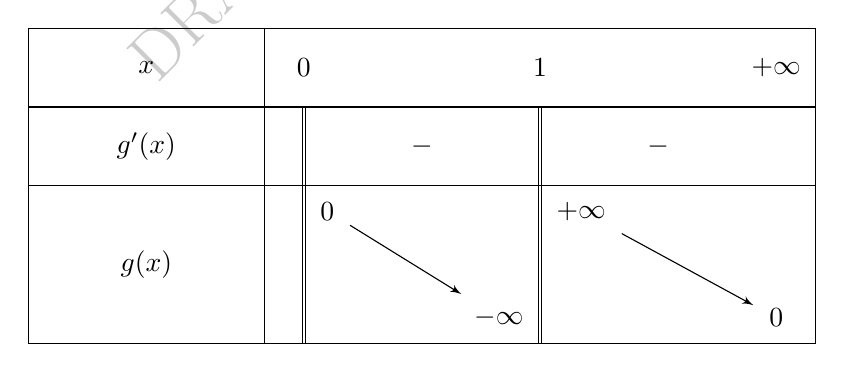
\begin{tikzpicture} 
\tkzTabInit[lgt=3, espcl=3]{$x$ /1, $g'(x)$ /1, $g(x)$ /2}{$0$, $1$, $+\infty$} 
\tkzTabLine{d, -, d, -,} 
\tkzTabVar{D+/$0$, -D+/ $-\infty$/$+\infty$ , -/$0$}
\end{tikzpicture} 
\end{center}


\underline{Graphe}

\quad

2) On considère l'ensemble $D = ]0,1/2[\cup]1,+\infty[$.

On définit l'intégrale $J(x)$ par : 
$J(x) =\int_{x}^{2x}g(t)dt$

Montrons que $J(x)$ existe pour tout $x\in D$.

 L'intégrale n'existe que si 1 n'est pas dans l'intervalle $(x, 2x)$, soit $1 < x$ ou $1 > 2x$, 
donc $x <1/2$ ou$ x > 1$, ce qui correspond à $D$. 

Avec la notation introduite en Q1), $J(x) = G(2x)-G(x)$. 

3) Soit l'ensemble $D^+ = [0,1/2[\cup ]1,+\infty[ = D \cup \lbrace 0\rbrace$

On définit l'application $f : D^+\longrightarrow \mathbb{R}$ par : 

$\forall x \in D,f(x) = J(x)$

$f(0)=0$

Montrer que $f$ est dérivable sur $D$, et calculer sa dérivée $f^{\prime}$.

Étudier le signe de $f^{\prime}$ et en déduire le sens des variations de $f$ 

Sur $D, J(x)= G(2x)-G(x)$, et donc, puisque $G'= g$, on a :$f'(x)$ existe et vaut : 
\[
f'(x) = 2g(2x)-g(x) = ln(x/2) /[(Lnx)(Ln2x)]\]

$\longrightarrow$ Pour pour $x < 1/2$, $f'(x)$ est $<0$, donc $f$ est décroissante. 

$\longrightarrow$ Pour $x > 1$, $f'(x)$ est $> 0$ si $x /2 > 1$, donc $x > 2$ ; de même, $f'(x) < 0$ si $x < 2$, et on a 
$f'(x) = 0$ si $x = 2$. 

On remarque aussi que la limite de $f'$ quand $x$ tend vers 0 est égale à 0. 
 
4) D'après les accroissements finis appliqués à $f$, $f = (2x-x)g(c), x \leqslant c \leqslant 2x$. 

Comme la fonction $g$ est décroissante (question 1), $g(x)\geqslant g(c)\geqslant g(2x)$, donc : 

\[x/\ln(2x)\leqslant f(x)\leqslant x/\ln x\]

et 

\[1/\ln(2x)\leqslant f(x)\leqslant 1/\ln x\]
 
On en déduit quand $x$ tend vers 0 : 

a) $f(x)$ tend vers 0 

b) $f(x) / x$ tend vers 0 

Donc on peut prolonger $f$ par continuité en 0. 

De même, la limite de $(f(x)-f (0))/(x-0) =f(x) /x$ est égale à 0, qui est aussi la limite 
de $f'$ en 0 (remarque de la question 3), donc $f$ est dérivable en 0. 

5) Toujours en utilisant la double inégalité de la question 4, on a : 
Quand $x$ tend vers $+\infty$ : 

a) $f(x)$ tend vers $+\infty$ 

b) $f(x) / x$ tend vers 0 

6) En étudiant brièvement $h(u)$ sur $]0, 1]$, on voit que $h$ est croissante de $-\infty$ à $1-ln2$ lorsque u passe de 0 à 1/2, admet un maximum égal à $1-ln2$ en 1/2 et décroit ensuite jusqu'à 0. 

Donc il existe un nombre $\alpha$, compris entre 0 et 1/2, tel que $h(\alpha) = 0$. 

Pour $u\geqslant\alpha$, $h(u)$ est positive ou nulle, donc $ln(u)\geqslant 2u-2$. 

Donc $1/ln(u)\leqslant 1/(2u-2)$. 

En reportant cette inégalité dans la définition de $f$, on voit que $f(x)$ est majorée par l'intégrale : 

\[
f(x)\leqslant \int_{x}^{2x}\frac{du}{2u-2}=\frac{1}{2}.\ln(\frac{2x-1}{x-1})\]
 
 Quand $x\rightarrow 1/2,\frac{1}{2}.\ln\left(\frac{2x-1}{x-1}\right)$ tend vers  $-\infty$ et donc $f$ aussi. 

7) Montrer que, $\forall u\geqslant 1, \ln(u)\leqslant u-1$. 
Déduisons la limite de $f$ quand  $x\rightarrow 1$. 

Comme en Question 6, en étudiant les variations de $v(u) = \ln(u)-(u-1)$, on trouve facilement que $\ln(u)\leqslant u-1$ quand $u\geqslant 1$. 

On en déduit en minorant $g(x)$ par $1/(u-1)$ dans l'intégrale que
 $f(x)\geqslant \ln(\frac{2x-1}{x-1})$; or $\ln(\frac{2x-1}{x-1})$ tend vers $+\infty$ quand $x\rightarrow 1$, donc f aussi. 

8) Construisons le tableau de variations de $f$ .   

Donc, il résulte de tout ce qui précède, que : 

Pour $x$ entre 0 et 1/2 : $f$ décroît de 0 à $-\infty$
 
Et pour $x\geqslant 1$ : 

a) de 1 à 2, $f$ décroît de $+\infty$ au minimum $m = J(2) = G(4)-G(2)$,  

b) puis $f$ croît de $m$ à $+\infty$ pour $x\geqslant 2$.

\underline{ Tableau de Variations}
\begin{center}
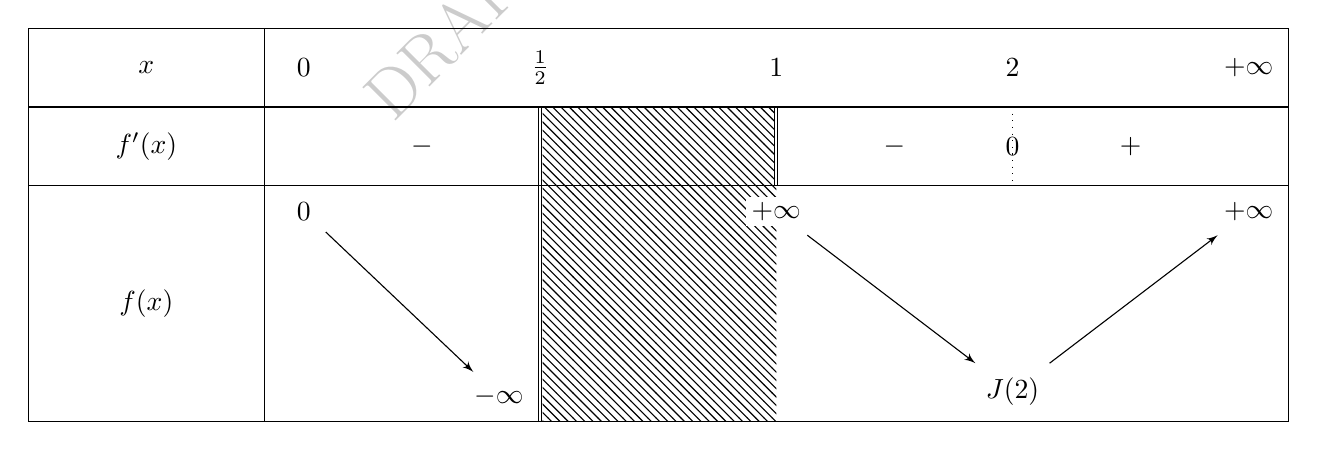
\begin{tikzpicture} 
\tkzTabInit[lgt=3, espcl=3]{$x$ /1, $f'(x)$ /1, $f(x)$ /3}{$0$, $\frac{1}{2}$, $1$, $2$,  $+\infty$} 
\tkzTabLine{, -,d, h, d, -,z ,+,} 
\tkzTabVar{+/$0$, -DH/ $-\infty$, +/$+\infty$ , -/$J(2)$, +/$+\infty$}
\end{tikzpicture} 
\end{center}







\medskip\textbf{Exercice 3}

1) Comparons les intégrales $A$ et $B$ :

$A=\int_{0}^{\frac{\pi}{4}}Ln(\cos x)dx$

$B= \int_{0}^{\frac{\pi}{4}}Ln(\cos(\frac{\pi}{4}- x))dx$.

 En faisant dans $B$ le changement de variable $u =\frac{\pi}{4}- x$, on obtient directement $A = B$.

2. Calculons l'intégrale $I=\int_{0}^{\frac{\pi}{4}}Ln(1+\tan x)dx$.

 On sait que :
 
\[\cos(\frac{\pi}{4}-x)=\frac{\cos x+\sin x}{\sqrt{2}}\]

\[
1+\tan x=\frac{\cos x+\sin x}{\cos x}\]

\begin{align*}
\ln(1+\tan x)&=\ln(\cos x+\sin x)-\ln(\cos x)\\
&=\ln(\sqrt{2})\cos(\frac{\pi}{4}-x)-\ln(\cos x)\\
&=\ln(\sqrt{2})+\ln(\cos(\frac{\pi}{4})-x)-\ln(\cos x)
\end{align*}


D'où, en passant à l'intégrale et comme $A = B$, on a 
\[I=\frac{\pi}{4}\ln(\sqrt{2})\]
 


\medskip\textbf{Sujet 14}

\textbf{Exercice 1}

1.a) Étudions, dans le même tableau de variations, les variations de $x(t)$ et $y(t)$ en fonction de $t$. 

$x'(t) = t + 1$
 
$y’(t) = 1-t $

Pour $t\in \mathbb{R}$, $x(t)$ décroit de $+\infty$ à -1/2, lorsque $t$ va de $-\infty
$ à -1, puis croît jusqu'à $+\infty$ pour $t$ allant de -1 à $+\infty$ ; $x(t)$ s'annule en $t = 0$. 

En outre, $x(1) = 3/2$.

\medskip 
$y(t)$ croît de $-\infty$ à 1/2, lorsque $t$ va de $-\infty$ à +1, puis décroît jusqu'à $-\infty$ pour $t$ allant de 1 à $+\infty$ ; $y(t)$ s'annule en $t = 0$. 

En outre, $y(-1) = -3/2$. 

b) Étudions les points de la courbe $C$ en lesquels la tangente est parallèle à l'un des axes de 
coordonnées. 

Cela revient à résoudre $x’(t) = 0$ et $y’(t) = 0$.  

$x’(t) = 0$ pour $t = -1$ (le point associé est (-1/2, -3/2)). 
$y’(t) = 0$ pour $t = 1$ (le point associé est (3/2, 1/2)). 

c) Précisons les points d'intersection de $C$ avec les axes $Ox$ et $Oy$. Donnons un vecteur 
directeur des tangentes en ces points. 

Avec l'axe des ordonnées : $x(t) = 0$ pour $t = 0$ et -2 

Pour $t = 0$, le point est $O (0, 0) $

Pour $t = -2$, le point correspondant est $A(0, -4)$  

Avec l'axe des abscisses : $y(t) = 0$ pour $t = 0$ et 2 

Pour $t = 0$, le point est $O (0, 0)$ 

Pour $t = 2$, le point correspondant est $B(4, 0)$  

La courbe $C$ coupe donc les axes en trois points : $O, A$ et $B$. 

Vecteur directeur des tangentes en $O, A$ et $B$ :
 
En $O, x’ = 1$ et $y’ = 1$ ; en $A, x’ = -1$ et $y’ = 3$ ; en $B, x’ = 3$ et $y’ = -1$. 

d) Donnons graphiquement l'allure de la courbe $C$, en positionnant les points remarquables déterminés. 

\textbf{Tableau de variation}


\begin{center}
    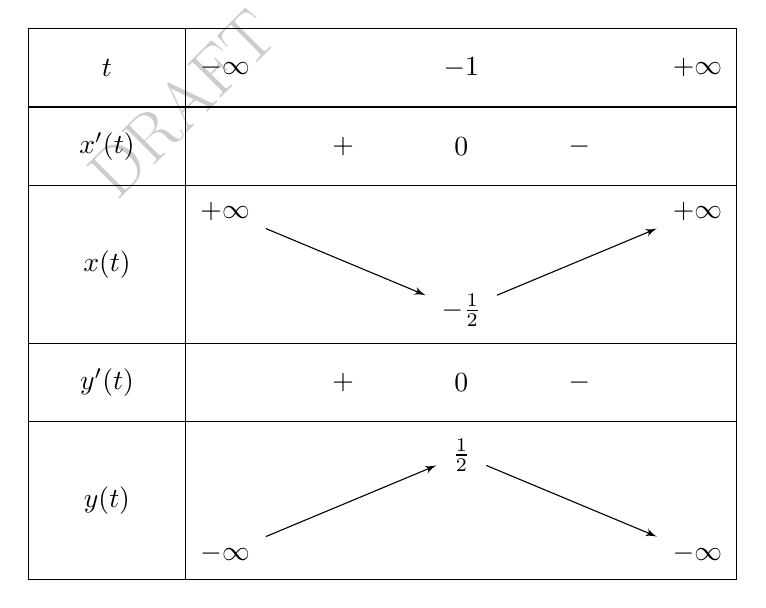
\begin{tikzpicture}
        \tkzTabInit[lgt=2, espcl=3]
        {$t$ /1, $x'(t)$ /1, $x(t)$ /2, $y'(t)$ /1, $y(t)$ /2}
        {$-\infty$, $-1$, $+\infty$}

        % Ligne des variations de x'(t)
        \tkzTabLine{, +, 0, -,}

        % Ligne des variations de x(t)
        \tkzTabVar{+/ $+\infty$, -/$-\frac{1}{2}$ ,  +/$+\infty$,}
        
        % Affichage du point (0,0) sur la flèche
       % \tkzTabIma{3}{2}{3}{$0$}

        
        % Ligne des variations de y'(t)
        \tkzTabLine{, +, 0, -,}

        % Ligne des variations de y(t)
        \tkzTabVar{-/ $-\infty$, +/$\frac{1}{2}$, -/$-\infty$}
    \end{tikzpicture}
\end{center}







\quad

\textbf{Allure de la courbe $C$}





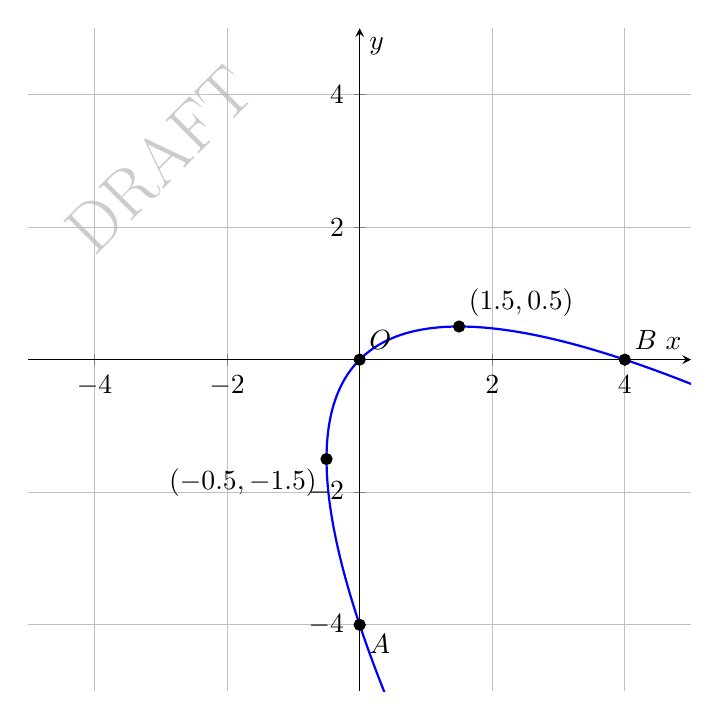
\begin{tikzpicture}
    \begin{axis}[
        axis lines = middle,
        xlabel = \( x \),
        ylabel = \( y \),
        xmin = -5, xmax = 5,
        ymin = -5, ymax = 5,
        grid = both,
        width = 10cm,
        height = 10cm,
        samples = 200,
        domain = -4:4,
        ]

        % Tracer la courbe C en utilisant des équations paramétriques
        \addplot [
            blue,
            thick,
            variable = \t, % Définir la variable de paramétrisation
            parametric, % Activer le mode paramétrique
        ] ({t + (t^2)/2}, {t - (t^2)/2});

        % Points remarquables
        \addplot [only marks, mark=*, mark size=2pt] coordinates {
            (0, 0) % Point O
            (0, -4) % Point A
            (4, 0) % Point B
            (-0.5, -1.5) % Point où x'(t) = 0
            (1.5, 0.5) % Point où y'(t) = 0
        };

        % Étiquettes des points
        \node at (axis cs: 0, 0) [above right] {\( O \)};
        \node at (axis cs: 0, -4) [below right] {\( A \)};
        \node at (axis cs: 4, 0) [above right] {\( B \)};
        \node at (axis cs: -0.5, -1.5) [below left] {\((-0.5, -1.5)\)};
        \node at (axis cs: 1.5, 0.5) [above right] {\((1.5, 0.5)\)};

    \end{axis}
\end{tikzpicture}





e) Donnons l'équation cartésienne $v(x, y) = 0$ de la courbe $C$. 

On remarque que $t = (x + y)/2$ 

En reportant dans la définition de $x(t)$, on a : 

$x = (x + y)^2/8 + (x + y)/2$ 

En développant, on obtient : 

$v(x, y) = x^2+ y^2 + 2xy-4x + 4y = 0$ 

2 – On se propose de déterminer précisément ce qu'est la courbe $C$. 

a) Le plan étant assimilé au plan complexe, on considère l'application $h$ qui, à tout 
point $M$ d'affixe $z$ du plan, associe un point $M'$ d'affixe $Z$, définie par : 

\[
Z= \frac{1}{\sqrt{2}}(1+i)z\]

 Donnons de façon précise la nature de l'application $h$. 

On remarque que $Z = h(z) = e^{i\pi/4}z$
 
$H$ est donc une rotation de centre $O$ et d'angle $\pi/4$. 

b) Soit $M$ le point d'affixe $z(t) = x(t) + i y(t)$.
 
Déterminons les coordonnées $X(t)$ et $Y(t)$ de $M’$, image de $M$ par $h$. 
Donnons une équation cartésienne $\varphi(X, Y) = 0$ de la courbe $C’$ des points $M$’. 
  
Soit $z(t) = \rho e^{i\theta} = \rho cos\theta + i\rho sin\theta$, avec $x(t) =\rho cos\theta$ et $y(t) =\rho sin\theta$. 

$Z = h(z) = e^{i\pi/4}z = \rho e^{i(\theta+\pi/4)} z$.
 
D'où $X(t) = (x(t - y(t))/2^{1/2}$  et $Y(t) = (x(t) + y(t))/2^{1/2}$ 

On en déduit : $Y = 2^{1/2}t$ et $X = 2^{-1/2} t^2$.

D'où la relation $\varphi(X, Y) = 0 = 4.2^{1/2} X-Y^2$
 
La courbe $C’$ est une parabole d'axe $Ox$.
 
Le courbe $C’$ est l'image de $C$ par la rotation de centre $O$ et d'angle $\pi/4$. La courbe $C$ est 
donc l'image de $C’$ par la rotation de centre $O$ et d'angle $- \pi/4$. 

C'est donc encore une parabole, dont l'axe est la deuxième bissectrice.

\medskip\textbf{Exercice 2}

Donnons la probabilité, l'espérance mathématique et la variance de la variables aléatoires $X$ lorsque $X$ suit chacune des lois discrètes usuelles.

\textbf{$\rightarrow$ Loi discrète uniforme}

\[P(X=k)=\frac{1}{n} \hspace{1cm} E(X)=\frac{n+1}{2} \text{ et } V(X)=\frac{n^2-1}{12}\]

\medskip\textbf{$\rightarrow$ Loi de Bernoulli de paramètre $p$}

\[P(X=1)=p \text{ et } P(X=0)=1-p \hspace{1cm}  E(X)=p \textbf{ et } V(X)=p(1-p)\]

\medskip\textbf{$\rightarrow$ Loi binomiale de paramètres $n$ et $p$}

\[P(X=k)=C_n^kp^k(1-p)^{n-k} \hspace{1cm} E(X)=np \text{ et } V(X)=np(1-p)\]

\medskip\textbf{$\rightarrow$ Loi de Poisson de paramètre $\lambda$}

\[P(X=k)=e^{-\lambda}\frac{\lambda^k}{k!} \text{ ou } k\in \mathbb{N} \hspace{1cm} E(X)=V(X)=\lambda\]

\medskip\textbf{$\rightarrow$ Loi Hypergéométrique de paramètres $(N,n,p)$}

\[p(X=k)=\frac{C_{N_p}^kC_{N-N_p}^{n-k}}{C_N^n} \hspace{1cm} E(X)=np \text{ et } V(X)=np(1-p)\frac{N-n}{N-1}\]

\medskip\textbf{$\rightarrow$ Loi géométrique de paramètre p}

\[P(X=k)=p(1-p)^{k-1} \hspace{1cm} E(X)=\frac{1}{p} \text{ et } V(X)=\frac{q}{p^2}\]

\medskip\textbf{$\rightarrow$ Loi Pascal de paramètre $n$ et $p$}

C'est la loi du nombres d'essais nécessaires pour observer $n$ fois un évènement $A$ de probabilité $p$. L'expérience devant se terminer par $A$.

\[P(X=k)=pC_{k-1}^{n-1}p^{n-1}(1-p)^{(k-1)-(n-1)}=C_{k-1}^{n-1}p^n(1-p)^{k-n} \text{ pour } k=n,n+1,\cdots,\infty\]

C'est la somme de $n$ loi géométriques indépendantes(apparition de $A$ pour la première fois, puis pour la deuxième fois, etc.).

\[E(X)=\frac{n}{p} \text{ et } V(X)=\frac{np}{p^2}\]

\medskip\textbf{$\rightarrow$ Loi binomiale négative}

C'est la loi du nombre d'échec nécessaires pour obtenir $n$ succès.

\[P(X=k)=C_{n+k-1}^{n-1}P^n(1-P)^k\]

C'est la loi de $X'=X-n$ ou $X$ suit la loi binomiale.

\[E(X)=nP \text{ et } V(X)=nP(1-P)\]


\medskip\textbf{Exercice 3}

1. La somme exacte que M.Barro touchera le $3^e$ mois correspond à $U_3$.

$U_3=U_2 +0.03U_2=(1+0.03)U_2=1.03*618 000 =\textbf{636 540}$

2. La nature de $(U_n)$

On a $\forall n\in N^*,U_{n+1}=U_n+0.03U_n=1.03U_n$.  Ainsi, $(U_n)$ est une suite géométrique de raison 1,03 et de premier terme 600 000.

Donc l'expression de $U_n$ en fonction de $n$ est donnée par $U_n=600 000(1.03)^n$.

3. La somme que M.Barro touchera le dernier mois$(12^e)$ est:

$U_{12}=600 000*1.03^{12}= \textbf{855456.5321}$

4. Déterminons la somme $S$

$S=U_1+U_2+...+U_{12}$

\hspace{0.358cm}$=U_1+1.03U_1+1.03^2U_1...+1.03^{12}U_1$.

\hspace{0.358cm}$=(1+1.03+1.03^2+...+1.03^{12})U_1$

\hspace{0.358cm}$=U_1\sum_{k=0}^{12}(1.03)^k$

\hspace{0.358cm}$=U_1\frac{1-1.03^{13}}{1-1.03}$. Il s'agit de l'application de la formule générale de la somme des $n$ premiers termes d'une suite géométrique de raison q et de premier terme $U_p$ donnée par $S_n=U_p\frac{1-q^{n-p+1}}{1-q}$

\hspace{0.358cm}$=600 000*15.6178$

\hspace{0.058cm}$\underline{S=9370674.269}$


\medskip\textbf{Sujet 15}

\medskip\textbf{Exercice 1}

1. Forme quadratique $q(x, y, z)$ et matrice associée $A$

La forme quadratique est donnée par :
\[
q(x, y, z) = x(x - 4y + 4z) + 2yz.
\]

\noindent En développant cette expression, nous obtenons :
\[
q(x, y, z) = x^2 - 4xy + 4xz + 2yz=x^2-2xy-2yx+2xz+2zx+yz+zy.
\]

\noindent La matrice symétrique associée $A$ est définie à partir des coefficients quadratiques, mixtes et linéaires :
\[
A = 
\begin{pmatrix}
1 & -2 & 2 \\
-2 & 0 & 1 \\
2 & 1 & 0
\end{pmatrix}.
\]

\noindent (a) Déterminons la signature de $q$ par deux méthodes

\textbf{Méthode 1 : Par élimination de Gauss} \\
On applique l'élimination de Gauss pour diagonaliser $A$ :

\begin{align*}
\begin{pmatrix}
\boxed{1} & -2 & 2 \\
-2 & 0 & 1 \\
2 & 1 & 0
\end{pmatrix}\begin{array}{c}
L_2\longleftarrow L_2+2L_1\\
L_3\longleftarrow L_3-2L_1
\end{array}
\to
\begin{pmatrix}
\boxed{1} & -2 & 2 \\
0 & -4 & 5 \\
0 & 5 & -4
\end{pmatrix}L_3\longleftarrow 4L_3+5L_2\\
\begin{pmatrix}
\boxed{1} & -2 & 2 \\
0 & -4 & 1 \\
0 & 0 & 9
\end{pmatrix}\begin{array}{c}
C_2\longleftarrow C_2+2C_1\\
C_3\longleftarrow C_3+C_2
\end{array}
\begin{pmatrix}
\boxed{1} & 0 & 0 \\
0 & -4 & -3 \\
0 & 0 & 9
\end{pmatrix}C_3\longleftarrow 4C_3-3C_2\\
\begin{pmatrix}
\boxed{1} & 0 & 0 \\
0 & -4 & 0 \\
0 & 0 & 36
\end{pmatrix}
\end{align*}
Donc $A\to \begin{pmatrix}
1 & 0 & 0 \\
0 & -4 & 0 \\
0 & 0 & 36
\end{pmatrix}$

La diagonalisation montre que $q$ a deux valeurs propres positives ($1$, $36$) et une valeur propre négative ($-4$). La signature de $q$ est donc $(2, 1, 0)$ ou 2 est le nombre de valeurs propres positive, 1 le nombre de valeurs propres négatives et 0 le nombre de valeurs propres nulles.

\textbf{Méthode 2 : Par les mineurs principaux emboîtés} \\
Les mineurs principaux de $A$ sont :
\begin{align*}
&\text{Premier mineur principal( en haux à gauche d'ordre 1)} M_1 = 1>0,\\ \quad 
&\text{Deuxième mineur principal( en haux à gauche d'ordre 2)}M_2 = 
\begin{vmatrix}
1 & -2 \\
-2 & 0
\end{vmatrix} = 4>0,\\ \quad 
&\text{Troisième mineur principal(A)}\det(A) = -9<0.
\end{align*}

Les signes des mineurs alternent, ce qui confirme une signature $(2, 1, 0)$.

(b) Factorisation $QR$ de $A$

La décomposition $QR$ consiste à écrire $A = QR$, où $Q$ est orthogonale et $R$ est triangulaire supérieure. Nous allons appliquer le processus de Gram-Schmidt à $A$, 

Les colonnes de $A$sont données par :\\
\[
a_1=\begin{pmatrix}
1\\
-2\\
2
\end{pmatrix}, \quad a_2=\begin{pmatrix}
-2\\
0\\
1
\end{pmatrix}, \quad a_3=\begin{pmatrix}
2\\
1\\
0
\end{pmatrix}
\]

\textbf{Étape 1 : Normalisation de $a_1$}

$\vert\vert a_1\vert\vert=\sqrt{1^2+(-2)^2+2^2}=\sqrt{9}=3$

Le premier vecteur orthonormal est :

\[q_1=\frac{a_1}{\vert\vert a_1\vert\vert}=\frac{1}{3}\begin{pmatrix}
1\\
-2\\
2
\end{pmatrix}=\begin{pmatrix}
\frac{1}{3}\\
-\frac{2}{3}\\
\frac{2}{3}
\end{pmatrix}\]

\medskip
\textbf{Étape 2 : Orthogonalisation de $a_2$ par rapport à $q_1$}

On calcule la projection de $a_2$ sur $q_1$ :

$proj_{q_1}(a_2)=(a_2^{\intercal}q_1)q_1$, ou $a_2^{\intercal}q_1=(-2, 0,1).\frac{1}{3}\begin{pmatrix}
1\\
-2\\
2
\end{pmatrix}=\frac{1}{3}((-2).1+0.(-2)+1.2)=0$

Ainsi $a_2$ est déjà orthogonal à $q_1$. Normalisons $a_2$ :

$\parallel a_2\parallel =\sqrt{(-2)^2+0^2+1^2}=\sqrt{5}$

Le deuxième vecteur orthonormal est :
\[q_2=\frac{a_2}{\vert\vert a_2\vert\vert}=\frac{1}{\sqrt{5}}\begin{pmatrix}
-2\\
0\\
1
\end{pmatrix}=\begin{pmatrix}
-\frac{2}{\sqrt{5}}\\
0\\
\frac{1}{\sqrt{5}}
\end{pmatrix}\]

\medskip
\textbf{Étape 3 : Orthogonalisation de $a_3$}

Calculons la projection de $a_3$ d'abord sur $q_1$ :

$proj_{q_1}(a_3)=(a_3^{\intercal}q_1)q_1$, ou $a_3^{\intercal}q_1=(2, 1,0).\frac{1}{3}\begin{pmatrix}
1\\
-2\\
2
\end{pmatrix}=\frac{1}{3}(2.1+1.(-2)+0.2)=0$

Ainsi $a_3$ est orthogonal à $q_1$.

\medskip
Calculons la projection de $a_3$  sur $q_2$ 

$proj_{q_2}(a_3)=(a_3^{\intercal}q_2)q_2$, ou $a_3^{\intercal}q_2=(2, 1,0).\frac{1}{\sqrt{5}}\begin{pmatrix}
-2\\
0\\
1
\end{pmatrix}=\frac{1}{\sqrt{5}}(2.(-2)+1.0+0.1)=\frac{-4}{\sqrt{5}}\neq 0$ alors $a_3$ n'est pas orthogonal à $q_2$.

Nous allons soustraire cette projection de $a_3$ pour la rendre orthogonale à $q_2$.

\[b_3=a_3-\langle a_3,q_2\rangle q_2=\begin{pmatrix}
2\\
1\\
0
\end{pmatrix}-\left(\frac{-4}{\sqrt{5}}\right)\begin{pmatrix}
\frac{-2}{\sqrt{5}}\\
0\\
\frac{1}{\sqrt{5}}
\end{pmatrix}=\begin{pmatrix}
2\\
1\\
0
\end{pmatrix}+\frac{4}{5}\begin{pmatrix}
2\\
0\\
-1
\end{pmatrix}=\begin{pmatrix}
2+\frac{8}{5}\\
1+0\\
0-\frac{4}{5}
\end{pmatrix}=\begin{pmatrix}
\frac{18}{5}\\
1\\
-\frac{4}{5}
\end{pmatrix}\]

La norme est $\parallel b_3\parallel =\sqrt{\left(\frac{18}{5}\right)^2+1^2+\left(-\frac{4}{5}\right)^2}=\frac{\sqrt{365}}{5}$

La troisième colonne orthonormée est $q_3=\frac{b_3}{\parallel b_3\parallel}=\frac{5}{\sqrt{365}}\begin{pmatrix}
\frac{18}{5}\\
1\\
-\frac{4}{5}
\end{pmatrix}=\begin{pmatrix}
\frac{18}{\sqrt{365}}\\
\frac{5}{\sqrt{365}}\\
-\frac{4}{\sqrt{365}}
\end{pmatrix}$

Ainsi la matrice orthogonale est : \[Q=\begin{pmatrix}
\frac{1}{3} & -\frac{2}{\sqrt{5}}& \frac{18}{\sqrt{365}} \\ 
-\frac{2}{3}& 0                 &  \frac{5}{\sqrt{365}} \\ 
\frac{2}{3} & \frac{1}{\sqrt{5}} & -\frac{4}{\sqrt{365}}
\end{pmatrix} \]

\quad

Calculons de $R$

La matrice $R$ est une matrice triangulaire supérieure qui contient les coefficients $r_{ij}$ obtenus en projetant  les colonnes de $A$ sur les vecteurs $q_1,q_2,q_3$.

Calcul des coefficient $r_{ij}$.

$r_{11}=\parallel a_1\parallel=03$ \quad   $r_{12}=\langle a_2,q_1\rangle=0$ (calculé précédemment).


$r_{13}=\langle a_3,q_1\rangle =0$, \quad $r_{22}\parallel a_2\parallel=\sqrt{5}$, \quad $r_{23}=\langle a_3,q_2\rangle=-\frac{4}{\sqrt{5}}$

$r_{33}=\parallel b_3\parallel=\frac{\sqrt{365}}{5}$

La matrice triangulaire supérieure $R$ est \[R=\begin{pmatrix}
3 & 0 & 0 \\ 
0 & \sqrt{5} & -\frac{4}{\sqrt{5}} \\ 
0 & 0 & \frac{\sqrt{365}}{5}
\end{pmatrix} \]




2. Étude des séries

(a) Convergence des séries

\textbf{Première série : $\sum \frac{(n+2)^n}{n^{n+2}}$} \\

Soit $a_n=\frac{(n+2)^n}{n^{n+2}}\Longrightarrow a_{n+1}=\frac{(n+3)^{n+1}}{{n+1}^{n+3}}$

En appliquant le critère de d'Alembert :
\[
\lim_{n \to +\infty} \frac{a_{n+1}}{a_n} = \lim_{n \to +\infty} \frac{(n+3)^{n+1} n^{n+2}}{(n+2)^{n+1} (n+1)^{n+3}}\approx \lim_{n \to +\infty} \frac{(n)^{n+1} n^{n+2}}{(n)^{n+1} (n)^{n+3}}\approx \lim_{n \to +\infty} \frac{1}{n}=0<1.
\]
Après simplifications, ce critère donne une limite 0 inférieure à $1$, donc la série converge.

\textbf{Deuxième série : $\sum \frac{\sqrt{5n+1}}{n!}$} \\

Posons $a_n=\frac{\sqrt{5n+1}}{n!}\Rightarrow a_{n+1}=\frac{\sqrt{5n+6}}{{n+1}!}$

En appliquant le critère de d'Alembert :

\[
\lim_{n \to +\infty} \frac{a_{n+1}}{a_n} = \lim_{n \to +\infty} \frac{\frac{\sqrt{5n+6}}{{n+1}!}}{\frac{\sqrt{5n+1}}{n!}}=\lim_{n \to +\infty}\frac{\sqrt{5n+6}n!}{(n+1)n!\sqrt{5n+1}}\approx\lim_{n \to +\infty}\frac{\sqrt{5n}}{(n+1)\sqrt{5n}}=0<1\], alors la série converge d'après le critère de d'Alembert

(b) Rayon de convergence de la série entière

Pour la série entière $\sum \frac{3^n(n+7)^3x^n}{n+3}$, on utilise le critère du rayon de convergence :

\begin{align*}
R &= \frac{1}{\limsup_{n \to \infty} \sqrt[n]{\left|\frac{3^n(n+7)^3}{n+3}\right|}}\\
&\approx\frac{1}{\limsup_{n \to \infty} \sqrt[n]{\left|\frac{3^nn^3}{n}\right|}}\\
&\approx\frac{1}{\limsup_{n \to \infty} \sqrt[n]{\left|3^nn^2\right|}}=\frac{1}{\limsup_{n \to \infty} 3n^{\frac{2}{n}}}=\frac{1}{\limsup_{n \to \infty} 3e^{\frac{2\ln(n)}{n}}}=\frac{1}{3}
\end{align*}
On trouve $R = \frac{1}{3}$.

3. Fonction homogène $f(x, y)$

La fonction est donnée par :
\[
f(x, y) = \frac{2\sqrt{x} + 3\sqrt{y}}{3x^2 + xy + 2y^2}.
\]

(a) Homogénéité positive et degré

Pour prouver que $f(x, y)$ est homogène, on calcule $f(\lambda x, \lambda y)$ :
\[
f(\lambda x, \lambda y) = \frac{2\sqrt{\lambda x} + 3\sqrt{\lambda y}}{3(\lambda x)^2 + (\lambda x)(\lambda y) + 2(\lambda y)^2}.
\]
Après simplifications, on trouve que $f(\lambda x, \lambda y) = \lambda^{-\frac{3}{2}} f(x, y)$, donc $f(x, y)$ est homogène de degré $-\frac{3}{2}$.

(b) Degré d'homogénéité de $(\frac{\partial^2 f}{\partial x \partial y})^3$

Si $f$ est homogène de degré $\alpha$, alors chaque dérivée partielle suit la relation :

\[
\frac{\partial f}{\partial x } \text{ est homogène de degré } \alpha - 1.\\
\frac{\partial^2 f}{\partial x \partial y} \text{ est homogène de degré } \alpha - 2.
\]
Ici, $\alpha = -\frac{3}{2}$, donc $\frac{\partial^2 f}{\partial x \partial y}$ est homogène de degré $-\frac{3}{2}-2=-\frac{7}{2}$. Ainsi $(\frac{\partial^2 f}{\partial x \partial y})^3$ est homogène de degré $(-\frac{7}{2})\times 3$.

(c) Calcul de l'expression

Nous calculons :
\[
x^2 \frac{\partial^2 f}{\partial x^2} + 2xy \frac{\partial^2 f}{\partial x \partial y} + y^2 \frac{\partial^2 f}{\partial y^2}.
\]

Utilisons une propriété fondamentale des fonctions homogènes (Formule d'Euler): si $f$ est homogène de degré $\alpha$, alors :


\[\sum_{k=1}^{n}x_k \frac{\partial f}{\partial x_k}(x)=\alpha f(x,y)\]


Dans notre cas :

\[
x^2 \frac{\partial^2 f}{\partial x^2} + 2xy \frac{\partial^2 f}{\partial x \partial y} + y^2 \frac{\partial^2 f}{\partial y^2}=\alpha(\alpha-1)f(x,y).
\]

Ainsi : 

\[
x^2 \frac{\partial^2 f}{\partial x^2} + 2xy \frac{\partial^2 f}{\partial x \partial y} + y^2 \frac{\partial^2 f}{\partial y^2}=-\frac{3}{2}(-\frac{3}{2}-1)f(x,y)=\frac{15}{4}\frac{2\sqrt{x} + 3\sqrt{y}}{3x^2 + xy + 2y^2}.
\]






\medskip
\textbf{Exercice 2}

$X$ est une variable aléatoire prenant des valeurs dans $\{0,1,2,3,4\}$, représentant le nombre de retards subis sur 4 appels.

1(a) Déterminons la loi de 
$X$, son espérance et sa variance

\textbf{Loi de $X$ :}

$X$ suit une loi binomiale de paramètres $(n;p)=(4;0,25)$ avec $n=4$(nombre d'appels) et $p=0,25$ (probabilité de retard).

La probabilité que $X=k$ (exactement $k$ retards sur 4 appels) est donnée par :

$P(X=k)=C_4^k(0,25)^k(0,75)^{4-k}$, 

Donc les probabilités sont :

$P(X=0)=C_4^0(0,25)^0(0,75)^{4-0}=0,3164$       $P(X=1)=C_4^1(0,25)^1(0,75)^{4-1}=0,4218$

$P(X=2)=C_4^2(0,25)^2(0,75)^{4-2}=0,2109$
   $P(X=3)=C_4^3(0,25)^3(0,75)^{4-3}=0,0468$

$P(X=4)=C_4^4(0,25)^4(0,75)^{4-4}0,0039$

\medskip
\textbf{Espérance $E(X)$}

$X$ suit la loi binomiale de paramètre $n=4$ et $p=0,25$ alors l'espérance est donnée par :

$E(X)=n.p=4\times 0,25=1$

\medskip
\textbf{Variance $V(X)$}

La variance est donnée par :

$V(X)=n.p(1-p)=4\times 0,25\times (1-0,25)=0,75$

(b) Calculons la probabilité de l'évènement : "Le client a au moins subi un retard".

Cela revient à calculer $P(X\geq 1)$

$P(X\geq 1)=1-P(x=0)=1-0,3164=0,6836$

(2) (a) Exprimons la probabilité conditionnelle de $Z = k$ sachant que $Y = n$.

Conditionnellement au fait que $Y=n$, il y a exactement $n$ appels dans la journée.

parmi ces $n$ appels, $Z$ suit une loi binomiale $B(n,p)$ avec $p=0,25$

Donc :

$P(Z=k/Y=n)=C_n^k(0,25)^k(0,75)^{n-k}$

 
 \medskip
 (b) Déduisons la probabilité de $"Z = k$ et $Y = n"$.
 
$P(Z=k,Y=n)=P(Z=k/Y=n)P(Y=n)$ avec,

 $P(Z=k/Y=n)=C_n^kp^k(1-p)^{n-k}$ et $P(Y=n)=e^{-m}\frac{m^n}{n!}$ car $Y$ suit une loi poisson de paramètre $m$

Donc,
\begin{align*}
P(Z=k,Y=n)&=C_n^kp^k(1-p)^{n-k}\times e^{-m}\frac{m^n}{n!} \text{ avec }   C_n^k=\frac{n!}{k!(n-k)!}, \text{ alors, } \\
P(Z=k,Y=n)&=\frac{n!}{k!(n-k)!}\times p^k(1-p)^{n-k}\times e^{-m}\frac{m^n}{n!}=\frac{p^k(1-p)^{n-k}m^n}{k!(n-k)!}.e^{-m}
\end{align*}
 
 
(c) Déterminons la loi de$ Z$. On trouvera que $Z$ suit une loi de Poisson de paramètre
 $m\times 0,25$.
 
 Pour trouver la loi de $Z$, il suffit de sommer sur tous les $n$ possibles.
 
\begin{align*}
P(Z=k)&=\sum_{n=k}^{\infty}P(Z=k,Y=n)=\sum_{n=k}^{\infty}P(Z=k/Y=n)P(Y=n)\\
&=\sum_{n=k}^{\infty}\frac{p^k(1-p)^{n-k}m^n}{k!(n-k)!}.e^{-m}=\sum_{n=k}^{\infty}\frac{p^k(1-p)^{n-k}m^{n-k+k}}{k!(n-k)!}.e^{-m}\\
&=\sum_{n=k}^{\infty}\frac{p^k(1-p)^{n-k}m^{n-k}m^k}{k!(n-k)!}.e^{-m}=\sum_{n=k}^{\infty}\frac{(p.m)^k(m(1-p))^{n-k}}{k!(n-k)!}.e^{-m}\\
&=\frac{(p.m)^k}{k!}.e^{-m}\sum_{n=k}^{\infty}\frac{(m(1-p))^{n-k}}{(n-k)!}
\end{align*}

En posant $n-k=j$, on a :

\[P(Z=k)=\frac{(p.m)^k}{k!}.e^{-m}.\sum_{j=0}^{\infty}\frac{(m(1-p))^j}{j!}\]

La somme est une série exponentielle. En effet, le développement limité de la fonction $x\longmapsto e^x$ en 0 est :

\[\sum_{j=0}^{\infty}\frac{x^j}{j!}=e^x \text{ alors } \sum_{j=0}^{\infty}\frac{(m(1-p))^j}{j!}=e^{m(1-p)}\]

Donc,

\[P(Z=k)=\frac{(p.m)^k}{k!}.e^{-m}.e^{m(1-p)}=\frac{(p.m)^k}{k!}.e^{-m.p}\]

Elle correspond à la probabilité d'une loi poisson de paramètre $m.p$.

Donc $Z$ suit une loi poisson de paramètre $m.p$.

 
(3) La loi de $U$ 

Le problème ici suit un schéma de Bernoulli. Le premier appel en retard correspond au \textbf{ nombre d'appels avant le premier succès} dans une suite de Bernoulli avec pour probabilité $p=0,25$.

Puisque $U$ correspond au premier succès après un certain nombre d'échecs, alors la variable $U$ suit une \textbf{loi géométrique} de paramètre $p$, donnée par :

\[
P(U=k)=p.(1-p)^{k-1},\hspace{0.7cm} k\in \mathbb{N}\]

\medskip
\textbf{Exercice 3}

$f(x)=\int_{x}^{2x}\frac{du}{u+\sin u}$
 
 
 1.a) Justifions l'existence de $f$.
 
 
 \textbf{Continuité de $\frac{1}{u+\sin u}$ sur $[x,2x]$}
 
 La fonction $u+\sin u$ est continue, car $u$ est une fonction linéaire et $\sin u$ est continue.
 
 Le dénominateur $u+\sin u> 0$ pour $u>0$, car $u>0$ et $\sin u\in [-1,1]$. Donc $u+\sin u\neq 0$.
 
 Ainsi $\frac{1}{u+\sin u}$ est bien continue sur $[x,2x]$.
 
 \medskip
 \textbf{Bornitude de $\frac{1}{u+\sin u}$ sur $[x,2x]$}
 
 $u+\sin u>u-1$ pour $u>1$. Donc $\frac{1}{u+\sin u}\leq\frac{1}{u-1}$, ce qui prouve que $\frac{1}{u+\sin u}$ est bornée.
 
 Par conséquent, l'intégrale $f(x)=\int_{x}^{2x}\frac{du}{u+\sin u}$ est bien définie.
 
 
 
 b) Étudions la parité de $f$.
 
 $f(x)=\int_{x}^{2x}\frac{du}{u+\sin u}$
 
 $f(-x)=\int_{-x}^{-2x}\frac{du}{u+\sin u}$
 
 Posons :$v=-u$ donc $dv=-du$
 
 En changeant des bornes :
 
$ \cdot$ Quand $u=-x$, $v=x$
 
$ \cdot$ Quand $u=-2x$, $v=2x$
 
 L'intégrale devient :
 
 $f(-x)=\int_{x}^{2x}\frac{-dv}{-v+\sin(-v)}$
 
 Simplifions cette expression :
 
 $\sin(-v)=-\sin(v)$, alors $-v+\sin(-v)=-v-\sin v=-(v+\sin(v)$.
 
 Ainsi 

 $f(-x)=\int_{x}^{2x}\frac{-dv}{-(v+\sin(v))}\int_{x}^{2x}\frac{dv}{v+\sin(v)}=f(x)$ puisque la variable est muette.
 
 On a :$f(x)=f(-x)$ alors $f$ est paire.
 
 c) Montrons que $\forall x>0, \hspace{0.1cm}f(x)>0$
 
 La fonction intégrée $\frac{1}{u+\sin u}>0$ pour $u>0$
 
 L'intégrale d'une fonction positive sur un intervalle $[x,2x]$ est positive :
 
 Alors, $\forall x>0, f(x)=\int_{x}^{2x}\frac{du}{u+\sin u}>0$
 
 Dans la suite on supposera que $x>0$
 
 2. Calculons $f'(x)$, 
 
 D'après la formule de Leibniz pour les intégrales à bornes variables, on a :
\[
f'(x) = \frac{\partial}{\partial x} \int_x^{2x} \frac{1}{u + \sin u} \, du = \frac{1}{2x + \sin(2x)} \cdot \frac{\partial}{\partial x}(2x) - \frac{1}{x + \sin x} \cdot \frac{\partial}{\partial x}(x).
\]

Les dérivées des bornes \( 2x \) et \( x \) donnent respectivement :
\[
\frac{\partial}{\partial x}(2x) = 2 \quad \text{et} \quad \frac{\partial}{\partial x}(x) = 1.
\]

Ainsi, \( f'(x) \) s'écrit :
\[
f'(x) = \frac{2}{2x + \sin(2x)} - \frac{1}{x + \sin x}.
\]

 Simplification de \( f'(x) \)

Mettons \( f'(x) \) sous une seule fraction. Le dénominateur commun est \((x + \sin x)(2x + \sin(2x))\), et \( f'(x) \) devient :
\[
f'(x) = \frac{2(x + \sin x) - (2x + \sin(2x))}{(x + \sin x)(2x + \sin(2x))}.
\]

Développons le numérateur :
\[
2(x + \sin x) = 2x + 2\sin x, \quad -(2x + \sin(2x)) = -2x - \sin(2x).
\]

Ainsi, le numérateur est donné par :
\[
2x + 2\sin x - 2x - \sin(2x) = 2\sin x - \sin(2x).
\]

En utilisant la formule de double angle \( \sin(2x) = 2\sin x \cos x \), on peut réécrire :
\[
2\sin x - \sin(2x) = 2\sin x - 2\sin x \cos x = 2\sin x(1 - \cos x).
\]

Finalement, on obtient :
\[
f'(x) = \frac{2\sin x(1 - \cos x)}{(x + \sin x)(2x + \sin(2x))}.
\]

Étude du signe de \( f'(x) \)

- Numérateur :\( 2\sin x(1 - \cos x) \).

  - Pour \( x > 0 \), on a \( \sin x \geq 0 \) et \( 1 - \cos x \geq 0 \) (car \( \cos x \leq 1 \)).
  - Donc, \( 2\sin x(1 - \cos x) \geq 0 \).

- Dénominateur : \( (x + \sin x)(2x + \sin(2x)) \).

  - Pour \( x > 0 \), \( x + \sin x > 0 \) et \( 2x + \sin(2x) > 0 \), donc le dénominateur est strictement positif.

Conclusion : \( f'(x) \geq 0 \) pour \( x > 0 \).

 Variations de \( f(x) \)

Puisque \( f'(x) \geq 0 \) pour \( x > 0 \), la fonction \( f(x) \) est \textbf{croissante} sur \( ]0, +\infty[ \).

Conclusion

 La dérivée de \( f(x) \) est donnée par :
\[
f'(x) = \frac{2\sin x(1 - \cos x)}{(x + \sin x)(2x + \sin(2x))}.
\]

 Comme \( f'(x) \geq 0 \) pour \( x > 0 \), la fonction \( f(x) \) est strictement croissante sur \( ]0, +\infty[ \).

 
 

 
 3.(a) Trouvons pour $u>1$, un encadrement de $\frac{1}{u+\sin u}$ puis pour $x>1$ un encadrement de $f(x)$.
 
 On a :
 
 $\bullet$ Pour $u>1$
 
 \[-1\leq \sin u\leq 1\Rightarrow u-1\leq u+\sin u\leq u+1\Rightarrow \frac{1}{u+1}\leq \frac{1}{u+\sin u}\leq \frac{1}{u-1} \text{ pour } u> 1\] 
 
 \medskip
 $\bullet$ Pour $x>1$
 
 Appliquons l'intégrale à l'encadrement précédent :
 
 \[
 \int_{x}^{2x}\frac{1}{u+1}du\leq \int_{x}^{2x}\frac{1}{u+\sin u}du\leq \int_{x}^{2x}\frac{1}{u-1}du\]
 
 \[\int_{x}^{2x}\frac{1}{u+1}du=\ln(2x+1)-\ln(x+1) \text{ et } \int_{x}^{2x}\frac{1}{u-1}du=\ln(2x-1)-\ln(x-1)\]
 
 Donc :
 
 \[\ln\left(\frac{2x+1}{x+1}\right)\leq f(x)\leq \ln\left(\frac{2x-1}{x-1}\right)\]
 
(b) Déterminons \[
\lim_{x\to +\infty}f(x)
\]

\[\lim_{x\to +\infty}\ln\left(\frac{2x+1}{x+1}\right)\leq \lim_{x\to +\infty}f(x)\leq \lim_{x\to +\infty}\ln\left(\frac{2x-1}{x-1}\right)\]
\[\ln(2)\leq \lim_{x\to +\infty}f(x)\leq ln(2)\Rightarrow \lim_{x\to +\infty}f(x)=ln(2)\]

\medskip
\textbf{Exercice 4}

Calculons la limite des suites suivantes :

1. \[
u_n=n\sum_{k=0}^{n-1}\frac{1}{n^2+k^2}
\]

Pour étudier la limite, il est utile de transformer cette somme en une somme de Darboux(Riemann).

On remarque que $k\in \{0,1,2,...,n-1\}$,  et le terme général peut être réécrit en divisant le numérateur et le dénominateur par $n^2$ :

\[\frac{1}{n^2+k^2}=\frac{1}{n^2}.\frac{1}{1+(\frac{k}{n})^2}\]

Ainsi, $u_n$ devient :

\[u_n=\frac{1}{n}\sum_{k=0}^{n-1}\frac{1}{1+(\frac{k}{n})^2}\]. On reconnait une somme de type Riemann. En posant $x=\frac{k}{n}$, on obtient une approximation de l'intégrale définie:

\[\lim_{n\to +\infty} u_n=\int_0^1\frac{1}{1+x^2}dx=[\arctan(x)]_0^1=\arctan(1)-\arctan(0)=\frac{\pi}{4}\]


2. \[
v_n=\prod_{k=1}^{n}\left(1+\frac{k^2}{n^2}\right)^{\frac{1}{n}}.
\]

\textbf{Expression logarithmique :} Pour étudier cette suite, prenons le logarithme pour simplifier les produits:

\[\ln\left(\prod_{k=1}^{n}\left(1+\frac{k^2}{n^2}\right)^{\frac{1}{n}}\right)=\frac{1}{n}\sum_{k=1}^n\ln\left(1+\frac{k^2}{n^2}\right)\]

Ainsi 
\[
v_n=\prod_{k=1}^{n}\left(1+\frac{k^2}{n^2}\right)^{\frac{1}{n}}= e^{\frac{1}{n}\sum_{k=1}^n\ln\left(1+\frac{k^2}{n^2}\right)}.
\]

On sait qu'en $x=0$, $ \ln(1+x) \stackrel{ 0 }{\sim} x $

Si $n\to +\infty$, $\frac{k^2}{n^2}\to 0$ alors $\ln(1+\frac{k^2}{n^2})\sim \frac{k^2}{n^2}$


En reportant dans $v_n$ on obtient la somme simplifiée :

$\frac{1}{n}\sum_{k=1}^n\ln\left(1+\frac{k^2}{n^2}\right)\sim \frac{1}{n}\sum_{k=1}^n\frac{k^2}{n^2}$

\medskip
\textbf{Limite de la somme :}

\[\lim_{n\to +\infty} \frac{1}{n}\sum_{k=1}^n\frac{k^2}{n^2}=\lim_{n\to +\infty}\frac{1}{n^3}\sum_{k=1}^n k^2 \text{ avec } \sum_{k=1}^n k^2=\frac{n(n+1)(2n+1)}{6}\]

\[\lim_{n\to +\infty} \frac{1}{n}\sum_{k=1}^n\frac{k^2}{n^2}=\lim_{n\to +\infty}\frac{1}{n^3}.\frac{n(n+1)(2n+1)}{6}=\lim_{n\to +\infty}\frac{(n+1)(2n+1)}{6n^2}=\frac{2}{6}=\frac{1}{3}\]

\medskip
En revenant à l'expression de $v_n$ :

\[\lim_{n\to +\infty}v_n=e^{\frac{1}{3}}\]










\newpage


\section*{\textbf{E. CORRECTIONS D'ANCIENS SUJETS}}

\medskip\textbf{SESSION 2016}

\medskip\textbf{Exercice 1}

On donne la courbe paramétrée suivante $(C)$ définie par : 
\[
\begin{cases}
x(t)=\cos{3t}\\
y(t)=\sin{2t}
\end{cases}\forall {t\in \mathbb{R}}
\]
1. Montrons que la courbe peut être entièrement obtenue en l'étudiant sur $[0,\pi]$

Vérifions la parité de $x(t)$ et $y(t)$

On a :

\[             
\begin{cases}  
x(-t)=\cos{(-3t)}=\cos{3t}=x(t)\\
y(-t)=\sin{(-2t)}=-\sin{(2t)}=-y(t)
\end{cases}
\]

$x(t)$ est paire et $y(t)$ impaire. Ainsi la courbe $(C)$ est symétrique par rapport à l'axe des abscisses. D'où le domaine d'étude de $(C)$ peut être réduit à $[0,\pi]$.

2. Dressons le tableau commun de variation des fonctions $x$ et $y$

\medskip Étudions $x(t)$ et $y(t)$

\textbf{Étude de $x(t)$ sur $[0,\pi]$}

$x(t)=\cos{3t}\Rightarrow x'(t)=-3\sin 3t$

$x'(t)=0\Rightarrow -3\sin 3t=0\Rightarrow \sin 3t=0=\sin 0$

\[
\Rightarrow\begin{cases}
3t=0+2k\pi\\
3t=\pi-0+2k\pi
\end{cases}\Rightarrow \begin{cases}
t=\frac{2k\pi}{3}\\
ou\\
t=\frac{\pi}{3}+\frac{2k\pi}{3}
\end{cases}
\]

-Pour $k=0$, $t=0$ ou $t=\frac{\pi}{3} $

-Pour $k=1$, $t=\frac{2k\pi}{3}$ ou $t=\pi$

\textbf{Tableau de signe de $x'(t)$}

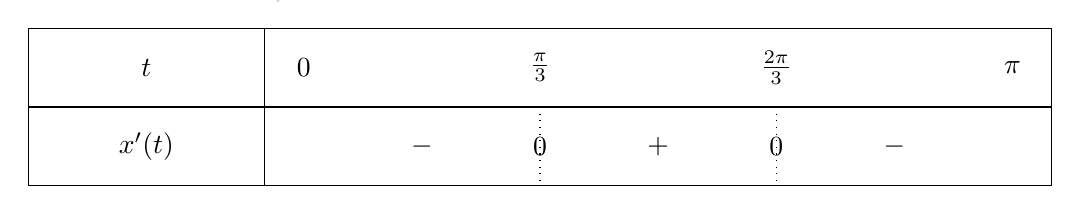
\begin{tikzpicture}
  \tkzTabInit[lgt=3, espcl=3]{$t$ /1, $x'(t)$ /1}{$0$, $\frac{\pi}{3}$, $\frac{2\pi}{3}$, $\pi$}
  \tkzTabLine{, -, z, +, z, -,}
\end{tikzpicture}

\underline{Variations de $x(t)$}

\[
\begin{cases}
\forall t\in [0,\frac{\pi}{3}],x'(t)\leq 0\hspace*{0.5cm} alors\hspace*{0.5cm} x(t)\hspace*{0.5cm} est \hspace*{0.5cm}decroissante\\
\forall t\in [\frac{\pi}{3}, \frac{2\pi}{3}], x'(t)\geq 0 \hspace*{0.5cm} alors\hspace*{0.5cm} x(t)\hspace*{0.5cm} est\hspace*{0.5cm} croissante\\
\forall t\in [\frac{2\pi}{3},\pi], x'(t)\leq 0\hspace*{0.5cm} alors\hspace*{0.5cm} x(t)\hspace*{0.5cm} est\hspace*{0.5cm} decroissante
\end{cases}
\]

\medskip\textbf{Étude de $y(t)$ sur $[0,\pi]$}

$y(t)=\sin{2t}\Rightarrow y'(t)=2\cos 2t$

$y'(t)=0\Rightarrow \cos 2t=0=\cos\frac{\pi}{2}$

\[
\begin{cases}
2t=\frac{\pi}{2}+2k\pi\\
2t=-\frac{\pi}{2}+2k\pi
\end{cases}\Rightarrow
\begin{cases}
t=\frac{\pi}{4}+k\pi\\
t=-\frac{\pi}{4}+k\pi
\end{cases}
\]

-Pour $k=0$, $t=\frac{\pi}{4}$

-Pour $k=1$, $t=\frac{3\pi}{4}$

Tableau de signe de $y'(t)$

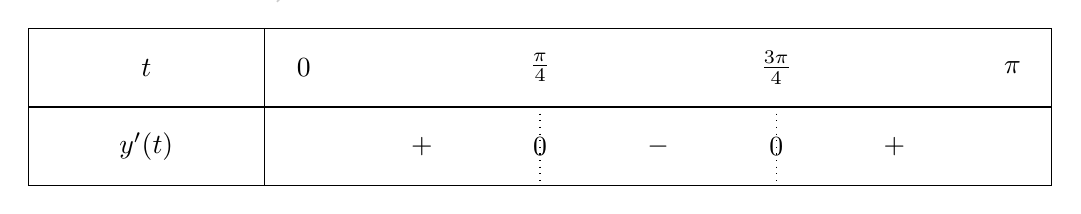
\begin{tikzpicture}
  \tkzTabInit[lgt=3, espcl=3]{$t$ /1, $y'(t)$ /1}{$0$, $\frac{\pi}{4}$, $\frac{3\pi}{4}$, $\pi$}
  \tkzTabLine{, +, z, -, z, +,}
\end{tikzpicture}

\underline{Variations de $y(t)$}

\[
\begin{cases}
\forall t\in [0,\frac{\pi}{4}],y'(t)\geq 0\hspace*{0.5cm} alors\hspace*{0.5cm} y(t)\hspace*{0.5cm} est \hspace*{0.5cm}croissante\\
\forall t\in [\frac{\pi}{4}, \frac{3\pi}{4}], y'(t)\leq 0 \hspace*{0.5cm} alors\hspace*{0.5cm} y(t)\hspace*{0.5cm} est\hspace*{0.5cm} decroissante\\
\forall t\in [\frac{3\pi}{4},\pi], y'(t)\leq 0\hspace*{0.5cm} alors\hspace*{0.5cm} y(t)\hspace*{0.5cm} est\hspace*{0.5cm} croissante
\end{cases}
\]

\medskip\textbf{Tableau commun de variation des fonctions $x$ et $y$}

$x(0)=1$, $x(\frac{\pi}{4})=-\frac{\sqrt{2}}{2}$, $x(\frac{\pi}{3})=-1$, $x(\frac{2\pi}{3})=1$, $x(\frac{3\pi}{4})=-1$, $x(\pi)=-1$

$x'(0)=0$, $x'(\pi)=0$

$y(0)=0$, $y(\frac{\pi}{4})=1$, $y(\frac{\pi}{3})=\frac{\sqrt{3}}{2}$, $y(\frac{2\pi}{3})=-\frac{\sqrt{3}}{2}$, $y(\frac{3\pi}{4})=-1$, $y(\pi)=0$

$y'(0)=2$, $y'(\pi)=2$

\begin{center}
\resizebox{\textwidth}{!}{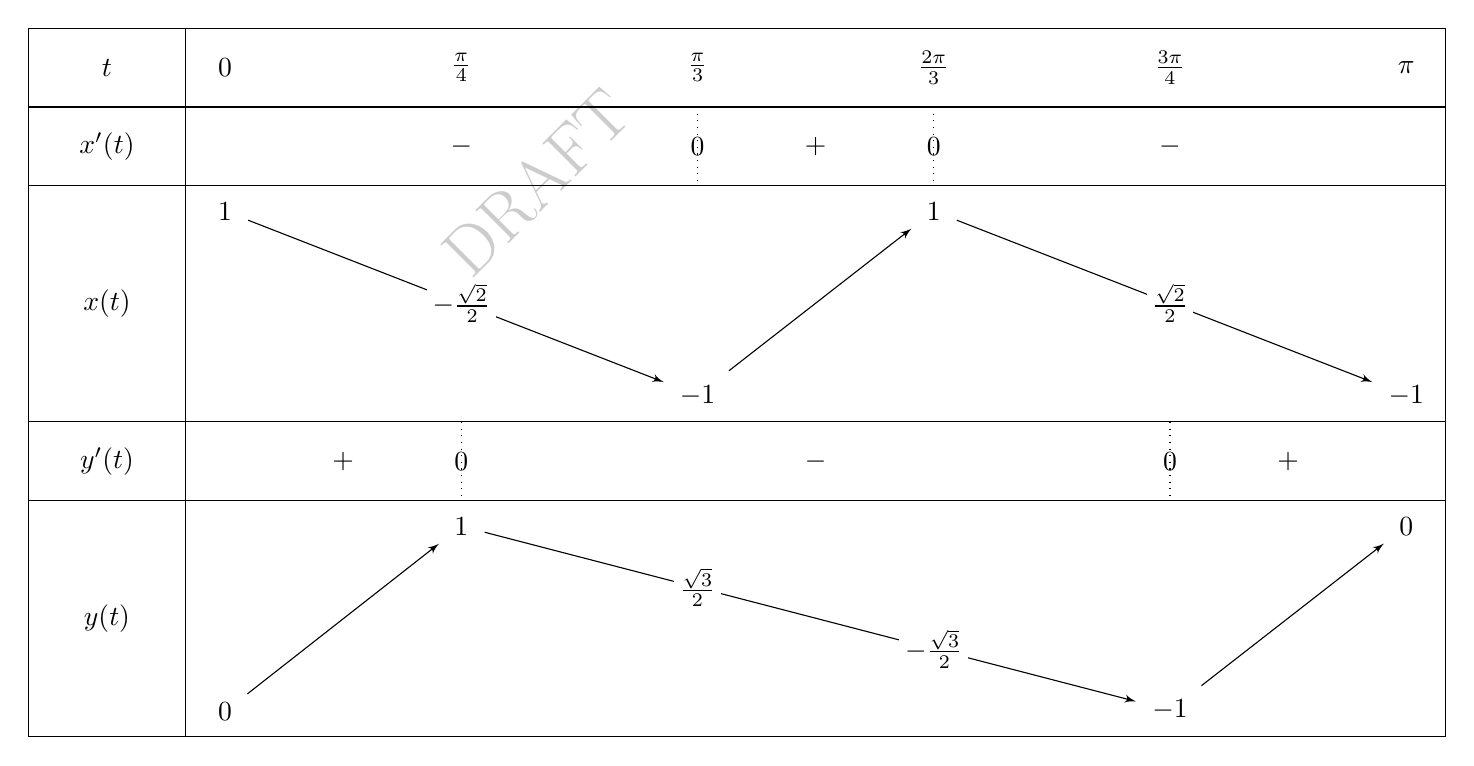
\begin{tikzpicture}
    % Initialisation du tableau
    \tkzTabInit[lgt=2, espcl=3]
    {$t$ /1, $x'(t)$ /1, $x(t)$ /3, $y'(t)$ /1, $y(t)$ /3} 
    {$0$, $\frac{\pi}{4}$, $\frac{\pi}{3}$, $\frac{2\pi}{3}$, $\frac{3\pi}{4}$, $\pi$}

    % Ligne de signes de x'(t)
    \tkzTabLine{, ,-, ,z, +,z, ,- ,}
    
    
    % Ligne de variations de x(t)
    \tkzTabVar{+/$1$, R/ , -/$-1$, +/$1$, R/, -/$-1$,}
    
    %Pour mettre des valeurs(les images) sur les flèches
    \tkzTabIma{1}{3}{2}{$-\frac{\sqrt{2}}{2}$}
    
    \tkzTabIma{4}{6}{5}{$\frac{\sqrt{2}}{2}$}
    % Ligne de signes de y'(t)
    
    % Ligne de signes de y'(t)
    \tkzTabLine{,+,z, , ,- , , ,z,+}
    
    %Pour ajouter les valeurs de dérivées(vecteurs directeurs)
    
    
    % Ligne de variations de y(t)
    \tkzTabVar{-/$0$, +/$1$, R/ , R/ , -/$-1$, +/$0$,}
    
    %Pour mettre des valeurs (les images) sur les flèches.
    \tkzTabIma{2}{5}{3}{$\frac{\sqrt{3}}{2}$}
    
    \tkzTabIma{2}{5}{4}{$-\frac{\sqrt{3}}{2}$}
\end{tikzpicture}
}
\end{center} 


             
3. Traçons $(C)$


\medskip\textbf{Exercice 2}

On définir sur $\mathbb{R}$ la relation $\bigtriangledown$ par $x\bigtriangledown y\Longleftrightarrow xe^y=ye^x$.

1. Montrons que la relation $\bigtriangledown$ est réflexive.

$\bigtriangledown$ est réflexive si $\forall x\in \mathbb{R},x\bigtriangledown x$

On a :

\[
\forall x\in \mathbb{R}, xe^x=xe^x\Longrightarrow x\bigtriangledown x\] alors $\bigtriangledown$ est réflexive.


2. Montrons que la relation $\bigtriangledown$ est symétrique.

$\bigtriangledown$ est symétrique si $\forall x,y\in \mathbb{R}$, $x\bigtriangledown y\Rightarrow y\bigtriangledown x$

On a :
\[
x\bigtriangledown y\Rightarrow xe^y=ye^x\Rightarrow ye^x=xe^y\Rightarrow y\bigtriangledown x
\] alors $\bigtriangledown$ est symétrique.

3. Montrer que si $x\bigtriangledown y$ et $y\bigtriangledown z$ alors $x	ye^z = yze^x$.

On a:

\[
\begin{cases}
x\bigtriangledown y\Longleftrightarrow xe^y=ye^x \hspace*{0.5cm} (1)\\
y\bigtriangledown z\Longleftrightarrow ye^z=ze^y\hspace*{0.5cm} (2)
\end{cases}
\]

$(1)\times (2)\Rightarrow xye^z=yze^x$. D'où le résultat.

4. Déduisons que la relation $\bigtriangledown$ est une relation d'équivalence.

$\bigtriangledown$ est une relation d'équivalence si elle est à la fois réflexive, symétrique et transitive.

Nous avons montré précédemment que $\bigtriangledown$ est réflexive et symétrique.

Vérifions la transitivité de $\bigtriangledown$

$\bigtriangledown$ est transitive si :

\[\forall x,y,z \in \mathbb{R}\begin{cases}
x\bigtriangledown y\\
y\bigtriangledown z
\end{cases}\Rightarrow x\triangleleft z\]

D'après la question 3)

\[
\begin{cases}
x\bigtriangledown y\\
y\bigtriangledown z
\end{cases}\Rightarrow x	ye^z = yze^x\Rightarrow xe^z = ze^x\Rightarrow x\bigtriangledown z\] d'où $\bigtriangledown$ est transitive.

On conclut alors que $\bigtriangledown$ est une relation d'équivalence.

\medskip\textbf{Exercice 3}

1. On donne la matrice $A=\begin{pmatrix}
1 & 0 & a \\ 
0 & a & 1 \\ 
a & 1 & 0
\end{pmatrix} \forall a\in \mathbb{R}$

a. Les valeurs de $a$ pour lesquelles la matrice $A$ est inversible.

$A$ est inversible si son déterminant est différent de 0.

$\det(A)=\begin{vmatrix}
1 & 0 & a \\ 
0 & a & 1 \\ 
a & 1 & 0
\end{vmatrix}$. En développant suivant la première ligne, on a:

$\det(A)=\begin{vmatrix}
a & 1 \\ 
1 & 0
\end{vmatrix} + a\begin{vmatrix}
0 & a \\ 
a & 1
\end{vmatrix}=0-1+a(0-a^2)=-1-a^3$

$\det(A)\neq 0\Rightarrow -1-a^3\neq 0 \Rightarrow 1+a^3\neq 0 \Rightarrow (1+a)(1-a+a^2) \Rightarrow 1+a\neq 0$ et $1-a+a^2\neq 0 \Rightarrow a\neq -1$ et $1-a+a^2\neq 0$

Pour $1-a+a^2$, $\Delta=1-4=-3<0$ alors $1-a+a^2$ n'a pas de racine réelle, $1-a+a^2\neq 0$ est donc vraie $\forall a\in \mathbb{R}$.

Ainsi $A$ est inversible si $a\neq -1$, c'est-à-dire si $a\in \mathbb{R}\smallsetminus \{-1\}$


b. Déterminons la matrice inverse de $A$.


$\forall a\neq -1$, $A^{-1}=\frac{1}{\det(A)}t_{com(A)}$ avec $com(A)=comatrice de A$

$com(A)=\begin{pmatrix}
-1 & a & -a^2 \\ 
a & -a^2 & -1 \\ 
-a^2 & -1 & a
\end{pmatrix} \Rightarrow  t_{com(A)}= \begin{pmatrix}
-1 & a & -a^2 \\ 
a & -a^2 & -1 \\ 
-a^2 & -1 & a
\end{pmatrix}$ et $\det(A)=-1-a^3$

Donc \[A^{-1}=-\frac{1}{a^3+1}\begin{pmatrix}
-1 & a & -a^2 \\ 
a & -a^2 & -1 \\ 
-a^2 & -1 & a
\end{pmatrix}=\frac{1}{a^3+1}\begin{pmatrix}
1 & -a & a^2 \\ 
-a & a^2 & 1 \\ 
a^2 & 1 & -a
\end{pmatrix}\] avec $a\neq -1$

\medskip
2. On donne la matrice $B=\begin{pmatrix}
3 & 0 & -1 \\ 
2 & 4 & 2 \\ 
-1 & 0 & 3
\end{pmatrix}$  

a. Déterminons la transposée de la matrice $B$

\[t_B=\begin{pmatrix}
3 & 2 & -1 \\ 
0 & 4 & 0 \\ 
-1 & 2 & 3
\end{pmatrix}
\]

b. Déterminons le polynôme caractéristique de $B$.



\begin{align*}
P_B(x)=\det(B-xI_3)&=\begin{vmatrix}
3-x & 0 & -1 \\ 
2 & 4-x & 2 \\ 
-1 & 0 & 3-x
\end{vmatrix} \\
&=(4-x)\begin{vmatrix}
3-x & -1 \\ 
-1 & 3-x
\end{vmatrix}\\
&=(4-x)((3-x)^2-1)\\
&=(4-x)(3-x+1)(3-x-1)\\
&=(4-x)(4-x)(2-x)\\
P_B(x)&=(4-x)^2(2-x)
\end{align*}


c. Démontrons que 2 et 4 sont des valeurs propres de $B$ et que la matrice $B$ est diagonalisable. Donnons la matrice diagonale $D$ et la matrice $P$ telle que $B=PDP^{-1}$.

Soit $P_B(x)=(4-x)^2(2-x)=0\Rightarrow x=2$ ou $x=4$ $\Longrightarrow Sp(B)=\{2;4\}$

Donc 2 et 4 sont des valeurs propres de $B$

\underline{Déterminons les sous-espaces propres de $B$}

Soit $E_\lambda$ le sous-espaces propres lié à la valeur propre $\lambda$

\[
E_\lambda=\{u\in \mathbb{R}^3/Bu=\lambda u\}
\]

\medskip
$\bullet$ Pour $\lambda=2$, on a :

$\forall u\in E_2$, \[Bu=2u\Rightarrow \begin{pmatrix}
3 & 0 & -1 \\ 
2 & 4 & 2 \\ 
-1 & 0 & 3
\end{pmatrix}\begin{pmatrix}
x\\
y\\
z
\end{pmatrix}=2\begin{pmatrix}
x\\
y\\
z
\end{pmatrix}\Rightarrow \begin{cases}
3x-z=2x\\
2x+4y+2z=2y\\
-x+3z=2z
\end{cases}\Rightarrow \begin{cases}
x-z=0 \hspace{0.7cm}(1)\\
2x+2y+2z=0 \hspace{0.7cm}(2)\\
-x+z=0 \hspace{0.7cm} (3)
\end{cases}\]

$(1)\Rightarrow x=z \hspace{0.7cm} (4)$

$(4)$ dans $(2)\Rightarrow y=-2x$

D'où $u=\begin{pmatrix}
x\\
y\\
z
\end{pmatrix}=\begin{pmatrix}
x\\
-2x\\
x
\end{pmatrix}=x\begin{pmatrix}
1\\
-2\\
1
\end{pmatrix}\Rightarrow E_2=\langle \begin{pmatrix}
1\\
-2\\
1
\end{pmatrix}\rangle$

\medskip
$\bullet$ Pour $\lambda=4$, on a :

$\forall u\in E_4$, \[Bu=4u\Rightarrow \begin{pmatrix}
3 & 0 & -1 \\ 
2 & 4 & 2 \\ 
-1 & 0 & 3
\end{pmatrix}\begin{pmatrix}
x\\
y\\
z
\end{pmatrix}=4\begin{pmatrix}
x\\
y\\
z
\end{pmatrix}\Rightarrow \begin{cases}
3x-z=4x\\
2x+4y+2z=4y\\
-x+3z=4z
\end{cases}\Rightarrow \begin{cases}
-x-z=0 \hspace{0.7cm}(1)\\
2x+2z=0 \hspace{0.7cm}(2)\\
-x-z=0 \hspace{0.7cm} (3)
\end{cases}\Rightarrow x=-z\forall y\]

D'où $u=\begin{pmatrix}
x\\
y\\
z
\end{pmatrix}=\begin{pmatrix}
-z\\
y\\
z
\end{pmatrix}=\begin{pmatrix}
0\\
y\\
0
\end{pmatrix}+\begin{pmatrix}
-z\\
0\\
z
\end{pmatrix}=y\begin{pmatrix}
0\\
y\\
0
\end{pmatrix}+z\begin{pmatrix}
-1\\
0\\
1
\end{pmatrix} \Rightarrow E_4=\langle \begin{pmatrix}
0\\
1\\
0
\end{pmatrix},\begin{pmatrix}
-1\\
0\\
1
\end{pmatrix}\rangle$

Les dimensions, $dimE_4=2$ et $dimE_2=1$

$dimE_4+dimE_2=3=dimB$, alors la matrice $B$ est diagonalisable puisque la somme des dimensions des sous-espaces propres de $B$ est égale à l'ordre de la matrice $B$. Ou autrement, $B$ est diagonalisable puisque, la dimension de chaque sous-espace propre est égale à la multiplicité de la valeur propre correspondant, c'est-à-dire $dimE_4=2$=multiplicité de 4 et $dimE_2=1$=multiplicité de 2.

\medskip
La matrice diagonale $D$ et la matrice de passage $P$ sont données par \[
D=\begin{pmatrix}
2 & 0 & 0 \\ 
0 & 4 & 0 \\ 
0 & 0 & 4
\end{pmatrix} \] et \[P=\begin{pmatrix}
1 & 0 & -1 \\ 
-2 & 1 & 0 \\ 
1 & 0 & 1
\end{pmatrix} 
\]

\medskip Calculons $P^{-1}$

$P^{-1}=\frac{1}{det(P)}t_{com(P)}$ avec $det(P)=\begin{vmatrix}
1 & 0 & -1 \\ 
-2 & 1 & 0 \\ 
1 & 0 & 1
\end{vmatrix}$ En développant suivant la deuxième colonne, on obtient :

$det(P)=\begin{vmatrix}
1 & -1\\
1 & 1
\end{vmatrix}=1+1=2$ et  $com(P)=\begin{pmatrix}
1 & 2 & -1 \\ 
0 & 2 & 0 \\ 
1 & 2 & 1
\end{pmatrix} \Rightarrow t_{com(P)}=\begin{pmatrix}
1 & 0 & 1 \\ 
2 & 2 & 2 \\ 
-1 & 0 & 1
\end{pmatrix}$

Donc \[P^{-1}=\frac{1}{2}\begin{pmatrix}
1 & 0 & 1 \\ 
2 & 2 & 2 \\ 
-1 & 0 & 1
\end{pmatrix}\]



d. Exprimer $B^n$ en fonction de $n$.


 On a :

$B=PDP^{-1}\Rightarrow B^n=PD^nP^{-1}$ avec $D^n=\begin{pmatrix}
2^n & 0 & 0 \\ 
0 & 4^n & 0 \\ 
0 & 0 & 4^n
\end{pmatrix}$

\[
B^n=\frac{1}{2}\begin{pmatrix}
1 & 0 & -1 \\ 
-2 & 1 & 0 \\ 
1 & 0 & 1
\end{pmatrix}\begin{pmatrix}
2^n & 0 & 0 \\ 
0 & 4^n & 0 \\ 
0 & 0 & 4^n
\end{pmatrix}\begin{pmatrix}
1 & 0 & 1 \\ 
2 & 2 & 2 \\ 
-1 & 0 & 1
\end{pmatrix}\]

\[B^n=\frac{1}{2}\begin{pmatrix}
2^n+4^n & 0 & 2^n-4^n \\ 
-2.2^n+2.4^n & 2.4^n & -2.2^n+2.4^n \\ 
2^n-4^n & 0 & 2^n+4^n
\end{pmatrix}
\]

\medskip\textbf{Exercice 4}

Soit $f$ la fonction définie de $\mathbb{R}^2$ par $f(x,y) = \frac{xy^3}{x^4 + y^2}$ pour $(x,y)\neq(0,0)$ et $f(0,0) = 0$.

1. Déterminons $D_f$.

$D_f=\{(x,y)\in \mathbb{R}^2/x^4 + y^2 \neq 0\}$

$x^4 + y^2 \neq 0 \Rightarrow x\neq 0$ ou $y\neq 0$ $\Leftrightarrow (x,y)\neq (0,0)$

$\Rightarrow D_f=\mathbb{R}^2\setminus (0,0)$

2. Montrons que pour tout réel $a$ et $b$, $a^2 + b^2\geq 2ab$.

On a :

$(a-b)^2=a^2-2ab+b^2$

$(a-b)^2\geq 0\Rightarrow a^2-2ab+b^2\geq 0\Rightarrow a^2 + b^2\geq 2ab$ pour tout réel $a$ et $b$.

Déduisons que $x^4+y^2\geq 2x^2y$. 

On a :$a^2 + b^2\geq 2ab$

Posons : $a=x^2$ et $b=y$, en remplaçant dans l'inégalité précédente, on obtient :

$(x^2)^2 + y^2\geq 2x^2y \Rightarrow x^4+y^2\geq 2x^2y$

3. Montrons que $f$ est continue au point $(0,0)$.

Calculons la limite de $f$ en $(0,0)$

D'après la deuxième question :

$x^4+y^2\geq 2x^2y\Rightarrow \frac{1}{x^4+y^2}\leq \frac{1}{2x^2y}\Rightarrow \frac{xy^3}{x^4+y^2}\leq \frac{xy^3}{2x^2y}\Rightarrow f(x)\leq \frac{xy^3}{2x^2y}\Rightarrow f(x)\leq \frac{y^2}{2x}\Rightarrow \vert f(x)\vert\leq \vert\frac{y^2}{2x}\vert\leq y^2\Rightarrow \lim_{(x,y)\to (0,0)}\vert f(x)\vert\leq \lim_{(x,y)\to (0,0)}y^2=0\Rightarrow \lim_{(x,y)\to (0,0)}f(x)=0=f(0,0)$ alors f est continue en 0.

4. Calculons les dérivées partielles d'ordre $1$ de $f$. 

\[
\frac{\partial f}{\partial x}(x,y)=\frac{y^3(x^4+y^2)-4x^4y^3}{(x^4+y^2)^2}=\frac{-3x^4y^3+y^5}{(x^4+y^2)^2}\forall (x,y)\neq (0,0)\]


\[
\frac{\partial f}{\partial y}(x,y)=\frac{3xy^2(x^4+y^2)-2xy^4}{(x^4+y^2)^2}=\frac{3x^5y^2+xy^4}{(x^4+y^2)^2}\forall (x,y)\neq (0,0)\]

\medskip
Montrons  que ses dérivées partielles sont continues partout sur $\mathbb{R}^2$.

Ces dérivées partielles sont définies sur leurs domaines de définition $\mathbb{R}^2\setminus (0,0)$

Vérifions leurs continuité en $(0,0)$



\[
\bullet \lim_{y\to 0}\frac{\partial f}{\partial x}(x,y)=\lim_{y\to 0}\frac{-3x^4y^3+y^5}{(x^4+y^2)^2}=0\]

\[
\bullet \lim_{y\to 0}\frac{\partial f}{\partial y}(x,y)=\lim_{y\to 0}\frac{3x^5y^2+xy^4}{(x^4+y^2)^2}=0\]

Donc les dérivées partielles sont continue en $(0,0)$, et ainsi en $\mathbb{R}^2$

\medskip
\textbf{Session 2017}

\textbf{Exercice 1}

On considère la matrice carrée d'ordre 3 définie par  : 

$M=\begin{pmatrix}
11 & -5 & 5 \\ 
-5 & 3 & -3 \\ 
5 & -3 & 3
\end{pmatrix}$

1. Déterminons le polynôme caractéristique de $M$, ainsi que son spectre.

\begin{align*}
P_M(x)=\det(M-xI_3)&=\begin{vmatrix}
11-x & -5 & 5 \\ 
-5 & 3-x & -3 \\ 
5 & -3 & 3-x
\end{vmatrix}c_3\leftarrow c_3+c_2\\
&=\begin{vmatrix}
11-x & -5 & 0 \\ 
-5 & 3-x & -x \\ 
5 & -3 & -x
\end{vmatrix}L_2\leftarrow L_2-L_3\\
&=x\begin{vmatrix}
11-x & -5 & 0 \\ 
-10 & 6-x & 0 \\ 
5 & -3 & -1
\end{vmatrix}\\
&=-x\begin{vmatrix}
11-x & -5 \\
-10 & 6-x 
\end{vmatrix}\\
&=-x((11-x)(6-x)-50)\\
&=-x(66-11x-6x+x^2-50)\\
&=-x(x^2-17x+16)\\
\end{align*}

Factorisation de $x^2-17x+16$

$\Delta=225=(15)^2$

$x=\frac{17-15}{2}=1$ ou $x=\frac{17+15}{2}=16$

Donc $P_M(x)=-x(x-1)(x-16)$.

Ainsi spectre de $M$ est $Sp(M)=\{0;1;16\}$

2. Les sous espaces propres associés aux différentes valeurs propres.

Soit $E_\lambda$ le sous-espace propre lié à la valeur propre $\lambda$

\[
E_\lambda=\{u=(x,y,z)\in \mathbb{R}^3/Mu=\lambda u\}
\]

\medskip
$\bullet$ Pour $\lambda=0$, on a :

$\forall u\in E_0,Mu=0\Rightarrow \begin{pmatrix}
11 & -5 & 5 \\ 
-5 & 3 & -3 \\ 
5 & -3 & 3
\end{pmatrix}\begin{pmatrix}
x\\
y\\
z
\end{pmatrix}=\begin{pmatrix}
0\\
0\\
0
\end{pmatrix}\Rightarrow \begin{cases}
11x-5y+5z=0\\
-5x+3y-3z=0\\
5x-3y+3z=0
\end{cases}\Rightarrow \begin{cases}
11x-5y+5z=0(1)\\
5x-3y+3z=0(2)
\end{cases}$

$(2)\Longrightarrow x=\frac{3}{5}(y-z)$

$(1)\Longrightarrow \frac{33}{5}(y-z)-5y+5z=0\Longrightarrow  \frac{8}{5}y-\frac{8}{5}=0\Longrightarrow y-z=0\Longrightarrow y=z$ $\Rightarrow x=0$

$\Rightarrow u=\begin{pmatrix}
0\\
y\\
y
\end{pmatrix}=y\begin{pmatrix}
0\\
1  \\
1
\end{pmatrix}\Rightarrow E_0=\langle \begin{pmatrix}
0\\
1\\
1
\end{pmatrix}\rangle$

$\bullet$ Pour $\lambda=1$, on a :

$\begin{pmatrix}
11 & -5 & 5 \\ 
-5 & 3 & -3 \\ 
5 & -3 & 3
\end{pmatrix}\begin{pmatrix}
x\\
y\\
z
\end{pmatrix}=\begin{pmatrix}
x\\
y\\
z
\end{pmatrix}=\begin{cases}
10x-5y+5z=0(1)\\
-5x+2y-3z=0(2)\\
5x-3y+2z=0(3)
\end{cases}$

$(2)+(3)\Rightarrow z=-y (4)$

$(4)$ dans $(1)\Longrightarrow x=y$

$\Rightarrow u=\begin{pmatrix}
y\\
y\\
-y
\end{pmatrix}=y\begin{pmatrix}
1\\
1\\
-1
\end{pmatrix}\Rightarrow E_{1}=\langle \begin{pmatrix}
1 \\
1 \\
-1
\end{pmatrix}\rangle$

$\bullet$ Pour $\lambda=16$, on a :

$\begin{pmatrix}
11 & -5 & 5 \\ 
-5 & 3 & -3 \\ 
5 & -3 & 3
\end{pmatrix}\begin{pmatrix}
x\\
y\\
z
\end{pmatrix}=16\begin{pmatrix}
x\\
y\\
z
\end{pmatrix}=\begin{cases}
-5x-5y+5z=0(1)\\
-5x-13y-3z=0(2)\\
5x-3y-13z=0(3)
\end{cases}$

$(2)+(3)\Rightarrow z=-y (4)$

$(4)$ dans $(1)\Longrightarrow x=-2y$

$\Rightarrow u=\begin{pmatrix}
-2y\\
y\\
-y
\end{pmatrix}=-y\begin{pmatrix}
2\\
-1\\
1
\end{pmatrix}\Rightarrow E_{16}=\langle \begin{pmatrix}
2 \\
-1 \\
1
\end{pmatrix}\rangle$


3. $M$ est diagonalisable car le polynôme caractéristique de $M$ est scindé en racines simples. Ou autrement car les valeurs propres sont distinctes deux à deux.

\medskip
\textbf{Diagonalisons $M$}

On a la base $B=\langle \begin{pmatrix}
0\\
1\\
1
\end{pmatrix},\begin{pmatrix}
1 \\
1 \\
-1
\end{pmatrix},\begin{pmatrix}
2 \\
-1 \\
1
\end{pmatrix}\rangle$.

Dans la base $B$, $D=\begin{pmatrix}
0 & 0 & 0 \\ 
0 & 1 & 0 \\ 
0 & 0 & 16
\end{pmatrix}$ et $P= \begin{pmatrix}
0 & 1  & 2 \\ 
1 & 1  & -1\\ 
1 & -1 & 1 
\end{pmatrix}$

$M=PDP^{-1}$

\medskip
Calculons $P^{-1}$

$P^{-1}=\frac{1}{det(P)}t_{com(P)}$

$det(P)=\begin{vmatrix}
0 & 1  & 2 \\ 
1 & 1  & -1\\ 
1 & -1 & 1 
\end{vmatrix}=-(1+2)+(-1-2)=-6$

$com(P)=\begin{pmatrix}
0 & -2  & -2 \\ 
-3 & -2  & 1\\ 
-3 & 2 & -1 
\end{pmatrix}\Rightarrow t_{com(P)}=\begin{pmatrix}
0 & -3  & -3 \\ 
-2 & -2  & 2\\ 
-2 & 1 & -1 
\end{pmatrix}$

Ainsi $P^{-1}=-\frac{1}{6}\begin{pmatrix}
0 & -3  & -3 \\ 
-2 & -2  & 2\\ 
-2 & 1 & -1 
\end{pmatrix}=\frac{1}{6}\begin{pmatrix}
0 & 3  & 3 \\ 
2 & 2  & -2\\ 
2 & -1 & 1 
\end{pmatrix}$


4. Déduisons $M^{n}$ $\forall n\in \mathbb{N}$.

$M=PDP^{-1}\Rightarrow M^n=PD^nP^{-1}$ avec $D^n=\begin{pmatrix}
0 & 0 & 0 \\ 
0 & 1 & 0 \\ 
0 & 0 & 16^n
\end{pmatrix}$

$M^n=\frac{1}{6}\begin{pmatrix}
0 & 1  & 2 \\ 
1 & 1  & -1\\ 
1 & -1 & 1 
\end{pmatrix}\begin{pmatrix}
0 & 0 & 0 \\ 
0 & 1 & 0 \\ 
0 & 0 & 16^n
\end{pmatrix}\begin{pmatrix}
0 & 3  & 3 \\ 
2 & 2  & -2\\ 
2 & -1 & 1 
\end{pmatrix}$

$M^n=\frac{1}{6}\begin{pmatrix}
2+4.(16)^n & 2-2.(16)^n  & -2+2.(16)^n \\ 
2-2.(16)^n & 2+(16)^n  & -2-(16)^n\\ 
-2+2.(16)^n & -2-(16)^n & 2+(16)^n 
\end{pmatrix}$ $\forall n\in \mathbb{N}$

\medskip
\textbf{Exercice 2}

On considère l'équation différentielle :

\begin{center}
$2y''-y'-y=-7-3x+(12x+5)e^x$.
\end{center}

1. Résolvons l'équation homogène associée à $(E)$. On notera $y_H$ sa solution.

L'équation homogène :
$2y''-y'-y=0$

L'équation caractéristique :

$2r^2-r-1=0$

$\Delta=1+8=9$ $\Longrightarrow r_1=\frac{1-3}{4}=-\frac{1}{2}$ et $r_2=\frac{1+3}{4}=1$.

On a deux racine distinctes donc la solution homogène est de la forme :

$y_H=Ae^{-\frac{1}{2}x}+Be^x$


2. Trouvons une solution particulière de l'équation suivante sous la forme $y_1=mx+p$ avec $m,p\in \mathbb{R}$ :

$2y''-y'-y=-7-3x$.

$y_1=mx+p$

$y'_1=m$

$y''_1=0$.

En reportant dans l'équation précédente, on a :

$0-m-mx-p=-7-3x$.

Par identification :

$\begin{cases}
m=3\\
m+p=7\Longrightarrow p=7-3=4
\end{cases}$

Donc $y_1=3x+4$


3. Trouvons une solution particulière de l'équation suivante sous la forme 

$y_2=x(ax+b)e^x$ avec $a,b\in \mathbb{R}$

$2y''-y'-y=(12x+5)e^x$.

$y_2=x(ax+b)e^x=(ax^2+bx)e^x$

$y'_2=(2ax+b)e^x+(ax^2+bx)e^x=(ax^2+(2a+b)x+b)e^x$

$y''_2=(2ax+2a+b)e^x+(ax^2+(2a+b)x+b)e^x=(ax^2+(4a+b)x+2a+2b)e^x$

En reportant dans l'équation précédente, on obtient :

$2(ax^2+(4a+b)x+2a+2b)e^x-(ax^2+(2a+b)x+b)e^x-(ax^2+bx)e^x=(12x+5)e^x$.

$\Rightarrow (6ax+2a+b)e^x=(12x+5)e^x$

Par identification, on a :

$\begin{cases}
6a=12\\
2a+b=5
\end{cases}\Rightarrow \begin{cases}
a=2\\
b=1
\end{cases}$

Donc $y_2=x(2x+1)e^x$.

4. Déduisons une solution particulière $y_p$ de l'équation $(E)$.

Par superposition des solutions particulières, on obtient :

$y_p=y_1+y_2=3x+4+x(2x+1)e^x$

5. Écrivons la solution générale $y_G$ de l'équation différentielle $(E)$.

$y_G=y_p+y_H=3x+4+x(2x+1)e^x+Ae^{-\frac{1}{2}x}+Be^x$


6. Déterminons la solution $f$ de $(E)$ telle que la tangente à la courbe représentative de $f$ au point $A(0,2)$ soit parallèle à la droite $(D)$ d'équation $y-9x+9=0$.

$y-9x+9=0\Rightarrow y=9x+9$

Au point $A(0,2)$, $f(0)=2\Rightarrow 4 + A +B =2\Rightarrow \underline{A+B=-2}$

La tangente est parallèle à $(D)$ implique que la tangente et $(D)$ ont la même pente qui est 9 selon l'équation de $(D)$.

La pente de la tangente à la courbe de $f$ au point $A$ correspond à $f'(0)$.

D'où $f'(0)=9$

$f(x)=3x+4+x(2x+1)e^x+Ae^{-\frac{1}{2}x}+Be^x$

$f'(x)=3+(4x+1)e^x+(2x^2+x)e^x-\frac{1}{2}Ae^{-\frac{1}{2}x}+Be^x$.

$f'(0)=3+1-\frac{1}{2}A+B=9\Rightarrow \underline{-\frac{1}{2}A+B=5}$

$\begin{cases}
A+B=-2\\
-\frac{1}{2}A+B=5
\end{cases}$

$L_1-L_2\Longrightarrow \frac{3}{2}A=-7\Longrightarrow A=-\frac{14}{3}$

$L_1\Longrightarrow B=-2-A=-2+\frac{14}{3}=\frac{8}{3}$

Ainsi, $f(x)=3x+4+x(2x+1)e^x-\frac{14}{3}e^{-\frac{1}{2}x}+\frac{8}{3}e^x$


\medskip\textbf{Exercice 3}





Soit $f$ une fonction définie sur $[-1, +\infty[$ par :
\[
f(x) = \frac{2}{\pi} \int_{0}^{\frac{\pi}{2}} \sqrt{1 + x \cos^2 t} \, dt.
\]
1. Calcul de $f(-1)$ et $f(0)$

$\cdot$ Pour $x = -1$ :
\[
f(-1) = \frac{2}{\pi} \int_{0}^{\frac{\pi}{2}} \sqrt{1 - \cos^2 t} \, dt.
\]
Or, $\sqrt{1 - \cos^2 t} = \sin t$, donc :
\[
f(-1) = \frac{2}{\pi} \int_{0}^{\frac{\pi}{2}} \sin t \, dt.
\]
La primitive de $\sin t$ est $-\cos t$, d'où :
\[
f(-1) = \frac{2}{\pi} \big[ -\cos t \big]_{0}^{\frac{\pi}{2}} = \frac{2}{\pi} \big( -\cos\frac{\pi}{2} + \cos 0 \big).
\]
En simplifiant, $\cos \frac{\pi}{2} = 0$ et $\cos 0 = 1$, donc :
\[
f(-1) = \frac{2}{\pi} (0 + 1) = \frac{2}{\pi}.
\]

$\cdot$ Pour $x = 0$ :
\[
f(0) = \frac{2}{\pi} \int_{0}^{\frac{\pi}{2}} \sqrt{1 + 0 \cdot \cos^2 t} \, dt = \frac{2}{\pi} \int_{0}^{\frac{\pi}{2}} 1 \, dt.
\]
La primitive de $1$ est $t$, donc :
\[
f(0) = \frac{2}{\pi} \big[ t \big]_0^{\frac{\pi}{2}} = \frac{2}{\pi} \left( \frac{\pi}{2} - 0 \right) = 1.
\]

\textbf{ Conclusion :}
\[
f(-1) = \frac{2}{\pi}, \quad f(0) = 1.
\]

2. Relation entre $f(x)$ et $f\left(\frac{-x}{1+x}\right)$

On cherche à établir la relation :
\[
f(x) = \sqrt{1+x} \cdot f\left(\frac{-x}{1+x}\right).
\]

Définition de $f(x)$ :
\[
f(x) = \frac{2}{\pi} \int_{0}^{\frac{\pi}{2}} \sqrt{1 + x \cos^2 t} \, dt.
\]

Changement de variable :

On pose $u = \arcsin\left(\sqrt{\frac{1}{1+x}} \sin t\right)$, ce qui implique :
\[
\sin t = \sqrt{1+x} \sin u, \quad \cos t = \sqrt{1 - (1+x)\sin^2 u}.
\]
La différentielle devient :
\[
dt = \sqrt{1+x} \cos u \, du.
\]

Les bornes changent comme suit :  
\[
t = 0 \implies u = 0, \quad t = \frac{\pi}{2} \implies u = \arcsin\left(\sqrt{\frac{1}{1+x}}\right) = \frac{\pi}{2}.
\]

Substitution dans l'intégrale :
En remplaçant dans $f(x)$, on obtient :
\[
f(x) = \frac{2}{\pi} \int_{0}^{\frac{\pi}{2}} \sqrt{1+x} \sqrt{1 + \frac{-x}{1+x} \cos^2 u} \cdot \sqrt{1+x} \cos u \, du.
\]

En mettant le facteur $\sqrt{1+x}$ en facteur, on obtient :
\[
f(x) = \sqrt{1+x} \cdot \frac{2}{\pi} \int_{0}^{\frac{\pi}{2}} \sqrt{1 + \frac{-x}{1+x} \cos^2 u} \, du.
\]

En posant $y = \frac{-x}{1+x}$, on reconnaît :
\[
f(x) = \sqrt{1+x} \cdot f\left(\frac{-x}{1+x}\right).
\]

Conclusion :
\[
f(x) = \sqrt{1+x} \cdot f\left(\frac{-x}{1+x}\right).
\]

3. Encadrement pour $-1 \leq x_0 \leq x$ : $0 \leq f(x) - f(x_0) \leq \frac{x - x_0}{4}$

La différence est donnée par :
\[
f(x) - f(x_0) = \frac{2}{\pi} \int_{0}^{\frac{\pi}{2}} \left( \sqrt{1 + x \cos^2 t} - \sqrt{1 + x_0 \cos^2 t} \right) dt.
\]

En utilisant la formule :
\[
\sqrt{a} - \sqrt{b} = \frac{a - b}{\sqrt{a} + \sqrt{b}},
\]
on obtient :
\[
\sqrt{1 + x \cos^2 t} - \sqrt{1 + x_0 \cos^2 t} = \frac{(x - x_0) \cos^2 t}{\sqrt{1 + x \cos^2 t} + \sqrt{1 + x_0 \cos^2 t}}.
\]

Ainsi :
\[
f(x) - f(x_0) = \frac{2}{\pi} \int_{0}^{\frac{\pi}{2}} \frac{(x - x_0) \cos^2 t}{\sqrt{1 + x \cos^2 t} + \sqrt{1 + x_0 \cos^2 t}} \, dt.
\]

Encadrement des termes :
- \( \cos^2 t \leq 1 \), donc le numérateur est majoré par $x - x_0$.
- Le dénominateur est minoré par $2\sqrt{1+x_0}$, avec $1+x_0 \geq \frac{1}{2}$.

En intégrant, on obtient :
\[
f(x) - f(x_0) \leq \frac{x - x_0}{4}.
\]

De plus, \( \sqrt{1 + x \cos^2 t} \geq \sqrt{1 + x_0 \cos^2 t} \), donc \( f(x) - f(x_0) \geq 0 \).

Conclusion :
\[
0 \leq f(x) - f(x_0) \leq \frac{x - x_0}{4}.
\]


4. Encadrement pour $-1 < x < 0$ : $0 \leq f(x) - f(-1) \leq \frac{1}{2}\sqrt{1+x}$

Différence :

\[
f(x) - f(-1) = \frac{2}{\pi} \int_{0}^{\frac{\pi}{2}} \left( \sqrt{1 + x \cos^2 t} - \sqrt{1 - \cos^2 t} \right) dt.
\]

Par des majorations similaires, on montre que :
\[
f(x) - f(-1) \leq \frac{1}{2} \sqrt{1+x}.
\]

5. Continuité de $f$

La fonction sous l'intégrale, $\sqrt{1 + x \cos^2 t}$, est continue en $x$.  
Par le théorème des intégrales dépendant d'un paramètre, $f(x)$ est continue sur $[-1, +\infty[$.






\medskip\textbf{Session 2018}

\medskip
\textbf{Exercice 1}

On donne $A=\begin{pmatrix}
2 & 2& 2 \\ 
-1 & -1 & 1 \\ 
3 & 3 & 1
\end{pmatrix} $

1.a. Calculons les valeurs propres de $A$ et déduisons que A est diagonalisable.

Le polynôme caractéristique de $A$ est :

\begin{align*}
P_A(x)=det(A-xI_3)&=\begin{vmatrix}
2-x & 2& 2 \\ 
-1 & -1-x & 1 \\ 
3 & 3 & 1-x
\end{vmatrix}L_1\leftarrow L_1+L_2+L_3\\
&=\begin{vmatrix}
4-x & 4-x & 4-x \\ 
-1 & -1-x & 1 \\ 
3 & 3 & 1-x
\end{vmatrix}\\
&=(4-x)\begin{vmatrix}
1 & 1 & 1 \\ 
-1 & -1-x & 1 \\ 
3 & 3 & 1-x
\end{vmatrix}c_2\leftarrow c_2-c_1, c_3\leftarrow c_3-c_1\\
&=(4-x)\begin{vmatrix}
1 & 0 & 0 \\ 
-1 & -x & 2+x \\ 
3 & 0 & -2-x
\end{vmatrix}\\
&=x(4-x)(2+x)\begin{vmatrix}
-1 & 1 \\ 
 0 & -1
\end{vmatrix}\\
P_A(x) &= x(4-x)(2+x)
\end{align*}

Donc les valeurs propres de $A$ sont 0, -2 et 4

$A$ est diagonalisable car ses valeurs propres sont distinctes deux à deux. Ou autrement car le polynôme caractéristique est scindé en racines simples.

1.b. Déterminons une matrice inversible $P$ et une matrice diagonale $D$ tel que $A=PDP^{-1}$.

$D=\begin{pmatrix}
-2 & 0& 0 \\ 
0 & 0 & 0 \\ 
0 & 0 & 4
\end{pmatrix}$

Calculons les sous-espaces propres.

Soit $E_\lambda$ le sous-espace propre lié à la valeur propre $\lambda$

\[
E_\lambda=\{u=(x,y,z)\in \mathbb{R}^3/Au=\lambda u\}
\]

\medskip
$\bullet$ Pour $\lambda=0$, on a :

$\forall u\in E_0,Au=0\Rightarrow \begin{pmatrix}
2 & 2& 2 \\ 
-1 & -1 & 1 \\ 
3 & 3 & 1
\end{pmatrix}\begin{pmatrix}
x\\
y\\
z
\end{pmatrix}=\begin{pmatrix}
0\\
0\\
0
\end{pmatrix}\Rightarrow \begin{cases}
2x+2y+2z=0(1)\\
-x-y+z=0(2)\\
3x+3y+z=0(3)
\end{cases}$

$(1)+(2)\Longrightarrow z=0 (4)$

$(4)$ dans $(3)\Longrightarrow x=-y$

$\Rightarrow u=\begin{pmatrix}
-y\\
y\\
0
\end{pmatrix}=y\begin{pmatrix}
-1\\
1  \\
0
\end{pmatrix}\Rightarrow E_0=\langle \begin{pmatrix}
-1\\
1\\
0
\end{pmatrix}\rangle$

$\bullet$ Pour $\lambda=-2$, on a :

$\begin{cases}
2x+2y+2z=-2x(1)\\
-x-y+z=-2y(2)\\
3x+3y+z=-2z(3)
\end{cases}=\begin{cases}
4x+2y+2z=0(1)\\
-x+y+z=0(2)\\
3x+3y+3z=0(3)
\end{cases}=\begin{cases}
2x+y+z=0(1)\\
-x+y+z=0(2)\\
x+y+z=0(3)
\end{cases}$

$(1)-(2)\Rightarrow x=0 (4)$

$(4)$ dans $(3)\Longrightarrow z=-y$

$\Rightarrow u=\begin{pmatrix}
0\\
y\\
-y
\end{pmatrix}=y\begin{pmatrix}
0\\
1\\
-1
\end{pmatrix}\Rightarrow E_{-2}=\langle \begin{pmatrix}
0 \\
1 \\
-1
\end{pmatrix}\rangle$

$\bullet$ Pour $\lambda=4$, on a :

$\begin{cases}
2x+2y+2z=4x(1)\\
-x-y+z=4y(2)\\
3x+3y+z=4z(3)
\end{cases}=\begin{cases}
-2x+2y+2z=0(1)\\
-x-5y+z=0(2)\\
3x+3y-3z=0(3)
\end{cases}=\begin{cases}
-x+y+z=0(1)\\
-x-5y+z=0(2)\\
x+y-z=0(3)
\end{cases}$

$(1)+(3)\Rightarrow y=0 (4)$

$(4)$ dans $(2)\Longrightarrow z=x$

$\Rightarrow u=\begin{pmatrix}
x\\
0\\
x
\end{pmatrix}=x\begin{pmatrix}
1\\
0\\
1
\end{pmatrix}\Rightarrow E_{4}=\langle \begin{pmatrix}
1\\
0\\
1
\end{pmatrix}\rangle$

$P=\begin{pmatrix}
0  & -1 & 1 \\ 
1  & 1  & 0 \\ 
-1 & 0  & 1
\end{pmatrix} $

$det(P)=\begin{vmatrix}
0  & -1 & 1 \\ 
1  & 1  & 0 \\ 
-1 & 0  & 1
\end{vmatrix} = 1+1=2\neq 0$ $P$ est inversible et $P^{-1}=\frac{1}{\det(P)}t_{com(P)}$

$com(P)=\begin{pmatrix}
1  & -1 & 1 \\ 
1  & 1  & 1 \\ 
-1 & 1  & 1
\end{pmatrix}\Rightarrow t_{com(P)}=\begin{pmatrix}
1  & 1 & -1 \\ 
-1  & 1  & 1 \\ 
1 & 1  & 1
\end{pmatrix} \Rightarrow P^{-1}=\frac{1}{2} \begin{pmatrix}
1  & 1 & -1 \\ 
-1  & 1  & 1 \\ 
1 & 1  & 1
\end{pmatrix}$

On vérifie que :

\[PDP^{-1}=\frac{1}{2}\begin{pmatrix}
0  & -1 & 1 \\ 
1  & 1  & 0 \\ 
-1 & 0  & 1
\end{pmatrix}\begin{pmatrix}
-2 & 0& 0 \\ 
0 & 0 & 0 \\ 
0 & 0 & 4
\end{pmatrix}\begin{pmatrix}
1  & 1 & -1 \\ 
-1  & 1  & 1 \\ 
1 & 1  & 1
\end{pmatrix}=\begin{pmatrix}
2 & 2& 2 \\ 
-1 & -1 & 1 \\ 
3 & 3 & 1
\end{pmatrix}=A\]

2.a. Montrons que 
\[
\forall {n\in\mathbb{N}^*}, A^n = PD^nP^{-1}
\]

Raisonnons par récurrence

-Pour $n=1$

D'après 1.b. $PDP^{-1}=A$, donc la propriété est vrai à l'ordre 1.

-Supposons que la propriété est vrai à l'ordre $n$ et vérifions à l'ordre $n+1$

On a : $A^n = PD^nP^{-1}$(*) et  $A=PDP^{-1}$(**).

En multipliant (*) et (**) membres par membres, on obtient :

\begin{align*}
A\times A^n &= PDP^{-1}PD^nP^{-1}\\
A^{n+1} &=PDD^nP^{-1}\\
A^{n+1} &=PD^{n+1}P^{-1}
\end{align*}.
Alors la propriété est vrai à l'ordre $n+1$. On conclut donc que \[
\forall {n\in\mathbb{N}^*}, A^n = PD^nP^{-1}
\]

Déduisons $A^n$.

$A^n = PD^nP^{-1}$ avec $D^n=\begin{pmatrix}
(-2)^n & 0& 0 \\ 
0 & 0 & 0 \\ 
0 & 0 & 4^n
\end{pmatrix}$

$A^n=\frac{1}{2}\begin{pmatrix}
0  & -1 & 1 \\ 
1  & 1  & 0 \\ 
-1 & 0  & 1
\end{pmatrix}\begin{pmatrix}
(-2)^n & 0& 0 \\ 
0 & 0 & 0 \\ 
0 & 0 & 4^n
\end{pmatrix}\begin{pmatrix}
1  & 1 & -1 \\ 
-1  & 1  & 1 \\ 
1 & 1  & 1
\end{pmatrix}$

$A^n=\frac{1}{2}\begin{pmatrix}
4^n & 4^n & 4^n \\ 
(-2)^n & (-2)^n & -(-2)^n \\ 
-(-2)^n+4^n & -(-2)^n+4^n & (-2)^n+4^n
\end{pmatrix}$

2.b. Appliquons ce résultat au  calcul de $A^4$. 

$A^4=\frac{1}{2}\begin{pmatrix}
4^4 & 4^4 & 4^4 \\ 
(-2)^4 & (-2)^4 & -(-2)^4 \\ 
-(-2)^4+4^4 & -(-2)^4+4^4 & (-2)^4+4^4
\end{pmatrix}=\frac{1}{2}\begin{pmatrix}
256 & 256 & 256 \\ 
16 & 16 & -16 \\ 
240 & 240 & 272
\end{pmatrix} =\begin{pmatrix}
128 & 128 & 128 \\ 
8 & 8 & -8 \\ 
120 & 120 & 136
\end{pmatrix}$


\medskip
\textbf{Exercice 2}

Soit l'application : 
\begin{align*}
f:\mathbb{R}^3 &\longrightarrow \mathbb{R}^3\\
(x,y,z) &\longmapsto f(x,y,z)=(-x+y+z, -6x+4y+2z, 3x-y+z)
\end{align*} 

1. Écrivons la matrice de $f$ dans la base canonique de $\mathbb{R}^3$.

Soit $M$ cette matrice,

$M=\begin{pmatrix}
-1 & 1 & 1 \\ 
-6 & 4 & 2 \\ 
3 & -1 & 1
\end{pmatrix}$ 

2. Montrons l'égalité $f\circ f= 2f$.

$f\circ f=f^2=M^2=\begin{pmatrix}
-1 & 1 & 1 \\ 
-6 & 4 & 2 \\ 
3 & -1 & 1
\end{pmatrix}\times\begin{pmatrix}
-1 & 1 & 1 \\ 
-6 & 4 & 2 \\ 
3 & -1 & 1
\end{pmatrix}=\begin{pmatrix}
-2 & 2 & 2 \\ 
-12 & 8 & 4 \\ 
6 & -2 & 2
\end{pmatrix}=2\begin{pmatrix}
-1 & 1 & 1 \\ 
-6 & 4 & 2 \\ 
3 & -1 & 1
\end{pmatrix}=2M=2f$

\medskip
Déduisons que si $v\in Imf$, alors $f(v)=2v$

$v\in Imf\Leftrightarrow \exists u\in \mathbb{R}^3/v=f(u)$

$v=f(u)\Rightarrow f(v)=f(f(u))=f\circ f(u)=f^2(u)=2f(u)=2v$. D'où le résultat.

3. Montrons que les sous-espaces vectoriels $Kerf$ et $Imf$ sont des sous-espaces supplémentaires de $\mathbb{R}^3$

$Kerf$ et $Imf$ sont dites supplémentaire de $\mathbb{R}^3$ ssi $\begin{cases}
Kerf\cap Imf=\{0_{\mathbb{R}^3}\}\\
Kerf+Imf=\mathbb{R}^3
\end{cases}$

Vérifions ces deux conditions.

\medskip
\textbf{Déterminons $Imf$}

D'après 2. si $v\in Imf$, alors $f(v)=2v$

Soit $v=\begin{pmatrix}
x\\
y\\
z
\end{pmatrix}\in Imf$, alors $f(v)=2v$

$f(v)=2v \Rightarrow \begin{cases}
-x+y+z=2x\\
-6x+4y+2z=2y\\
3x-y+z=2z
\end{cases}\Rightarrow \begin{cases}
-3x+y+z=0\\
-6x+2y+2z=0\\
3x-y-z=0
\end{cases}\Rightarrow \begin{cases}
-3x+y+z=0\\
-3x+y+z=0\\
-3x+y+z=0
\end{cases}\Rightarrow z=3x-y$

$\Rightarrow v=\begin{pmatrix}
x\\
y\\
z
\end{pmatrix}=\begin{pmatrix}
x\\
y\\
3x-y
\end{pmatrix}=\begin{pmatrix}
x\\
0\\
3x
\end{pmatrix}+\begin{pmatrix}
0\\
y\\
-y
\end{pmatrix}=x\begin{pmatrix}
1\\
0\\
3
\end{pmatrix}+y\begin{pmatrix}
0\\
1\\
-1
\end{pmatrix}$

D'où $Imf=\langle \begin{pmatrix}
1\\
0\\
3
\end{pmatrix},\begin{pmatrix}
0 \\
1 \\
-1
\end{pmatrix}\rangle$ et $dimImf=2$

\medskip
\textbf{Déterminons $Kerf$}

$Kerf=\{u=\begin{pmatrix}
x\\
y\\
z
\end{pmatrix}\in \mathbb{R}^3/f(u)=0_{\mathbb{R}^3}\}$

$f(u)=0_{\mathbb{R}^3}\Rightarrow \begin{cases}
-x+y+z=0\\
-6x+4y+2z=0\\
3x-y+z=0
\end{cases}\Rightarrow \begin{cases}
-x+y+z=0(1)\\
-3x+2y+z=0(2)\\
3x-y+z=0(3)
\end{cases}$

$(2)+(3)\Rightarrow y=-2z$ (4)

(4) dans (1) $\Rightarrow x=-z$

$\Rightarrow u=\begin{pmatrix}
x\\
y\\
z
\end{pmatrix}=\begin{pmatrix}
-z\\
-2z\\
z
\end{pmatrix}=z\begin{pmatrix}
-1 \\
-2 \\
1
\end{pmatrix}$

D'où $Kerf=\langle \begin{pmatrix}
-1\\
-2\\
1
\end{pmatrix}\rangle$ et $dimKerf=1$.

\medskip
On a : $dimImf+dimKerf=2+1=3=dim\mathbb{R}^3$ et $Imf+Kerf=\mathbb{R}^3$, donc la deuxième condition est vérifiée.

\medskip
Soit $N=\begin{pmatrix}
1 & 0  & -1 \\ 
0 & 1  & -2 \\ 
3 & -1 & 1 
\end{pmatrix}$ la matrice formée par les vecteurs de $Imf$ et de $Kerf$

On a $\det(N)=\begin{vmatrix}
1 & 0  & -1 \\ 
0 & 1  & -2 \\ 
3 & -1 & 1 
\end{vmatrix}=(1-2)-(0-3)=-1+3=2\neq 0$ alors la famille formée par les trois vecteurs de $Imf$ et $Kerf$ est libre.

D'où $Imf\cap Kerf=\{0_{\mathbb{R}^3}\}$. La deuxième condition est donc vérifiée.

\medskip
Ces deux conditions étant vérifiées, on conclut donc que les sous-espaces vectoriels $Kerf$ et $Imf$ sont des sous-espaces supplémentaires de $\mathbb{R}^3$


4. Trouvons une base $(e_1,e_2,e_3)$ de $\mathbb{R}^3$ dont le premier vecteur appartient à $Kerf$ et les derniers à $Imf$. 

$e_1\in Kerf\Rightarrow f(e_1)=0_{\mathbb{R}^3}\Longrightarrow e_1=\begin{pmatrix}
-1\\
-2\\
1
\end{pmatrix}$ (Calculé dans la question 3)

$e_2,e_3\in Imf \Longrightarrow e_2=\begin{pmatrix}
1\\
0\\
3
\end{pmatrix}$ et $e_3=\begin{pmatrix}
0 \\
1 \\
-1
\end{pmatrix}$

D'où $(e_1,e_2,e_3)=(\begin{pmatrix}
-1\\
-2\\
1
\end{pmatrix},\begin{pmatrix}
1\\
0\\
3
\end{pmatrix},\begin{pmatrix}
0 \\
1 \\
-1
\end{pmatrix})$

\medskip
La matrice de $f$ dans la base $(e_1,e_2,e_3)$. Soit 	$A$ cette matrice.

$f(e_1)=(1-2+1,6-8+2,-3+2+1)=(0,0,0)$

$f(e_2)=(-1+0+3,-6+0+6,3-0+3)=(2,0,6)=2e_2$

$f(e_3)=(-0+1-1,-0+4-2,0-1-1)=(0,2,-2)=2e_3$

$A=\begin{pmatrix}
0 & 0 & 0 \\ 
0 & 2 & 0 \\ 
0 & 0 & 2
\end{pmatrix} $


5. Trouvons une équation de $Imf$.

D'après 2. si $v\in Imf$, alors $f(v)=2v$

Soit $v\in Imf\Longrightarrow f(v)=2v\Longrightarrow Mv=2v\Longrightarrow Mv-2v=0\Longrightarrow (M-2I_3)v=0$

Ainsi $Imf=\{v\in \mathbb{R}^3/(M-2I_3)v=0\}$

\medskip
\textbf{Exercice 3}

On pose pour $(x,y)\in\Omega=\mathbb{R}\times]0,+\infty[$,  $f(x,y)=y(x^2 + ln^2{(y)})$.

1.a. Calculons $\frac{\partial{f}}{\partial{x}}(x,y)$ 

$\frac{\partial{f}}{\partial{x}}(x,y)=2xy$

\medskip
trouvons les $(x,y)\in\Omega$ tels que $\frac{\partial{f}}{\partial{x}}(x,y) = 0$.

$\frac{\partial{f}}{\partial{x}}(x,y) = 0\Rightarrow 2xy=0\Rightarrow x=0$ ou $y=0$

Comme $x\in\mathbb{R}$ et $y\in ]0,+\infty[$ alors $y>0$ et $x=0$.

Donc l'ensemble recherché est $\{(0,y), \forall y\in ]0,+\infty[\}$


1.b. Calculons $\frac{\partial{f}}{\partial{y}}(x,y)$éduire les points critiques de $f$.

$\frac{\partial{f}}{\partial{y}}(x,y)=x^2 + ln^2{(y)}+2ln(y)$

\medskip
Déduisons les points critiques de $f$.

Les points critiques sont les points qui annulent les dérivées premières.

$\begin{cases}
\frac{\partial{f}}{\partial{x}}(x,y) = 0 (1)\\
\frac{\partial{f}}{\partial{y}}(x,y) = 0 (2)
\end{cases}$

De (1) $\frac{\partial{f}}{\partial{x}}(x,y) = 0\Longrightarrow x=0$ d'après la question 1.a)

De (2) $\frac{\partial{f}}{\partial{y}}(x,y) = 0$ et $x=0$ $\Rightarrow ln^2{(y)}+2ln(y)=0\Rightarrow ln(y)(ln(y)+2)=0\Rightarrow ln(y)=0$ ou $ln(y)+2=0$

$ln(y)=0\Rightarrow y=1$

$ln(y)+2=0\Rightarrow ln(y)=-2\Rightarrow y=e^{-2}$

Donc les points critiques sont : $A=(0,1)$ et $B=(0,e^{-2})$



2.a. Déduisons les extrema relatifs de $f$.

Calculons la matrice Hessienne de $f$, $Hess_f(x,y)$

$Hess_f(x,y)=\begin{pmatrix}
\frac{\partial^2{f}}{\partial{x^2}}(x,y) & \frac{\partial^2{f}}{\partial{x}\partial{y}}(x,y) \\ 
\frac{\partial^2{f}}{\partial{y}\partial{x}}(x,y) & \frac{\partial^2{f}}{\partial{y^2}}(x,y)
\end{pmatrix}$

$\frac{\partial^2{f}}{\partial{x^2}}(x,y)=2y$, $\frac{\partial^2{f}}{\partial{y^2}}(x,y)=\frac{2}{y}(ln(y)+1)$, $\frac{\partial^2{f}}{\partial{x}\partial{y}}(x,y)=\frac{\partial^2{f}}{\partial{x}\partial{y}}(x,y)=2x$

$\Longrightarrow Hess_f(x,y)=\begin{pmatrix}
2y & 2x \\ 
2x & \frac{2}{y}(ln(y)+1)
\end{pmatrix}$

$\bullet$ Nature de $A=(0,1)$

$Hess_f(A)=\begin{pmatrix}
2 & 0 \\ 
0 & 2
\end{pmatrix} \Longrightarrow det(Hess_f(A))=\begin{vmatrix}
2 & 0 \\ 
0 & 2
\end{vmatrix}=4-0=4>0$ et $\frac{\partial^2{f}}{\partial{x^2}}(A)=2>0$ alors $A$ est un minimum local.

$\bullet$ Nature de $B=(0,e^{-2})$

$Hess_f(B)=\begin{pmatrix}
2e^{-2} & 0 \\ 
0 & -2e^2
\end{pmatrix} \Longrightarrow det(Hess_f(B))=\begin{vmatrix}
2e^{-2} & 0 \\ 
0 & -2e^{2}
\end{vmatrix}=-4-0=-4<0$ alors $B$ est un point selle.


2.b. Montrons que si $(x,y)\in\Omega$ et $(x,y)\neq(0,1)$, on a $f(x,y)>0$.

$\forall (x,y)\in\Omega$ et $(x,y)\neq(0,1)$, on a :

$y>0$, $x^2>0$ et $ln^2(y)>0$ $\Rightarrow y(x^2+ln^2(y))>0\Rightarrow f(x,y)>0$

\medskip
On a : $f(0,1)=1(0^2+ln^2(1))=0$

Comme $\begin{cases}
\forall (x,y)\in\Omega\hspace{0.7cm} et\hspace{0.7cm} (x,y)\neq(0,1), f(x,y)>0\\
et\\
f(0,1)=0
\end{cases}$ alors on en déduire que (0,1) est un minimum global.

\medskip\textbf{Exercice 4}

a. Soit $\alpha\in \mathbb{R}$. Résolvons l'équation $(E_1):y^{\prime\prime} -2y^{\prime} +(1-\alpha^2)y=e^x$.

Cherchons la solution de l'équation homogène $(E_0) : y^{\prime\prime} -2y^{\prime} +(1-\alpha^2)y=0$

L'équation caractéristiques est :

$r^2-2r^2+1-\alpha^2=0$

$\Delta = 4-4(1-\alpha^2)=4\alpha^2=(2\alpha)^2$

$r_1=\frac{2-2\alpha}{2}=1-\alpha$ et $r_2=\frac{2+2\alpha}{2}=1+\alpha$

Nous avons deux cas :

$\bullet$ Si $\alpha=0$, on a : $r_1=r_2=1$

Ainsi, $y_0(x)=(Ax+B)e^x$

\textbf{Solution particulière :}

Le second membre $\varphi (x)=e^x$ est de la forme $e^{mx}$, avec  $m=1=r_1=r_2$, il existe donc une solution particulière sous la forme $y_p(x)=Cx^2e^x$ avec $C$ une constante réelle à déterminer. On a:

$y_p(x)=Cx^2e^x$

$y'_p(x)=2Cxe^x+Cx^2e^x=(2Cx+Cx^2)e^x$

$y''_p(x)=(2C+4Cx+Cx^2)e^x$

En reportant dans l'équation différentielle, on obtient :

$(2C+4Cx+Cx^2-2(2Cx+Cx^2)+Cx^2)e^x=e^x$

$2C=1\Rightarrow C=\frac{1}{2}$

Donc la solution particulière est $y_p(x)=\frac{1}{2}x^2e^x$

Ainsi la solution générale de l'équation pour $\alpha=0$ est  

$y(x)=y_0(x)+y_p(x)=(Ax+B)e^x+ \frac{1}{2}x^2e^x=(\frac{1}{2}x^2+Ax+B)e^x$ avec $A,B\in \mathbb{R}$

\medskip
$\bullet$ Pour $\alpha\neq 0$

L'équation caractéristique a deux racines distinctes $r_1=1-\alpha$ et $r_2=1+\alpha$

Donc la solution de l'équation homogène est donnée par :

$y_0(x)=C_1e^{(1-a)x}+C_2e^{(1+a)x}$

\medskip
Cherchons une solution particulière

Le second membre $\varphi (x)=e^x$ est de la forme $e^{mx}$ ou $m=1$ n'est pas une racine de l'équation caractéristique.

Donc il existe une solution particulière de la forme $y_p(x)=Ke^x$ avec $K$ une constante réelle à déterminer.

On a :

$y_p(x)=Ke^x$

$y'_p(x)=Ke^x$

$y''_p(x)=Ke^x$

En remplaçant dans l'équation, on obtient :

$K-2K+(1-\alpha^2)K)e^x=e^x$

$-K\alpha^2=1\Longrightarrow K=-\frac{1}{\alpha^2}$

Donc la solution particulière est $y_p(x)=-\frac{1}{\alpha^2}e^x$

Ainsi la solution générale de l'équation différentielle pour $\alpha\neq 0$ est :

$y(x)=C_1e^{(1-a)x}+C_2e^{(1+a)x}-\frac{1}{\alpha^2}e^x$.

b. Déduisons la solution de l'équation différentielle $(E_2):y^{\prime\prime} -2y^{\prime}+y=e^x$ satisfaisant au conditions initiales $y(0)=1$ et $y^\prime(0)=3$.


La solution générale de l'équation est :

$(\frac{1}{2}x^2+Ax+B)e^x$ d'après la première question.

$y(0)=1\Rightarrow B=1$

$y'(x)=(x+A+\frac{1}{2}x^2+Ax+B)e^x=(\frac{1}{2}x^2+(A+1)x+A+B)e^x$

$y'(0)=3\Longrightarrow A+B=3\Longrightarrow A=2$

Donc la solution recherchée est $y(x)=(\frac{1}{2}x^2+2x+1)e^x$

\medskip
\textbf{Session 2019}

\textbf{Exercice 1}

On considère la matrice carrée d'ordre 3 définie par  : 

$M=\begin{pmatrix}
11 & -5 & 5 \\ 
-5 & 3 & -3 \\ 
5 & -3 & 3
\end{pmatrix}$

1. Déterminons le polynôme caractéristique de $M$, ainsi que son spectre.

\begin{align*}
P_M(x)=\det(M-xI_3)&=\begin{vmatrix}
11-x & -5 & 5 \\ 
-5 & 3-x & -3 \\ 
5 & -3 & 3-x
\end{vmatrix}\leftarrow c_3+c_2\\
&=\begin{vmatrix}
11-x & -5 & 0 \\ 
-5 & 3-x & -x \\ 
5 & -3 & -x
\end{vmatrix}\leftarrow L_2-L_3\\
&=x\begin{vmatrix}
11-x & -5 & 0 \\ 
-10 & 6-x & 0 \\ 
5 & -3 & -1
\end{vmatrix}\\
&=-x\begin{vmatrix}
11-x & -5 \\
-10 & 6-x 
\end{vmatrix}\\
&=-x((11-x)(6-x)-50)\\
&=-x(66-11x-6x+x^2-50)\\
&=-x(x^2-17x+16)\\
\end{align*}

Factorisation de $x^2-17x+16$

$\Delta=225=(15)^2$

$x=\frac{17-15}{2}=1$ ou $x=\frac{17+15}{2}=16$

Donc $P_M(x)=-x(x-1)(x-16)$.

Ainsi spectre de $M$ est $Sp(M)=\{0;1;16\}$

2. Les sous espaces propres associés aux différentes valeurs propres.

Soit $E_\lambda$ le sous-espace propre lié à la valeur propre $\lambda$

\[
E_\lambda=\{u=(x,y,z)\in \mathbb{R}^3/Mu=\lambda u\}
\]

\medskip
$\bullet$ Pour $\lambda=0$, on a :

$\forall u\in E_0,Mu=0\Rightarrow \begin{pmatrix}
11 & -5 & 5 \\ 
-5 & 3 & -3 \\ 
5 & -3 & 3
\end{pmatrix}\begin{pmatrix}
x\\
y\\
z
\end{pmatrix}=\begin{pmatrix}
0\\
0\\
0
\end{pmatrix}\Rightarrow \begin{cases}
11x-5y+5z=0\\
-5x+3y-3z=0\\
5x-3y+3z=0
\end{cases}\Rightarrow \begin{cases}
11x-5y+5z=0(1)\\
5x-3y+3z=0(2)
\end{cases}$

$(2)\Longrightarrow x=\frac{3}{5}(y-z)$

$(1)\Longrightarrow \frac{33}{5}(y-z)-5y+5z=0\Longrightarrow  \frac{8}{5}y-\frac{8}{5}=0\Longrightarrow y-z=0\Longrightarrow y=z$ $\Rightarrow x=0$

$\Rightarrow u=\begin{pmatrix}
0\\
y\\
y
\end{pmatrix}=y\begin{pmatrix}
0\\
1  \\
1
\end{pmatrix}\Rightarrow E_0=\langle \begin{pmatrix}
0\\
1\\
1
\end{pmatrix}\rangle$

$\bullet$ Pour $\lambda=1$, on a :

$\begin{pmatrix}
11 & -5 & 5 \\ 
-5 & 3 & -3 \\ 
5 & -3 & 3
\end{pmatrix}\begin{pmatrix}
x\\
y\\
z
\end{pmatrix}=\begin{pmatrix}
x\\
y\\
z
\end{pmatrix}=\begin{cases}
10x-5y+5z=0(1)\\
-5x+2y-3z=0(2)\\
5x-3y+2z=0(3)
\end{cases}$

$(2)+(3)\Rightarrow z=-y (4)$

$(4)$ dans $(1)\Longrightarrow x=y$

$\Rightarrow u=\begin{pmatrix}
y\\
y\\
-y
\end{pmatrix}=y\begin{pmatrix}
1\\
1\\
-1
\end{pmatrix}\Rightarrow E_{1}=\langle \begin{pmatrix}
1 \\
1 \\
-1
\end{pmatrix}\rangle$

$\bullet$ Pour $\lambda=16$, on a :

$\begin{pmatrix}
11 & -5 & 5 \\ 
-5 & 3 & -3 \\ 
5 & -3 & 3
\end{pmatrix}\begin{pmatrix}
x\\
y\\
z
\end{pmatrix}=16\begin{pmatrix}
x\\
y\\
z
\end{pmatrix}=\begin{cases}
-5x-5y+5z=0(1)\\
-5x-13y-3z=0(2)\\
5x-3y-13z=0(3)
\end{cases}$

$(2)+(3)\Rightarrow z=-y (4)$

$(4)$ dans $(1)\Longrightarrow x=-2y$

$\Rightarrow u=\begin{pmatrix}
-2y\\
y\\
-y
\end{pmatrix}=-y\begin{pmatrix}
2\\
-1\\
1
\end{pmatrix}\Rightarrow E_{16}=\langle \begin{pmatrix}
2 \\
-1 \\
1
\end{pmatrix}\rangle$


3. $M$ est diagonalisable car le polynôme caractéristique de $M$ est scindé en racines simples. Ou autrement car les valeurs propres sont distinctes deux à deux.

\medskip
\textbf{Diagonalisons $M$}

On a la base $B=\langle \begin{pmatrix}
0\\
1\\
1
\end{pmatrix},\begin{pmatrix}
1 \\
1 \\
-1
\end{pmatrix},\begin{pmatrix}
2 \\
-1 \\
1
\end{pmatrix}\rangle$.

Dans la base $B$, $D=\begin{pmatrix}
0 & 0 & 0 \\ 
0 & 1 & 0 \\ 
0 & 0 & 16
\end{pmatrix}$ et $P= \begin{pmatrix}
0 & 1  & 2 \\ 
1 & 1  & -1\\ 
1 & -1 & 1 
\end{pmatrix}$

$M=PDP^{-1}$

\medskip
Calculons $P^{-1}$

$P^{-1}=\frac{1}{det(P)}t_{com(P)}$

$det(P)=\begin{vmatrix}
0 & 1  & 2 \\ 
1 & 1  & -1\\ 
1 & -1 & 1 
\end{vmatrix}=-(1+2)+(-1-2)=-6$

$com(P)=\begin{pmatrix}
0 & -2  & -2 \\ 
-3 & -2  & 1\\ 
-3 & 2 & -1 
\end{pmatrix}\Rightarrow t_{com(P)}=\begin{pmatrix}
0 & -3  & -3 \\ 
-2 & -2  & 2\\ 
-2 & 1 & -1 
\end{pmatrix}$

Ainsi $P^{-1}=-\frac{1}{6}\begin{pmatrix}
0 & -3  & -3 \\ 
-2 & -2  & 2\\ 
-2 & 1 & -1 
\end{pmatrix}=\frac{1}{6}\begin{pmatrix}
0 & 3  & 3 \\ 
2 & 2  & -2\\ 
2 & -1 & 1 
\end{pmatrix}$


4. Déduisons $M^{n}$ $\forall n\in \mathbb{N}$.

$M=PDP^{-1}\Rightarrow M^n=PD^nP^{-1}$ avec $D^n=\begin{pmatrix}
0 & 0 & 0 \\ 
0 & 1 & 0 \\ 
0 & 0 & 16^n
\end{pmatrix}$

$M^n=\frac{1}{6}\begin{pmatrix}
0 & 1  & 2 \\ 
1 & 1  & -1\\ 
1 & -1 & 1 
\end{pmatrix}\begin{pmatrix}
0 & 0 & 0 \\ 
0 & 1 & 0 \\ 
0 & 0 & 16^n
\end{pmatrix}\begin{pmatrix}
0 & 3  & 3 \\ 
2 & 2  & -2\\ 
2 & -1 & 1 
\end{pmatrix}$

$M^n=\frac{1}{6}\begin{pmatrix}
2+4.(16)^n & 2-2.(16)^n  & -2+2.(16)^n \\ 
2-2.(16)^n & 2+(16)^n  & -2-(16)^n\\ 
-2+2.(16)^n & -2-(16)^n & 2+(16)^n 
\end{pmatrix}$ $\forall n\in \mathbb{N}$

\medskip
\medskip
\textbf{Exercice 2}

On considère la fonction $2\pi$ périodique impaire définie par : 

$h(x)=x(\pi-x); \forall {x}\in [0,\pi]$.

1. Représentons graphiquement cette fonction sur $[-2\pi,2\pi]$.

\underline{\textbf{ Étude de $h$}}

$h$ est périodique de période $2\pi$, alors son domaine d'étude peut être réduit à $[-\pi,\pi]$. De plus, $h$ est impaire, c'est-à-dire $h(-x)=-h(x)$, donc $h$ est symétrique par rapport à l'axe des ordonnées. Ainsi le domaine d'étude peut être réduit à $[0,\pi]$. Nous pouvons tracer $h$ sur $[0,\pi]$ et utiliser la périodicité pour étendre le graphique. Sur l'intervalle $[0, \pi]$, la fonction est donnée par $h(x) = x(\pi - x)$.

$h$ est un polynôme, donc continue et dérivable sur $[0,\pi]$

et $h'(x)=\pi-2x$

Soit $h'(x)=0\Rightarrow \pi-2x=0\Rightarrow x=\frac{\pi}{2}$

-Si $x\in [0,\frac{\pi}{2}]$, $h'(x)\geq 0$, alors $h$ est croissante.

-Si $x\in [\frac{\pi}{2},\pi]$, $h'(x)\leq 0$, alors $h$ est décroissante.

\medskip
\underline{Tableau de variation sur $[0,\pi]$}

$h(0)=0$, $h(\frac{\pi}{2})=\frac{\pi^2}{4}$, $h(0)=0$

\begin{center}
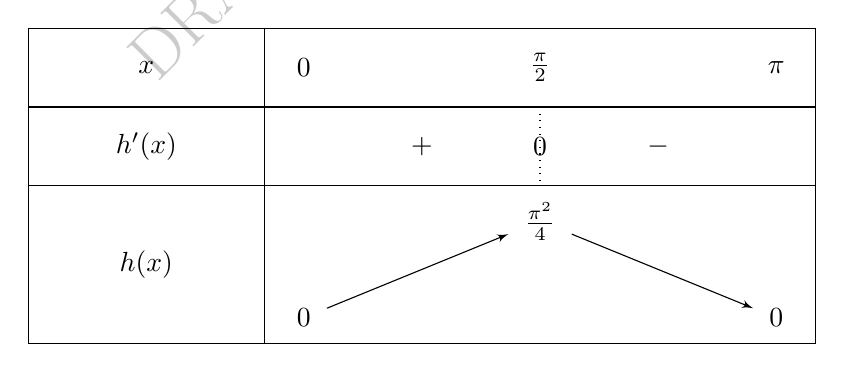
\begin{tikzpicture} 
\tkzTabInit[lgt=3, espcl=3]{$x$ /1, $h'(x)$ /1, $h(x)$ /2}{$0$, $\frac{\pi}{2}$, $\pi$} 
\tkzTabLine{, +, z, -,} 
\tkzTabVar{-/ $0$, +/ $\frac{\pi^2}{4}$ , -/ $0$}
\end{tikzpicture} 
\end{center}

\medskip
\underline{Graphe de $h$}
 
 
 

 


2) Calcul des coefficients de Fourier

La fonction \( h(x) = x(\pi - x) \) est impaire et \( 2\pi \)-périodique. Comme elle est impaire, tous les coefficients \( a_n \) (cosinus) sont nuls. On calcule uniquement les coefficients \( b_n \) (sinus) :

\[
b_n = \frac{2}{\pi} \int_0^\pi h(x) \sin(nx) \, dx.
\]

En remplaçant \( h(x) = x(\pi - x) \), on a :

\[
b_n = \frac{2}{\pi} \int_0^\pi x(\pi - x) \sin(nx) \, dx.
\]

On décompose l'intégrale :

\[
b_n = \frac{2}{\pi} \left( \pi \int_0^\pi x \sin(nx) \, dx - \int_0^\pi x^2 \sin(nx) \, dx \right).
\]

\textbf{Calcul des intégrales}

Première intégrale

\[
\int_0^\pi x \sin(nx) \, dx = \left[ -\frac{x \cos(nx)}{n} \right]_0^\pi + \frac{1}{n} \int_0^\pi \cos(nx) \, dx = \frac{(-1)^{n+1} \pi}{n}.
\]

Deuxième intégrale

\[
\int_0^\pi x^2 \sin(nx) \, dx = \left[ -\frac{x^2 \cos(nx)}{n} \right]_0^\pi + \frac{2}{n} \int_0^\pi x \cos(nx) \, dx.
\]

En utilisant le résultat de la première intégrale, on trouve :

\[
\int_0^\pi x^2 \sin(nx) \, dx = \frac{(-1)^{n+1} \pi^2}{n} + \frac{2}{n} \cdot \frac{(-1)^n - 1}{n^2}.
\]

\textbf{Combinaison des résultats}

En combinant les résultats, on obtient :

\[
b_n = \frac{2}{\pi} \left( \pi \cdot \frac{(-1)^{n+1} \pi}{n} - \left( \frac{(-1)^{n+1} \pi^2}{n} + \frac{2((-1)^n - 1)}{n^3} \right) \right).
\]

Après simplification, on trouve :

\[
b_n = \frac{4((-1)^n - 1)}{\pi n^3}.
\]


3) Développement en série de Fourier

Le développement en série de Fourier de \( h(x) \) est :

\[
h(x) = \sum_{n=1}^\infty b_n \sin(nx),
\]

avec \( b_n = \frac{4((-1)^n - 1)}{\pi n^3} \). On peut écrire :

\[
h(x) = \sum_{n=1}^\infty \frac{4((-1)^n - 1)}{\pi n^3} \sin(nx).
\]

4) Calcul des sommes \( S_1 \) et \( S_2 \)

\textbf{Calcul de \( S_1 = \sum_{n=0}^\infty \frac{(-1)^n}{(2n+1)^3} \)}

On utilise le développement en série de Fourier de \( h(x) \) en \( x = \frac{\pi}{2} \). On a :

\[
h\left(\frac{\pi}{2}\right) = \frac{\pi}{2} \left(\pi - \frac{\pi}{2}\right) = \frac{\pi^2}{4}.
\]

D'autre part, en évaluant la série de Fourier en \( x = \frac{\pi}{2} \), on obtient :

\[
h\left(\frac{\pi}{2}\right) = \sum_{n=1}^\infty b_n \sin\left(n \cdot \frac{\pi}{2}\right).
\]

Comme \( \sin\left(n \cdot \frac{\pi}{2}\right) \) vaut \( 0 \) pour \( n \) pair et \( (-1)^k \) pour \( n = 2k + 1 \), on a :

\[
\frac{\pi^2}{4} = \sum_{k=0}^\infty b_{2k+1} (-1)^k.
\]

En remplaçant \( b_{2k+1} \), on trouve :

\[
\frac{\pi^2}{4} = \sum_{k=0}^\infty \frac{4((-1)^{2k+1} - 1)}{\pi (2k+1)^3} (-1)^k.
\]

Simplification :

\[
\frac{\pi^2}{4} = \sum_{k=0}^\infty \frac{4(-2)}{\pi (2k+1)^3} (-1)^k = -\frac{8}{\pi} \sum_{k=0}^\infty \frac{(-1)^k}{(2k+1)^3}.
\]

On en déduit :

\[
S_1 = \sum_{k=0}^\infty \frac{(-1)^k}{(2k+1)^3} = -\frac{\pi^3}{32}.
\]

\textbf{Calcul de \( S_2 = \sum_{n=0}^\infty \frac{1}{(2n+1)^6} \)}

On utilise l'identité de Parseval pour la série de Fourier de \( h(x) \). L'identité de Parseval donne :

\[
\frac{1}{\pi} \int_{-\pi}^\pi h(x)^2 \, dx = \sum_{n=1}^\infty b_n^2.
\]

Comme \( h(x) \) est impaire, on a :

\[
\int_{-\pi}^\pi h(x)^2 \, dx = 2 \int_0^\pi h(x)^2 \, dx.
\]

Calcul de \( \int_0^\pi h(x)^2 \, dx \) :

\[
\int_0^\pi x^2 (\pi - x)^2 \, dx = \int_0^\pi x^2 (\pi^2 - 2\pi x + x^2) \, dx = \pi^2 \int_0^\pi x^2 \, dx - 2\pi \int_0^\pi x^3 \, dx + \int_0^\pi x^4 \, dx.
\]

En calculant chaque intégrale, on trouve :

\[
\int_0^\pi h(x)^2 \, dx = \frac{\pi^5}{30}.
\]

Ainsi, l'identité de Parseval donne :

\[
\frac{1}{\pi} \cdot 2 \cdot \frac{\pi^5}{30} = \sum_{n=1}^\infty b_n^2.
\]

Simplification :

\[
\frac{\pi^4}{15} = \sum_{n=1}^\infty \left( \frac{4((-1)^n - 1)}{\pi n^3} \right)^2 = \frac{16}{\pi^2} \sum_{n=1}^\infty \frac{((-1)^n - 1)^2}{n^6}.
\]

Comme \( ((-1)^n - 1)^2 = 4 \) pour \( n \) impair et \( 0 \) pour \( n \) pair, on a :

\[
\frac{\pi^4}{15} = \frac{16}{\pi^2} \cdot 4 \sum_{k=0}^\infty \frac{1}{(2k+1)^6}.
\]

On en déduit :

\[
S_2 = \sum_{k=0}^\infty \frac{1}{(2k+1)^6} = \frac{\pi^6}{960}.
\]






\medskip\textbf{Exercice 3}


\medskip
\textbf{Session 2020}

\medskip\textbf{Exercice 1}

On donne la matrice $ A= \begin{pmatrix}
1 & 0 & -1\\
0 & 1 & 0\\
-1 & 1 & 1
\end{pmatrix}$                                                                   

1. Justifions que la matrice $A$ est inversible.

$det(A)=\begin{vmatrix}
1 & 0 & -1\\
0 & 1 & 0\\
-1 & 1 & 1
\end{vmatrix}=1-1=0$, alors $A$ n'est pas inversible.

2. Déterminons le polynôme caractéristique de $A$.

$P_A(x)=det(A-xI_3)=\begin{vmatrix}
1-x & 0 & -1\\
0 & 1-x & 0\\
-1 & 1 & 1-x
\end{vmatrix}=(1-x)\begin{vmatrix}
1-x & -1 \\ 
-1 & 1-x
\end{vmatrix}$

$=(1-x)((1-x)^2-1)=(1-x)(1-x-1)(1-x+1)=-x(1-x)(2-x)$ 

3. Soit $\alpha, \beta$ et $\gamma$ les valeurs propres de la matrice $A$. Déterminons $\alpha, \beta$ et $\gamma$ sachant qu'elles sont classées dans l'ordre croissant.

$\alpha=0$, $\beta=1$ et $\gamma=2$


4. Déterminons les vecteurs propres $u$, $v$ et $w$ associés aux valeurs propres $\alpha$, $\beta$ et $\gamma$.

Soit $E_\lambda$ le sous-espace propre lié à la valeur propre $\lambda$

\[
E_\lambda=\{u\in \mathbb{R}^3/Au=\lambda u\}
\]

\medskip
$\bullet$ Pour $\lambda=\alpha=0$, on a :

$\forall u\in E_\alpha$, \[Au=0\Rightarrow \begin{pmatrix}
1 & 0 & -1\\
0 & 1 & 0\\
-1 & 1 & 1
\end{pmatrix}\begin{pmatrix}
x\\
y\\
z
\end{pmatrix}=\begin{pmatrix}
0\\
0\\
0
\end{pmatrix}\Rightarrow \begin{cases}
x-z=0(1)\\
y=0(2)\\
-x+y+z=0(3)
\end{cases}\]

$(1)\Rightarrow x=z \hspace{0.7cm} (4)$

$(2)\Rightarrow y=0$

D'où $u=\begin{pmatrix}
x\\
y\\
z
\end{pmatrix}=\begin{pmatrix}
x\\
0\\
x
\end{pmatrix}=x\begin{pmatrix}
1\\
0\\
1
\end{pmatrix}\Rightarrow E_2=\langle \begin{pmatrix}
1\\
0\\
1
\end{pmatrix}\rangle$ et $u=\begin{pmatrix}
1\\
0\\
1
\end{pmatrix}$

\medskip
$\bullet$ Pour $\lambda=\beta=1$, on a :

$\forall v\in E_\beta$, \[Av=v\Rightarrow \begin{pmatrix}
1 & 0 & -1\\
0 & 1 & 0\\
-1 & 1 & 1
\end{pmatrix}\begin{pmatrix}
x\\
y\\
z
\end{pmatrix}=\begin{pmatrix}
x\\
y\\
z
\end{pmatrix}\Rightarrow \begin{cases}
x-z=x(1)\\
y=y(2)\\
-x+y+z=z(3)
\end{cases}\]

$(1)\Rightarrow z=0 \hspace{0.7cm} (4)$

$(3)\Rightarrow y=x$

D'où $u=\begin{pmatrix}
x\\
y\\
z
\end{pmatrix}=\begin{pmatrix}
x\\
x\\
0
\end{pmatrix}=x\begin{pmatrix}
1\\
1\\
0
\end{pmatrix}\Rightarrow E_\beta=\langle \begin{pmatrix}
1\\
1\\
0
\end{pmatrix}\rangle$ et $v=\begin{pmatrix}
1\\
1\\
0
\end{pmatrix}$

$\bullet$ Pour $\lambda=\gamma=2$, on a :

$\forall w\in E_\beta$, \[Aw=2w\Rightarrow \begin{pmatrix}
1 & 0 & -1\\
0 & 1 & 0\\
-1 & 1 & 1
\end{pmatrix}\begin{pmatrix}
x\\
y\\
z
\end{pmatrix}=2\begin{pmatrix}
x\\
y\\
z
\end{pmatrix}\Rightarrow \begin{cases}
x-z=2x\\
y=2y\\
-x+y+z=2z0
\end{cases}\]

$(1)\Rightarrow z=-x \hspace{0.7cm} (4)$

$(2)\Rightarrow y=0$

D'où $w=\begin{pmatrix}
x\\
y\\
z
\end{pmatrix}=\begin{pmatrix}
x\\
0\\
-x
\end{pmatrix}=x\begin{pmatrix}
1\\
0\\
-1
\end{pmatrix}\Rightarrow E_2=\langle \begin{pmatrix}
1\\
0\\
-1
\end{pmatrix}\rangle$ et $w=\begin{pmatrix}
1 \\
0 \\
-1
\end{pmatrix}$


5. Soit $D=\begin{pmatrix}
\alpha & 0 & 0 \\ 
0 & \beta & 0 \\ 
0 & 0 & \gamma
\end{pmatrix} $.

Donnons la matrice de passage $P$ de $A$ à $D$.

$P=\begin{pmatrix}
1 & 1 & 1  \\ 
0 & 1 & 0  \\ 
1 & 0 & -1
\end{pmatrix}$

\medskip
\textbf{Exercice 2}

1. On considère la fonction $f$ définie sur $\mathbb{R}$ par $f(x)=e^{-x}$.


a. Montrer que $f$ est dérivable sur $\mathbb{R}$.

$f$ est définie, continue et dérivable sur sont domaine de définition qui est $\mathbb{R}$


b. Déterminons $f^\prime(x)$, $f^{\prime\prime}(x)$ et $f^{(3)}(x)$; $\forall {x}\in \mathbb{R}$.

$\forall {x}\in \mathbb{R}$,

$f^\prime(x)=-e^{-x}$

$f^{\prime\prime}(x)=e^{-x}$

$f^{(3)}(x)=-e^{-x}$



c. Démontrons par récurrence que : $f^{(n)}(x)=(-1)^ne^{-x}$

-Pour $n=0$, $f^{(0)}(x)=(-1)^0e^{-x}=e^{-x}=f(x)$ (vraie)

-Pour $n=1$, $f^{(1)}(x)=(-1)^1e^{-x}=-e^{-x}=f'(x)$ (vraie)

-Pour $n=2$, $f^{(2)}(x)=(-1)^2e^{-x}=e^{-x}=f''(x)$ (vraie)

-Supposons que $f^{(n)}(x)=(-1)^ne^{-x}$ est vraie à l'ordre $n$ et vérifions à l'ordre $n+1$.

$f^{(n)}(x)=(-1)^ne^{-x}\Rightarrow (f^{(n)}(x))^\prime=((-1)^ne^{-x})^\prime=-(-1)^ne^{-x}=(-1)^{n+1}e^{-x}$ avec $(f^{(n)}(x))^\prime=f^{(n+1)}(x)$, alors $f^{(n+1)}(x)=(-1)^{n+1}e^{-x}$, d'où la propriété est vraie à l'ordre $n+1$.

On conclut donc que $f^{(n)}(x)=(-1)^ne^{-x}$, $\forall n\in \mathbb{N}$

d. Donnons le développement limité d'ordre $n$ de $f$ au voisinage de $0$.

De la formule de Taylor, le développement limité d'ordre $n$ d'une fonction $f$ au voisinage de $x_0$ est donné par :

\[
f(x)=\sum_{k=0}^{n}\frac{(x-x_0)^k}{k!}f^{(k)}(x_0)+\tau(x^n)
\]

Dans notre cas, $x_0=0$

$f^{(n)}(x)=(-1)^ne^{-x}\Rightarrow f^{(n)}(0)=(-1)^ne^{-0}=(-1)^n$

Donc,
\begin{align*}
f(x)&=\sum_{k=0}^{n}\frac{(x-0)^k}{k!}f^{(k)}(0)+\circ(x^n)\\
&=\sum_{k=0}^{n}\frac{x^k}{k!}(-1)^k+\circ(x^n)\\
&=\sum_{k=0}^{n}(-1)^k\frac{x^k}{k!}+\circ(x^n)\\
f(x)&=1-\frac{x}{1!}+\frac{x^2}{2!}+\cdots (-1)^n\frac{x^n}{n!}+\circ(x^n)
\end{align*}

2. On considère la courbe paramétrée : $(\Gamma) :\begin{cases}
x(t)=\cos 3t\\
y(t)=\sin 2t
\end{cases} \forall t\in \mathbb{R}$

a. Montrons que l'étude de la courbe peut être réduite à l'intervalle $[0,\pi]$.

\textbf{Vérifions la périodicité}

On sait que $\cos(at)$ est périodique de période $\frac{2\pi}{\vert a\vert}$, et $\sin(bt)$ est périodique de période $\frac{2\pi}{\vert b\vert}$

Donc, $\cos(3t)$ est périodique de période $\frac{2\pi}{3}$ et $\sin(2t)$ est périodique de période $\pi$

Le $PPCM(\frac{2\pi}{3},\pi)=2\pi$ , donc la courbe est périodique de période $2\pi$. Ainsi, le domaine d'étude de la courbe peut être réduit à un intervalle d'amplitude $2\pi$, soit $[-\pi,\pi]$

\medskip
\textbf{Vérifions la parité}

$\begin{cases}
x(-t)=\cos(-3t)=\cos 3t=x(t)\\
y(-t)=\sin(-2t)=-\sin 2t=-y(t)
\end{cases}$

$x(t)$ est paire et $y(t)$ est impaire, alors la courbe est symétrique par rapport à l'axe des abscisses. Donc le domaine d'étude de la courbe peut être réduit à $[0,\pi]$.

b. Dressons le tableau de variation commun de $x$ et $y$ sur $[0,\pi]$.

Étudions la courbe.

\textbf{Étude de $x(t)$}

$x(t)=\cos 3t$ est définie, continue et dérivable sur $\mathbb{R}$, car fonction trigonométrique, et

$x'(t)=-3\sin 3t$

\medskip
Signe de $x'(t)$

soit $x'(t)=-3\sin 3t=0\Rightarrow \sin 3t=0=\sin 0\Rightarrow \begin{cases}
3t=2k\pi\\
3t=\pi+2k\pi
\end{cases}\Rightarrow \begin{cases}
t=\frac{2k\pi}{3}\\
t=\frac{\pi}{3}+\frac{2k\pi}{3}
\end{cases}\forall k\in \mathbb{Z}$

-Pour $k=0, t=0$ ou $t=\frac{\pi}{3}$

-Pour $k=1,t=\frac{2\pi}{3}$ ou $t=\pi$

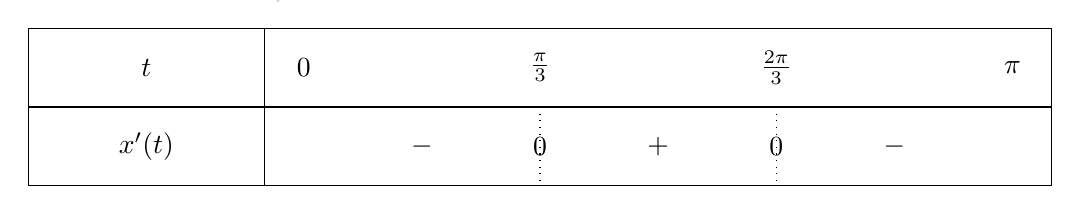
\begin{tikzpicture}
  \tkzTabInit[lgt=3, espcl=3]{$t$ /1, $x'(t)$ /1}{$0$, $\frac{\pi}{3}$, $\frac{2\pi}{3}$, $\pi$}
  \tkzTabLine{, -, z, +, z, -,}
\end{tikzpicture}


\underline{Variations de $x(t)$}

\[
\begin{cases}
\forall t\in [0,\frac{\pi}{3}],x'(t)\leq 0\hspace*{0.5cm} alors\hspace*{0.5cm} x(t)\hspace*{0.5cm} est \hspace*{0.5cm}decroissante\\
\forall t\in [\frac{\pi}{3}, \frac{2\pi}{3}], x'(t)\geq 0 \hspace*{0.5cm} alors\hspace*{0.5cm} x(t)\hspace*{0.5cm} est\hspace*{0.5cm} croissante\\
\forall t\in [\frac{2\pi}{3},\pi], x'(t)\leq 0\hspace*{0.5cm} alors\hspace*{0.5cm} x(t)\hspace*{0.5cm} est\hspace*{0.5cm} decroissante
\end{cases}
\]

\medskip\textbf{Étude de $y(t)$ sur $[0,\pi]$}

$y(t)=\sin{2t}\Rightarrow y'(t)=2\cos 2t$

$y'(t)=0\Rightarrow \cos 2t=0=\cos\frac{\pi}{2}$

\[
\begin{cases}
2t=\frac{\pi}{2}+2k\pi\\
2t=-\frac{\pi}{2}+2k\pi
\end{cases}\Rightarrow
\begin{cases}
t=\frac{\pi}{4}+k\pi\\
t=-\frac{\pi}{4}+k\pi
\end{cases}
\]

-Pour $k=0$, $t=\frac{\pi}{4}$

-Pour $k=1$, $t=\frac{3\pi}{4}$

Tableau de signe de $y'(t)$

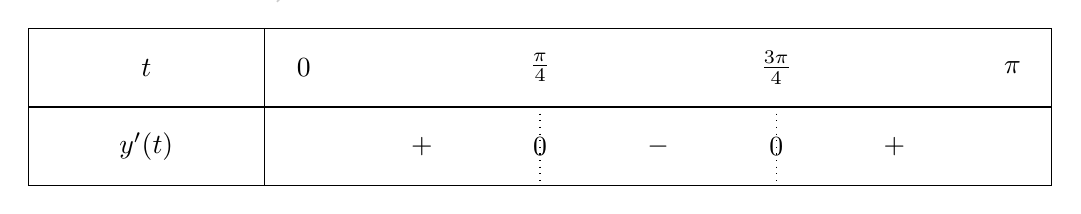
\begin{tikzpicture}
  \tkzTabInit[lgt=3, espcl=3]{$t$ /1, $y'(t)$ /1}{$0$, $\frac{\pi}{4}$, $\frac{3\pi}{4}$, $\pi$}
  \tkzTabLine{, +, z, -, z, +,}
\end{tikzpicture}

\underline{Variations de $y(t)$}

\[
\begin{cases}
\forall t\in [0,\frac{\pi}{4}],y'(t)\geq 0\hspace*{0.5cm} alors\hspace*{0.5cm} y(t)\hspace*{0.5cm} est \hspace*{0.5cm}croissante\\
\forall t\in [\frac{\pi}{4}, \frac{3\pi}{4}], y'(t)\leq 0 \hspace*{0.5cm} alors\hspace*{0.5cm} y(t)\hspace*{0.5cm} est\hspace*{0.5cm} decroissante\\
\forall t\in [\frac{3\pi}{4},\pi], y'(t)\leq 0\hspace*{0.5cm} alors\hspace*{0.5cm} y(t)\hspace*{0.5cm} est\hspace*{0.5cm} croissante
\end{cases}
\]

\medskip\textbf{Tableau commun de variation des fonctions $x$ et $y$}

$x(0)=1$, $x(\frac{\pi}{4})=-\frac{\sqrt{2}}{2}$, $x(\frac{\pi}{3})=-1$, $x(\frac{2\pi}{3})=1$, $x(\frac{3\pi}{4})=-1$, $x(\pi)=-1$

$x'(0)=0$, $x'(\pi)=0$

$y(0)=0$, $y(\frac{\pi}{4})=1$, $y(\frac{\pi}{3})=\frac{\sqrt{3}}{2}$, $y(\frac{2\pi}{3})=-\frac{\sqrt{3}}{2}$, $y(\frac{3\pi}{4})=-1$, $y(\pi)=0$

$y'(0)=2$, $y'(\pi)=2$

\begin{center}
\resizebox{\textwidth}{!}{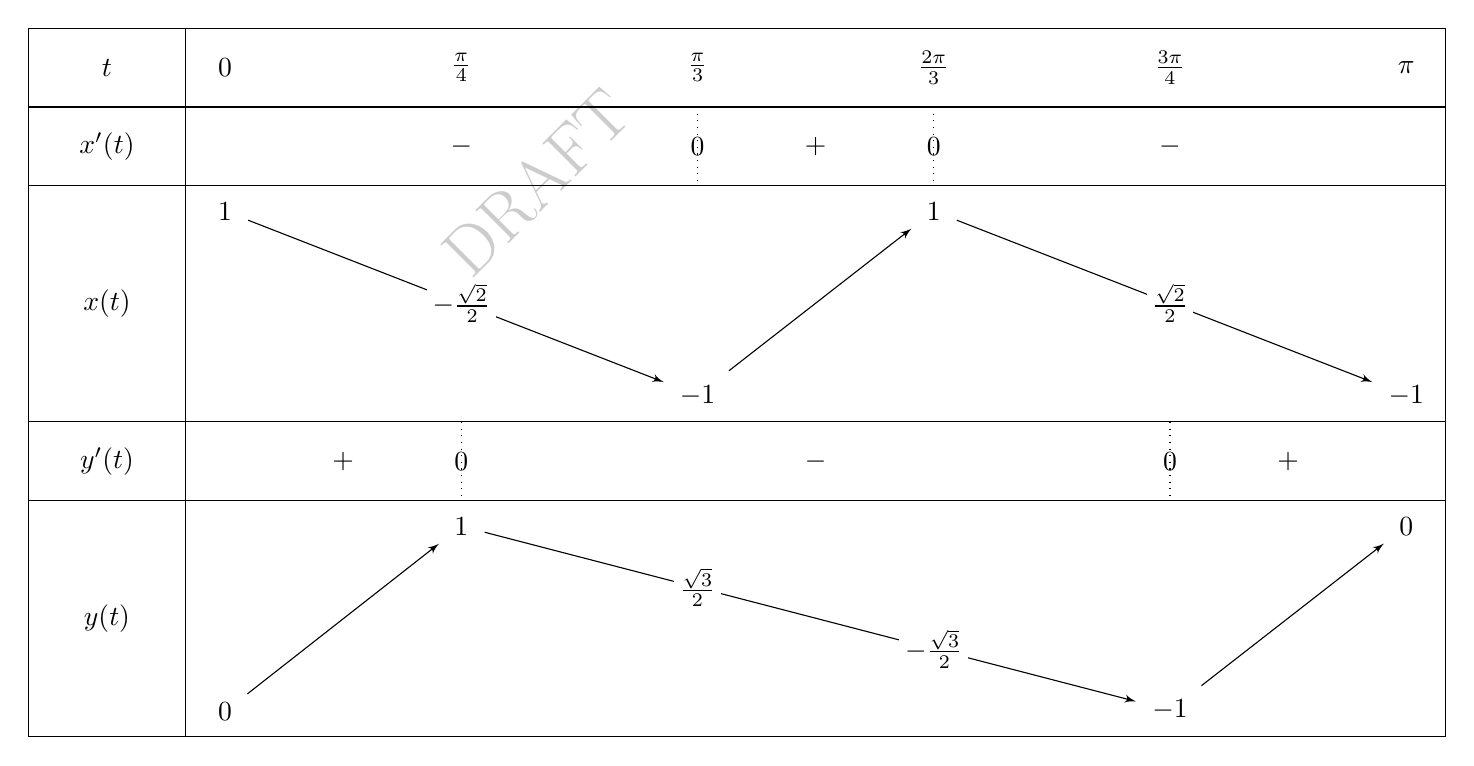
\begin{tikzpicture}
    % Initialisation du tableau
    \tkzTabInit[lgt=2, espcl=3]
    {$t$ /1, $x'(t)$ /1, $x(t)$ /3, $y'(t)$ /1, $y(t)$ /3} 
    {$0$, $\frac{\pi}{4}$, $\frac{\pi}{3}$, $\frac{2\pi}{3}$, $\frac{3\pi}{4}$, $\pi$}

    % Ligne de signes de x'(t)
    \tkzTabLine{, ,-, ,z, +,z, ,- ,}
    
    
    % Ligne de variations de x(t)
    \tkzTabVar{+/$1$, R/ , -/$-1$, +/$1$, R/, -/$-1$,}
    
    %Pour mettre des valeurs(les images) sur les flèches
    \tkzTabIma{1}{3}{2}{$-\frac{\sqrt{2}}{2}$}
    
    \tkzTabIma{4}{6}{5}{$\frac{\sqrt{2}}{2}$}
    % Ligne de signes de y'(t)
    
    % Ligne de signes de y'(t)
    \tkzTabLine{,+,z, , ,- , , ,z,+}
    
    %Pour ajouter les valeurs de dérivées(vecteurs directeurs)
    
    
    % Ligne de variations de y(t)
    \tkzTabVar{-/$0$, +/$1$, R/ , R/ , -/$-1$, +/$0$,}
    
    %Pour mettre des valeurs (les images) sur les flèches.
    \tkzTabIma{2}{5}{3}{$\frac{\sqrt{3}}{2}$}
    
    \tkzTabIma{2}{5}{4}{$-\frac{\sqrt{3}}{2}$}
\end{tikzpicture}
}
\end{center} 

\medskip
\textbf{Exercice 3}

Soient $n\geq 1$, un entier naturel et $\mathbb{R}_n[X]$ l'espace vectoriel des polynômes réels de degré inférieur ou égal à $n$. $\forall {P,Q\in \mathbb{R}_n[x]}$, on pose :

\[ \beta(P,Q)=\int_{0}^{1}xP(x)Q^{\prime}(x). dx\]

1. Montrons que $\beta$ est une forme bilinéaire.

\underline{Montrons que $\beta$ est linéaire par rapport à la première variable}

Soient $P,Q$ et $G$ $\in \mathbb{R}_n[x]$ et $\alpha\in \mathbb{R}$

On a :

\begin{align*}
\beta(P+\alpha G,Q) &=\int_{0}^{1}x(P(x)+\alpha G(x)) Q^{\prime}(x).dx\\
&=\int_{0}^{1}(xP(x)Q^{\prime}(x)+\alpha xG(x)Q^{\prime}(x)).dx\\
&=\int_{0}^{1}xP(x)Q^{\prime}(x).dx+\alpha\int_{0}^{1}xG(x)Q^{\prime}(x).dx\\
\beta(P+\alpha G,Q) &=\beta(P,Q)+\alpha\beta(G,Q)
\end{align*}, alors $\beta$ est linéaire par rapport à la première variable.

 \medskip
 \underline{Montrons que $\beta$ est linéaire par rapport à la deuxième variable}
 
 Soient $P,Q$ et $G$ $\in \mathbb{R}_n[x]$ et $\alpha\in \mathbb{R}$
 
 On a :

\begin{align*}
\beta(P,\alpha G+Q)&=\int_{0}^{1}xP(x)(\alpha G + Q)^{\prime}(x). dx\\
&=\int_{0}^{1}xP(x)(\alpha G^{\prime}(x) + Q^{\prime}(x)). dx\\
&=\alpha\int_{0}^{1}xP(x)G^{\prime}(x).dx+\int_{0}^{1}xP(x)Q^{\prime}(x). dx\\
\beta(P,\alpha G+Q)&=\alpha\beta(P,G)+\beta(P,Q)
\end{align*}, alors $\beta$ est linéaire par rapport à la deuxième variable.

On conclut donc que $\beta$ est \textbf{bilinéaire}.
 

2. Exprimons $\beta(x,1)$ et $\beta(1,x)$.

$\beta(x,1)=\int_{0}^{1}x\times x\times 1^{\prime}. dx=\int_{0}^{1}x^2\times 0.dx =0$

$\beta(1,x)=\int_{0}^{1}x\times 1\times(x)^{\prime}. dx=\int_{0}^{1}x=[\frac{1}{2}x^2]_0^1=\frac{1}{2}$

3. $\beta$ est-elle symétrique? Antisymétrique?

$\beta$ est symétrique si $\beta(P,Q)=\beta(Q,P)$.

On a : $\beta(x,1)\neq\beta(1,x)$ alors $\beta$ n'est pas symétrique, mais antisymétrique.


\medskip
\textbf{Exercice 4}

1. Montrer à l'aide du théorème de Fubini que : 

$I=\int_{0}^{+\infty}e^{-\frac{x^2}{2}}dx=\sqrt{\frac{\pi}{2}}$

$I=\int_{0}^{+\infty}e^{-\frac{x^2}{2}}dx\Longrightarrow I^2=(\int_{0}^{+\infty}e^{-\frac{x^2}{2}}dx)^2=(\int_{0}^{+\infty}e^{-\frac{x^2}{2}}dx)\times (\int_{0}^{+\infty}e^{-\frac{y^2}{2}}dy)=\int_{0}^{+\infty}\int_{0}^{+\infty}e^{-\frac{x^2}{2}}\times e^{-\frac{y^2}{2}}dxdy=\int_{0}^{+\infty}\int_{0}^{+\infty}e^{-\frac{x^2+y^2}{2}}dxdy$

\medskip
Posons :

$\begin{cases}
x=r\cos\theta\\
y=r\sin\theta
\end{cases}$

$x^2+y^2=r^2$

\medskip
Calculons le Jacobien

$J(r,\theta)=\begin{vmatrix}
\frac{\partial x}{\partial r}&\frac{\partial x}{\partial \theta}\\
\frac{\partial y}{\partial r} & \frac{\partial y}{\partial \theta}
\end{vmatrix}=\begin{vmatrix}
\cos\theta & -r\sin\theta\\
\sin\theta & r\cos\theta
\end{vmatrix}=r$ $\Rightarrow dxdy=rdrd\theta$

Si $x\longrightarrow 0$ et $y\longrightarrow 0$ alors $r\longrightarrow 0$

Si $x\longrightarrow +\infty$ et $y\longrightarrow +\infty$ alors $r\longrightarrow +\infty$, mais de sorte que $cos\theta$ et $sin\theta$ soient positifs( donc $\theta\in [0,\frac{\pi}{2}]$).

Ainsi $r\in [0, +\infty[$ et $\theta\in [0,\frac{\pi}{2}]$

Donc, 

\[
I^2=\int_0^{+\infty}\int_0^{\frac{\pi}{2}}e^{-\frac{r^2}{2}}rdrd\theta=\int_0^{+\infty}re^{-\frac{r^2}{2}}dr\times \int_0^{\frac{\pi}{2}}d\theta=[-e^{-\frac{r^2}{2}}]_0^{+\infty}\times [\theta]_0^{\frac{\pi}{2}}=1\times \frac{\pi}{2}=\frac{\pi}{2}\]

$I^2=\frac{\pi}{2}$ Comme $I\geq 0$ alors $I=\sqrt{\frac{\pi}{2}}$


2. On pose $\forall {n\in \mathbb{N}}$, $\forall {x\in \mathbb{R}}$ $\\
f_n(x)=(1+\frac{x^2}{n})-\frac{n+1}{2}$ et $a_n=\int_{-\infty}^{+\infty}f_n(x)dx.$

a. Montrons que, $\forall {u\in \mathbb{R}}$ et $\forall {p\in \mathbb{N}}, (1+u)^p\geq 1+pu$.

Procédons par récurrence :

-Pour $p=1$, on a $(1+u)^1\geqslant 1+u$ (vrai)

-Pour $p=2$, on a $(1+u)^2=1+2u+u^2\geq 1+2u$ (vrai)

-Supposons que $(1+u)^p\geq 1+pu$ est vrai à l'ordre $p$, et vérifions à l'ordre $p+1$.

On a :

$(1+u)^p\geq 1+pu\Rightarrow (1+u)^p(1+u)\geq (1+pu)(1+u)\Rightarrow (1+u)^{p+1}\geq 1+pu + u+pu^2\Rightarrow (1+u)^{p+1}\geq 1+pu + u+pu^2$ avec $1+pu + u+pu^2=1+(1+p)u+pu^2\geq 1+(1+p)u$.

$\Rightarrow (1+u)^{p+1}\geq 1+(1+p)u$, d'où la propriété est vraie à l'ordre $p+1$.

On conclut donc que la propriété est vraie $\forall {u\in \mathbb{R}}$ et $\forall {p\in \mathbb{N}}$.


b. Déduisons que $\forall {x\in \mathbb{R}}, f_n(x) \leq \frac{2}{1+x^2}$.

On a  $f_n(x)=(1+\frac{x^2}{n})-\frac{n+1}{2}$ 

$(1+u)^p\geq 1+pu\Longrightarrow (1+u)^{-p}\leq \frac{1}{1+pu}$

De plus, $\frac{1}{1+pu}\leq \frac{2}{1+pu}\Longrightarrow (1+u)^{-p}\leq \frac{2}{1+pu}$

Posons $p=\frac{n+1}{2}$ et $u=\frac{x^2}{n}$

En reportant dans l'équation précédente, on obtient : 

$f_n(u)=(1+u)^{-p}$ et $f_n(x)\leq\frac{2}{1+x^2}$

c. Calculons $lim_{n\to +\infty}a_n$.

$lim_{n\to +\infty}a_n=lim_{n\to +\infty}\int_{-\infty}^{+\infty}f_n(x)dx\leq \lim_{n\to +\infty}\int_{-\infty}^{+\infty}\frac{2}{1+x^2}=\lim_{n\to +\infty}[2\arctan(x)]_{-\infty}^{+\infty}=\lim_{n\to +\infty}2(\frac{\pi}{2}+\frac{\pi}{2})=2\pi$

$\Longrightarrow lim_{n\to +\infty}a_n=2\pi$

\medskip
\textbf{Session 2021}

\textbf{Exercice 1}

Étudions la nature(convergente ou divergente) des séries numériques suivantes : 

\[\bullet S_1=\sum^{+\infty}_{n=1}(1-\frac{1}{n})^n\]

Soit $u_n=(1-\frac{1}{n})^n\Longrightarrow S_1=\sum^{+\infty}_{n=1}u_n$

Calculons la limite de $u_n$

On a :

$u_n=(1-\frac{1}{n})^n=e^{nln(1-\frac{1}{n})}$

Si $n\longrightarrow +\infty$ alors $-\frac{1}{n}\longrightarrow 0$ et $ln(1-\frac{1}{n})\sim -\frac{1}{n}+\circ(\frac{1}{n})$ (Développement limité de Taylor)


Ainsi,

 \[\lim_{n\to +\infty} u_n=\lim_{n\to +\infty}e^{n(-\frac{1}{n}+\circ(\frac{1}{n}))}=\lim_{n\to +\infty}e^{-1+\circ(1)}\longrightarrow \frac{1}{e}\neq 0\] alors $S_1$ diverge.

\medskip
\[\bullet S_2=\sum^{+\infty}_{n=1}\frac{n(n-1)}{(n+1)!}\].

Soit $u_n=\frac{n(n-1)}{(n+1)!}\Rightarrow u_{n+1}=\frac{n(n+1)}{(n+2)!}$

On a : 
\begin{align*}
\lim_{n\to +\infty}\frac{u_{n+1}}{u_n} &=\lim_{n\to +\infty}\frac{\frac{n(n+1)}{(n+2)!}}{\frac{n(n-1)}{(n+1)!}}\\
&=\lim_{n\to +\infty}\frac{n(n+1)(n+1)!}{n(n-1)(n+2)!}\\
&=\lim_{n\to +\infty}\frac{n(n+1)(n+1)!}{n(n-1)(n+2)(n+1)!}\\
&=\lim_{n\to +\infty}\frac{n+1}{(n-1)(n+2)}=\lim_{n\to +\infty}\frac{n}{n^2}=\lim_{n\to +\infty}\frac{1}{n}=0<1
\end{align*}, alors $S_2$ converge d'après le critère d'Alembert.



\medskip
\textbf{Exercice 2 }



1 : Développement en série entière de la fonction \( u \)

On considère l'équation différentielle suivante :
\[
(x - 1) u'(x) + u(x) = 0,
\]
avec la condition initiale \( u(0) = -1 \). Nous cherchons le développement en série entière de la solution \( u(x) \).

\quad
 Résolution de l'équation différentielle

Nous réécrivons l'équation sous la forme :
\[
u'(x) = \frac{-u(x)}{x - 1}.
\]

Nous cherchons une solution sous la forme d'une série entière autour de \( x = 0 \), soit :
\[
u(x) = \sum_{n=0}^{\infty} a_n x^n.
\]

En dérivant cette série terme à terme, on obtient :
\[
u'(x) = \sum_{n=1}^{\infty} a_n n x^{n-1}.
\]

Nous remplaçons cette expression dans l'équation différentielle :
\[
(x - 1) \sum_{n=1}^{\infty} a_n n x^{n-1} + \sum_{n=0}^{\infty} a_n x^n = 0.
\]

\quad
 Développement des termes

Développons \( (x - 1) \) et multiplions la série par \( (x - 1) \). Nous obtenons :
\[
(x - 1) \sum_{n=1}^{\infty} a_n n x^{n-1} = \sum_{n=1}^{\infty} a_n n (x^{n} - x^{n-1}).
\]

Cela donne :
\[
\sum_{n=1}^{\infty} a_n n x^n - \sum_{n=1}^{\infty} a_n n x^{n-1}.
\]

En ajoutant la deuxième série \( \sum_{n=0}^{\infty} a_n x^n \), on obtient :
\[
\left( \sum_{n=1}^{\infty} a_n n x^n - \sum_{n=1}^{\infty} a_n n x^{n-1} \right) + \sum_{n=0}^{\infty} a_n x^n = 0.
\]

Nous réorganisons les indices et combinons les termes en \( x^n \), ce qui nous permet d'obtenir une relation de récurrence entre les coefficients \( a_n \).

\quad
 Résolution de la relation de récurrence

Nous trouvons la relation de récurrence suivante pour les coefficients \( a_n \) :
\[
a_n = \frac{1}{n} a_{n-1}, \quad \text{pour } n \geq 1.
\]

Nous utilisons la condition initiale \( u(0) = -1 \), ce qui donne \( a_0 = -1 \). En utilisant la relation de récurrence, nous pouvons calculer les autres coefficients :
\[
a_1 = \frac{1}{1} a_0 = -1, \quad a_2 = \frac{1}{2} a_1 = \frac{1}{2}, \quad a_3 = \frac{1}{3} a_2 = \frac{1}{6}, \quad \dots
\]

Ainsi, la série entière de la solution \( u(x) \) est :
\[
u(x) = \sum_{n=0}^{\infty} \frac{(-1)^n}{n!} x^n.
\]

Il s'agit du développement en série entière de la fonction \( u(x) \).

 2. Rayon de convergence de la série

Le rayon de convergence \( R \) de la série entière \( u(x) = \sum_{n=0}^{\infty} a_n x^n \) est donné par la formule de Cauchy-Hadamard :
\[
\frac{1}{R} = \limsup_{n \to \infty} \sqrt[n]{|a_n|}.
\]

Ici, nous avons \( a_n = \frac{(-1)^n}{n!} \), donc :
\[
\limsup_{n \to \infty} \sqrt[n]{|a_n|} = \limsup_{n \to \infty} \sqrt[n]{\frac{1}{n!}} = 0.
\]

Ainsi, le rayon de convergence est \( R = \infty \).

 3. Domaine de convergence

Étant donné que le rayon de convergence de la série est \( R = \infty \), cela signifie que la série converge pour tous les \( x \in \mathbb{R} \). Ainsi, le domaine de convergence de la série est \( \mathbb{R} \).



\medskip
\textbf{Exercice 3}

Calculons $\int\int_{D}f(x,y)dxdy$ dans les cas suivants :

1. $D= \lbrace {y\geq 0, x+y, y-x\leq 1\rbrace}$ et $f(x,y)=x^{2}y$.


On a:

$
\begin{cases}
x+y\leq 1 (1)\\
y-x \leq 1 (2)
\end{cases}$

$(1)+(2)\Longrightarrow 2y\leq 2 \Longrightarrow y\leq 1$

De plus, $y\geq 0$. 	D'où $0\leq y\leq 1\Rightarrow y\in [0,1]$

$
\begin{cases}
x+y\leq 1 \\
y-x \leq 1 
\end{cases}\Rightarrow 
\begin{cases}
x\leq 1-y \\
x \geq y-1
\end{cases}\Longrightarrow  y-1\leq x \leq 1-y \Rightarrow x\in [y-1,1-y]$

Donc,
$
\int\int_{D}f(x,y)dxdy=\int_0^1\int_{y-1}^{1-y}x^2ydxdy=\int_0^1(\int_{y-1}^{1-y}x^2y.dx)dy
$

$\int_{y-1}^{1-y}x^2y.dx=2\int_{0}^{1-y}x^2y.dx$ car $x\mapsto x^2y$ est une fonction paire pour $y$ fixée.

Donc

\begin{align*}
\int\int_{D}f(x,y)dxdy &=\int_0^1(2\int_{0}^{1-y}x^2ydx)dy\\
&=2\int_0^1([\frac{1}{3}x^3y]_0^{1-y})dy\\
&=\frac{2}{3}\int_0^1y(1-y)^3dy\\
&=\frac{2}{3}\int_0^1y(1-3y+3y^2-y^3)dy\\
&=\frac{2}{3}\int_0^1(y-3y^2+3y^3-y^4)dy\\
&=\frac{2}{3}[\frac{1}{2}y-y^3+\frac{3}{4}y^4-\frac{1}{5}y^5]_0^1\\
&=\frac{2}{3}(\frac{1}{2}-1+\frac{3}{4}-\frac{1}{5})\\
\int\int_{D}f(x,y)dxdy &=\frac{1}{30}
\end{align*}

\medskip
2. $D= \lbrace 0\leq y\leq x, x^2+y^2 \leq 1\rbrace$ et $f(x,y)=e^{x^2+y^2}$.

Posons :

$x=rcos\theta$ et $y=rsin\theta$

$x^2+y^2=r^2$

$x^2+y^2 \leq 1\Rightarrow r^2\leq 1\Longrightarrow 0\leq r \leq 1\Longrightarrow r\in [0,1]$

$0\leq y\leq x\Rightarrow 0\leq rsin\theta\leq rcos\theta\Rightarrow 0\leq sin\theta\leq cos\theta\\Rightarrow 0\leq \tan\theta\leq 1$. En appliquant $\arctan(x)$ à cette inégalité, on obtient :

$\arctan(0)\leq \arctan(\tan(\theta))\leq \arctan(1)\Longrightarrow 0\leq \theta\leq \frac{\pi}{4}\Longrightarrow \theta\in [0,\frac{\pi}{4}]$

Calculons le jacobien :

$j(r,\theta)=\begin{vmatrix}
\frac{\partial x}{\partial r} & \frac{\partial x}{\partial \theta}\\
\frac{\partial y}{\partial r} & \frac{\partial x}{\partial \theta}
\end{vmatrix}=\begin{vmatrix}
cos \theta & -r\sin\theta\\
\sin\theta & r\cos\theta
\end{vmatrix}=r\Rightarrow dxdy=rdrd\theta$

Donc,

\begin{align*}
\int\int_{D}f(x,y)dxdy &=\int_0^{\frac{\pi}{4}}\int_{0}^1e^{r^2}rdrd\theta\\
&=\int_0^{\frac{\pi}{4}}d\theta\times\int_{0}^1re^{r^2}dr\\
&=[\theta]_0^{\frac{\pi}{4}}\times[\frac{1}{2}e^{r^2}]_0^1\\
&=\frac{\pi}{4}\times\frac{1}{2}(e-1)=\frac{\pi}{8}(e-1)
\end{align*}

\medskip
\textbf{Exercice 4}

Soit l'équation différentielle

$(E) : y^{\prime\prime}-4y^{\prime} + 4y = (t^2 - 1)e^t$.

1. Trouvons une solution particulière de $(E)$ sous la forme $y_p= Q(t)e^t$ ou $Q$ est un polynôme de degré 2.

$y_p=(at^2+bt+c)e^t$

$y'_p=(2at+b)e^t+(at^2+bt+c)e^t=(at^2+(2a+b)t+b+c)e^t$

$y''_p=(2at+2a+b)e^t+(at^2+(2a+b)t+b+c)e^t=(at^2+(4a+b)t+2a+2b+c)e^t$

En reportant dans l'équation différentielle $(E)$, on obtient;

$(at^2+(4a+b)t+2a+2b+c)e^t-4(at^2+(2a+b)t+b+c)e^t+4(at^2+bt+c)e^t=(t^2 - 1)e^t$

$(at^2+(b-4a)t+(2a-2b+c))e^t=(t^2 - 1)e^t$

Par identification,

$\begin{cases}
a=1\\
b-4a=0\\
2a-2b+c=-1
\end{cases}\Rightarrow \begin{cases}
a=1\\
b=4\\
c=5
\end{cases}$

D'où $y_p=(t^2+4t+5)e^t$

2. Déduisons la solution générale de $(E)$.

Calculons la solution homogène :

L'équation homogène est donnée par :

$y^{\prime\prime}-4y^{\prime} + 4y =0$

L'équation caractéristique :

$r^2-4r+4=0\Rightarrow (r-2)^2=0\Rightarrow r_0=2$

On a une racine double, donc la solution homogène est de la forme :

$y_0=(At+B)e^{2t}$ avec $A,B\in \mathbb{R}$

Ainsi la solution générale est donnée par :

\[
y_G=y_0+y_p=(At+B)e^{2t}+(t^2+4t+5)e^t\] avec $A,B\in \mathbb{R}$


3. Trouvons la solution $h$ telle que $h(0)=h^{\prime}(0)=1$

$h(t)=(At+B)e^{2t}+(t^2+4t+5)e^t$

$h(0)=1\Rightarrow B+5=1\Rightarrow B=-4$

$h'(t)=Ae^{2t}+2(At+B)e^{2t}+(2t+4)e^t+(t^2+4t+5)e^t$

$h'(0)=1\Rightarrow A+2B+4+5=1\Rightarrow A+2B=-8\Rightarrow A=0$

$h(t)=-4e^{2t}+(t^2+4t+5)e^t$

\medskip
\textbf{Session 2022}

\textbf{Exercice 1 : (4pts)}

Soit la suite numérique $(U_n)$ définie sur $\mathbb{N}$ par : $U_0 = 2$ et $U_{n+1} = \frac{2}{3}U_n + \frac{1}{3}n + 1, \forall {n\in \mathbb{N}}$.
1.a. Démontrons que pour tout $n, U_n\leq n+3$.

Raisonnons par récurrence :

-Pour $n=0$, $U_0=2\leq 0+3=3$. La propriété est vrai pour $n=0$.

-Supposons que la propriété est vrai au rang $n$, et vérifions au rang $n+1$.

Par hypothèse :

$U_n\leq n+3\Rightarrow \frac{2}{3}U_n\leq 2(\frac{1}{3}n+1)\Rightarrow \frac{2}{3}U_n+\frac{1}{3}n + 1\leq 2(\frac{1}{3}n+1)+\frac{1}{3}n + 1\Rightarrow U_{n+1}\leq 3(\frac{1}{3}n + 1)\Rightarrow U_{n+1}\leq n+3$. Alors la propriété est vrai au rang $n+1$.

On conclut donc que, $\forall n\in \mathbb{N}, U_n\leq n+3$.


b. Démontrons que $\forall {n\in \mathbb{N}}, U_{n+1} - U_n = \frac{1}{3}(n+3-U_n)$.

\begin{align*}
U_{n+1} &= \frac{2}{3}U_n + \frac{1}{3}n + 1\\
U_{n+1}-U_n &= \frac{2}{3}U_n + \frac{1}{3}n + 1-U_n\\
&=\frac{1}{3}n + 1-\frac{1}{3}\\
U_{n+1}-U_n &=\frac{1}{3}(n + 3-U_n)
\end{align*}

c. Déduisons le sens de variation de la suite $(U_n)$.

$U_{n+1}-U_n =\frac{1}{3}(n + 3-U_n)$

D'après la question 1.a., $U_n\leq n+3\Rightarrow n + 3-U_n\geq 0 \Rightarrow \frac{1}{3}(n + 3-U_n)\geq 0\Rightarrow U_{n+1}-U_n \geq 0\Rightarrow U_{n+1}\geq U_n$ alors $U_n$ est croissante.

2. On désigne par $(V_n)$ la suite définie sur $\mathbb{N}$ par $V_n =U_n-n$.

a. Démontrons que la suite $(V_n)$ est une suite géométrique de raison $\frac{2}{3}$.

\begin{align*}
V_n =U_n-n\Rightarrow V_{n+1} &=U_{n+1}-n-1\\
&=\frac{2}{3}U_n + \frac{1}{3}n + 1-n-1\\
&=\frac{2}{3}U_n - \frac{2}{3}n\\
&=\frac{2}{3}(U_n-n)\\
V_{n+1} &=\frac{2}{3}V_n
\end{align*}, alors $(V_n)$ est une suite géométrique de raison $\frac{2}{3}$


b. Déduisons $\forall {n\in \mathbb{N}}$ que $U_n = 2(\frac{2}{3})^n + n$.

$(V_n)$ est une suite géométrique de raison $\frac{2}{3}$ et de premier terme $V_0=U_0=2$ alors l'expression de $V_n$ en fonction de $n$ est :

$V_n=V_0(\frac{2}{3})^n=2(\frac{2}{3})^n$

On a :

$V_n =U_n-n\Rightarrow U_n =V_n+n\Rightarrow U_n = 2(\frac{2}{3})^n + n$.


c. La suite $(U_n)$ est-elle convergente?

\[\lim_{n\to +\infty}U_n = \lim_{n\to +\infty}(2(\frac{2}{3})^n + n)=+\infty\]. Alors $U_n$ diverge.

\medskip
\textbf{Exercice 2}

Soit l'intégrale $I=\int_{0}^{1}\frac{\ln(1 + x)}{1 + x^2}dx$.

1. Montrons que $\forall {x\in ]-1,+\infty[}$, on a : $\ln(1+x) = \int_{0}^{1}\frac{x}{1 + xy}dy$.

Pour $x$ fixée, la fonction $y\longmapsto \frac{x}{1 + xy}$ est de la forme $\frac{u'}{u}$ avec $u(y)=1+xy$, alors : 

$\int_{0}^{1}\frac{x}{1 + xy}dy=[ln(1+xy)]_0^1=ln(1+x)-ln(1+0)=ln(1+x)$


Déduisons que $I = \int\int_D\frac{x}{(1+x^2)(1+xy)}dxdy$ ou  $D$ est le pavé $[0,1]^2$.


$I=\int_{0}^{1}\frac{\ln(1 + x)}{1 + x^2}dx$ avec $ln(1+x)=\int_{0}^{1}\frac{x}{1 + xy}dy$, donc 

$I=\int_{0}^{1}\frac{\int_{0}^{1}\frac{x}{1 + xy}dy}{1 + x^2}dx=\int_{0}^{1}\int_{0}^{1}\frac{1}{1 + x^2}\times\frac{x}{1 + xy}dxdy=\int\int_D\frac{x}{(1+x^2)(1+xy)}dxdy$ ou  $D$ est le pavé $[0,1]^2$.


2. Considérons $f(x)= \frac{x}{(1+x^2)(1+xy)}$ pour $y$ fixé.

Décomposons $f(x)$ en élément simple puis calculons $\int_{0}^{1}f(x)dx$.

La forme de la décomposition en éléments simple de $f$ est :

$f(x)=\frac{ax+b}{x^2+1}+\frac{c}{1+xy}$

$\Rightarrow (1+xy)f(x)=(1+xy)\frac{ax+b}{x^2+1}+c=\frac{x}{x^2+1}$

Pour $x=-\frac{1}{y}$, $c=\frac{-\frac{1}{y}}{(-\frac{1}{y})^2+1}=\frac{-y}{y^2+1}$.

$f(0)=\frac{0+b}{0^2+1}+\frac{c}{1+0}=\frac{0}{(1+0^2)(1+0)}\Longrightarrow b+c=0\Longrightarrow b=-c=\frac{y}{y^2+1}$

\begin{align*}
&f(1)=\frac{1}{(1+1^2)(1+y)}=\frac{1}{2(1+y)}=\frac{a+b}{1^2+1}+\frac{c}{1+y}=\frac{a+b}{2}+\frac{c}{1+y}\\
&\Rightarrow 2(1+y)(\frac{a+b}{2}+\frac{c}{1+y})=2(1+y)\frac{1}{2(1+y)}\\
&\Rightarrow (1+y)(a+b)+2c=1\\
&\Rightarrow (1+y)a+b+yb+2c=1 \text{ avec } c=-b\\
&\Rightarrow (1+y)a-b+yb=1\\
&\Rightarrow (1+y)a=1-b(y-1)=1-\frac{y}{y^2+1}\times(y-1)\\
&\Rightarrow (1+y)a=\frac{y^2+1-y^2+y}{y^2+1}\\
&\Rightarrow (1+y)a=\frac{1+y}{y^2+1}\\
&\Rightarrow a=\frac{1}{y^2+1}
\end{align*}

Donc $f(x)=\frac{\frac{1}{y^2+1}x+\frac{y}{y^2+1}}{x^2+1}-\frac{\frac{y}{y^2+1}}{1+xy}=\frac{x+y}{(1+x^2)(1+y^2)}-\frac{y}{(1+y^2)(1+xy)}$

Calculons $\int_{0}^{1}f(x)dx$.

\begin{align*}
\int_{0}^{1}f(x)dx &=\int_{0}^{1}\frac{x+y}{(1+x^2)(1+y^2)}dx-\int_{0}^{1}\frac{y}{(1+y^2)(1+xy)}dx\\
&=\int_{0}^{1}\frac{x}{(1+x^2)(1+y^2)}dx+\int_{0}^{1}\frac{y}{(1+x^2)(1+y^2)}dx-\frac{1}{(1+y^2)}\int_{0}^{1}\frac{y}{1+xy}dx\\
&=\frac{1}{(1+y^2)}[\frac{1}{2}ln(1+x^2)]_0^1+\frac{y}{1+y^2}[\arctan(x)]_0^1-\frac{1}{(1+y^2)}[ln(1+xy]_0^1\\
\int_{0}^{1}f(x)dx &=\frac{1}{(1+y^2)}(\frac{1}{2}ln(2)+\frac{\pi}{4}y-ln(1+y))
\end{align*}



Montrons que $2I = \int_{0}^{1}\frac{1}{1+y^2}\left(\frac{1}{2}ln2 + y\frac{\pi}{4}ln2\right)dy$.

\begin{align*}
I=\int\int_Df(x)dxdy=\int_{0}^{1}\left(\int_{0}^{1}f(x)dx\right)dy &=\int_{0}^{1}\frac{1}{(1+y^2)}\left(\frac{1}{2}ln(2)+\frac{\pi}{4}y-ln(1+y)\right)dy\\
I &=\int_{0}^{1}\frac{1}{(1+y^2)}\left(\frac{1}{2}ln(2)+\frac{\pi}{4}y\right)dy-\int_{0}^{1}\frac{ln(1+y)}{(1+y^2)}dy
\end{align*}

Comme la variable est muette, en faisant joué à $y$ le rôle de $x$, on obtient : $\int_{0}^{1}\frac{ln(1+y)}{(1+y^2)}dy=\int_{0}^{1}\frac{ln(1+x)}{(1+x^2)}dx=I$

Donc,

$I=\int_{0}^{1}\frac{1}{(1+y^2)}(\frac{1}{2}ln(2)+\frac{\pi}{4}y)dy-I\Rightarrow 2I=\int_{0}^{1}\frac{1}{(1+y^2)}(\frac{1}{2}ln(2)+\frac{\pi}{4}y)dy$

Déduisons que $I=\frac{\pi}{8}ln(2)$

\begin{align*}
2I &=\int_{0}^{1}\frac{1}{(1+y^2)}(\frac{1}{2}ln(2)+\frac{\pi}{4}y)dy\\
&=\frac{1}{2}ln(2)\int_{0}^{1}\frac{1}{(1+y^2)}dy+\frac{\pi}{4}\int_{0}^{1}\frac{y}{(1+y^2)}dy\\
&=\frac{1}{2}ln(2)[\arctan(y)]_0^1+\frac{\pi}{4}[\frac{1}{2}ln(1+y^2)]_0^1\\
&=\frac{\pi}{8}ln(2)+\frac{\pi}{8}ln(2)\\
2I &=2\frac{\pi}{8}ln(2)\\
I&=\frac{\pi}{8}ln(2)
\end{align*}


\medskip
\textbf{Exercice 3}


On considère le système d'équations différentielle suivant :  $(S_1)\begin{cases}
x^{\prime}(t)=-x(t) + 3 y(t)\\
y^{\prime}(t)=x(t) + y(t)
\end{cases}$

1. Montrons que $(S_1)\Longleftrightarrow X^{\prime} = AX$ ou $A$ et $X$ sont à déterminer.

$(S_1)\begin{cases}
x^{\prime}(t)=-x(t) + 3 y(t)\\
y^{\prime}(t)=x(t) + y(t)
\end{cases}$

L'écriture matricielle de $(S_1)$ donne : $\begin{pmatrix}
x^{\prime}(t)\\
y^{\prime}(t)
\end{pmatrix}=\begin{pmatrix}
-1 & 3 \\
1 & 1
\end{pmatrix}\begin{pmatrix}
x(t)\\
y(t)
\end{pmatrix}$

Posons $X=\begin{pmatrix}
x(t)\\
y(t)
\end{pmatrix}\Rightarrow X'=\begin{pmatrix}
x^{\prime}(t)\\
y^{\prime}(t)
\end{pmatrix}$

Alors $(S_1)\Longleftrightarrow X^{\prime} = AX$ avec $A=\begin{pmatrix}
-1 & 3 \\
1 & 1
\end{pmatrix}$


2. Montrons que $A$ est diagonalisable et l'écrire sous la forme $A=PDP^{-1}$. On précisera $D; P$ et $P^{-1}$.

Le polynôme caractéristique de $A$ :

$P_A(x)=\det(A-xI_2)=\begin{vmatrix}
-1-x & 3\\
1 & 1-x
\end{vmatrix}c_2\longleftarrow c_2+c_1$ 

$=\begin{vmatrix}
-1-x & 2-x\\
1 & 2-x
\end{vmatrix}=(2-x)\begin{vmatrix}
-1-x & 1\\
1 & 1
\end{vmatrix}=(2-x)(-1-x-1)=-(2-x)(2+x)$

Le spectre de $A$ $Sp(A)=\{-2;2\}$

Le polynôme $P_A(x)$ est scindé en racines simples alors $A$ est diagonalisable.

Les sous-espaces propres :

$\bullet E_{-2}=\{u=\begin{pmatrix}
x\\
y
\end{pmatrix}\in \mathbb{R}^2/Au=-2u\}$

$Au=-2u\Rightarrow \begin{pmatrix}
-1 & 3 \\
1 & 1
\end{pmatrix}\begin{pmatrix}
x\\
y
\end{pmatrix}=-2\begin{pmatrix}
x\\
y
\end{pmatrix}\Rightarrow \begin{cases}
-x+3y=-2x\\
x+y=-2y
\end{cases}\Rightarrow\begin{cases}
x+3y=0\\
x+3y=0
\end{cases}\Rightarrow x=-3y$

$\Rightarrow u=\begin{pmatrix}
x\\
y
\end{pmatrix}=\begin{pmatrix}
-3y\\
y
\end{pmatrix}=y\begin{pmatrix}
-3\\
1
\end{pmatrix}\Rightarrow E_{-2}=\langle \begin{pmatrix}
-3\\
1
\end{pmatrix}\rangle$


$\bullet E_{2}=\{u=\begin{pmatrix}
x\\
y
\end{pmatrix}\in \mathbb{R}^2/Au=2u\}$

$Au=2u\Rightarrow \begin{pmatrix}
-1 & 3 \\
1 & 1
\end{pmatrix}\begin{pmatrix}
x\\
y
\end{pmatrix}=2\begin{pmatrix}
x\\
y
\end{pmatrix}\Rightarrow \begin{cases}
-x+3y=2x\\
x+y=2y
\end{cases}\Rightarrow\begin{cases}
-3x+3y=0\\
x-y=0
\end{cases}\Rightarrow x=y$

$\Rightarrow u=\begin{pmatrix}
x\\
y
\end{pmatrix}=\begin{pmatrix}
y\\
y
\end{pmatrix}=y\begin{pmatrix}
1\\
1
\end{pmatrix}\Rightarrow E_{2}=\langle \begin{pmatrix}
1\\
1
\end{pmatrix}\rangle$

Ainsi, 

$D=\begin{pmatrix}
-2 & 0\\
0 & 2
\end{pmatrix}$ et $P=\begin{pmatrix}
-3 & 1\\
1 & 1
\end{pmatrix}$

$\det(P)=\begin{vmatrix}
-3 & 1\\
1 & 1
\end{vmatrix}=-3-1=-4$


$ P ^{-1}=-\frac{1}{4}\begin{pmatrix}
1 & -1\\
-1 & -3
\end{pmatrix}=\frac{1}{4}\begin{pmatrix}
-1 & 1\\
1 & 3
\end{pmatrix}$, (En effet,si une matrice $M$ est de la forme $M=\begin{pmatrix}
a & b\\
c & d
\end{pmatrix}$, alors l'inverse de la matrice $M$ est donnée par $M^{-1}=\frac{1}{\det(M)}\begin{pmatrix}
d & -b\\
-c & a
\end{pmatrix}$)



$A=PDP^{-1}$

3. Montrons que $(S_1)\Longleftrightarrow(S_2):Y^{\prime} = DY$. Précisons $Y$.

$(S_1): X'=AX$ avec $A=PDP^{-1}$

$\Rightarrow X'=PDP^{-1}X\Rightarrow P^{-1}X'=P^{-1}PDP^{-1}X\Rightarrow P^{-1}X'=DP^{-1}X$

En posant $Y=P^{-1}X\Rightarrow Y'=P^{-1}X'$, on obtient :

$(S_2):Y'=DY$ avec $Y=P^{-1}X$. D'où le résultat.

4. Résolvons $(S_2)$ puis déduire la solution générale de $(S_1)$.

$(S_2):Y'=DY\Leftrightarrow \frac{Y'}{Y}=D \Leftrightarrow \int\frac{Y'}{Y}dt=\int Ddt\Leftrightarrow ln(Y)=Dt+k\Leftrightarrow Y=e^{Dt}K$ avec $Y=\begin{pmatrix}
y_1(t)\\
y_2(t)
\end{pmatrix}$, $K=Y(0)=\begin{pmatrix}
y_1(0)\\
y_2(0)
\end{pmatrix}$ et $e^{Dt}=\begin{pmatrix}
e^{-2t} & 0\\
0 & e^{2t}
\end{pmatrix}$

$\Rightarrow \begin{pmatrix}
y_1(t)\\
y_2(t)
\end{pmatrix}=\begin{pmatrix}
e^{-2t} & 0\\
0 & e^{2t}
\end{pmatrix}\begin{pmatrix}
y_1(0)\\
y_2(0)
\end{pmatrix}=\begin{pmatrix}
e^{-2t}y_1(0)\\
e^{2t}y_2(0)
\end{pmatrix}\Rightarrow \begin{cases}
y_1(t)=y_1(0)e^{-2t}\\ 
y_2(t)=y_2(0)e^{2t}  
\end{cases}$

 \medskip
 Déduisons la solution générale de $(S_1)$
 
 $Y=P^{-1}X\Rightarrow X=PY\Leftrightarrow \begin{pmatrix}
x(t)\\
y(t)
\end{pmatrix}=\begin{pmatrix}
-3 & 1\\
1 & 1
\end{pmatrix}\begin{pmatrix}
y_1(t)\\
y_2(t)
\end{pmatrix}=\begin{pmatrix}
-3 & 1\\
1 & 1
\end{pmatrix}\begin{pmatrix}
e^{-2t}y_1(0)\\
e^{2t}y_2(0)
\end{pmatrix}=\begin{pmatrix}
-3e^{-2t}y_1(0)+e^{2t}y_2(0)\\
e^{-2t}y_1(0)+e^{2t}y_2(0)
\end{pmatrix}\Leftrightarrow \begin{cases}
x(t)=-3e^{-2t}y_1(0)+e^{2t}y_2(0)\\
y(t)=e^{-2t}y_1(0)+e^{2t}y_2(0)
\end{cases}$ avec $y_1(0)$ et $y_2(0)$ des réelles.

\medskip
\textbf{Exercice 4}

On considère deux fonctions $f$ et $g$ définies sur $[\frac{3\pi}{2},2\pi]$ par :

$f(x) = \cos x$ et $g(x)=\frac{\cos x}{1 - sin x}$.

Soit $C_f$ et $C_g$ les courbes représentatives de $f$ et $g$ respectivement dans un repère orthonormé $(o;\overrightarrow{i};\overrightarrow{j})$.

1. On suppose que pour tout $x\in [\frac{3\pi}{2},2\pi], g(x) - f(x) = \frac{h(x)}{1-\sin x}$.

Donnons une expression simplifiée de $h(x)$.

\begin{align*}
g(x) - f(x)=\frac{h(x)}{1-\sin x}&\Leftrightarrow \frac{\cos x}{1 - sin x}-\cos x=\frac{h(x)}{1-\sin x}\\
&\Leftrightarrow \frac{\cos x-\cos x+\cos x\sin x}{1 - sin x}=\frac{h(x)}{1-\sin x}\\
&\Leftrightarrow h(x)=\cos x\sin x=\frac{1}{2}\sin(2x)
\end{align*}



2. Déterminons l'ensemble $S$ des solutions de l'équation $g(x)-f(x)=0$ dans $[\frac{3\pi}{2},2\pi]$.

$g(x) - f(x)=\frac{h(x)}{1-\sin x}=0\Rightarrow h(x)=0$

$\Rightarrow \frac{1}{2}\sin(2x)=0\Rightarrow \sin(2x)=0=\sin(0)\Rightarrow \begin{cases}
2x=2k\pi\\
2x=\pi+2k\pi
\end{cases}\Rightarrow \begin{cases}
x=k\pi\\
x=\frac{\pi}{2}+k\pi
\end{cases}$

Dans $[\frac{3\pi}{2},2\pi]$,

-Pour $k=1$, $x=\frac{3\pi}{2}$

-Pour $k=2$, $x=2\pi$

Donc $S_{[\frac{3\pi}{2},2\pi]}=\{\frac{3\pi}{2};2\pi\}$


3. Étudions le signe de $g(x)-f(x)$ sur $[\frac{3\pi}{2},2\pi]$.

$g(x) - f(x)=\frac{h(x)}{1-\sin x}$

$\forall x\in [\frac{3\pi}{2},2\pi]$, $1\geq\sin x \Rightarrow 1-\sin x\geq 0$, alors le signe de $g(x)-f(x)$ dépend du signe de $h(x)$.

D'après la question 2, $h(x)$ s'annule au borne de l'intervalle $[\frac{3\pi}{2},2\pi]$, il nous suffit donc de prendre un point dans cet intervalle et de vérifier le signe de $h$ en ce point.

Prenons $\frac{7\pi}{4}$

$h(\frac{7\pi}{4})=\frac{1}{2}\sin(2\times \frac{7\pi}{4})=-\frac{1}{2}<0$, alors $h(x)\leq 0$

D'où $g(x) - f(x)\leq 0$

 Précisons les positions relatives des courbes $C_f$ et $C_g$.
 
 
 $g(x) - f(x)\leq 0\Rightarrow g(x)\leq f(x)$, alors $C_f$ est au-dessus de  $C_g$.

 

4.a. Déterminons $g^{\prime}(x)$ ou $g^{\prime}$ est la dérivée de $g$.

$g(x)=\frac{\cos x}{1 - sin x}$.

$g'(x)=\frac{-\sin x(1-\sin x)+\cos^2x}{(1-\sin x)^2}=\frac{-\sin x(1-\sin x)+1-\sin^2x}{(1-\sin x)^2}=\frac{-\sin x+1+\sin x}{1-\sin x}=\frac{1}{1-\sin x}$

b. Dressons le tableau de variations de $g$.

\underline{Signe de $g'(x)$}

$g'(x)=\frac{1}{1-\sin x}>0$, $\forall x\in [\frac{3\pi}{2},2\pi]$, alors $g$ est croissante sur $[\frac{3\pi}{2},2\pi]$.

\underline{Tableau de variation}

$g(\frac{3\pi}{2})=0$, $g(2\pi)=1$

\begin{center}
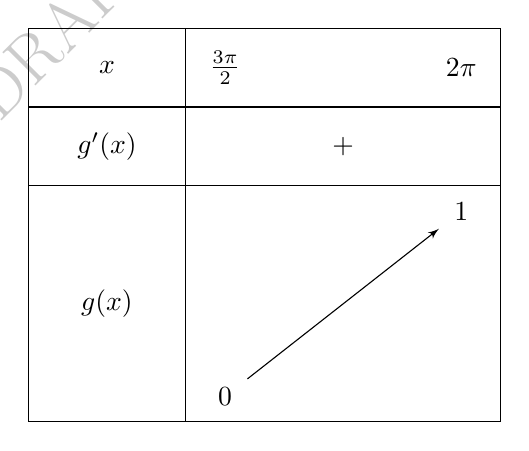
\begin{tikzpicture}
    % Initialisation du tableau
    \tkzTabInit[lgt=2, espcl=3]
    {$x$ /1, $g'(x)$ /1, $g(x)$ /3} 
    {$\frac{3\pi}{2}$, $2\pi$}

    % Ligne de signes de g'(x)
    \tkzTabLine{,+,}
    
    % Ligne de variations de g(x)
    \tkzTabVar{-/$0$, +/$1$,}
\end{tikzpicture}
\end{center}












\newpage
\quad

\quad

\textbf{{\LARGE Méthodologie : la dissertation de Culture Générale} }

\newpage

\section*{A. Principes}

 Une \textbf{dissertation} est la formalisation d'un raisonnement fondé sur la définition et la position d'un problème (Introduction) et aboutissant à la proposition d'une solution (B et/ou C de la troisième partie).

 Une dissertation doit mener un raisonnement progressif, construit, qui réponde 
à une problématique dégagée d'un sujet posé, presque toujours, sous la forme d'une 
citation ou d'une question. Elle comporte trois parties principales : une introduction; un plan progressif ( ou développement) généralement en trois parties, chacune composée de plusieurs sous-parties, des exemples bien développés et judicieux pour étayer le raisonnement; et une conclusion.
 
 
 \textbf{  L'évaluation privilégiera :}
 
\begin{itemize}
 \item la pertinence de l'analyse de la question dégagée à partir du sujet ;
 \item l'intérêt et la qualité de la réponse apportée à cette question initiale ;
\item la clarté de la démonstration, voire sa finesse, et sa progression ;
 \item la solidité de la culture littéraire du candidat(e) ;
 \item la justesse, la variété et la qualité de développement des exemples proposés pour illustrer la démonstration ;
 \item la qualité de l'expression (correction grammaticale et lexicale, orthographe).
\end{itemize}

\section*{B. Les différentes parties d'une dissertation}

Une dissertation comporte trois parties :

\quad
\textbf{ 1. L'introduction}

 Elle se fait en trois temps :

\quad

\textbf{a. Préambule ou présentation de l'œuvre}


Introduction du thème littéraire général dans lequel s'inscrit le sujet (la lecture, le roman, l'écriture, la poésie,etc.). Il s'agit d'entrer dans le devoir en justifiant le sujet/présentant le thème, le domaine auquel il se rattache.\\
Si vous trouvez rapidement une phrase d'ordre général (ou phrase dite d' $\ll$ accroche $\gg$) qui serve d"entrée en matière, c'est mieux. Mais ne perdez pas de temps à chercher une 
accroche séduisante, cela a peu d'importance. La phrase d'accroche peut concerner l'objet d'étude, le mouvement littéraire ou le thème.

Les phrases suivantes doivent présenter l'œuvre (ou les œuvres) avec sa 
date de parution, son auteur et le contexte littéraire
 
\textbf{ Il faut éviter de commencer par :}

$\circ$ Des platitudes trop générales, telles que $\ll$ depuis que l'homme est homme$\gg$, $\ll$ de tous temps $\gg$, $\ll$Depuis la nuit des temps$,\gg$ $\cdots$ ;

 $\circ$  Des remarques pleines de jargon qui veulent impressionner le correcteur ;

$\circ$ Des élucubrations inutiles sur la vie de l'auteur de la citation.\\ 



 
 
\textbf{\underline{ Attention :} Si vous commencez par une autre citation, il faut être prudent : elle 
doit être très $\ll$ accrocheuse $\gg$ mais ne doit pas créer de confusion avec celle qui est l'objet réel de la dissertation.}

\textbf{ b. Annonce du sujet}

 Présenter le sujet précis du devoir à l'intérieur de ce thème plus vaste (telle 
fonction de la lecture, telle définition du roman, telle conception de l'écriture 
ou de la poésie).

\begin{itemize}
\item Il s'agit de présenter le sujet en précisant le nom de l'auteur (ne dites de lui que ce qui est utile pour cerner et comprendre la citation) et époque : le recopier intégralement s'il est court ; s'il est assez long, le découper en segments que vous devez analyser tout en faisant apparaître les termes-clefs de la citation entre guillemets. Définir les termes-clefs afin d'amener la problématique que vous devez formuler (qui n'est pas la répétition du sujet sous une forme 
interrogative).
\item  Éviter les séries de questions directes.
\end{itemize}

\quad
\textbf{ c. Élaborer un problématique}

$-$ Lisez plusieurs fois la reformulation du sujet rédigée à partir de vos définitions. Au brouillon, écrivez toutes les idées qui vous viennent à l'esprit sur le sujet (exemples, autres, événements, ...).


$-$ Reformulez la question posée avec vos propres mots et montrez sa richesse et ses sous-entendus pour trouver la problématique qui est souvent un paradoxe qu'il faut dépasser.

$-$ La problématique est le fil directeur du devoir : votre plan doit répondre à la question qu'elle 
pose.

Comment les termes-clefs se relient-ils, s'articulent-ils entre eux ? Jouent-ils les uns par rapport aux autres de manière paradoxale, polémique ou problématique ? Où se 
situe la tension, la contradiction, le paradoxe, le problème ?
 
 Bien découper les propositions, les articulations, le jeu entre les termes dans des 
citations longues : penser à bien prendre en compte tous les termes et les liens logiques.


 Se poser diverses questions-clefs :
 
 \begin{itemize}
 \item Quels sont les enjeux exacts de ce sujet ?
 \item Quel est l'intérêt de la citation ?
 \item Quelles sont ses limites ?
 \item Qui parle et de quel point de vue ? Est-ce un auteur ? Un personnage littéraire ? Un critique ?
 
 Il s'agit de bien distinguer le thème (ce dont l'auteur parle) de la thèse (ce qu'il en dit).
 La problématique est-elle simple (question unique) ou complexe (entrelacs de 
plusieurs questions) ?
 
 Y a-t-il un contexte précis (historique, culturel, littéraire, idéologique $...$) à prendre en compte dans la citation ? Le nom de l'auteur, l'œuvre d'où est tirée la citation et sa date 
sont généralement donnés : en tirer parti (quel sens prend cette position par rapport à 
sa propre œuvre ?) sans non plus faire une dissertation d'histoire, d'histoire littéraire ni proposer une réflexion portant exclusivement sur l'auteur et son œuvre.
 
 Y a-t-il une légère distorsion entre la citation du sujet et la question qui l'accompagne, concernant le sujet lui-même ou le champ des exemples ?
 
 Y a-t-il un ton particulier (ironique, caricatural, polémique) qui sera à prendre en compte ?
\end{itemize}

\quad

\textbf{d.  Élaborer un plan}

Le plan d'une dissertation peut prendre diverses formes. L'important est qu'il répondre bien à votre problématique pour que vous évitez le hors-sujet.

\begin{itemize}
\item Utilisez votre brouillon initial sur lequel vous avez noté vos idées.
\item Classez ensuite ces idées par thématique ou argument.
\item Normalement, vous pourrez arrivez à deux ou trois idées principales, divisées en deux ou trois sous-parties qui seront illustrées par des exemples concrets.
\item N'oubliez pas de rédiger une transition entre chaque grande partie (conclusion de la partie actuelle et introduction de la partie suivante).
\end{itemize}

\vspace*{1.5cm}

\textbf{Les différents types de plan}

En dissertation, un plan bien structuré est essentiel pour la clarté et la cohérence de l'argumentation. Les types de plans peuvent varier en fonction du sujet, du style et de l'objectif de la dissertation.
 
On distingue \textbf{ quatre grands} types de plans : 
 
 $\rhd$ le \textbf{plan dialectique :} Ce type de plan est basé sur une opposition entre deux idées ou thèses et se développe en trois étapes : thèse (oui) – antithèse (non) – synthèse ou dépassement (mais). Ce plan peut correspondre aux sujets du type « Pensez-vous que... ? » / « Dans quelle mesure ? » ; 

\textbf{Exemple : La liberté d'expression est-elle absolue ?}

\begin{itemize}
\item \textbf{Thèse :} La liberté d'expression doit être absolue.
\item \textbf{ Antithèse :}La liberté d'expression doit être limitée.
\item \textbf{ Synthèse :}La liberté d'expression doit être encadrée par des lois pour protéger les individus et l'ordre public.\end{itemize}




$\rhd$ le \textbf{plan analytique :} Dans un plan analytique, le but est de diviser le sujet en plusieurs sous-parties logiques et d'examiner chaque aspect du problème. Il est souvent utilisé pour les sujets qui exigent une analyse détaillée de différents éléments ou phénomènes. Il se divise généralement en deux ou trois grandes parties, chaque partie étant une analyse détaillée d'un aspect particulier du sujet.
Il met en lumière les différents facteurs ou causes d'un problème, sans nécessairement chercher une opposition.

\textbf{Exemple :}  L'impact des réseaux sociaux sur la société

\textbf{I. L'impact positif des réseaux sociaux}

$-$ Facilitation de la communication et de l'information.

$-$ Renforcement des liens sociaux et communautaires.

\textbf{II. Les effets négatifs des réseaux sociaux
}

$-$ Isolement social et addiction.

$-$ Diffusion de fausses informations et manipulation.

\textbf{III. Les enjeux et régulations des réseaux sociaux}

$-$ Besoin de régulation des contenus.

$-$ Protection de la vie privée et des données personnelles.

\quad




$\rhd$ \textbf{ Le Plan Comparatif}

Ce plan consiste à comparer deux ou plusieurs éléments, idées ou phénomènes afin de dégager leurs différences ou similarités. Il est souvent utilisé dans des sujets où l'on doit confronter des théories, des événements, ou des situations.

\textbf{Exemple : }Comparer le système éducatif du Burkina Faso et celui d'un autre pays africain

\textbf{I. Le système éducatif au Burkina Faso}

$-$ Structure et caractéristiques du système.

\textbf{II. Le système éducatif d'un autre pays africain}

$-$ Comparaison des approches, structures et méthodes.

\textbf{III. Comparaison des résultats obtenus et des défis}

$-$ Analyse des points forts et faibles des deux systèmes.



$\rhd$ le \textbf{plan thématique :} il propose une réponse organisée autour des différents aspects d'un thème ou d'une notion. Vous pouvez poser ici les questions Quoi ? Comment ? Pourquoi ? qui vous aideront 
à circuler dans l'œuvre.

 \vspace*{1.5cm}
 
 En plus de ces plans, ils existent d'autres types de plans comme : \textbf{le plan problématique, le plan chronologie, le plan causes/conséquences, etc. }

\underline{\textbf{Élaborer un plan détaillé.}}
 
$\circ$ Noter au brouillon des citations ou des passages qui viendront illustrer les arguments. 

$\circ$ Dégager parmi toutes les remarques les grandes parties du plan qui ira du plus évident au 
plus complexe (deux ou trois). 

$\circ$ Pour chaque partie élaborer un sous plan : de deux à trois arguments ou sous-parties. Chaque 
argument devra s'appuyer sur au moins un exemple précis, auquel peuvent s'ajouter d'autres exemples plus ou moins développés. 

$\circ$ Rédiger au brouillon les transitions qui doivent à la fois conclure la partie et amener la partie suivante. 

\quad 
\textbf{\underline{ Remarque :} Qu'est-ce qu'un bon plan ?}
 
\quad Le plus difficile est bien évidemment de trouver un plan. Il ne faut pas viser la perfection qui n'existe pas. 

\quad Le bon plan est celui qui permet de développer une véritable réflexion à partir du sujet, de progresser dans une argumentation, de développer différentes remarques sans se répéter. L'autre écueil à éviter est le hors-sujet, n'hésitez pas à rappeler à chaque début les termes du sujet et à 
montrer en quoi chacune de vos parties y répond.


\quad
\quad
\textbf{2. Le développement}

Le développement d'une dissertation comporte toujours deux ou trois parties. Si vous faites une dissertation en deux parties, vous devez rédiger trois sous-parties pour chacune (deux si vous faites trois grandes parties).

Chaque partie soutient une idée centrale qui répond à la problématique, alors que chaque sous-parties s'articule autour d'un argument qui soutient et illustre l'idée directrice.

Vos arguments doivent absolument être illustrés par un exemple !

Entre chaque partie vous devez rédiger une transition qui conclut la partie précédente et annonce la partie suivante.


\textbf{3. La conclusion}

Elle comporte :
 
$\bullet$ Une réponse à la problématique grâce à un résumé du développement qui rappelle les grandes lignes de la démarche argumentative. 

$\bullet$ Une ouverture vers des éléments de réflexion en lien avec le sujet de dissertation. Il faut éviter à tout prix de reposer une nouvelle question.




\section*{C. Sujets types de dissertation}

\textbf{Sujet 1}

Dans \underline{Le degré zero de l'écriture}, Roland Barthes (1915-1980) écrit : $\ll$ \textbf{L'univers poétique est rempli de tourments qui font des poètes des gens qui n'ont jamais souri}$\gg$

Expliquez et discutez cette opinion dans un développement argumenté avec d'exemples tirés d'œuvres poétiques lues ou étudiées.

\quad

\textbf{Sujet 2}

Dans quelle mesure la montée du terrorisme au Burkina Faso (notamment l'action des groupes jihadistes comme le JNIM ou l'EIGS) est-elle liée aux failles de la gouvernance étatique et aux inégalités socio-économiques ?


\quad
\textbf{Sujet 3}

L'école n'est pas le seul moyen de réussir.

Discutez.

\quad

\textbf{Sujet 4}

$\ll$ La lutte contre le terrorisme  au Burkina Faso doit être envisagée en amont avec les forces armées de défenses et de sécurité, et en aval avec l'appui des populations$\gg$.

Justifiez ce point de vu avec 03 arguments et donnez trois limites.

\quad

\textbf{Sujet 5}

Le coup d'État de 2022 et la transition dirigée par le capitaine Ibrahim Traoré : rupture démocratique ou réponse nécessaire à l'effondrement sécuritaire ?

\quad

\textbf{Sujet 6}

D'après Albert Jacquart: $\ll$ Désormais la solidarité la plus nécessaire est celle de l'ensemble des habitants de la terre$\gg$.

Que vous inspire cette pensée?

\quad

\textbf{Sujet 7}

La liberté d'expression est-elle le baromètre de la démocratie?


\quad
\quad

\textbf{Sujet 8 :}

L'éducation au Burkina Faso peut-elle contribuer à l'amélioration des conditions sociales des jeunes ?


\quad
\quad

\textbf{Sujet 9 :} La démocratie est-elle réellement la forme de gouvernement la plus adaptée aux pays africains ?

\quad
\quad

\textbf{Sujet 10 :} L'accès à l'éducation pour tous au Burkina Faso : enjeux et défis.


\quad
\quad

\textbf{Sujet 11 :} L'éducation des jeunes filles au Burkina Faso : enjeux et perspectives.


\quad
\quad

\textbf{Sujet 12 :} Les réformes éducatives au Burkina Faso : quel impact sur la qualité de l'enseignement ?


\quad
\quad

\textbf{Sujet 13 :}
La fin de la présence militaire française et le rapprochement avec la Russie (groupe Wagner) : quels impacts sur la stabilité régionale et la lutte contre le terrorisme au Sahel ?

\quad
\quad

\textbf{Sujet 14 :}

Quel rôle jouent le chômage des jeunes et l'absence d'éducation dans la propagation des groupes armés au Burkina Faso ?

\quad
\quad

\textbf{Sujet 15 :}

La CEDEAO face à la crise burkinabè : entre sanctions politiques et impuissance face à la prolifération des coups d'État en Afrique de l'Ouest.




\quad
\quad

\textbf{Sujet 16 :}

L'orpaillage artisanal au Burkina Faso : enjeux économiques, tensions sociales et financement des groupes terroristes.


\quad



\textbf{Session 2016}

\textbf{\underline{Sujet :}}Faisant l'écho à l'avènement de la société de l'information, Gaston MIALARET (in Pédagogie générale, 1991, p.530) affirme :$\ll$ avant on savait tout sur le village mais rien sur le monde; aujourd'hui on sait tout sur le monde mais rien sur le village $\gg$.

Justifiez cette réflexion de MIALARET, Présentez deux(02) conséquences possibles de cette situation et avancez deux(02) mesures que l'on pourrait mettre en œuvre pou essayer de trouver un équilibre.


\quad
\textbf{\underline{Session 2017}}

$\ll$ c'est dans l'effort et non dans la réussite qu'on puise la satisfaction. Le plein effort, c'est la pleine victoire. Un effort continuel vers la perfection est le devoir de tout homme et porte en lui sa récompense $\gg$.

Expliquez et discutez cette pensée de Gandhi.


\quad
\textbf{\underline{Session 2021 (mesure nouvelle}}

\textbf{\underline{Sujet :} Pour l'accès et le maintien des filles à l'école, il n'appartient pas seulement à ces dernières de s'adapter aux exigences de la vie scolaire, mais aussi à l'institution scolaire de prendre en charge leurs besoins spécifiques.}

\quad Sous la forme d'une dissertation, développez dans une première partie, trois arguments qui traduisent les obstacles à la scolarisation des filles du Burkina Faso, et proposer dans une seconde partie, trois (03) solutions à même d'améliorer leur accès et leur maintien scolaires.


\quad
\textbf{\underline{Session 2021}}

\textbf{\underline{Sujet :}} \quad La jeunesse, fondement essentiel de l'avenir des sociétés, est responsable de son action comme de son inaction. Le monde dont elle est l'héritière lui exigera des comptes plus tard.

\quad Dans une argumentation bien structurée, justifiez cette assertion et dites en quoi l'éducation peut permettre à la jeunesse de faire le bon choix.

\quad Chaque partie comportera deux arguments illustrés d'exemples précis.


\quad
\quad




\section*{\textbf{E. PROPOSITIONS DE CORRECTIONS DES SUJETS DE CULTURE GÉNÉRALE}}

\textbf{Correction de session 2017}


\textbf{Introduction}

Dans une société où la réussite est souvent perçue comme le seul critère de valorisation, il est facile d'oublier que l'effort en lui-même constitue une richesse. Gandhi, dans cette pensée, invite à repenser notre relation à l'effort et au succès : il affirme que la satisfaction réside moins dans l'atteinte des objectifs que dans la sincérité et l'intensité de l'engagement. Il nous rappelle également que l'effort constant en quête de perfection est une obligation morale qui porte en elle sa propre récompense. Cette réflexion soulève des interrogations fondamentales : pourquoi l'effort aurait-il plus de valeur que le résultat ? En quoi cette quête d'amélioration continue constitue-t-elle une victoire personnelle et universelle ? Après avoir clarifié cette pensée, nous discuterons de sa pertinence et de ses limites dans le contexte contemporain.


\textbf{Développement}

\textbf{I. La valeur intrinsèque de l'effort}

Gandhi souligne que l'effort, en tant qu'acte volontaire et sincère, porte en lui-même une satisfaction profonde. Cette idée repose sur le fait que l'effort est une manifestation de notre volonté de progresser et de nous améliorer, indépendamment des résultats obtenus.  

\textbf{1. Une source de satisfaction personnelle} 
 
   L'effort déployé dans un travail ou une activité procure une forme d'accomplissement. Il renforce la confiance en soi et donne un sens à nos actions, même lorsque le succès n'est pas garanti. Par exemple, un étudiant qui se consacre avec sérieux à ses études tire une fierté de son engagement, quelle que soit l'issue de ses examens.  
   
\textbf{2. Une éthique universelle 
   }
   
   Dans de nombreuses cultures et traditions, l'effort est perçu comme une vertu morale. Les philosophies stoïcienne ou bouddhiste, par exemple, prônent l'idée que l'essentiel est dans la maîtrise de soi et dans le travail sur ses imperfections, plutôt que dans la recherche de récompenses extérieures.

\textbf{II. L'effort comme une victoire en soi}

Gandhi affirme que le plein effort équivaut à une victoire. Cette vision valorise la démarche plus que le résultat, et encourage un dépassement de soi constant.  
\textbf{1. Le dépassement personnel
}
   Faire de son mieux, quel que soit le domaine, permet de repousser ses limites et de progresser. Ce processus renforce le caractère et l'endurance. Par exemple, un athlète qui s'entraîne sans relâche pour une compétition peut considérer son engagement comme une victoire, même s'il ne gagne pas la médaille d'or. 
    
\textbf{2. Une victoire intérieure}
   La satisfaction tirée de l'effort sincère va au-delà des jugements externes. Elle permet de vivre en accord avec ses valeurs, ce qui constitue une forme de victoire personnelle. Gandhi, dans sa propre vie, a illustré cette idée en luttant pour l'indépendance de l'Inde avec des moyens non violents, malgré les immenses défis auxquels il était confronté.

\textbf{III. Les limites et les enjeux contemporains de cette pensée}

Si la philosophie de Gandhi est inspirante, elle peut sembler difficilement applicable dans certains contextes modernes.
 
\textbf{1. L'importance des résultats dans la société actuelle}
  
   Dans un monde orienté vers la performance et les résultats mesurables, il est parfois difficile de valoriser uniquement l'effort. Par exemple, dans un cadre professionnel, un travailleur pourrait déployer beaucoup d'efforts, mais ne pas être reconnu s'il n'atteint pas les objectifs fixés. 
    
\textbf{2. Le risque de l'épuisement  }

   Exiger un effort constant sans se soucier des résultats peut aussi conduire à une pression excessive et à un épuisement moral ou physique. Il est donc nécessaire de trouver un équilibre entre persévérance et repos, entre quête de perfection et acceptation de ses limites.  

\textbf{IV. L'effort comme chemin vers une perfection morale}

Enfin, Gandhi élève l'effort au rang de devoir universel. Selon lui, chercher continuellement à s'améliorer est un moyen de se réaliser pleinement et de contribuer au bien commun.
  
\textbf{1. Un devoir moral } 
   L'effort constant incarne une quête de perfection morale et d'éthique. En travaillant sur soi-même, on devient plus apte à servir les autres et à avoir un impact positif sur la société.  
   
\textbf{2. La récompense intérieure  }

   Cet effort ne dépend pas de l'approbation des autres ni de la reconnaissance extérieure, mais de la satisfaction personnelle et du sentiment d'avoir fait ce qui est juste. Cela est particulièrement pertinent dans un monde où la recherche de validation extérieure peut devenir oppressante.


\textbf{Transition vers la conclusion}

Ainsi, la pensée de Gandhi nous invite à repenser notre rapport à l'effort, à voir dans le cheminement un enrichissement personnel et une victoire en soi. Pourtant, cette vision idéale nécessite d'être nuancée pour rester applicable aux réalités contemporaines, où effort et résultats doivent souvent être conciliés. 



\quad

\quad

\textbf{Conclusion}

La pensée de Gandhi nous enseigne que l'essence de la satisfaction et de la victoire réside dans l'effort sincère et constant plutôt que dans la simple quête de résultats. Elle valorise une vision humaniste où l'amélioration personnelle et le dépassement de soi priment sur la réussite matérielle ou sociale. Cette approche, bien qu'exigeante, nous invite à trouver un sens profond dans nos actions quotidiennes et à embrasser l'idée que la perfection n'est pas un objectif fixe, mais un cheminement continu. Cependant, dans un monde où les résultats concrets sont souvent indispensables, il est nécessaire de trouver un équilibre entre cette philosophie idéale et les réalités pragmatiques de la vie moderne. Gandhi nous propose ainsi une leçon intemporelle : c'est dans la sincérité de nos efforts que réside notre véritable accomplissement.

\quad
\quad

\textbf{Correction de 2021}

\textbf{Introduction}

La jeunesse est souvent qualifiée de $\ll$force  vive$\gg$ d'une société, représentant son potentiel de transformation et d'innovation. Cependant, en tant que l'héritière du monde actuel, elle porte une responsabilité immense, car ses actions ou son inaction auront des répercussions profondes sur l'avenir. Face à cette réalité, l'éducation joue un rôle fondamental pour guider la jeunesse dans la prise de décisions éclairées. Nous examinerons d'abord pourquoi la jeunesse est responsable de ses choix, avant de montrer comment l'éducation peut l'aider à assumer cette responsabilité.


\textbf{Développement}

Première partie : La jeunesse est responsable de son action comme de son inaction

1. L'action de la jeunesse façonne l'avenir d'une société
  
Les jeunes, par leurs idées et leurs initiatives, influencent directement l'évolution des communautés. Par exemple, Malala Yousafzai, militante pour l'éducation des filles, a démontré qu'une jeune personne peut transformer les mentalités et influencer des politiques mondiales. Une jeunesse engagée dans des actions positives contribue à la construction d'un monde meilleur.

2. L'inaction a des conséquences graves  

À l'inverse, l'inaction des jeunes face à des enjeux majeurs, comme le changement climatique, peut aggraver les crises existantes. Par exemple, si les jeunes restent passifs face à la déforestation en Afrique, les écosystèmes se dégradent, ce qui compromet leur propre avenir. Leur silence ou leur indifférence est une forme de responsabilité qui les rattrapera.

Deuxième partie : Le rôle de l'éducation pour orienter la jeunesse vers le bon choix

1. L'éducation donne les outils pour comprendre les enjeux.
  
Une éducation de qualité permet aux jeunes d'acquérir les compétences nécessaires pour analyser les défis contemporains. Par exemple, dans les écoles qui intègrent l'éducation environnementale, les élèves deviennent souvent des militants actifs pour des causes écologiques. L'éducation leur ouvre ainsi les yeux sur les problématiques complexes de leur époque.

2. L'éducation développe un sens des responsabilités et des valeurs.
  
Au-delà des connaissances, l'éducation forme les individus à des valeurs comme l'éthique, la solidarité et la citoyenneté. Par exemple, les programmes qui mettent l'accent sur le volontariat, comme les "services civiques", incitent les jeunes à s'impliquer dans leur communauté. Une jeunesse éduquée est donc mieux préparée à faire des choix responsables et durables.

\textbf{Conclusion}

En somme, la jeunesse porte la responsabilité de l'avenir à travers ses actions et ses choix. Si elle s'implique activement, elle peut bâtir un monde meilleur, mais son inaction pourrait avoir des conséquences désastreuses. L'éducation apparaît ainsi comme un levier indispensable pour éclairer cette jeunesse et la préparer à prendre des décisions éclairées, guidées par des valeurs et une vision claire des enjeux mondiaux. Dès lors, investir dans l'éducation, c'est investir dans un avenir prometteur.


\quad
\quad
\textbf{Correction du sujet 1}

\textbf{ Introduction}

\textbf{ Accroche :} La poésie est souvent perçue comme un genre littéraire qui plonge au cœur des émotions humaines, explorant des thèmes profonds comme la douleur, la mélancolie, ou les tourments de l'âme.

\textbf{ Présentation de la citation :} \emph{Roland Barthes}, dans Le degré zéro de l'écriture, affirme que l'univers poétique est habité par des tourments, suggérant que les poètes sont marqués par une profonde gravité, incapables de sourire.

\textbf{ Problématique :} Cette vision des poètes comme figures tourmentées est-elle représentative de l'ensemble de l'univers poétique ? Existe-t-il des contre-exemples ou des nuances à apporter à cette idée ?

\textbf{ Annonce du plan :} Nous examinerons tout d'abord les œuvres qui confirment cette opinion, avant d'explorer les exceptions et de conclure sur la diversité de l'univers poétique.

\quad
I. L'univers poétique comme miroir des tourments humains
Barthes semble mettre en avant la capacité de la poésie à exprimer les souffrances et les tourments, qui sont des thèmes récurrents dans l'histoire littéraire.

1. Les poètes maudits : une figure emblématique de la souffrance poétique

Exemple : Charles Baudelaire (Les Fleurs du mal)
Baudelaire explore des thèmes comme le spleen, l'ennui, et la déchéance. Ses poèmes, tels que L'Albatros ou Spleen, mettent en scène un univers sombre où le poète est en proie à une souffrance existentielle.
Paul Verlaine et les tourments de l'amour (Romances sans paroles, Sagesse).
Son écriture reflète des conflits intérieurs liés à l'amour, la culpabilité, et la recherche spirituelle.

2. La poésie comme exutoire des douleurs personnelles

Exemple : Arthur Rimbaud (Une Saison en enfer).
Rimbaud exprime sa révolte contre le monde et ses propres blessures intérieures.
Anna Akhmatova : Dans sa poésie, la douleur liée à la guerre et à la répression soviétique imprègne ses œuvres, notamment dans Requiem.

\quad
II. Une vision partielle : la poésie peut aussi célébrer la joie et l'émerveillement
Bien que Barthes souligne les tourments des poètes, il existe des œuvres poétiques qui explorent des thèmes légers, joyeux ou empreints d'émerveillement.

1. La célébration de la beauté et de la nature

Exemple : Alphonse de Lamartine (Le Lac).
Bien que teinté de mélancolie, ce poème célèbre également la beauté de la nature et l'immortalité des souvenirs.
Victor Hugo (Les Contemplations).
Certains poèmes de Hugo, comme Demain, dès l'aube, mêlent douleur et espoir, montrant que l'écriture poétique n'est pas uniquement marquée par la souffrance.

2. L'humour et l'ironie dans la poésie

Exemple : Jacques Prévert (Paroles).
Prévert écrit des poèmes pleins d'ironie et de légèreté, jouant avec les mots et les images pour offrir un regard critique mais amusé sur la société.
Francis Ponge : Dans Le Parti pris des choses, Ponge célèbre des objets simples de la vie quotidienne avec une poésie décalée et ludique.

\quad
III. Vers une vision nuancée de la condition du poète
La citation de Barthes peut être interprétée comme une généralisation. Cependant, l'univers poétique est divers et reflète une gamme complète d'émotions humaines.

1. La poésie comme catharsis : une nécessité d'exprimer les tourments
Même lorsque la poésie aborde des thèmes sombres, elle permet au poète de se libérer de ses souffrances. Cela peut être vu comme une forme de sourire intérieur, une réconciliation avec soi-même.

2. La poésie moderne : un espace d'exploration ludique et expérimental
Dans la poésie contemporaine, de nombreux poètes, comme Raymond Queneau (Cent Mille Milliards de Poèmes), utilisent l'écriture poétique pour expérimenter et jouer avec la langue, rompant avec l'image traditionnelle du poète tourmenté.

\quad
\quad
\textbf{ Conclusion}
\textbf{Résumé : }L'affirmation de Barthes souligne à juste titre la prévalence des thèmes sombres et tourmentés dans l'univers poétique, comme en témoignent des œuvres de Baudelaire, Verlaine ou Rimbaud. Cependant, cette vision n'englobe pas toute la richesse de la poésie, qui peut aussi célébrer la joie, l'émerveillement, et l'humour.

\textbf{Ouverture :} La poésie, par sa diversité, reflète toute la complexité de la condition humaine. Peut-être que l'univers poétique n'est pas tant un lieu de souffrance qu'un espace où les émotions humaines, qu'elles soient sombres ou lumineuses, trouvent une expression universelle.




\quad

\textbf{Correction sujet 2}

\textbf{Introduction}

\textbf{Contexte général :} Le Burkina Faso est confronté depuis 2015 à une montée inquiétante du terrorisme, marqué par les actions de groupes jihadistes comme le JNIM (Jama’at Nusrat al-Islam wal-Muslimin) et l’EIGS (État Islamique dans le Grand Sahara). Ces attaques ont plongé le pays dans une crise sécuritaire sans précédent.

\textbf{Problématique :} Cette montée du terrorisme peut-elle être expliquée en partie par les failles de la gouvernance étatique et les inégalités socio-économiques ? Ces facteurs internes aggravent-ils la vulnérabilité du pays face à ces menaces ?

\textbf{Annonce du plan :} Nous examinerons d'abord les failles de la gouvernance qui ont favorisé l'émergence de groupes terroristes, avant d'analyser les inégalités socio-économiques comme facteurs sous-jacents. Enfin, nous proposerons une réflexion sur les solutions possibles.

\quad
\quad


I. Les failles de la gouvernance étatique : une porte ouverte au terrorisme
La faiblesse de l'État burkinabè a favorisé l'implantation des groupes jihadistes.

1. Un déficit de présence étatique dans les zones rurales
Faible contrôle territorial : De nombreuses zones périphériques, notamment au Sahel, ont historiquement souffert d'un manque d'infrastructures, de services publics (santé, éducation) et de sécurité. Cela a laissé un vide que les groupes terroristes ont exploité.

Exemple : Les régions du Sahel et de l'Est du Burkina, où l'État est souvent absent, sont devenues des bastions pour le JNIM et l'EIGS.

2. Corruption et inefficacité administrative
La corruption dans les institutions publiques a affaibli la confiance des populations envers l'État, rendant les communautés plus sensibles aux discours anti-gouvernementaux des jihadistes.

Exemple : Le détournement de fonds destinés aux projets de développement ou à la lutte contre le terrorisme.

3. Crise de légitimité politique
Les transitions politiques chaotiques et le manque de dialogue inclusif ont exacerbé les frustrations sociales. Les groupes jihadistes exploitent ces divisions pour recruter.
Exemple : Les tensions après la chute de Blaise Compaoré en 2014 ont créé une période d'instabilité propice à l'émergence de nouvelles menaces.

\quad
II. Les inégalités socio-économiques : un terreau fertile pour le terrorisme
Les inégalités, exacerbées par la pauvreté et l'exclusion sociale, ont alimenté les frustrations et les tensions communautaires.

1. Pauvreté et chômage des jeunes.

Le Burkina Faso est l'un des pays les plus pauvres du monde, avec un taux élevé de chômage, notamment chez les jeunes. Ces derniers sont particulièrement vulnérables au recrutement par les groupes jihadistes, qui leur offrent un revenu et un sentiment d'appartenance.

Exemple : Les promesses financières des jihadistes pour des jeunes marginalisés dans les zones rurales.

2. Inégalités régionales
Certaines régions (comme le Sahel) sont historiquement marginalisées par rapport à d'autres (comme la région du Centre). Cela crée un sentiment d'injustice qui peut être exploité par les groupes jihadistes.

Exemple : L'absence d'écoles ou de centres de santé dans les zones rurales.

3. Tensions communautaires et ethniques

Les jihadistes instrumentalisent souvent les tensions entre communautés (ex. : agriculteurs contre éleveurs) pour semer la division et renforcer leur emprise.

Exemple : L’EIGS exploite les tensions entre Peuls et autres communautés pour recruter et justifier ses actions.

\quad

III. Vers une réponse globale : réduire les vulnérabilités internes.
Pour contrer la montée du terrorisme, il est crucial de traiter les causes profondes liées à la gouvernance et aux inégalités.

1. Renforcement de la gouvernance locale

Améliorer la présence de l’État dans les zones reculées à travers des investissements dans les infrastructures et les services publics.
Promouvoir une gouvernance participative pour renforcer la confiance entre l’État et les populations locales.

2. Lutte contre les inégalités socio-économiques
Développer des programmes de création d'emplois pour les jeunes, notamment dans les zones rurales.
Réduire les disparités régionales en investissant davantage dans les régions marginalisées.

3. Réconciliation nationale et dialogue intercommunautaire
Favoriser le dialogue entre communautés pour apaiser les tensions ethniques et promouvoir la cohésion sociale.
S'appuyer sur les chefs traditionnels et religieux pour promouvoir la paix.

4. Renforcer la coopération sécuritaire
Collaborer avec les pays voisins pour démanteler les réseaux jihadistes transfrontaliers.
Moderniser les forces de sécurité et renforcer les capacités de renseignement.

\quad

\textbf{ Conclusion}

\textbf{ Résumé :} La montée du terrorisme au Burkina Faso est indissociable des failles de la gouvernance et des inégalités socio-économiques. Ces facteurs ont créé un terreau favorable pour l'implantation et l'expansion des groupes jihadistes comme le JNIM et l’EIGS.


\textbf{Ouverture :} La réponse au terrorisme ne peut être uniquement militaire. Elle doit s'accompagner de réformes structurelles profondes pour traiter les causes sous-jacentes de la crise et construire un avenir de stabilité et de paix durable au Burkina Faso.


\quad

\textbf{Correction du sujet 3}

\textbf{ Introduction}

\textbf{Contexte(préambule) :} L'école est souvent perçue comme le chemin principal vers le succès, en offrant des compétences, des diplômes et des opportunités d'emploi. Cependant, de nombreuses réussites dans la vie ont montré que l'école n'est pas le seul moyen d'atteindre ses objectifs.

\textbf{ Problématique :} Dans quelle mesure l'école est-elle indispensable pour réussir ? Existe-t-il d'autres voies permettant d'accomplir ses ambitions et d'obtenir une reconnaissance sociale ou personnelle ?

\textbf{ Annonce du plan :} Nous discuterons tout d'abord de l'importance de l'école dans la réussite, puis des limites de cette institution, avant d'explorer d'autres moyens de réussir dans la vie.

\quad
I. L'école : un moyen structuré et efficace pour réussir
L'école reste un pilier fondamental pour construire une base solide en vue du succès.

1. Accès aux connaissances et aux compétences
L'école fournit des connaissances théoriques et pratiques indispensables dans de nombreux domaines professionnels.

Exemple : Des métiers comme médecin, ingénieur ou avocat nécessitent des diplômes spécifiques.

2. Reconnaissance sociale
Le système scolaire attribue des diplômes qui sont des critères de validation universels dans le monde du travail.

Exemple : Un employeur privilégiera souvent un candidat ayant un diplôme pertinent.

3. Développement personnel et social
L'école permet de développer des compétences comme la discipline, la collaboration, et la pensée critique.

Exemple : Les activités parascolaires (clubs, compétitions) renforcent les aptitudes interpersonnelles.

\quad
II. Les limites de l'école comme unique moyen de réussite
Malgré ses avantages, l'école ne garantit pas toujours le succès et peut ne pas convenir à tout le monde.

1. L'école ne développe pas toujours les talents individuels.

Le système scolaire, souvent standardisé, peut négliger les talents et intérêts spécifiques des individus.

Exemple : De nombreux artistes, sportifs ou entrepreneurs brillants ont échoué à l'école parce que leur potentiel n'y était pas valorisé.

2. Inadéquation avec le marché du travail

Les diplômes scolaires ne garantissent pas toujours un emploi, en particulier dans des contextes où le chômage est élevé.

Exemple : Un diplômé sans expérience pratique peut avoir des difficultés à trouver un emploi adapté.

3. L'école ne prend pas en compte l'intelligence pratique
Certaines formes d'intelligence, comme l'intelligence émotionnelle, sociale ou manuelle, ne sont pas suffisamment valorisées dans le système scolaire.

Exemple : Les artisans ou commerçants réussissent souvent sans avoir fait d'études supérieures.

\quad
III. D'autres moyens de réussir dans la vie
Le succès peut être atteint par d'autres voies, notamment grâce à la persévérance, la créativité et l'adaptabilité.

1. L'apprentissage informel et autodidacte

L'ère numérique offre une multitude de ressources éducatives gratuites ou accessibles, permettant d'apprendre sans passer par l'école traditionnelle.

Exemple : Bill Gates, autodidacte dans l'informatique, a quitté l'université mais a fondé Microsoft.

2. Les métiers manuels et techniques

Des métiers comme maçon, couturier ou mécanicien ne nécessitent pas de longues études mais peuvent mener à un succès économique et personnel.

Exemple : De nombreux entrepreneurs locaux ont bâti des entreprises prospères en s'appuyant sur leurs compétences pratiques.

3. La créativité et l'innovation

Les secteurs artistiques (musique, cinéma, mode) montrent que des individus peuvent réussir grâce à leur talent et leur originalité, sans passer par un cursus scolaire classique.

Exemple : Des artistes comme Bob Marley ou des créateurs comme Coco Chanel n'ont pas suivi de formation académique rigoureuse.

4. Les réseaux sociaux et le marketing personnel
À l'ère d'Internet, les plateformes numériques permettent à des individus de se faire connaître et de réussir, indépendamment de leur parcours scolaire.

Exemple : Les influenceurs et entrepreneurs numériques qui bâtissent leur carrière sur des compétences pratiques et du marketing personnel.

\textbf{ Conclusion}

\textbf{ Synthèse }: L'école constitue un moyen structuré et efficace de réussir, mais elle n'est pas le seul chemin. Le succès peut également être atteint par des voies alternatives, comme l'apprentissage autodidacte, les métiers techniques ou la créativité.

\textbf{Réflexion personnelle :} L'essentiel pour réussir réside dans la capacité à identifier ses talents, à persévérer face aux obstacles et à s'adapter à un monde en constante évolution.

\textbf{ Ouverture :} Plutôt que d'opposer école et autres moyens de réussite, il serait pertinent de concevoir un système éducatif plus inclusif et flexible, capable de valoriser les divers talents et aspirations des individus.






\quad

\textbf{Correction du sujet 4}


\textbf{ Introduction}

Le terrorisme au Burkina Faso, marqué par les actions de groupes comme le JNIM et l’EIGS, représente une menace croissante pour la sécurité et la stabilité du pays. La lutte contre ce fléau ne peut se limiter à des opérations militaires, elle doit également mobiliser les populations civiles pour garantir une réponse efficace. Cette approche, combinant les efforts des Forces Armées de Défense et de Sécurité (FDS) et la collaboration des populations, repose sur une logique d'intervention globale. Cependant, cette stratégie présente aussi des limites qu'il convient d'examiner.

Arguments en faveur de cette approche

1. La complémentarité des forces armées et des populations

Les FDS disposent des moyens techniques et stratégiques pour contrer les groupes armés, mais leur efficacité dépend aussi du renseignement fourni par les populations locales.

Exemple : Les communautés vivant dans des zones reculées peuvent signaler les mouvements suspects ou les caches d'armes des terroristes.

Justification : Cela améliore les capacités d'intervention des FDS en réduisant le facteur surprise des attaques ennemies.

2. La légitimité renforcée par l'implication des populations
Associer les populations aux efforts de lutte contre le terrorisme renforce la légitimité des actions des FDS.

Exemple : Des comités locaux de vigilance peuvent être créés pour surveiller les zones à risque, favorisant un sentiment de responsabilité collective.
Justification : Une collaboration étroite diminue les tensions entre civils et militaires, renforçant la confiance mutuelle et l'engagement communautaire.

3. Une meilleure résilience face à la radicalisation
L'appui des populations permet d'identifier et de contrer les discours de radicalisation propagés par les groupes terroristes.

Exemple : Des leaders communautaires ou religieux peuvent sensibiliser les jeunes contre les idéologies extrémistes.

Justification : Cela limite le recrutement des terroristes parmi les populations vulnérables, affaiblissant leur base sociale.

Les limites de cette approche

1. La méfiance entre populations et forces de défense
Dans certaines régions, les populations perçoivent les FDS comme une force oppressive, ce qui entrave leur coopération.

Exemple : Des accusations d'exactions ou d'abus par certains membres des FDS peuvent dissuader les civils de fournir des informations utiles.

2. Le manque de moyens pour les FDS et les populations
La lutte contre le terrorisme nécessite des moyens logistiques, financiers et humains souvent insuffisants dans un pays en développement comme le Burkina Faso.

Exemple : Les comités de vigilance locaux manquent souvent d'équipements adéquats pour se défendre face à des groupes armés bien organisés.
3. Les risques
 d'instrumentalisation des populations
 
L'implication des populations dans la lutte contre le terrorisme peut les exposer à des représailles de la part des groupes armés.

Exemple : Les terroristes peuvent cibler des villages ayant collaboré avec les FDS, aggravant la situation sécuritaire pour les civils.

\quad

\textbf{ Conclusion}

La lutte contre le terrorisme au Burkina Faso doit effectivement combiner les efforts des FDS et l'appui des populations. Cette approche favorise une meilleure efficacité, une légitimité accrue et une résilience face à la radicalisation. Cependant, elle reste limitée par les problèmes de méfiance, le manque de moyens et les risques pour les populations. Une solution durable résiderait dans une réforme des institutions, un renforcement des capacités des FDS et une meilleure protection des communautés civiles impliquées dans la lutte contre le terrorisme.



\quad
\quad

\textbf{Correction du sujet 5}

\textbf{Introduction}

Le coup d'État de 2022 au Burkina Faso, qui a vu le capitaine Ibrahim Traoré accéder au pouvoir, a suscité des débats intenses sur sa nature et ses implications. Certains y voient une rupture avec les principes démocratiques établis, tandis que d'autres le perçoivent comme une réponse pragmatique à une situation sécuritaire et socio-politique critique. Cette analyse vise à examiner les deux perspectives pour mieux comprendre les enjeux de cet événement majeur.

1. Le coup d'État : une rupture démocratique

1.1. L'interruption du processus démocratique

Le renversement du pouvoir civil issu d'élections démocratiques constitue une violation des normes constitutionnelles.

Exemple : Le président Roch Marc Christian Kaboré, bien que critiqué pour son incapacité à gérer l'insécurité, avait été élu par le peuple dans un cadre démocratique.
Analyse : Ce coup d'État fragilise davantage les institutions démocratiques dans un pays où la gouvernance civile reste fragile.

1.2. Un recul pour la stabilité institutionnelle

Les transitions militaires entraînent souvent une instabilité politique et institutionnelle.

Exemple : Depuis 2015, le Burkina Faso a connu plusieurs changements de régime non démocratiques, sapant la confiance des citoyens envers leurs institutions.
Analyse : Cette instabilité complique la mise en place de réformes durables nécessaires à la bonne gouvernance.

1.3. Les risques de légitimité à l'international

Les partenaires internationaux, souvent attachés aux principes démocratiques, ont vu ce coup comme une rupture inacceptable.

Exemple : La suspension du Burkina Faso par certaines organisations comme la CEDEAO montre que ce coup d'État a terni l'image du pays sur la scène internationale.

Analyse : Cette situation peut limiter l'accès à des financements et à une coopération cruciale pour la lutte contre l'insécurité.

2. Le coup d'État : une réponse nécessaire à l'effondrement sécuritaire

2.1. Une incapacité criante de l'ancien régime à gérer l'insécurité
Avant le coup d'État, le Burkina Faso faisait face à une crise sécuritaire grandissante, marquée par des attaques terroristes incessantes et l'effondrement des services publics.

Exemple : En 2022, près de 40/100 du territoire était hors du contrôle de l'État, avec des millions de déplacés internes.

Analyse : Le capitaine Ibrahim Traoré a justifié son action comme une nécessité pour sauver le pays d'un effondrement total.

2.2. Un renforcement immédiat des efforts militaires

La transition dirigée par Traoré a mis un accent particulier sur le redéploiement des forces armées et l'implication des volontaires pour la défense de la patrie (VDP).

Exemple : Sous sa direction, plusieurs initiatives ont été lancées pour regagner les zones occupées par les groupes terroristes.

Analyse : Cette approche a rassuré une partie de la population qui se sentait abandonnée sous le régime précédent.

2.3. Une réponse populaire et nationale.

L'arrivée d’Ibrahim Traoré au pouvoir a été perçue par de nombreux Burkinabè comme un acte patriotique.

Exemple : Les manifestations de soutien dans plusieurs régions montrent que ce coup d'État a bénéficié d'une certaine adhésion populaire.

Analyse : Le sentiment d'urgence sécuritaire semble avoir primé sur les principes démocratiques pour une grande partie de la population.

3. Les dilemmes entre rupture démocratique et réponse nécessaire

3.1. La tension entre urgence et légitimité

Bien que justifié par l'urgence sécuritaire, le coup d'État soulève des questions sur la durabilité de solutions imposées par la force.

Exemple : Si la sécurité s'améliore sous Traoré, il faudra tout de même préparer un retour à un ordre constitutionnel pour éviter un cycle de coups d'État.

3.2. La nécessaire réconciliation entre démocratie et sécurité
La gestion de la transition doit concilier les impératifs sécuritaires avec un plan clair pour rétablir la démocratie.

Exemple : Les promesses d'organiser des élections d'ici 2025 seront un test pour évaluer la volonté de la transition à restaurer l'ordre démocratique.

 \textbf{Conclusion}
 
Le coup d'État de 2022 au Burkina Faso dirigé par le capitaine Ibrahim Traoré peut être perçu à la fois comme une rupture démocratique et une réponse nécessaire à l'effondrement sécuritaire. Si la transition a permis de redonner un souffle nouveau dans la lutte contre le terrorisme, elle soulève des interrogations sur l'avenir politique du pays. La clé réside dans la capacité du régime à équilibrer les exigences sécuritaires et la restauration de l'ordre démocratique, en évitant une dépendance excessive à des solutions militaires.



\quad
\quad
\textbf{Correction du sujet 6}

\textbf{Introduction}

Albert Jacquard, biologiste et humaniste, met en avant une vision globale et universelle de la solidarité. Cette citation, "Désormais la solidarité la plus nécessaire est celle de l'ensemble des habitants de la terre", insiste sur l'importance de l'interdépendance entre les êtres humains dans un monde de plus en plus globalisé. Dans un contexte marqué par des crises multiples — environnementales, économiques, sanitaires, et sociales — cette affirmation nous invite à réfléchir à l'urgence d'une solidarité mondiale. Nous analyserons cette idée à travers trois axes : la nécessité d'une solidarité universelle, les défis à surmonter pour l'atteindre, et les limites éventuelles de cette perspective.

1. La nécessité d'une solidarité universelle

1.1. L'interconnexion des défis mondiaux
Les crises modernes, telles que le réchauffement climatique, les pandémies (comme le COVID-19), et les inégalités sociales, affectent tous les habitants de la planète sans distinction de frontières.

Exemple : Le changement climatique, responsable de catastrophes naturelles croissantes, exige une action collective. Les pays pollueurs doivent réduire leurs émissions pour éviter des conséquences désastreuses pour toute l'humanité.

Analyse : Ces enjeux ne peuvent être résolus qu'avec une solidarité globale, car ils dépassent les capacités individuelles des nations.

1.2. Une humanité interdépendante
Les progrès technologiques et économiques ont intensifié l'interdépendance entre les peuples.

Exemple : La chaîne d'approvisionnement mondiale illustre que le bien-être d'un pays dépend de la stabilité des autres. Une crise en Asie peut rapidement affecter l'Europe ou l'Afrique.

Analyse : La solidarité n'est plus une option morale, mais une nécessité fonctionnelle pour maintenir un équilibre global.

1.3. Un impératif éthique
La solidarité mondiale repose aussi sur une reconnaissance de l'humanité partagée.

Exemple : La Déclaration universelle des droits de l'homme affirme que tous les humains ont droit à une vie digne.

Analyse : L'idéal de solidarité repose sur la conviction que nous sommes coresponsables du bien-être collectif.

2. Les défis de la solidarité mondiale

2.1. Les inégalités entre les nations
Les écarts économiques et sociaux entre les pays riches et pauvres rendent la solidarité difficile à mettre en œuvre.

Exemple : Lors de la pandémie de COVID-19, les pays riches ont monopolisé les vaccins, privant les pays pauvres d'un accès équitable.

Analyse : Tant que les intérêts économiques domineront, la solidarité mondiale restera inégale et insuffisante.

2.2. Les conflits d'intérêts nationaux
Chaque pays tend à privilégier ses propres intérêts, même au détriment du bien commun.

Exemple : Les accords climatiques, comme celui de Paris, peinent à être respectés en raison des réticences de certains États à sacrifier leur croissance économique.

Analyse : La solidarité nécessite des compromis, mais les rivalités géopolitiques entravent souvent cette coopération.

2.3. Le manque de gouvernance mondiale efficace

L'absence d'une autorité mondiale capable d'imposer des décisions justes et équitables limite les efforts collectifs.

Exemple : Les Nations Unies, bien qu'influentes, n'ont pas les moyens d'imposer des solutions globales.

Analyse : Sans structures solides, la solidarité mondiale repose sur la bonne volonté des États, qui n'est pas toujours garantie.

3. Les limites et conditions de la solidarité universelle

3.1. Les différences culturelles et idéologiques

Les visions divergentes du monde freinent l'adoption d'un consensus global.

Exemple : Les notions de solidarité varient entre les cultures occidentales, axées sur les droits individuels, et les sociétés communautaires, privilégiant le collectif.

Analyse : Une solidarité mondiale doit respecter ces diversités tout en établissant des principes communs.

3.2. La complexité des responsabilités partagées

Tous les pays n'ont pas les mêmes responsabilités dans les crises actuelles.

Exemple : Les nations industrialisées sont les principales responsables du changement climatique, mais les pays en développement en subissent les conséquences.

Analyse : La solidarité mondiale doit inclure une justice climatique, où les plus responsables contribuent davantage.

3.3. La méfiance et les inégalités historiques

L'histoire des colonisations et des injustices passées alimente la méfiance entre nations.

Exemple : Certains pays africains voient les initiatives solidaires des nations riches comme une forme de néocolonialisme.

Analyse : La solidarité doit être dénuée de paternalisme et fondée sur un respect mutuel.

\textbf{Conclusion}

Albert Jacquard a raison de souligner que la solidarité entre tous les habitants de la Terre est aujourd'hui indispensable. Face à des défis mondiaux comme le climat, la santé et les inégalités, l'humanité doit unir ses forces pour assurer un avenir durable. Cependant, la mise en œuvre de cette solidarité se heurte à des obstacles politiques, économiques, et culturels. Construire une solidarité universelle nécessite des efforts collectifs, mais aussi une justice équitable, afin de surmonter les inégalités historiques et les divergences idéologiques. C'est un défi ambitieux, mais essentiel pour l'avenir de notre planète et de l'humanité.




















\quad
\quad
\textbf{Correction du sujet 7}

\textbf{Introduction}

La liberté d'expression, définie comme le droit pour chacun de communiquer ses idées sans crainte de répression, est souvent considérée comme une pierre angulaire des sociétés démocratiques. En effet, elle permet la diversité des opinions, favorise la transparence et renforce la participation citoyenne. Cependant, dans un monde où les défis politiques, sociaux et technologiques deviennent de plus en plus complexes, cette liberté est parfois remise en question, notamment lorsqu'elle entre en conflit avec d'autres valeurs telles que la sécurité ou le respect des droits d'autrui. La liberté d'expression peut-elle réellement être considérée comme le baromètre de la démocratie ? Pour répondre à cette question, nous analyserons d'abord en quoi elle est essentielle à un régime démocratique avant d'examiner ses limites et les défis contemporains qu'elle soulève.


\textbf{Développement}

I. La liberté d'expression comme fondement de la démocratie

1. Un pilier des droits fondamentaux
 
   La liberté d'expression est inscrite dans les déclarations des droits humains, comme l'article 19 de la Déclaration universelle des droits de l'homme. Elle garantit la possibilité pour chacun de s'exprimer, un droit indispensable à la participation citoyenne.  
   - Exemple : Les élections libres et transparentes dépendent d'un débat public ouvert où toutes les opinions peuvent être exprimées.  
   
2. Un moteur de diversité et de pluralisme
  
   En permettant l'expression de points de vue variés, la liberté d'expression favorise le pluralisme, une caractéristique essentielle de la démocratie. Elle garantit que les minorités puissent faire entendre leur voix, même lorsqu'elles sont en désaccord avec la majorité. 
   
   - Exemple : La presse indépendante joue un rôle crucial dans la dénonciation des abus de pouvoir et la promotion de la justice sociale.


II. Les limites de la liberté d'expression
1. Les risques d'abus  
   Si la liberté d'expression est essentielle, elle peut être utilisée pour propager des discours de haine, des informations mensongères ou des appels à la violence, ce qui menace la cohésion sociale et les droits d'autrui.  
   - Exemple : L'incitation à la haine en ligne ou les fake news qui manipulent l'opinion publique lors des élections.  
   
2. Les limites légitimes  
   Pour préserver la démocratie, certains cadres juridiques imposent des restrictions à la liberté d'expression. Ces limites, lorsqu'elles sont équilibrées, protègent les droits des individus sans pour autant réduire la pluralité des idées. 
   
   - Exemple : En France, des lois punissent les propos racistes ou négationnistes tout en respectant la liberté d'expression dans un cadre légal.

III. Les défis contemporains face à la liberté d'expression
1. Les nouvelles technologies
  
   Les réseaux sociaux ont transformé les espaces d'expression, mais ils posent aussi des problèmes de régulation. Les algorithmes favorisent parfois la polarisation des idées et la désinformation, mettant à mal les principes démocratiques. 
   
   - Exemple : Les scandales de manipulation électorale via les plateformes numériques, comme le rôle présumé de Cambridge Analytica dans certaines élections.  

2. Les pressions politiques et économiques
 
   Dans certains pays, la liberté d'expression est entravée par des régimes autoritaires ou des acteurs économiques influents. Même dans les démocraties, la censure subtile ou l'autocensure peuvent limiter la portée de ce droit. 
   
   - Exemple : Les journalistes menacés dans des pays en transition démocratique ou les médias contrôlés par de grands groupes industriels.



\textbf{Conclusion}

La liberté d'expression, en tant que droit fondamental, est un baromètre essentiel de la démocratie. Elle garantit la participation active des citoyens, favorise le pluralisme et permet une critique constructive du pouvoir. Toutefois, pour qu'elle reste un outil au service de la démocratie, elle doit s'exercer dans des limites qui protègent les droits des autres et la cohésion sociale. Face aux défis contemporains, comme les abus numériques et les pressions politiques, il est crucial de trouver un équilibre entre liberté et responsabilité. La vitalité d'une démocratie repose donc non seulement sur la protection de cette liberté, mais aussi sur l'éducation des citoyens à en faire un usage éclairé.




\quad
\quad

\textbf{Correction du Sujet 8 :} 

L'éducation au Burkina Faso peut-elle contribuer à l'amélioration des conditions sociales des jeunes ?

 \textbf{Introduction}

L'éducation est souvent perçue comme un vecteur de transformation sociale et un levier essentiel pour le développement économique et social d'un pays. Au Burkina Faso, un pays en développement avec un grand nombre de jeunes, la question de savoir si l'éducation peut réellement contribuer à l'amélioration des conditions sociales des jeunes est cruciale. En effet, face aux défis tels que la pauvreté, le chômage, l'insécurité et un système éducatif parfois limité par des ressources insuffisantes, l'éducation semble être un des moyens les plus prometteurs pour offrir de meilleures perspectives d'avenir aux jeunes. Mais l'éducation peut-elle réellement répondre à ces attentes ? Nous explorerons dans cette analyse les potentialités de l'éducation pour améliorer les conditions sociales des jeunes burkinabè, tout en mettant en lumière les obstacles auxquels elle est confrontée.

I. Les potentialités de l'éducation pour l'amélioration des conditions sociales des jeunes

1.1. L'éducation comme levier pour l'employabilité et la lutte contre le chômage 

L'une des principales attentes des jeunes vis-à-vis de l'éducation est qu'elle leur permette d'acquérir des compétences leur ouvrant des perspectives d'emploi. Dans un contexte de chômage élevé au Burkina Faso, l'éducation permet de renforcer l'employabilité des jeunes en leur offrant les qualifications nécessaires pour accéder à des métiers dans différents secteurs économiques (agriculture, services, industries, etc.). En améliorant l'accès à une formation de qualité et en adaptant les programmes d'enseignement aux réalités du marché du travail, l'éducation peut constituer une véritable réponse aux défis du chômage et de la précarité.

1.2. L'éducation comme facteur de réduction des inégalités sociales  
L'éducation permet aussi de réduire les inégalités sociales et régionales. En ouvrant les portes de l'enseignement aux jeunes des milieux défavorisés, en particulier dans les zones rurales, l'éducation favorise une plus grande égalité des chances. Des initiatives comme les bourses d'études, les programmes de soutien scolaire ou les écoles communautaires permettent aux jeunes issus de familles modestes d'accéder à des études supérieures, contribuant ainsi à un nivellement des inégalités sociales. Cela a un impact direct sur les conditions sociales des jeunes, leur permettant d'évoluer dans des contextes socio-économiques plus égalitaires.

1.3. L'éducation pour la promotion de la citoyenneté et la cohésion sociale  
Une éducation de qualité peut aussi jouer un rôle dans la formation de jeunes conscients de leurs droits et devoirs en tant que citoyens. En favorisant l'engagement civique et la participation à la vie communautaire, l'éducation permet aux jeunes de mieux comprendre les enjeux sociaux, politiques et économiques du pays. Cela les incite à être plus responsables, à participer à des initiatives de développement local, à promouvoir la paix et à lutter contre les injustices sociales. Ainsi, l'éducation ne contribue pas seulement à l'épanouissement personnel des jeunes, mais aussi à la cohésion sociale et à la stabilité du pays.

II. Les défis et limites de l'éducation pour l'amélioration des conditions sociales des jeunes au Burkina Faso

2.1. L'accès limité à une éducation de qualité
  
Bien que des efforts aient été faits pour améliorer l'accès à l'éducation, de nombreux défis persistent, notamment en ce qui concerne l'accès à une éducation de qualité, en particulier dans les zones rurales. Les infrastructures scolaires insuffisantes, les pénuries de matériels pédagogiques et le manque de personnel enseignant qualifié limitent l'efficacité de l'éducation.

 Par ailleurs, la déscolarisation précoce reste un problème majeur, avec de nombreux enfants, surtout des filles, abandonnant l'école en raison de la pauvreté, du travail domestique ou des mariages précoces. Ces obstacles font que l'éducation ne bénéficie pas toujours à l'ensemble des jeunes, particulièrement les plus vulnérables.

2.2. Le désajustement entre l'éducation et les besoins du marché du travail
  
Un autre problème majeur réside dans l'inadéquation entre les formations offertes et les besoins du marché de l'emploi. De nombreux jeunes diplômés peinent à trouver un travail en raison du manque de correspondance entre leurs qualifications et les compétences demandées par les entreprises. En outre, l'enseignement supérieur reste souvent théorique et éloigné des réalités pratiques du terrain, ce qui réduit les chances de réussite professionnelle. Le système éducatif devrait ainsi être réformé pour répondre aux exigences du marché de l'emploi et pour encourager la formation technique et professionnelle.

2.3. L'insécurité et les conflits comme freins à l'éducation
 
L'insécurité croissante dans certaines régions du Burkina Faso, en particulier dans le Sahel, perturbe gravement le système éducatif. Les écoles sont fermées, les enseignants sont déplacés, et de nombreux enfants sont contraints de fuir les zones de conflit. Cette situation prive de nombreux jeunes de leur droit à l'éducation et aggrave les conditions sociales, les confinant à des situations de pauvreté et de marginalisation.

III. Des pistes pour améliorer le rôle de l'éducation dans l'amélioration des conditions sociales des jeunes

3.1. Une réforme du système éducatif pour une meilleure adaptation aux réalités socio-économiques
 
Pour que l'éducation devienne un véritable levier d'amélioration des conditions sociales des jeunes, il est crucial de réformer le système éducatif afin qu'il soit plus en phase avec les réalités économiques et sociales du pays. Cela inclut la promotion de la formation technique et professionnelle, l'initiation à l'entrepreneuriat dès le plus jeune âge et l'introduction de programmes d'apprentissage plus adaptés aux métiers émergents. Des partenariats avec les entreprises pourraient être mis en place pour offrir des stages et des formations pratiques aux étudiants, leur permettant ainsi de s'intégrer plus facilement sur le marché du travail.

3.2. Accroître les investissements dans l'éducation et les infrastructures 

L'État et les partenaires au développement doivent investir davantage dans le secteur de l'éducation, en améliorant les infrastructures scolaires, en augmentant le nombre d'enseignants qualifiés et en garantissant l'accès à une éducation gratuite et de qualité pour tous les enfants, notamment les filles et les jeunes des milieux défavorisés. Des initiatives telles que les écoles mobiles ou l'enseignement à distance pourraient aussi être explorées pour répondre aux défis des zones rurales ou des zones de conflit.

3.3. Renforcer l'éducation à la citoyenneté et à la gestion des conflits
  
Il est également important de renforcer l'éducation à la citoyenneté, à la gestion des conflits et à la culture de la paix. Les jeunes doivent être formés à la résolution pacifique des conflits et sensibilisés aux enjeux de cohésion sociale. Ces initiatives contribueront à prévenir les tensions sociales et à promouvoir une meilleure compréhension entre les différentes communautés du pays.


\textbf{Conclusion}

L'éducation représente un levier essentiel pour l'amélioration des conditions sociales des jeunes au Burkina Faso, mais elle reste confrontée à des défis majeurs qui en limitent l'impact. Si elle peut jouer un rôle déterminant dans la réduction des inégalités, l'insertion professionnelle et la promotion de la citoyenneté, il est nécessaire de réformer le système éducatif pour le rendre plus inclusif, accessible et adapté aux besoins socio-économiques du pays. En investissant dans la qualité de l'éducation, en garantissant son accès à tous et en renforçant la formation professionnelle, le Burkina Faso pourrait effectivement transformer l'éducation en un vecteur puissant de développement social pour ses jeunes.



\quad
\quad

\textbf{Correction du sujet 9 :}

 La démocratie est-elle réellement la forme de gouvernement la plus adaptée aux pays africains ?

\textbf{Introduction
}

La démocratie est souvent considérée comme le summum de la gouvernance politique, garantissant la participation citoyenne, la protection des droits humains et la gestion transparente des ressources. En Afrique, où les transitions démocratiques sont récentes et souvent marquées par des difficultés socio-économiques, la question de savoir si la démocratie est réellement la forme de gouvernement la plus adaptée reste pertinente. Si de nombreux pays africains ont adopté la démocratie, les défis qui en découlent sont nombreux, allant de l'instabilité politique à l'absence de développement économique inclusif. La démocratie en Afrique peut-elle réellement fonctionner dans des contextes où les inégalités, les conflits et la pauvreté sont omniprésents ? Cette réflexion sur la démocratie dans le contexte africain se pose en termes de ses avantages et de ses limites. Nous analyserons d'abord les arguments en faveur de la démocratie pour ensuite examiner ses obstacles et ses limites dans les pays africains, avant de proposer des pistes de réflexion sur l'adaptation de ce modèle.


\textbf{Développement}

I. Les arguments en faveur de la démocratie en Afrique

1.1. La démocratie comme garantie des droits fondamentaux
  
La démocratie permet aux citoyens d'exercer leurs droits fondamentaux, notamment la liberté d'expression, le droit de vote, l'accès à l'information et la possibilité de participer activement à la vie politique. Dans un pays démocratique, la protection des droits individuels est primordiale. Pour de nombreux africains, la démocratie représente une opportunité de mettre fin aux régimes autoritaires qui ont caractérisé une grande partie de l'histoire contemporaine du continent. Des pays comme le Ghana et le Sénégal, par exemple, ont démontré que des élections transparentes et compétitives peuvent permettre aux peuples africains de choisir leurs dirigeants et de changer de gouvernance pacifiquement.

1.2. La démocratie et la lutte contre la corruption
 
Un autre argument en faveur de la démocratie est qu'elle encourage la transparence et la responsabilité politique. Les institutions démocratiques, telles que les parlements et les gouvernements locaux, permettent de renforcer la surveillance du pouvoir et de réduire la corruption. Des mécanismes de contrôle comme la presse libre, les organisations de la société civile et les élections libres contribuent à responsabiliser les dirigeants. La démocratie, en offrant un cadre propice à la séparation des pouvoirs, limite également les risques de dérives autoritaires et d'abus de pouvoir.

1.3. La démocratie et le développement économique inclusif
  
La démocratie peut également favoriser le développement économique en permettant une gestion plus efficace des ressources publiques et en encourageant les investissements étrangers grâce à une gouvernance stable et prévisible. De plus, la démocratie favorise l'inclusion sociale en garantissant que tous les groupes de la société aient une voix dans les décisions économiques. Par exemple, certains pays comme le Botswana ou le Rwanda, qui ont instauré des pratiques démocratiques, ont réussi à améliorer leur développement économique en mettant en place des politiques économiques inclusives et favorables à la croissance.

II. Les obstacles et limites de la démocratie en Afrique

2.1. L'instabilité politique et les conflits

Bien que la démocratie soit en théorie un modèle de gouvernance pacifique, en Afrique, elle s'accompagne souvent d'une instabilité politique chronique. De nombreux pays du continent, comme le Mali, la République centrafricaine ou la République Démocratique du Congo, ont été confrontés à des coups d'État, des rébellions ou des guerres civiles. Dans ce contexte, les régimes démocratiques sont parfois fragiles et peinent à assurer une transition politique pacifique et stable. Les conflits ethniques, religieux et politiques entravent souvent le bon fonctionnement des institutions démocratiques, rendant difficile l'instauration d'un véritable pluralisme politique.

2.2. La faible participation citoyenne et l'ignorance des droits politiques
  
Dans de nombreuses sociétés africaines, l'ignorance des droits politiques et la faible participation citoyenne nuisent au bon fonctionnement de la démocratie. Les populations rurales, souvent les plus marginalisées, n'ont pas toujours accès à l'éducation et à l'information nécessaires pour exercer leurs droits démocratiques de manière éclairée. En outre, dans certaines régions, la politique reste dominée par des élites et des pratiques clientélistes, ce qui limite la véritable participation des citoyens aux processus démocratiques. Le manque de mobilisation civique et la faiblesse des partis politiques renforcent parfois la domination des dirigeants autoritaires.

2.3. Les défis socio-économiques et l'insécurité
 
Le développement économique est un élément clé pour que la démocratie fonctionne efficacement. Cependant, en Afrique, de nombreux pays sont confrontés à des défis socio-économiques majeurs tels que la pauvreté, le chômage massif, les inégalités sociales et l'accès limité à des services de base comme la santé et l'éducation. Ces problèmes entravent le bien-être des populations et peuvent nuire à leur engagement démocratique. De plus, l'insécurité grandissante liée aux conflits internes, aux attaques terroristes et à l'instabilité régionale affecte directement la gouvernance démocratique. La guerre contre le terrorisme, notamment dans la région du Sahel, montre à quel point les problèmes de sécurité peuvent détourner les ressources et l'attention des processus démocratiques.

 III. L'adaptation de la démocratie aux réalités africaines : quelles solutions ?

3.1. Un renforcement des institutions démocratiques locales

Pour que la démocratie soit réellement fonctionnelle en Afrique, il est impératif de renforcer les institutions locales et de favoriser une décentralisation efficace du pouvoir. La démocratie locale permettrait de rapprocher le pouvoir des citoyens, de renforcer la transparence et de mieux répondre aux besoins des populations. En développant des institutions solides à l'échelle locale, les pays africains pourraient consolider leurs processus démocratiques et réduire les risques de dérives autoritaires.

3.2. L'éducation civique et politique des citoyens  

L'éducation à la citoyenneté et à la politique doit être renforcée dans les systèmes éducatifs africains. Informer les citoyens sur leurs droits et devoirs, les sensibiliser aux enjeux de la démocratie, et encourager la participation électorale sont des actions essentielles pour solidifier les bases démocratiques. De plus, il serait pertinent de promouvoir la culture du dialogue, du compromis et du respect de l'État de droit pour éviter les dérives.

3.3. L'alignement de la démocratie avec les priorités économiques 

La démocratie ne doit pas être perçue comme une fin en soi, mais comme un moyen d'assurer le développement et le bien-être des citoyens. Il est donc nécessaire que les politiques publiques soient orientées vers la résolution des défis socio-économiques, tels que la lutte contre la pauvreté, la création d'emplois et l'amélioration de l'accès aux services essentiels. Une démocratie économique, qui repose sur l'inclusion, l'égalité des chances et la réduction des inégalités sociales, peut rendre les citoyens plus enclins à soutenir les institutions démocratiques.

\textbf{Conclusion
}
La démocratie, bien qu'elle offre de nombreuses promesses, rencontre encore plusieurs défis dans le contexte africain. Si elle reste un modèle qui garantit la participation, la transparence et la responsabilité politique, elle se heurte aux obstacles de l'instabilité, des défis socio-économiques et de l'insécurité. Cependant, la démocratie peut être adaptée aux réalités africaines en renforçant les institutions locales, en développant l'éducation civique et en alignant les priorités économiques avec les aspirations démocratiques. En définitive, la démocratie peut et doit être un instrument de développement et de progrès, mais pour qu'elle soit véritablement efficace, il est crucial qu'elle soit renforcée et adaptée aux spécificités du continent africain.



\quad

\quad



\textbf{Correction du sujet 10}

\textbf{Introduction }
  
L'éducation est un droit fondamental et un levier essentiel pour le développement d'un pays. Au Burkina Faso, l'accès à l'éducation pour tous reste un objectif majeur, mais de nombreux obstacles subsistent, notamment dans les zones rurales et dans les régions affectées par l'insécurité. L'État burkinabè, en collaboration avec des acteurs nationaux et internationaux, s'efforce de garantir ce droit, mais des défis importants freinent encore la réalisation de cet objectif. Quels sont les enjeux et les défis liés à l'accès à l'éducation pour tous au Burkina Faso ? Nous explorerons les obstacles actuels à cet accès, ainsi que les solutions possibles pour y remédier.

\textbf{Développement }

1. Les enjeux de l'accès à l'éducation pour tous
 
   - Instrument de développement économique et social : L'éducation permet de former des citoyens responsables, de renforcer les compétences nécessaires pour le marché de l'emploi, et de lutter contre la pauvreté et l'exclusion sociale.  
   
   - Égalité des chances : Garantir l'accès à l'éducation pour tous est essentiel pour réduire les inégalités sociales et économiques, en particulier pour les filles et les populations rurales.

2. Les défis de l'accès à l'éducation au Burkina Faso

   - Infrastructures et ressources insuffisantes : Le manque d'écoles, d'enseignants qualifiés, et de matériels éducatifs dans de nombreuses régions entrave l'accès à une éducation de qualité. 
    
   - L'égalité de genre : Bien que des progrès aient été réalisés, les filles, en particulier dans les zones rurales, continuent de faire face à des obstacles liés aux traditions, à la pauvreté, et à l'insécurité qui limitent leur accès à l'école.
     
   - Insécurité et déplacements : L'insécurité croissante dans certaines régions du pays empêche des milliers d'enfants d'aller à l'école, en particulier dans le Nord et l'Est du Burkina Faso.  
   
3. Les solutions pour améliorer l'accès à l'éducation pour tous
 
   - Renforcement des infrastructures éducatives : Construire davantage d'écoles, surtout dans les zones rurales et isolées, et améliorer les conditions de travail des enseignants.
    
   - Programmes de soutien à l'éducation des filles : Lancer des campagnes de sensibilisation pour encourager l'éducation des filles et mettre en place des mesures de soutien pour leur scolarisation.  
   
   - Promotion de l'éducation dans un contexte de crise : Développer des solutions éducatives adaptées aux enfants déplacés et ceux vivant dans des zones de conflit, comme les écoles mobiles ou les formations à distance.

\textbf{Conclusion }

Garantir l'accès à l'éducation pour tous au Burkina Faso est essentiel pour assurer un développement inclusif et durable. Bien que de nombreux défis existent, des efforts concertés entre les autorités, les acteurs internationaux et la société civile peuvent permettre de surmonter ces obstacles et de permettre à chaque enfant de bénéficier d'une éducation de qualité.



\textbf{Correction sujet 11}

\textbf{Introduction :}
 
L'éducation des jeunes filles constitue l'un des principaux moteurs de développement durable, social et économique au Burkina Faso. Pourtant, malgré des avancées importantes, les filles rencontrent encore des obstacles considérables qui freinent leur scolarisation et leur réussite scolaire. La question de leur accès à une éducation de qualité soulève des enjeux cruciaux, non seulement pour l'émancipation des filles, mais aussi pour le développement global du pays. Il convient dès lors de s'interroger sur les défis de l'éducation des filles au Burkina Faso et sur les solutions à envisager pour garantir leur pleine réussite.

\textbf{Développement}

1. Les enjeux de l'éducation des jeunes filles
 
   - Émancipation et égalité des sexes : L'éducation des filles permet de réduire les inégalités entre hommes et femmes, tout en offrant aux jeunes filles la possibilité de prendre part activement à la société et à l'économie.
     
   - Impact sur le développement économique et social : L'éducation des filles contribue à la réduction de la pauvreté, à l'amélioration de la santé et à la stabilité sociale. Les filles instruites sont plus susceptibles de participer au marché du travail, de créer des entreprises et d'avoir des familles en meilleure santé.

2. Les obstacles à l'éducation des filles au Burkina Faso
 
   - Barrières culturelles et sociales : Les pratiques traditionnelles et les stéréotypes de genre empêchent souvent les filles de poursuivre leurs études, surtout dans les zones rurales. 
   
   - Pauvreté et précarité : La pauvreté oblige parfois les familles à envoyer les filles travailler au lieu de les scolariser. Les coûts liés aux frais scolaires, aux uniformes et au matériel peuvent être des obstacles considérables.
     
   - Mariages précoces et grossesses adolescentes : Les mariages précoces et les grossesses des jeunes filles sont des facteurs importants d'abandon scolaire au Burkina Faso, surtout dans les zones rurales.

3. Les solutions pour améliorer l'éducation des filles 
   - Sensibilisation et changement des mentalités : Lancer des campagnes de sensibilisation pour convaincre les familles de l'importance de scolariser leurs filles et de les protéger contre les mariages précoces. 
    
   - Amélioration des infrastructures scolaires : Construire des écoles adaptées aux filles, avec des infrastructures hygiéniques et sûres, et offrir des programmes d'éducation sexuelle et reproductive. 
    
   - Soutien financier aux familles : Mettre en place des aides financières et des bourses pour les familles les plus vulnérables afin de réduire la pression économique liée à la scolarisation des filles.

\textbf{Conclusion  }

L'éducation des filles au Burkina Faso est un levier fondamental pour le développement du pays. Il est nécessaire de surmonter les obstacles culturels, sociaux et économiques pour garantir à chaque fille une éducation de qualité. Cela passe par des actions concertées à tous les niveaux : gouvernemental, communautaire et individuel.



\textbf{Correction du sujet 12}

\textbf{Introduction  }


Depuis plusieurs années, le Burkina Faso a entrepris diverses réformes pour améliorer son système éducatif, répondre aux besoins croissants de la population scolaire, et renforcer la qualité de l'enseignement. Ces réformes ont touché aussi bien les programmes scolaires que la formation des enseignants ou encore la gestion des établissements scolaires. Toutefois, malgré ces efforts, la qualité de l'enseignement reste un défi majeur. Quelles sont les réformes éducatives entreprises et quel impact ont-elles réellement sur la qualité de l'enseignement au Burkina Faso ?

\textbf{Développement }

1. Les principales réformes éducatives au Burkina Faso  
   
   - La réforme du système éducatif (réforme LMD) : Cette réforme a pour objectif d'adapter le système éducatif aux normes internationales et de favoriser l'insertion des jeunes dans le marché du travail.  
   
   - Formation des enseignants : Des programmes de formation et de recyclage pour les enseignants ont été mis en place afin d'améliorer la qualité de l'enseignement, notamment en matière de pédagogie et de gestion des classes.
    
  - Expansion de l'éducation de base : Le Burkina Faso a mis en place des politiques visant à étendre l'éducation de base et à réduire le taux de décrochage scolaire.

2. Les défis rencontrés par ces réformes
  
   - Manque de ressources et de financements : Les réformes éducatives nécessitent des investissements conséquents, et le manque de ressources financières et humaines constitue un frein important à leur mise en œuvre effective. 
    
   - Inégalités régionales et sociales : Les inégalités entre les zones urbaines et rurales, ainsi que les discriminations sociales, contribuent à une qualité d'enseignement inégale dans différentes régions du pays.  
   
   - Problèmes de gouvernance et de gestion : La mauvaise gestion des ressources allouées à l'éducation, la corruption et l'insuffisance des infrastructures sont des obstacles majeurs au succès des réformes.

3. Les solutions pour améliorer l'impact des réformes

   - Renforcer le financement de l'éducation : Augmenter les investissements dans le secteur éducatif et rationaliser l'utilisation des ressources pour une meilleure gestion des fonds.  
   
   - Améliorer la formation continue des enseignants : Veiller à ce que la formation des enseignants soit véritablement adaptée aux besoins des élèves et à l'évolution des méthodes pédagogiques. 
    
   - Renforcer la décentralisation et l'implication des communautés locales : Les réformes doivent tenir compte des réalités locales et être soutenues par les communautés pour garantir leur succès.

\textbf{Conclusion}

Les réformes éducatives au Burkina Faso visent à améliorer la qualité de l'enseignement et à offrir des opportunités égales à tous les citoyens. Cependant, pour qu'elles soient réellement efficaces, il est nécessaire de renforcer le financement de l'éducation, d'améliorer la gestion des ressources et de s'assurer que les réformes bénéficient à l'ensemble de la population, notamment dans les zones rurales.



\quad

\textbf{Correction du sujet 13}



\textbf{Introduction}

Depuis plusieurs décennies, la présence militaire française au Sahel, notamment à travers l’opération Barkhane, symbolisait l’engagement international dans la lutte contre le terrorisme. Cependant, face à des résultats mitigés et une montée de l’hostilité populaire envers cette présence, plusieurs États sahéliens, dont le Burkina Faso et le Mali, ont choisi de rompre leurs alliances traditionnelles avec la France pour se tourner vers la Russie, notamment à travers le groupe paramilitaire Wagner. Ce repositionnement stratégique soulève des questions fondamentales sur ses implications pour la stabilité régionale et la lutte contre le terrorisme. Quels en sont les impacts sur une région déjà fragilisée par des crises multiples ?

\quad

\textbf{Impacts sur la stabilité régionale}

Le retrait de la présence militaire française et le recours à des forces telles que le groupe Wagner reconfigurent les équilibres géopolitiques au Sahel. Tout d’abord, cette transition a entraîné une détérioration des relations diplomatiques entre les États sahéliens concernés et leurs anciens partenaires occidentaux, notamment la France et l’Union européenne. Cette rupture pourrait limiter l’accès aux financements et aux soutiens techniques nécessaires pour stabiliser la région.

Par ailleurs, l’implication du groupe Wagner, connu pour ses pratiques controversées dans d’autres zones de conflit, comme en République centrafricaine, suscite des craintes quant à la montée des violations des droits humains. Ces abus pourraient exacerber les tensions entre les populations locales et leurs gouvernements, alimentant ainsi un cycle de méfiance et d’instabilité.

Sur le plan régional, le rapprochement avec la Russie pourrait renforcer les divisions entre les États sahéliens, certains privilégiant toujours des partenariats occidentaux. Cela risque d'affaiblir les mécanismes de coopération régionale nécessaires pour répondre aux défis transnationaux, notamment le terrorisme.

\quad

\textbf{Conséquences sur la lutte contre le terrorisme}

En ce qui concerne la lutte contre le terrorisme, les résultats de la coopération avec le groupe Wagner restent incertains. Si ce dernier prétend offrir des solutions militaires rapides et agressives, ses interventions ailleurs montrent une approche principalement axée sur la répression violente. Cette stratégie, sans accompagnement d’initiatives de développement et de réconciliation, risque de radicaliser davantage les populations locales, renforçant ainsi les groupes terroristes.

De plus, l’absence de coordination entre les nouveaux partenaires (Russie et Wagner) et les anciens acteurs internationaux pourrait créer des lacunes dans le partage d’informations et la planification des opérations militaires. Cela affaiblirait l’efficacité globale des efforts antiterroristes dans la région.

Cependant, il convient de noter que ce repositionnement stratégique reflète également une volonté des États sahéliens de diversifier leurs partenariats pour reprendre le contrôle de leur souveraineté. Si cette autonomie stratégique est bien gérée, elle pourrait ouvrir la voie à des solutions mieux adaptées aux besoins locaux.

\quad

\textbf{Conclusion}

La fin de la présence militaire française et le rapprochement avec la Russie marquent un tournant historique pour la région du Sahel. Bien que cette réorientation stratégique puisse offrir de nouvelles opportunités, elle comporte également des risques majeurs pour la stabilité régionale et la lutte contre le terrorisme. Pour éviter une aggravation des crises existantes, il est essentiel que ces changements s'accompagnent d'une gouvernance inclusive, d'un renforcement des coopérations régionales et d'un soutien accru aux initiatives de développement. Le défi pour les États sahéliens sera de maintenir un équilibre entre leurs nouvelles alliances et les aspirations légitimes de leurs populations à la paix et à la sécurité.







\quad

\textbf{Correction du sujet 14}



\textbf{Introduction}

Le Burkina Faso, à l’instar de nombreux pays du Sahel, fait face à une insécurité croissante alimentée par la présence de groupes armés. Parmi les facteurs structurels favorisant cette propagation, le chômage des jeunes et l'absence d'éducation jouent un rôle déterminant. Ces deux problématiques socio-économiques exposent une partie importante de la jeunesse à une vulnérabilité accrue face au recrutement par les groupes armés. Dans ce contexte, il est essentiel de comprendre comment ces facteurs interagissent pour approfondir la crise sécuritaire au Burkina Faso.

\quad

\textbf{Le chômage des jeunes et ses conséquences}

Le chômage des jeunes constitue l’un des moteurs principaux de la prolifération des groupes armés. Avec une économie nationale en difficulté, de nombreux jeunes se retrouvent sans emploi, notamment dans les zones rurales et périurbaines. Cette situation les plonge dans une précarité extrême qui les rend particulièrement sensibles aux promesses financières faites par les groupes armés.

Ces derniers exploitent cette précarité en offrant des rémunérations, des ressources matérielles ou même un sentiment d’appartenance à des jeunes désillusionnés. Le manque d’opportunités économiques et l’absence de perspectives à long terme renforcent ce phénomène, créant un vivier de recrues pour les acteurs de l’insécurité.

\quad

\textbf{L'absence d'éducation et ses répercussions}

Parallèlement au chômage, l'absence d'éducation aggrave la vulnérabilité des jeunes. Le système éducatif burkinabè, marqué par des insuffisances structurelles, ne parvient pas à couvrir les besoins des populations dans les régions les plus affectées par l’insécurité. Les fermetures massives d'écoles causées par les attaques terroristes ont également privé des milliers d'enfants et d'adolescents de leur droit à l'éducation.

Cette absence d’éducation empêche les jeunes d'acquérir les compétences nécessaires pour accéder à des emplois décents, ce qui alimente le cercle vicieux de la pauvreté et de la marginalisation. En outre, elle les rend plus perméables aux discours idéologiques des groupes armés, qui exploitent leur manque de connaissance pour les embrigader dans des luttes violentes.

\quad

\textbf{Une combinaison explosive pour la sécurité nationale}

Le cumul du chômage et de l'absence d'éducation crée une situation où de nombreux jeunes se retrouvent dans un état de désespoir et de marginalisation sociale. Cela les pousse à chercher des alternatives, même au sein d’organisations criminelles ou terroristes. Cette dynamique met en péril la stabilité nationale et compromet les efforts de lutte contre le terrorisme.

De plus, l’insécurité amplifie ces problèmes en détruisant les infrastructures éducatives et en empêchant le développement économique des régions affectées. Cela crée un cercle vicieux où la jeunesse, au lieu d’être un moteur de croissance et de paix, devient un levier pour la propagation de la violence.

\quad

\textbf{Conclusion}

Le chômage des jeunes et l'absence d'éducation sont des facteurs déterminants dans la propagation des groupes armés au Burkina Faso. Pour briser ce cercle vicieux, des politiques inclusives doivent être mises en œuvre, visant à créer des opportunités d’emploi pour la jeunesse et à renforcer le système éducatif, même dans les zones touchées par l’insécurité. Ces efforts nécessitent une approche intégrée combinant sécurité, développement et éducation pour offrir à la jeunesse burkinabè un avenir meilleur, loin de la violence et de l'extrémisme.


\quad

\textbf{Correction du sujet 15}


\quad

\textbf{Introduction}

La Communauté économique des États de l’Afrique de l’Ouest (CEDEAO) s’est imposée comme un acteur clé dans la gestion des crises politiques et sécuritaires en Afrique de l’Ouest. Cependant, la récurrence des coups d’État, notamment au Burkina Faso, au Mali et en Guinée, soulève des interrogations sur l’efficacité de ses interventions. Entre l’imposition de sanctions économiques et politiques et son incapacité à prévenir la prolifération des putschs, la CEDEAO semble dépassée par les défis structurels de la région. Dès lors, comment expliquer son impuissance et quelles alternatives peuvent être envisagées pour une gestion plus efficace des crises en Afrique de l’Ouest ?

\quad

\textbf{Les sanctions de la CEDEAO : efficacité limitée}

La CEDEAO a souvent recours à des sanctions politiques et économiques pour répondre aux coups d’État. Par exemple, suite au putsch au Burkina Faso, des mesures restrictives ont été imposées, allant de la suspension du pays des organes de décision à des blocages financiers. L’objectif de ces sanctions est de rétablir l’ordre constitutionnel en exerçant une pression sur les régimes militaires.

Cependant, l’efficacité de ces mesures est souvent remise en question. Loin de ramener la stabilité, elles aggravent parfois les conditions de vie des populations locales, alimentant ainsi le ressentiment envers l’organisation régionale. Les sanctions renforcent également l’isolement des pays concernés, ce qui peut pousser les gouvernements militaires à chercher des alliances alternatives, notamment avec des puissances non occidentales comme la Russie.

\quad

\textbf{Une impuissance structurelle face aux coups d'État}

L’incapacité de la CEDEAO à prévenir les coups d’État découle de plusieurs facteurs structurels. Tout d’abord, les causes profondes des putschs, telles que la mauvaise gouvernance, la corruption, les inégalités sociales et la faiblesse des institutions démocratiques, ne sont pas directement abordées par l’organisation. Cela limite l’impact de ses interventions, qui se concentrent souvent sur les conséquences immédiates plutôt que sur les racines du problème.

De plus, la CEDEAO souffre d’un déficit de légitimité auprès des populations ouest-africaines, qui perçoivent parfois ses actions comme étant influencées par des intérêts étrangers ou élitistes. Cette perception affaiblit son rôle de médiateur et réduit son influence sur les gouvernements de transition. Enfin, les divisions internes entre les États membres, chacun ayant ses propres priorités et alliances, compliquent la prise de décisions cohérentes et efficaces.

\quad

\textbf{Perspectives pour une gestion plus efficace des crises}

Pour restaurer son efficacité, la CEDEAO doit adopter une approche plus proactive et inclusive. Cela implique de s’attaquer aux causes profondes des instabilités politiques, notamment à travers le soutien à la bonne gouvernance, le renforcement des institutions démocratiques et la promotion d’un développement économique équitable.

En outre, il est essentiel que l’organisation renforce sa légitimité en impliquant davantage la société civile et les populations locales dans ses processus décisionnels. Une approche plus participative pourrait réduire les tensions et encourager des solutions adaptées aux réalités locales. Par ailleurs, la CEDEAO devrait également collaborer étroitement avec d’autres organisations continentales, telles que l’Union africaine, pour coordonner ses efforts et mutualiser les ressources.

\quad

\textbf{Conclusion}

Face à la crise burkinabè et à la prolifération des coups d’État en Afrique de l’Ouest, la CEDEAO se retrouve à un carrefour. Si ses sanctions politiques et économiques ont montré leurs limites, elles soulignent également la nécessité d’une refonte stratégique de son mode d’intervention. Pour rester un acteur pertinent, la CEDEAO devra renforcer sa légitimité, adopter une approche holistique et inclusive, et s’attaquer aux causes profondes des instabilités politiques dans la région. L’avenir de la stabilité en Afrique de l’Ouest dépendra largement de sa capacité à s’adapter aux défis complexes de la région.



\quad

\textbf{Correction du sujet 16}



\quad

\textbf{Introduction}

L'orpaillage artisanal, bien que représentant une activité économique essentielle pour de nombreux Burkinabè, soulève de nombreuses problématiques socio-économiques et sécuritaires. Cette pratique, souvent exercée en dehors de tout cadre légal, génère d'importants revenus pour les communautés locales tout en exacerbant les tensions sociales et en participant indirectement au financement des groupes terroristes. Dans un contexte marqué par l'insécurité croissante au Burkina Faso, il est crucial d'analyser les enjeux économiques de l'orpaillage, ses conséquences sociales et son rôle dans la prolifération des activités terroristes.

\quad

\textbf{Enjeux économiques de l'orpaillage artisanal}

L'orpaillage artisanal constitue une source de revenus majeure pour des milliers de Burkinabè, en particulier dans les zones rurales où les opportunités économiques sont limitées. Cette activité permet à de nombreuses familles de subvenir à leurs besoins essentiels et joue un rôle important dans l'économie informelle du pays.

Cependant, la nature non réglementée de l'orpaillage artisanal entraîne également une perte significative de revenus pour l'État. Les taxes non perçues et l'exploitation illégale des ressources minières privent le gouvernement de fonds qui pourraient être utilisés pour financer des services publics essentiels. En outre, cette activité favorise l'émergence d'un marché noir de l'or, souvent contrôlé par des réseaux criminels.

\quad

\textbf{Tensions sociales liées à l'orpaillage}

L'orpaillage artisanal génère également des tensions sociales importantes. La ruée vers l'or a conduit à des conflits entre communautés locales et orpailleurs venus d'autres régions ou pays voisins. Ces tensions se manifestent souvent par des affrontements violents pour le contrôle des sites aurifères.

De plus, l'orpaillage artisanal engendre des problèmes environnementaux majeurs, tels que la dégradation des sols, la pollution des cours d'eau et la déforestation. Ces impacts écologiques aggravent les conditions de vie des communautés rurales, créant un terreau favorable à l'instabilité sociale.

\quad

\textbf{Financement des groupes terroristes}

L'un des aspects les plus préoccupants de l'orpaillage artisanal au Burkina Faso est son rôle dans le financement des groupes terroristes. Ces derniers exploitent l'absence de contrôle étatique pour imposer des taxes illégales aux orpailleurs et contrôler les circuits de commercialisation de l'or. Les revenus ainsi générés leur permettent de financer leurs activités, d'acquérir des armes et de recruter de nouveaux membres.

En outre, certains sites aurifères sont directement contrôlés par des groupes armés, qui utilisent l'or comme monnaie d'échange sur les marchés internationaux. Cette situation complexifie davantage les efforts de lutte contre le terrorisme et met en lumière la nécessité d'une gestion sécurisée et réglementée des ressources minières.

\quad

\textbf{Conclusion}

L'orpaillage artisanal au Burkina Faso, bien qu'essentiel pour l'économie informelle, constitue un défi majeur pour la stabilité sociale et sécuritaire du pays. Ses enjeux économiques, ses tensions sociales et son implication dans le financement des groupes terroristes nécessitent une réponse urgente et coordonnée. Il est impératif de renforcer le cadre légal et institutionnel encadrant cette activité, tout en impliquant les communautés locales dans une gestion durable des ressources. Ce n'est qu'en adoptant une approche globale que le Burkina Faso pourra transformer l'orpaillage artisanal en une opportunité de développement plutôt qu'en une source d'instabilité.








%\begin{tikzpicture}
%\begin{axis}[
 %   axis lines = middle,
  %  xlabel = $x$,
  %  ylabel = {$f(x)$},
%]
   % \addplot[domain=-5:5, samples=100] {$\pi*x-x^2$};
%\end{axis}
%\end{tikzpicture}



\newgeometry{left=0cm, right=0cm, top=0cm, bottom=0cm}% Suppression des marges
\begin{figure}[hbtp]
%\centering
\includegraphics[scale=1]{DG0.png}
\end{figure}

\restoregeometry %Restaurercles mages normales



\end{spacing}
\end{document}
